\documentclass[11pt]{article}
\usepackage[a4paper,left=26mm,right=30mm,top=22mm,bottom=22mm]{geometry}
\usepackage{fontspec,graphicx,needspace,xcolor,amsmath}
\usepackage[unicode,hidelinks]{hyperref}
\usepackage{polyglossia}
\setmainlanguage{english}
\setotherlanguages{arabic}
\setmainfont{Linux Libertine O}[Ligatures=TeX]
\newfontfamily\arabicfont{Amiri}[Script=Arabic]
\newfontfamily\ArBody{Amiri}[Script=Arabic,Scale=1.1,BoldFont={Amiri Bold}]
\newfontfamily\ArHead{Amiri}[Script=Arabic,Scale=1.45]
\hypersetup{pdftitle={al-Khwarizmi, Kitab surat al-ard, ed. Mzik (1926; Baghdad reprint 1962): the text, line by line},pdfauthor={Muhammad ibn Musa al-Khwarizmi}}
\setlength{\parindent}{0pt}\setlength{\parskip}{0pt}
\tracinglostchars=2
\newcommand{\FrameHead}[4]{\par\bigskip\penalty-300\pdfbookmark[1]{frame #1 (#2)}{fr-#1}\hypertarget{AK05-F#3}{}%
 {\large\bfseries #4}\enspace{\footnotesize\color{gray}frame #1}\par\smallskip}
\newcommand{\ArStrut}{\vrule height 1.1em depth 0.5em width 0pt}
% a note in the right margin (the folio of the manuscript)
\newcommand{\Marg}[1]{\rlap{\hspace{\linewidth}\hspace{3mm}\footnotesize\color{gray}#1}}
% one printed line, right to left, with its number in the left margin
\newcommand{\EdL}[4]{\par\noindent\hypertarget{#2}{}\llap{\footnotesize\color{gray}#1\hspace{4mm}}#4\parbox[t]{\linewidth}{\setRTL\ArBody\raggedleft\ArStrut #3\par}\par}
\newcommand{\EdLp}[4]{\EdL{#1}{#2}{\hspace*{8mm}#3}{#4}}
\newcommand{\EdLc}[4]{\par\noindent\hypertarget{#2}{}\llap{\footnotesize\color{gray}#1\hspace{4mm}}#4\parbox[t]{\linewidth}{\setRTL\ArBody\centering\ArStrut #3\par}\par}
% a centred line in Latin script, left to right
\newcommand{\EdLl}[4]{\par\noindent\hypertarget{#2}{}\llap{\footnotesize\color{gray}#1\hspace{4mm}}#4\parbox[t]{\linewidth}{\centering\ArStrut #3\par}\par}
\newcommand{\EdLh}[4]{\par\noindent\hypertarget{#2}{}\llap{\footnotesize\color{gray}#1\hspace{4mm}}#4\parbox[t]{\linewidth}{\setRTL\ArHead\centering #3\par}\par\smallskip}
% a table row: its cells in boxes of fixed width, right to left
\newcommand{\EdR}[4]{\par\noindent\hypertarget{#2}{}\llap{\footnotesize\color{gray}#1\hspace{4mm}}#4\parbox[t]{\linewidth}{\setRTL\ArBody\raggedleft\ArStrut #3\par}\par}
\newcommand{\Cell}[3]{\makebox[#1mm][#2]{#3}}
\newcommand{\NoteMark}[1]{\textsuperscript{\LR{#1}}}
\newcommand{\Zero}{\ensuremath{\bar{\mathrm{o}}}}
\newcommand{\AngOpen}{\ensuremath{\rangle}}
\newcommand{\AngClose}{\ensuremath{\langle}}
\newcommand{\Ov}[1]{\ensuremath{\overline{\hbox{\RL{#1}}}}}
\newcommand{\Ul}[1]{\ensuremath{\underline{\hbox{\RL{#1}}}}}
\newcommand{\HCell}[2]{\parbox[b]{#1mm}{\centering\footnotesize\ArStrut #2}}
\newcommand{\Bd}[1]{{\bfseries #1}}
\newcommand{\Withheld}[1]{\par\smallskip{\small\color{gray}[#1]}\par}
\begin{document}

\thispagestyle{empty}
\begin{center}\Large AL-KHWĀRIZMĪ\par\vspace{4mm}\LARGE The image of the earth\par\vspace{4mm}{\ArHead\RL{كتاب صورة الارض}}\par\vspace{5mm}\normalsize in the edition of Hans von Mžik\\(Leipzig: Otto Harrassowitz, 1926; Bibliothek arabischer Historiker und Geographen 3), in the Baghdad reprint of 1962\par\vspace{3mm}the copy of Columbia University Libraries (G93 .K48), frames 1–218\par\vspace{4mm}\large the text, line by line\end{center}\vspace{6mm}
\noindent Every printed line and every row of the tables of al-Khwārizmī’s text is one line here, in the order of the frames of the Columbia copy, with its number in the margin and its anchor AK05-F\#\#\#-L\#\#. The letters and the numerals of the tables, which are written with letters, are transcribed as printed; the sign for zero, a small circle with a stroke above it, is set as \Zero{}. The editor’s running numbers in parentheses, the numbers in square brackets, the angle brackets with which he marks what he supplies, his note marks and the folios of the manuscript in the margin are kept where they stand. Hans von Mžik’s German introduction and footnotes are not reproduced: they are his own writing, and he died in 1961. Their place is marked on each page. Library marks of the Columbia copy are recorded in the page records, not reproduced. Where the print is in error, the transcription keeps it; the critical notes at the end, which are not part of the transcription, propose the correction.
\par\smallskip\noindent al-Khwārizmī’s text is in the public domain, and this transcription is dedicated to the public domain (CC0 1.0). It is AI-integrated work (Claude); no person has proofread it. This file holds 2506 lines from 218 frames.\par\clearpage
\FrameHead{1}{binding}{001}{binding}
\Withheld{the library's binding: The front board of the library's binding, in blue cloth, with the spine at the right; worn and patched; not part of the edition.}
\FrameHead{2}{library matter}{002}{library matter}
\Withheld{library matter only: The ownership stamp «COLUMBIA UNIVERSITY THE LIBRARIES IN THE CITY OF NEW YORK», round, with a crown, in the middle of the leaf; not part of the edition.}
\FrameHead{3}{acquisition notice}{003}{acquisition notice}
\Withheld{acquisition notice: The stamp «Provided by the Library of Congress Public Law 480 Program» at the head of the leaf: the programme through which the copy was acquired; not part of the edition.}
\FrameHead{4}{library matter}{004}{library matter}
\Withheld{library matter only: The number «70-961379» written in pencil at the head of the leaf, a number of the library's records; not part of the edition.}
\FrameHead{5}{title page}{005}{title page}
\EdLc{1}{AK05-F005-L01}{كتاب صورة الأرض}{}
\EdLc{2}{AK05-F005-L02}{من المدن والجبال والبحار والجزائر والأنهار}{}
\EdLc{3}{AK05-F005-L03}{استخرجه أبو جعفر محمّد بن موسى الخوارزمىّ}{}
\EdLc{4}{AK05-F005-L04}{من كتاب جغرافيا الّذى ألّفه بطلميوس القلوذىّ}{}
\EdLc{5}{AK05-F005-L05}{وقد اعتنى بنسخه وتصحيحه}{}
\EdLc{6}{AK05-F005-L06}{هانس فون مژيك}{}
\EdLc{7}{AK05-F005-L07}{طبع فى مدينة ڤينا الجليلة}{}
\EdLc{8}{AK05-F005-L08}{بمطبعة آدولف هولزهوزن}{}
\EdLc{9}{AK05-F005-L09}{سنة ١٣٤٥ ه وهى ١٩٢٦ م}{}
\EdLc{10}{AK05-F005-L10}{أعيد طبعه سنة ١٩٦٢}{}
\EdLc{11}{AK05-F005-L11}{في أوفسيت مطبعة الرابطة ــ بغداد}{}
\FrameHead{6}{blank}{006}{blank}
\Withheld{blank}
\FrameHead{7}{title page}{007}{title page}
\EdLc{1}{AK05-F007-L01}{كتاب صورة الأرض}{}
\EdLc{2}{AK05-F007-L02}{من المدن والجبال والبحار والجزائر والأنهار}{}
\EdLc{3}{AK05-F007-L03}{استخرجه أبو جعفر محمّد بن موسى الخوارزمىّ}{}
\EdLc{4}{AK05-F007-L04}{من كتاب جغرافيا الّذى ألّفه بطلميوس القلوذىّ}{}
\EdLc{5}{AK05-F007-L05}{وقد اعتنى بنسخه وتصحيحه}{}
\EdLc{6}{AK05-F007-L06}{هانس فون مژيك}{}
\EdLc{7}{AK05-F007-L07}{طبع فى مدينة ڤينا الجليلة}{}
\EdLc{8}{AK05-F007-L08}{بمطبعة آدولف هولزهوزن}{}
\EdLc{9}{AK05-F007-L09}{سنة ١٣٤٥ ه وهى ١٩٢٦ م}{}
\FrameHead{8}{library matter}{008}{library matter}
\Withheld{library matter only: The call mark «ButlStax G 93 .K48» written in pencil at the top: Butler Library stacks, the call number of the copy; not part of the edition. The calligraphy of the title page shows through from the recto.}
\FrameHead{9}{p. 3}{009}{p. \RL{\ArBody ٣}}
\EdLh{1}{AK05-F009-L01}{بسم الله الرّحمن الرّحيم}{\Marg{(fol. 2ᵇ)}}
\EdR{2}{AK05-F009-L02}{\HCell{12}{(العدد)}\HCell{30}{[العدد كما تجده فى كتاب عجائب الأقاليم]}\HCell{64}{اسماء المدن}\HCell{24}{الطول}\HCell{24}{العرض}}{}
\EdR{3}{AK05-F009-L03}{\HCell{12}{}\HCell{30}{}\HCell{64}{}\HCell{12}{درج}\HCell{12}{دقائق}\HCell{12}{درج}\HCell{12}{دقائق}}{}
\EdLc{4}{AK05-F009-L04}{* اسماء المدن الّتى خلف خطّ الاستواء *}{}
\EdR{5}{AK05-F009-L05}{\Cell{12}{r}{(١)}\Cell{30}{r}{}\Cell{64}{r}{مدينة افاطا\NoteMark{a} على البحر}\Cell{12}{c}{\Ul{سه}}\Cell{12}{c}{\Ul{\Zero{}}}\Cell{12}{c}{ح}\Cell{12}{c}{\Zero{}}}{}
\EdR{6}{AK05-F009-L06}{\Cell{12}{r}{(٢)}\Cell{30}{r}{}\Cell{64}{r}{اعا\NoteMark{b} مدينة القمر\NoteMark{c} فى جزيرة سرنديب}\Cell{12}{c}{ڡكٮ}\Cell{12}{c}{\Zero{}}\Cell{12}{c}{ج}\Cell{12}{c}{\Zero{}}}{}
\EdR{7}{AK05-F009-L07}{\Cell{12}{r}{(٣)}\Cell{30}{r}{}\Cell{64}{r}{مدينة برقايا\NoteMark{d} فى جزيرة سرنديب}\Cell{12}{c}{ڡكه}\Cell{12}{c}{\Zero{}}\Cell{12}{c}{ج}\Cell{12}{c}{\Zero{}}}{}
\EdR{8}{AK05-F009-L08}{\Cell{12}{r}{(٤)}\Cell{30}{r}{}\Cell{64}{r}{مدينة فى جزيرة الفضّة}\Cell{12}{c}{قنح}\Cell{12}{c}{\Zero{}}\Cell{12}{c}{ر}\Cell{12}{c}{ل}}{}
\EdR{9}{AK05-F009-L09}{\Cell{12}{r}{(٥)}\Cell{30}{r}{}\Cell{64}{r}{مدينة قطيغوراا\NoteMark{e}}\Cell{12}{c}{قسا\NoteMark{f}}\Cell{12}{c}{ل}\Cell{12}{c}{و}\Cell{12}{c}{\Zero{}}}{}
\EdR{10}{AK05-F009-L10}{\Cell{12}{r}{(٦)}\Cell{30}{r}{}\Cell{64}{r}{مدينة من بلاد الصين مودير\NoteMark{g}}\Cell{12}{c}{ڡسد}\Cell{12}{c}{ل}\Cell{12}{c}{ا}\Cell{12}{c}{\Zero{}}}{}
\EdR{11}{AK05-F009-L11}{\Cell{12}{r}{(٧)}\Cell{30}{r}{}\Cell{64}{r}{مدينة من بلاد الصين سوسه\NoteMark{h}}\Cell{12}{c}{ڡسه}\Cell{12}{c}{\Zero{}}\Cell{12}{c}{ح}\Cell{12}{c}{\Zero{}}}{}
\EdR{12}{AK05-F009-L12}{\Cell{12}{r}{(٨)}\Cell{30}{r}{}\Cell{64}{r}{مدينة من بلاد الصين}\Cell{12}{c}{ڡسه}\Cell{12}{c}{\Zero{}}\Cell{12}{c}{ر}\Cell{12}{c}{\Zero{}\NoteMark{i}}}{}
\par\smallskip\noindent\rule{30mm}{0.4pt}\Withheld{the editor’s notes a b c d e f g h i, 5 printed lines --- not reproduced}
\FrameHead{10}{p. 4}{010}{p. \RL{\ArBody ٤}}
\EdLh{1}{AK05-F010-L01}{* الإقليم الأوّل عرضه \Ov{يو كر} *}{}
\EdLh{2}{AK05-F010-L02}{* المدن الّتى فى الإقليم الأوّل *}{}
\EdR{3}{AK05-F010-L03}{\Cell{12}{r}{(٩)}\Cell{30}{r}{[١]}\Cell{64}{r}{\AngOpen{}مدينة ٮارس\AngClose{}\NoteMark{a}ا}\Cell{12}{c}{ى}\Cell{12}{c}{\Zero{}}\Cell{12}{c}{يه}\Cell{12}{c}{ل}}{}
\EdR{4}{AK05-F010-L04}{\Cell{12}{r}{(١٠)}\Cell{30}{r}{[٢]}\Cell{64}{r}{مدينة مورا}\Cell{12}{c}{ٮٮ}\Cell{12}{c}{ل\NoteMark{b}}\Cell{12}{c}{يه}\Cell{12}{c}{\Zero{}}}{}
\EdR{5}{AK05-F010-L05}{\Cell{12}{r}{(١١)}\Cell{30}{r}{[٣]}\Cell{64}{r}{مدينة النوبة دنقلة\NoteMark{c}}\Cell{12}{c}{نج}\Cell{12}{c}{\Zero{}}\Cell{12}{c}{\AngOpen{}ٮد\AngClose{}\NoteMark{d}}\Cell{12}{c}{ل}}{}
\EdR{6}{AK05-F010-L06}{\Cell{12}{r}{(١٢)}\Cell{30}{r}{}\Cell{64}{r}{كوس الواغلة}\Cell{12}{c}{ن\NoteMark{e}}\Cell{12}{c}{\Zero{}}\Cell{12}{c}{ٮٮ}\Cell{12}{c}{\Zero{}}}{}
\EdR{7}{AK05-F010-L07}{\Cell{12}{r}{(١٣)}\Cell{30}{r}{}\Cell{64}{r}{طروڡاى فى جزيرة سرنديب}\Cell{12}{c}{ڡكد}\Cell{12}{c}{\Zero{}}\Cell{12}{c}{ح}\Cell{12}{c}{\Zero{}}}{}
\EdR{8}{AK05-F010-L08}{\Cell{12}{r}{(١٤)}\Cell{30}{r}{}\Cell{64}{r}{\AngOpen{}مدينة من\AngClose{}\NoteMark{f} بلاد الصين}\Cell{12}{c}{قعٮ}\Cell{12}{c}{\Zero{}}\Cell{12}{c}{يو}\Cell{12}{c}{\Zero{}}}{}
\EdR{9}{AK05-F010-L09}{\Cell{12}{r}{(١٥)}\Cell{30}{r}{}\Cell{64}{r}{خانفوا\NoteMark{g}}\Cell{24}{c}{\Zero{}}\Cell{24}{c}{\Zero{}}}{}
\EdR{10}{AK05-F010-L10}{\Cell{12}{r}{(١٦)}\Cell{30}{r}{}\Cell{64}{r}{خانجوا\NoteMark{h}}\Cell{24}{c}{\Zero{}}\Cell{24}{c}{\Zero{}}}{}
\EdR{11}{AK05-F010-L11}{\Cell{12}{r}{(١٧)}\Cell{30}{r}{}\Cell{64}{r}{قانصوا\NoteMark{i}}\Cell{24}{c}{\Zero{}}\Cell{24}{c}{\Zero{}}}{}
\EdR{12}{AK05-F010-L12}{\Cell{12}{r}{(١٨)}\Cell{30}{r}{[٤]}\Cell{64}{r}{مدينة ادولى على البحر}\Cell{12}{c}{نح}\Cell{12}{c}{ل}\Cell{12}{c}{يح}\Cell{12}{c}{ل}}{}
\par\smallskip\noindent\rule{30mm}{0.4pt}\Withheld{the editor’s notes a b c d e f g h i, 11 printed lines --- not reproduced}
\FrameHead{11}{p. 5}{011}{p. \RL{\ArBody ٥}}
\EdR{1}{AK05-F011-L01}{\Cell{12}{r}{(١٩)}\Cell{30}{r}{[٥]}\Cell{64}{r}{سماٮ\NoteMark{a} على انف البحر}\Cell{12}{c}{ٮح}\Cell{12}{c}{ل}\Cell{12}{c}{يح}\Cell{12}{c}{ل\NoteMark{b}}}{}
\EdR{2}{AK05-F011-L02}{\Cell{12}{r}{(٢٠)}\Cell{30}{r}{[٦]}\Cell{64}{r}{مدينة على البحر}\Cell{12}{c}{سٮ}\Cell{12}{c}{\Zero{}}\Cell{12}{c}{ح}\Cell{12}{c}{يه}}{}
\EdR{3}{AK05-F011-L03}{\Cell{12}{r}{(٢١)}\Cell{30}{r}{[٧]}\Cell{64}{r}{مارا من اليمن على البحر}\Cell{12}{c}{سح}\Cell{12}{c}{\Zero{}}\Cell{12}{c}{يه}\Cell{12}{c}{ي\AngOpen{}ه\AngClose{}\NoteMark{c}}}{}
\EdR{4}{AK05-F011-L04}{\Cell{12}{r}{(٢٢)}\Cell{30}{r}{[٨]}\Cell{64}{r}{الفسَ\NoteMark{d} على البحر}\Cell{12}{c}{سح}\Cell{12}{c}{\Zero{}}\Cell{12}{c}{ٮٮ}\Cell{12}{c}{يه}}{}
\EdR{5}{AK05-F011-L05}{\Cell{12}{r}{(٢٣)}\Cell{30}{r}{[١٠]}\Cell{64}{r}{عدن اليمن\NoteMark{e} على البحر}\Cell{12}{c}{سه}\Cell{12}{c}{\Zero{}}\Cell{12}{c}{ٮح}\Cell{12}{c}{\Zero{}}}{}
\EdR{6}{AK05-F011-L06}{\Cell{12}{r}{(٢٤)}\Cell{30}{r}{[٩]}\Cell{64}{r}{صنعاء}\Cell{12}{c}{سح}\Cell{12}{c}{ل}\Cell{12}{c}{\AngOpen{}ٮد}\Cell{12}{c}{ل\AngClose{}\NoteMark{f}}}{}
\EdR{7}{AK05-F011-L07}{\Cell{12}{r}{(٢٥)}\Cell{30}{r}{[١١]}\Cell{64}{r}{ساوالى على البحر}\Cell{12}{c}{سو}\Cell{12}{c}{ل}\Cell{12}{c}{ى}\Cell{12}{c}{\Zero{}}}{}
\EdR{8}{AK05-F011-L08}{\Cell{12}{r}{(٢٦)}\Cell{30}{r}{[١٢]}\Cell{64}{r}{مدينة سيقر}\Cell{12}{c}{سح}\Cell{12}{c}{ٮه}\Cell{12}{c}{ٮٮ}\Cell{12}{c}{ك}}{}
\EdR{9}{AK05-F011-L09}{\Cell{12}{r}{(٢٧)}\Cell{30}{r}{[١٣]}\Cell{64}{r}{مدينة منبيس\NoteMark{g}}\Cell{12}{c}{سح}\Cell{12}{c}{ل}\Cell{12}{c}{ٮه}\Cell{12}{c}{ل}}{}
\EdR{10}{AK05-F011-L10}{\Cell{12}{r}{(٢٨)}\Cell{30}{r}{[١٤]}\Cell{64}{r}{مدينة مرهوذا}\Cell{12}{c}{سط}\Cell{12}{c}{\Zero{}}\Cell{12}{c}{ٮح}\Cell{12}{c}{\Zero{}}}{}
\EdR{11}{AK05-F011-L11}{\Cell{12}{r}{(٢٩)}\Cell{30}{r}{[١٥]}\Cell{64}{r}{مدينة على البحر}\Cell{12}{c}{سط}\Cell{12}{c}{ل}\Cell{12}{c}{و}\Cell{12}{c}{\Zero{}}}{}
\EdR{12}{AK05-F011-L12}{\Cell{12}{r}{(٣٠)}\Cell{30}{r}{[٥٦]}\Cell{64}{r}{مدينة قنانا على البحر\NoteMark{h}}\Cell{12}{c}{عب}\Cell{12}{c}{ل}\Cell{12}{c}{ٮ}\Cell{12}{c}{مه}}{}
\EdR{13}{AK05-F011-L13}{\Cell{12}{r}{(٣١)}\Cell{30}{r}{[١٦]}\Cell{64}{r}{حضرموت}\Cell{12}{c}{عا}\Cell{12}{c}{\Zero{}}\Cell{12}{c}{ٮٮ}\Cell{12}{c}{ل}}{}
\EdR{14}{AK05-F011-L14}{\Cell{12}{r}{(٣٢)}\Cell{30}{r}{}\Cell{64}{r}{مدينة الطيب}\Cell{12}{c}{عٮ}\Cell{12}{c}{\Zero{}}\Cell{12}{c}{\AngOpen{}د\AngClose{}\NoteMark{i}}\Cell{12}{c}{ل}}{}
\EdR{15}{AK05-F011-L15}{\Cell{12}{r}{(٣٣)}\Cell{30}{r}{[٥٦]}\Cell{64}{r}{مدينة ڡٮاٮا على البحر}\Cell{12}{c}{عٮ}\Cell{12}{c}{ل}\Cell{12}{c}{ٮ}\Cell{12}{c}{مه}}{}
\EdR{16}{AK05-F011-L16}{\Cell{12}{r}{(٣٤)}\Cell{30}{r}{[١٧]}\Cell{64}{r}{مدينة معلا}\Cell{12}{c}{عح}\Cell{12}{c}{يه}\Cell{12}{c}{ٮٮ}\Cell{12}{c}{مه}}{\Marg{(fol. 3ᵃ)}}
\par\smallskip\noindent\rule{30mm}{0.4pt}\Withheld{the editor’s notes a b c d e f g h i, 5 printed lines --- not reproduced}
\FrameHead{12}{p. 6}{012}{p. \RL{\ArBody ٦}}
\EdR{1}{AK05-F012-L01}{\Cell{12}{r}{(٣٥)}\Cell{30}{r}{[١٨ ٥٨]}\Cell{64}{r}{مدينة سونا\NoteMark{a}}\Cell{12}{c}{عه}\Cell{12}{c}{\Zero{}}\Cell{12}{c}{يه}\Cell{12}{c}{ل}}{}
\EdR{2}{AK05-F012-L02}{\Cell{12}{r}{(٣٦)}\Cell{30}{r}{[١٩]}\Cell{64}{r}{مدينة ظفار}\Cell{12}{c}{عح}\Cell{12}{c}{\Zero{}}\Cell{12}{c}{ٮه}\Cell{12}{c}{\Zero{}}}{}
\EdR{3}{AK05-F012-L03}{\Cell{12}{r}{(٣٧)}\Cell{30}{r}{[٢٠]}\Cell{64}{r}{مدينة على البحر داظه}\Cell{12}{c}{ڡ}\Cell{12}{c}{\Zero{}}\Cell{12}{c}{يد}\Cell{12}{c}{ل}}{}
\EdR{4}{AK05-F012-L04}{\Cell{12}{r}{(٣٨)}\Cell{30}{r}{[٢١]}\Cell{64}{r}{مدينة في جزيرة الميذ}\Cell{12}{c}{ڡد}\Cell{12}{c}{ل}\Cell{12}{c}{ٮٮ}\Cell{12}{c}{\Zero{}}}{}
\EdR{5}{AK05-F012-L05}{\Cell{12}{r}{(٣٩)}\Cell{30}{r}{[٢٢]}\Cell{64}{r}{مدينة في جزيرة الميذ}\Cell{12}{c}{ڡر}\Cell{12}{c}{\Zero{}}\Cell{12}{c}{ط}\Cell{12}{c}{\Zero{}}}{}
\EdR{6}{AK05-F012-L06}{\Cell{12}{r}{(٤٠)}\Cell{30}{r}{[٢٣]}\Cell{64}{r}{مدينة فى جزيرة الميذ}\Cell{12}{c}{ڡط}\Cell{12}{c}{\Zero{}}\Cell{12}{c}{يج}\Cell{12}{c}{ل}}{}
\EdR{7}{AK05-F012-L07}{\Cell{12}{r}{(٤١)}\Cell{30}{r}{}\Cell{64}{r}{علوه بحريّة}\Cell{12}{c}{س}\Cell{12}{c}{\Zero{}}\Cell{12}{c}{ٮٮ}\Cell{12}{c}{ك}}{}
\EdR{8}{AK05-F012-L08}{\Cell{12}{r}{(٤٢)}\Cell{30}{r}{}\Cell{64}{r}{فزّان}\Cell{12}{c}{سٮ}\Cell{12}{c}{\Zero{}}\Cell{12}{c}{ٮا}\Cell{12}{c}{مه}}{}
\EdR{9}{AK05-F012-L09}{\Cell{12}{r}{(٤٣)}\Cell{30}{r}{}\Cell{64}{r}{زغاوه}\Cell{12}{c}{س}\Cell{12}{c}{ٮه}\Cell{12}{c}{ٮا}\Cell{12}{c}{\Zero{}}}{}
\EdR{10}{AK05-F012-L10}{\Cell{12}{r}{(٤٤)}\Cell{30}{r}{}\Cell{64}{r}{كوكو\NoteMark{b}}\Cell{12}{c}{مح}\Cell{12}{c}{\Zero{}}\Cell{12}{c}{ى}\Cell{12}{c}{ٮه}}{}
\EdR{11}{AK05-F012-L11}{\Cell{12}{r}{(٤٥)}\Cell{30}{r}{}\Cell{64}{r}{غانه}\Cell{12}{c}{مد}\Cell{12}{c}{ل}\Cell{12}{c}{ى}\Cell{12}{c}{مه}}{}
\EdR{12}{AK05-F012-L12}{\Cell{12}{r}{(٤٦)}\Cell{30}{r}{[٢٤]}\Cell{64}{r}{مسڡلى من السند على البحر}\Cell{12}{c}{قى}\Cell{12}{c}{\Zero{}}\Cell{12}{c}{يه}\Cell{12}{c}{ل}}{}
\EdR{13}{AK05-F012-L13}{\Cell{12}{r}{(٤٧)}\Cell{30}{r}{[٢٥]}\Cell{64}{r}{مودٮرس\NoteMark{c} على البحر}\Cell{12}{c}{ڡٮ}\Cell{12}{c}{ٮه}\Cell{12}{c}{يد}\Cell{12}{c}{ل}}{}
\EdR{14}{AK05-F012-L14}{\Cell{12}{r}{(٤٨)}\Cell{30}{r}{[٢٦]}\Cell{64}{r}{مدينة فيرواٮ}\Cell{12}{c}{ڡٮه}\Cell{12}{c}{\Zero{}}\Cell{12}{c}{ٮو}\Cell{12}{c}{\Zero{}}}{}
\EdR{15}{AK05-F012-L15}{\Cell{12}{r}{(٤٩)}\Cell{30}{r}{[٢٧]}\Cell{64}{r}{ڡطرا\NoteMark{d} على البحر}\Cell{12}{c}{ڡٮه}\Cell{12}{c}{ٮه}\Cell{12}{c}{يد}\Cell{12}{c}{\Zero{}}}{}
\EdR{16}{AK05-F012-L16}{\Cell{12}{r}{(٥٠)}\Cell{30}{r}{[٢٨]}\Cell{64}{r}{سندونا من سرنديب على البحر}\Cell{12}{c}{قير}\Cell{12}{c}{ٮه}\Cell{12}{c}{د}\Cell{12}{c}{\Zero{}}}{}
\EdR{17}{AK05-F012-L17}{\Cell{12}{r}{(٥١)}\Cell{30}{r}{[٢٩]}\Cell{64}{r}{اٮودى\NoteMark{e} من سرنديب على البحر}\Cell{12}{c}{ڡٮح}\Cell{12}{c}{ٮه}\Cell{12}{c}{د}\Cell{12}{c}{ل}}{}
\EdR{18}{AK05-F012-L18}{\Cell{12}{r}{(٥٢)}\Cell{30}{r}{[٣٠]}\Cell{64}{r}{مدينة مروٮا على البحر}\Cell{12}{c}{فك}\Cell{12}{c}{\Zero{}}\Cell{12}{c}{ٮو}\Cell{12}{c}{ٮه}}{}
\par\smallskip\noindent\rule{30mm}{0.4pt}\Withheld{the editor’s notes a b c d e, 2 printed lines --- not reproduced}
\FrameHead{13}{p. 7}{013}{p. \RL{\ArBody ٧}}
\EdR{1}{AK05-F013-L01}{\Cell{12}{r}{(٥٣)}\Cell{30}{r}{[٣١]}\Cell{64}{r}{ڡل\AngOpen{}م\AngClose{}ادى\NoteMark{a} من سرنديب}\Cell{12}{c}{ڡك}\Cell{12}{c}{م}\Cell{12}{c}{ٮا}\Cell{12}{c}{مه}}{}
\EdR{2}{AK05-F013-L02}{\Cell{12}{r}{(٥٤)}\Cell{30}{r}{[٣٢ ٥٧]}\Cell{64}{r}{ٮسر\NoteMark{b} على البحر}\Cell{12}{c}{ڡكا}\Cell{12}{c}{ٮه}\Cell{12}{c}{ٮو}\Cell{12}{c}{\Zero{}}}{}
\EdR{3}{AK05-F013-L03}{\Cell{12}{r}{(٥٥)}\Cell{30}{r}{[٣٣]}\Cell{64}{r}{ماحوٮوں\NoteMark{c} من سرنديب}\Cell{12}{c}{ڡكا}\Cell{12}{c}{ٮه}\Cell{12}{c}{ٮو}\Cell{12}{c}{\Zero{}}}{}
\EdR{4}{AK05-F013-L04}{\Cell{12}{r}{(٥٦)}\Cell{30}{r}{}\Cell{64}{r}{ماحوٮوں من سرنديب}\Cell{12}{c}{ڡكا}\Cell{12}{c}{نه}\Cell{12}{c}{ز}\Cell{12}{c}{\Zero{}}}{}
\EdR{5}{AK05-F013-L05}{\Cell{12}{r}{(٥٧)}\Cell{30}{r}{[٣٤]}\Cell{64}{r}{حاٮرى\NoteMark{d} من الهند}\Cell{12}{c}{ڡكه}\Cell{12}{c}{\Zero{}}\Cell{12}{c}{يو}\Cell{12}{c}{ٮه}}{}
\EdR{6}{AK05-F013-L06}{\Cell{12}{r}{(٥٨)}\Cell{30}{r}{}\Cell{64}{r}{ماعرا من سرنديب}\Cell{12}{c}{قكا}\Cell{12}{c}{ٮه}\Cell{12}{c}{ير}\Cell{12}{c}{مه}}{}
\EdR{7}{AK05-F013-L07}{\Cell{12}{r}{(٥٩)}\Cell{30}{r}{[٣٥]}\Cell{64}{r}{ڡرسقورى\NoteMark{e} من سرنديب على البحر}\Cell{12}{c}{ڡكه}\Cell{12}{c}{ٮه}\Cell{12}{c}{ه}\Cell{12}{c}{يه}}{}
\EdR{8}{AK05-F013-L08}{\Cell{12}{r}{(٦٠)}\Cell{30}{r}{[٣٦]}\Cell{64}{r}{قنيدورا من الهند}\Cell{12}{c}{ڡكح}\Cell{12}{c}{مه}\Cell{12}{c}{ٮح}\Cell{12}{c}{\Zero{}}}{}
\EdR{9}{AK05-F013-L09}{\Cell{12}{r}{(٦١)}\Cell{30}{r}{[٣٧]}\Cell{64}{r}{ٮاٮٮوقا من الهند}\Cell{12}{c}{قل}\Cell{12}{c}{\Zero{}}\Cell{12}{c}{ٮٮ}\Cell{12}{c}{\Zero{}}}{}
\EdR{10}{AK05-F013-L10}{\Cell{12}{r}{(٦٢)}\Cell{30}{r}{[٣٨]}\Cell{64}{r}{طرٮعلوفن}\Cell{12}{c}{ڡمد}\Cell{12}{c}{ٮه}\Cell{12}{c}{ٮو}\Cell{12}{c}{يه}}{}
\EdR{11}{AK05-F013-L11}{\Cell{12}{r}{(٦٣)}\Cell{30}{r}{[٣٩]}\Cell{64}{r}{مدينة مرواسا}\Cell{12}{c}{ڡمو}\Cell{12}{c}{ل}\Cell{12}{c}{يب}\Cell{12}{c}{ٮه}}{}
\EdR{12}{AK05-F013-L12}{\Cell{12}{r}{(٦٤)}\Cell{30}{r}{[٤٠]}\Cell{64}{r}{ساسا فى جزيرة على البحر}\Cell{12}{c}{ڡمو}\Cell{12}{c}{\Zero{}}\Cell{12}{c}{ج}\Cell{12}{c}{ٮه}}{}
\EdR{13}{AK05-F013-L13}{\Cell{12}{r}{(٦٥)}\Cell{30}{r}{[٤١]}\Cell{64}{r}{سمردى\NoteMark{f} على البحر}\Cell{12}{c}{ڡمح}\Cell{12}{c}{ٮه}\Cell{12}{c}{ا}\Cell{12}{c}{ل}}{}
\EdR{14}{AK05-F013-L14}{\Cell{12}{r}{(٦٦)}\Cell{30}{r}{[٤٢]}\Cell{64}{r}{قرداثر\NoteMark{g} على البحر}\Cell{12}{c}{قنٮ}\Cell{12}{c}{م}\Cell{12}{c}{يٮ}\Cell{12}{c}{م}}{}
\EdR{15}{AK05-F013-L15}{\Cell{12}{r}{(٦٧)}\Cell{30}{r}{[٤٣]}\Cell{64}{r}{سوسه من بلاد الصين}\Cell{12}{c}{ڡسح}\Cell{12}{c}{مه}\Cell{12}{c}{ب}\Cell{12}{c}{مه}}{}
\EdR{16}{AK05-F013-L16}{\Cell{12}{r}{(٦٨)}\Cell{30}{r}{[٤٤]}\Cell{64}{r}{علصى من جزيرة الجوهر}\Cell{12}{c}{ڡعه}\Cell{12}{c}{\Zero{}}\Cell{12}{c}{\Zero{}}\Cell{12}{c}{ك}}{}
\par\smallskip\noindent\rule{30mm}{0.4pt}\Withheld{the editor’s notes a b c d e f g, 4 printed lines --- not reproduced}
\FrameHead{14}{p. 8}{014}{p. \RL{\ArBody ٨}}
\EdR{1}{AK05-F014-L01}{\Cell{12}{r}{(٦٩)}\Cell{30}{r}{[٤٥]}\Cell{64}{r}{صلمى من جزيرة الجوهر}\Cell{12}{c}{ڡعه}\Cell{12}{c}{ل}\Cell{12}{c}{ه}\Cell{12}{c}{مه}}{}
\EdR{2}{AK05-F014-L02}{\Cell{12}{r}{(٧٠)}\Cell{30}{r}{[٥١]}\Cell{64}{r}{صلاى من جزيرة الجوهر}\Cell{12}{c}{ڡعو}\Cell{12}{c}{ٮه}\Cell{12}{c}{ا}\Cell{12}{c}{ل}}{}
\EdR{3}{AK05-F014-L03}{\Cell{12}{r}{(٧١)}\Cell{30}{r}{[٤٦]}\Cell{64}{r}{محلاى\NoteMark{a} من جزيرة الجوهر}\Cell{12}{c}{ڡعر}\Cell{12}{c}{ل}\Cell{12}{c}{ٮ}\Cell{12}{c}{ل}}{}
\EdR{4}{AK05-F014-L04}{\Cell{12}{r}{(٧٢)}\Cell{30}{r}{}\Cell{64}{r}{مدينة سجلماسة\NoteMark{b}}\Cell{12}{c}{لا}\Cell{12}{c}{\Zero{}}\Cell{12}{c}{كا}\Cell{12}{c}{\Zero{}}}{}
\EdLh{5}{AK05-F014-L05}{* الإقليم الثانى عرضه \Ov{كد \Zero{}} *}{\Marg{(fol. 3ᵇ)}}
\EdLh{6}{AK05-F014-L06}{* اسماء المدن الّتى فى الإقليم الثانى *}{}
\EdR{7}{AK05-F014-L07}{\Cell{12}{r}{(٧٣)}\Cell{30}{r}{[٥٩]}\Cell{64}{r}{مدينة ثمورقى\NoteMark{c}}\Cell{12}{c}{كح}\Cell{12}{c}{ل}\Cell{12}{c}{ٮح}\Cell{12}{c}{\Zero{}}}{}
\EdR{8}{AK05-F014-L08}{\Cell{12}{r}{(٧٤)}\Cell{30}{r}{[٦٠]}\Cell{64}{r}{مدينة تغيرا\NoteMark{d}}\Cell{12}{c}{كه}\Cell{12}{c}{ل}\Cell{12}{c}{ٮح}\Cell{12}{c}{ك}}{}
\EdR{9}{AK05-F014-L09}{\Cell{12}{r}{(٧٥)}\Cell{30}{r}{[٦١]}\Cell{64}{r}{حرمى مدينة* الكبيرة}\Cell{12}{c}{لد}\Cell{12}{c}{\Zero{}}\Cell{12}{c}{ٮط}\Cell{12}{c}{ل}}{}
\EdR{10}{AK05-F014-L10}{\Cell{12}{r}{(٧٦)}\Cell{30}{r}{[٦٢]}\Cell{64}{r}{حرمى مدينة مملكة الحبش\NoteMark{e}}\Cell{12}{c}{ما}\Cell{12}{c}{م}\Cell{12}{c}{يط}\Cell{12}{c}{م}}{}
\EdR{11}{AK05-F014-L11}{\Cell{12}{r}{(٧٧)}\Cell{30}{r}{[٦٣]}\Cell{64}{r}{مدينة اتفوا\NoteMark{f}}\Cell{12}{c}{ٮح}\Cell{12}{c}{ل}\Cell{12}{c}{كٮ}\Cell{12}{c}{مه}}{}
\EdR{12}{AK05-F014-L12}{\Cell{12}{r}{(٧٨)}\Cell{30}{r}{[٦٤]}\Cell{64}{r}{مدينة بنبان\NoteMark{g}}\Cell{12}{c}{يد}\Cell{12}{c}{ن}\Cell{12}{c}{كح}\Cell{12}{c}{\Zero{}}}{}
\EdR{13}{AK05-F014-L13}{\Cell{12}{r}{(٧٩)}\Cell{30}{r}{[٦٥]}\Cell{64}{r}{مدينة بلاق\NoteMark{h}}\Cell{12}{c}{ٮه}\Cell{12}{c}{كه}\Cell{12}{c}{كا}\Cell{12}{c}{م}}{}
\EdR{14}{AK05-F014-L14}{\Cell{12}{r}{(٨٠)}\Cell{30}{r}{[٦٧]}\Cell{64}{r}{سوان\NoteMark{i}}\Cell{12}{c}{ٮو}\Cell{12}{c}{\Zero{}}\Cell{12}{c}{كٮ}\Cell{12}{c}{ل}}{}
\EdR{15}{AK05-F014-L15}{\Cell{12}{r}{(٨١)}\Cell{30}{r}{[٦٦]}\Cell{64}{r}{القصر\NoteMark{k}}\Cell{12}{c}{ٮه}\Cell{12}{c}{ن}\Cell{12}{c}{كا}\Cell{12}{c}{مه}}{}
\par\smallskip\noindent\rule{30mm}{0.4pt}\Withheld{the editor’s notes a b c d e f g h i k, 4 printed lines --- not reproduced}
\FrameHead{15}{p. 9}{015}{p. \RL{\ArBody ٩}}
\EdR{1}{AK05-F015-L01}{\Cell{12}{r}{(٨٢)}\Cell{30}{r}{}\Cell{64}{r}{اسنا\NoteMark{a}}\Cell{12}{c}{ٮو}\Cell{12}{c}{ل}\Cell{12}{c}{كٮ}\Cell{12}{c}{\Zero{}}}{}
\EdR{2}{AK05-F015-L02}{\Cell{12}{r}{(٨٣)}\Cell{30}{r}{}\Cell{64}{r}{ارمنت\NoteMark{b}}\Cell{12}{c}{ٮو}\Cell{12}{c}{ه}\Cell{12}{c}{كا}\Cell{12}{c}{مه}}{}
\EdR{3}{AK05-F015-L03}{\Cell{12}{r}{(٨٤)}\Cell{30}{r}{}\Cell{64}{r}{اتفوا}\Cell{12}{c}{ٮر}\Cell{12}{c}{ه}\Cell{12}{c}{كح}\Cell{12}{c}{\Zero{}}}{}
\EdR{4}{AK05-F015-L04}{\Cell{12}{r}{(٨٥)}\Cell{30}{r}{}\Cell{64}{r}{قفط\NoteMark{c}}\Cell{12}{c}{ٮر}\Cell{12}{c}{م}\Cell{12}{c}{كح}\Cell{12}{c}{ں}}{}
\EdR{5}{AK05-F015-L05}{\Cell{12}{r}{(٨٦)}\Cell{30}{r}{}\Cell{64}{r}{الاقصر\NoteMark{d}}\Cell{12}{c}{ٮح}\Cell{12}{c}{\Zero{}}\Cell{12}{c}{كح}\Cell{12}{c}{مه}}{}
\EdR{6}{AK05-F015-L06}{\Cell{12}{r}{(٨٧)}\Cell{30}{r}{[١٢٣]}\Cell{64}{r}{قوص}\Cell{12}{c}{س}\Cell{12}{c}{\Zero{}}\Cell{12}{c}{كح}\Cell{12}{c}{\Zero{}}}{}
\EdR{7}{AK05-F015-L07}{\Cell{12}{r}{(٨٨)}\Cell{30}{r}{}\Cell{64}{r}{طود}\Cell{12}{c}{س}\Cell{12}{c}{م}\Cell{12}{c}{كٮ}\Cell{12}{c}{له}}{}
\EdR{8}{AK05-F015-L08}{\Cell{12}{r}{(٨٩)}\Cell{30}{r}{}\Cell{64}{r}{ڡصرى}\Cell{12}{c}{سا}\Cell{12}{c}{\Zero{}}\Cell{12}{c}{كا}\Cell{12}{c}{مه}}{}
\EdR{9}{AK05-F015-L09}{\Cell{12}{r}{(٩٠)}\Cell{30}{r}{}\Cell{64}{r}{هو}\Cell{12}{c}{سٮ}\Cell{12}{c}{\Zero{}}\Cell{12}{c}{كا}\Cell{12}{c}{ٮه}}{}
\EdR{10}{AK05-F015-L10}{\Cell{12}{r}{(٩١)}\Cell{30}{r}{}\Cell{64}{r}{البلينا\NoteMark{e}}\Cell{12}{c}{سح}\Cell{12}{c}{ل}\Cell{12}{c}{كٮ}\Cell{12}{c}{\Zero{}}}{}
\EdR{11}{AK05-F015-L11}{\Cell{12}{r}{(٩٢)}\Cell{30}{r}{}\Cell{64}{r}{مدينة شطب\NoteMark{f}}\Cell{12}{c}{سد}\Cell{12}{c}{\Zero{}}\Cell{12}{c}{ك\AngOpen{}..\AngClose{}\NoteMark{g}}\Cell{12}{c}{له}}{}
\EdR{12}{AK05-F015-L12}{\Cell{12}{r}{(٩٣)}\Cell{30}{r}{}\Cell{64}{r}{معدن الزمرّد}\Cell{12}{c}{نز}\Cell{12}{c}{\Zero{}}\Cell{12}{c}{كا}\Cell{12}{c}{نه}}{}
\EdR{13}{AK05-F015-L13}{\Cell{12}{r}{(٩٤)}\Cell{30}{r}{}\Cell{64}{r}{معدن الذهب بالبجه\NoteMark{h}}\Cell{12}{c}{نز}\Cell{12}{c}{نه}\Cell{12}{c}{كا}\Cell{12}{c}{مه}}{}
\EdR{14}{AK05-F015-L14}{\Cell{12}{r}{(٩٥)}\Cell{30}{r}{[٦٨]}\Cell{64}{r}{ثياس\NoteMark{i} على بحر القلزم}\Cell{12}{c}{ٮح}\Cell{12}{c}{\Zero{}}\Cell{12}{c}{ٮر}\Cell{12}{c}{\Zero{}}}{}
\EdR{15}{AK05-F015-L15}{\Cell{12}{r}{(٩٦)}\Cell{30}{r}{[٦٩]}\Cell{64}{r}{سبأ\NoteMark{k} من اليمن}\Cell{12}{c}{سد}\Cell{12}{c}{\Zero{}}\Cell{12}{c}{ٮر}\Cell{12}{c}{ى}}{}
\EdR{16}{AK05-F015-L16}{\Cell{12}{r}{(٩٧)}\Cell{30}{r}{[٧٠]}\Cell{64}{r}{مهرة من اليمن}\Cell{12}{c}{سد}\Cell{12}{c}{\Zero{}}\Cell{12}{c}{ٮح}\Cell{12}{c}{ل}}{}
\par\smallskip\noindent\rule{30mm}{0.4pt}\Withheld{the editor’s notes a b c d e f g h i k, 4 printed lines --- not reproduced}
\FrameHead{16}{p. 10}{016}{p. \RL{\ArBody ١٠}}
\EdR{1}{AK05-F016-L01}{\Cell{12}{r}{(٩٨)}\Cell{30}{r}{[٧١]}\Cell{64}{r}{جرش\NoteMark{a} من اليمن}\Cell{12}{c}{سه}\Cell{12}{c}{\Zero{}}\Cell{12}{c}{يز}\Cell{12}{c}{\Zero{}}}{}
\EdR{2}{AK05-F016-L02}{\Cell{12}{r}{(٩٩)}\Cell{30}{r}{[٧٢]}\Cell{64}{r}{جدّة على البحر}\Cell{12}{c}{سه}\Cell{12}{c}{ل}\Cell{12}{c}{كا}\Cell{12}{c}{مه}}{}
\EdR{3}{AK05-F016-L03}{\Cell{12}{r}{(١٠٠)}\Cell{30}{r}{[٧٣]}\Cell{64}{r}{ماله\NoteMark{b}}\Cell{12}{c}{سو}\Cell{12}{c}{\Zero{}}\Cell{12}{c}{ٮط}\Cell{12}{c}{\Zero{}}}{}
\EdR{4}{AK05-F016-L04}{\Cell{12}{r}{(١٠١)}\Cell{30}{r}{[٧٤]}\Cell{64}{r}{مكّة}\Cell{12}{c}{سر}\Cell{12}{c}{\Zero{}}\Cell{12}{c}{كا}\Cell{12}{c}{\Zero{}}}{}
\EdR{5}{AK05-F016-L05}{\Cell{12}{r}{(١٠٢)}\Cell{30}{r}{[٧٥]}\Cell{64}{r}{الطائف}\Cell{12}{c}{سح}\Cell{12}{c}{ك}\Cell{12}{c}{كا}\Cell{12}{c}{ك}}{}
\EdR{6}{AK05-F016-L06}{\Cell{12}{r}{(١٠٣)}\Cell{30}{r}{[٧٦]}\Cell{64}{r}{مدينة مروا}\Cell{12}{c}{سط}\Cell{12}{c}{ى}\Cell{12}{c}{ٮو}\Cell{12}{c}{مه}}{}
\EdR{7}{AK05-F016-L07}{\Cell{12}{r}{(١٠٤)}\Cell{30}{r}{[٧٧]}\Cell{64}{r}{اليمامة}\Cell{12}{c}{عا}\Cell{12}{c}{مه}\Cell{12}{c}{كا}\Cell{12}{c}{ل}}{}
\EdR{8}{AK05-F016-L08}{\Cell{12}{r}{(١٠٥)}\Cell{30}{r}{[٧٨]}\Cell{64}{r}{غنابارا}\Cell{12}{c}{عد}\Cell{12}{c}{م}\Cell{12}{c}{ٮط}\Cell{12}{c}{\Zero{}}}{}
\EdR{9}{AK05-F016-L09}{\Cell{12}{r}{(١٠٦)}\Cell{30}{r}{[٨٦]}\Cell{64}{r}{مدينة قنب على البحر}\Cell{12}{c}{عو}\Cell{12}{c}{ل}\Cell{12}{c}{كٮ}\Cell{12}{c}{ك}}{}
\EdR{10}{AK05-F016-L10}{\Cell{12}{r}{(١٠٧)}\Cell{30}{r}{[٨٧]}\Cell{64}{r}{مدينة على البحر}\Cell{12}{c}{عح}\Cell{12}{c}{م}\Cell{12}{c}{كٮ}\Cell{12}{c}{ل}}{}
\EdR{11}{AK05-F016-L11}{\Cell{12}{r}{(١٠٨)}\Cell{30}{r}{[٨٨]}\Cell{64}{r}{مدينة امق}\Cell{12}{c}{عط}\Cell{12}{c}{\Zero{}}\Cell{12}{c}{ٮح}\Cell{12}{c}{\Zero{}}}{}
\EdR{12}{AK05-F016-L12}{\Cell{12}{r}{(١٠٩)}\Cell{30}{r}{}\Cell{64}{r}{هجر\NoteMark{c}}\Cell{12}{c}{عح}\Cell{12}{c}{م}\Cell{12}{c}{كٮ}\Cell{12}{c}{ل}}{}
\EdR{13}{AK05-F016-L13}{\Cell{12}{r}{(١١٠)}\Cell{30}{r}{[٨٩]}\Cell{64}{r}{عمان على البحر}\Cell{12}{c}{ڡد}\Cell{12}{c}{ل}\Cell{12}{c}{ٮط}\Cell{12}{c}{مه}}{\Marg{(fol. 4ᵃ)}}
\EdR{14}{AK05-F016-L14}{\Cell{12}{r}{(١١١)}\Cell{30}{r}{[٩٠]}\Cell{64}{r}{اوموره\NoteMark{d} واغلة* بين البحرين}\Cell{12}{c}{ص}\Cell{12}{c}{ل}\Cell{12}{c}{كٮ}\Cell{12}{c}{\Zero{}}}{}
\EdR{15}{AK05-F016-L15}{\Cell{12}{r}{(١١٢)}\Cell{30}{r}{[٩١]}\Cell{64}{r}{النيرون\NoteMark{e} على البحر}\Cell{12}{c}{صٮ}\Cell{12}{c}{ك}\Cell{12}{c}{كح}\Cell{12}{c}{ل}}{}
\EdR{16}{AK05-F016-L16}{\Cell{12}{r}{(١١٣)}\Cell{30}{r}{[٩٢]}\Cell{64}{r}{المنصورة من السند}\Cell{12}{c}{صح}\Cell{12}{c}{\Zero{}}\Cell{12}{c}{كٮ}\Cell{12}{c}{\Zero{}}}{}
\EdR{17}{AK05-F016-L17}{\Cell{12}{r}{(١١٤)}\Cell{30}{r}{[٩٣]}\Cell{64}{r}{مدينة على البحر}\Cell{12}{c}{صر}\Cell{12}{c}{\Zero{}}\Cell{12}{c}{كا}\Cell{12}{c}{\Zero{}}}{}
\par\smallskip\noindent\rule{30mm}{0.4pt}\Withheld{the editor’s notes a b c d e, 3 printed lines --- not reproduced}
\FrameHead{17}{p. 11}{017}{p. \RL{\ArBody ١١}}
\EdR{1}{AK05-F017-L01}{\Cell{12}{r}{(١١٥)}\Cell{30}{r}{[٩٤]}\Cell{64}{r}{امرس\NoteMark{a} على البحر}\Cell{12}{c}{قح}\Cell{12}{c}{ل}\Cell{12}{c}{ك}\Cell{12}{c}{\Zero{}}}{}
\EdR{2}{AK05-F017-L02}{\Cell{12}{r}{(١١٦)}\Cell{30}{r}{[٩٥]}\Cell{64}{r}{ڡاطالا\NoteMark{b} على انف البحر}\Cell{12}{c}{ڡو}\Cell{12}{c}{ك}\Cell{12}{c}{ٮو}\Cell{12}{c}{ل}}{}
\EdR{3}{AK05-F017-L03}{\Cell{12}{r}{(١١٧)}\Cell{30}{r}{[٩٦]}\Cell{64}{r}{مدينة اسا\NoteMark{c}}\Cell{12}{c}{قيا}\Cell{12}{c}{\Zero{}}\Cell{12}{c}{ٮط}\Cell{12}{c}{ك}}{}
\EdR{4}{AK05-F017-L04}{\Cell{12}{r}{(١١٨)}\Cell{30}{r}{[٩٧]}\Cell{64}{r}{مدينة ارٮى}\Cell{12}{c}{قٮٮ}\Cell{12}{c}{ك}\Cell{12}{c}{ك}\Cell{12}{c}{م}}{}
\EdR{5}{AK05-F017-L05}{\Cell{12}{r}{(١١٩)}\Cell{30}{r}{[٩٨]}\Cell{64}{r}{مدينة قارقورا\NoteMark{d}}\Cell{12}{c}{قيو}\Cell{12}{c}{\Zero{}}\Cell{12}{c}{ٮط}\Cell{12}{c}{ى}}{}
\EdR{6}{AK05-F017-L06}{\Cell{12}{r}{(١٢٠)}\Cell{30}{r}{[٩٩]}\Cell{64}{r}{مدينة فونطا}\Cell{12}{c}{ڡنو}\Cell{12}{c}{ل}\Cell{12}{c}{ٮر}\Cell{12}{c}{\Zero{}}}{}
\EdR{7}{AK05-F017-L07}{\Cell{12}{r}{(١٢١)}\Cell{30}{r}{[١٠٠]}\Cell{64}{r}{مدينة ساغيرا}\Cell{12}{c}{قل}\Cell{12}{c}{\Zero{}}\Cell{12}{c}{كج}\Cell{12}{c}{ل}}{}
\EdR{8}{AK05-F017-L08}{\Cell{12}{r}{(١٢٢)}\Cell{30}{r}{[١٠١]}\Cell{64}{r}{مدينة اطراسا\NoteMark{e}}\Cell{12}{c}{قم}\Cell{12}{c}{ل}\Cell{12}{c}{كد}\Cell{12}{c}{\Zero{}}}{}
\EdR{9}{AK05-F017-L09}{\Cell{12}{r}{(١٢٣)}\Cell{30}{r}{[١٠٢]}\Cell{64}{r}{مدينة اطراٮس}\Cell{12}{c}{ڡمٮ}\Cell{12}{c}{\Zero{}}\Cell{12}{c}{كٮ}\Cell{12}{c}{\Zero{}}}{}
\EdR{10}{AK05-F017-L10}{\Cell{12}{r}{(١٢٤)}\Cell{30}{r}{[١٠٣]}\Cell{64}{r}{مدينة طوغما مع الجبل}\Cell{12}{c}{ڡمٮ}\Cell{12}{c}{م}\Cell{12}{c}{ك}\Cell{12}{c}{مه}}{}
\EdR{11}{AK05-F017-L11}{\Cell{12}{r}{(١٢٥)}\Cell{30}{r}{}\Cell{64}{r}{اسفيثرا\NoteMark{f} على البحر مرفأ الصين}\Cell{12}{c}{ڡسر}\Cell{12}{c}{ٮه}\Cell{12}{c}{ٮح}\Cell{12}{c}{\Zero{}}}{}
\EdR{12}{AK05-F017-L12}{\Cell{12}{r}{(١٢٦)}\Cell{30}{r}{[١٠٤]}\Cell{64}{r}{مدينة الصين}\Cell{12}{c}{ڡسد}\Cell{12}{c}{م}\Cell{12}{c}{ٮح}\Cell{12}{c}{ل}}{}
\EdLh{13}{AK05-F017-L13}{* الإقليم الثالث وعرضه \Ov{ل كٮ} *}{}
\EdLh{14}{AK05-F017-L14}{* المدن الّتى فى الإقليم الثالث *}{}
\EdR{15}{AK05-F017-L15}{\Cell{12}{r}{(١٢٧)}\Cell{30}{r}{[١٠٦]}\Cell{64}{r}{مدينة اولا}\Cell{12}{c}{ى}\Cell{12}{c}{\Zero{}}\Cell{12}{c}{كط}\Cell{12}{c}{م}}{}
\EdR{16}{AK05-F017-L16}{\Cell{12}{r}{(١٢٨)}\Cell{30}{r}{[١٠٧]}\Cell{64}{r}{اوطالبا}\Cell{12}{c}{ى}\Cell{12}{c}{ك}\Cell{12}{c}{كد}\Cell{12}{c}{\Zero{}}}{}
\par\smallskip\noindent\rule{30mm}{0.4pt}\Withheld{the editor’s notes a b c d e f, 3 printed lines --- not reproduced}
\FrameHead{18}{p. 12}{018}{p. \RL{\ArBody ١٢}}
\EdR{1}{AK05-F018-L01}{\Cell{12}{r}{(١٢٩)}\Cell{30}{r}{[١٠٨]}\Cell{64}{r}{اسطمى}\Cell{12}{c}{كه}\Cell{12}{c}{ل}\Cell{12}{c}{ل}\Cell{12}{c}{\Zero{}}}{}
\EdR{2}{AK05-F018-L02}{\Cell{12}{r}{(١٣٠)}\Cell{30}{r}{[١٠٩]}\Cell{64}{r}{راما على شرقه الجبل}\Cell{12}{c}{كز}\Cell{12}{c}{ل}\Cell{12}{c}{كح}\Cell{12}{c}{له}}{}
\EdR{3}{AK05-F018-L03}{\Cell{12}{r}{(١٣١)}\Cell{30}{r}{[١١٠]}\Cell{64}{r}{اوسطانا}\Cell{12}{c}{لا}\Cell{12}{c}{ل}\Cell{12}{c}{كط}\Cell{12}{c}{ل}}{}
\EdR{4}{AK05-F018-L04}{\Cell{12}{r}{(١٣٢)}\Cell{30}{r}{[١١١]}\Cell{64}{r}{مدينة حامّة\NoteMark{a}}\Cell{12}{c}{لد}\Cell{12}{c}{ل\NoteMark{b}}\Cell{12}{c}{كح}\Cell{12}{c}{ل}}{}
\EdR{5}{AK05-F018-L05}{\Cell{12}{r}{(١٣٣)}\Cell{30}{r}{[١١٢]}\Cell{64}{r}{مدينة اراما}\Cell{12}{c}{له}\Cell{12}{c}{ك}\Cell{12}{c}{كح}\Cell{12}{c}{\Zero{}}}{}
\EdR{6}{AK05-F018-L06}{\Cell{12}{r}{(١٣٤)}\Cell{30}{r}{[١١٣]}\Cell{64}{r}{مدينة ڡاسا}\Cell{12}{c}{لو}\Cell{12}{c}{\Zero{}}\Cell{12}{c}{ل}\Cell{12}{c}{\Zero{}}}{}
\EdR{7}{AK05-F018-L07}{\Cell{12}{r}{(١٣٥)}\Cell{30}{r}{[١١٤]}\Cell{64}{r}{مدينة ٮرباريا}\Cell{12}{c}{مط}\Cell{12}{c}{م}\Cell{12}{c}{كد}\Cell{12}{c}{م}}{}
\EdR{8}{AK05-F018-L08}{\Cell{12}{r}{(١٣٦)}\Cell{30}{r}{[١١٥]}\Cell{64}{r}{مدينة طاووسن}\Cell{12}{c}{ن}\Cell{12}{c}{\Zero{}}\Cell{12}{c}{كح}\Cell{12}{c}{\Zero{}}}{}
\EdR{9}{AK05-F018-L09}{\Cell{12}{r}{(١٣٧)}\Cell{30}{r}{[١١٦]}\Cell{64}{r}{مدينة ثاريطا}\Cell{12}{c}{ٮٮ}\Cell{12}{c}{\Zero{}}\Cell{12}{c}{كز}\Cell{12}{c}{ل}}{}
\EdR{10}{AK05-F018-L10}{\Cell{12}{r}{(١٣٨)}\Cell{30}{r}{[١١٨]}\Cell{64}{r}{مدينة انطيسوا}\Cell{12}{c}{ند}\Cell{12}{c}{\Zero{}}\Cell{12}{c}{كر}\Cell{12}{c}{م}}{}
\EdR{11}{AK05-F018-L11}{\Cell{12}{r}{(١٣٩)}\Cell{30}{r}{[١١٩]}\Cell{64}{r}{مدينة اسنا}\Cell{12}{c}{ٮد}\Cell{12}{c}{يه}\Cell{12}{c}{كد}\Cell{12}{c}{م}}{}
\EdR{12}{AK05-F018-L12}{\Cell{12}{r}{(١٤٠)}\Cell{30}{r}{[١١٧]}\Cell{64}{r}{مدينة ارمنت}\Cell{12}{c}{نج}\Cell{12}{c}{ك}\Cell{12}{c}{كد}\Cell{12}{c}{كه}}{}
\EdR{13}{AK05-F018-L13}{\Cell{12}{r}{(١٤١)}\Cell{30}{r}{[١٢١]}\Cell{64}{r}{مدينة ابشايا\NoteMark{c}}\Cell{12}{c}{ٮه}\Cell{12}{c}{\Zero{}}\Cell{12}{c}{كه}\Cell{12}{c}{ں}}{}
\EdR{14}{AK05-F018-L14}{\Cell{12}{r}{(١٤٢)}\Cell{30}{r}{[١٢٢]}\Cell{64}{r}{مدينة اخميم}\Cell{12}{c}{ٮه}\Cell{12}{c}{ل}\Cell{12}{c}{كو}\Cell{12}{c}{ں}}{}
\EdR{15}{AK05-F018-L15}{\Cell{12}{r}{(١٤٣)}\Cell{30}{r}{}\Cell{64}{r}{دير اخميم}\Cell{12}{c}{ٮه}\Cell{12}{c}{م}\Cell{12}{c}{كر}\Cell{12}{c}{\Zero{}}}{}
\EdR{16}{AK05-F018-L16}{\Cell{12}{r}{(١٤٤)}\Cell{30}{r}{}\Cell{64}{r}{دير فاو\NoteMark{d}}\Cell{12}{c}{ٮو}\Cell{12}{c}{ن}\Cell{12}{c}{كر}\Cell{12}{c}{ل}}{}
\EdR{17}{AK05-F018-L17}{\Cell{12}{r}{(١٤٥)}\Cell{30}{r}{}\Cell{64}{r}{اسيوط}\Cell{12}{c}{نو}\Cell{12}{c}{مط}\Cell{12}{c}{كو}\Cell{12}{c}{مح}}{}
\EdR{18}{AK05-F018-L18}{\Cell{12}{r}{(١٤٦)}\Cell{30}{r}{}\Cell{64}{r}{اشمون\NoteMark{e}}\Cell{12}{c}{نز}\Cell{12}{c}{\Zero{}}\Cell{12}{c}{كز}\Cell{12}{c}{\Zero{}}}{}
\EdR{19}{AK05-F018-L19}{\Cell{12}{r}{(١٤٧)}\Cell{30}{r}{}\Cell{64}{r}{انصنى}\Cell{12}{c}{ٮر}\Cell{12}{c}{\Zero{}}\Cell{12}{c}{كو}\Cell{12}{c}{لط}}{\Marg{(fol. 4ᵇ)}}
\par\smallskip\noindent\rule{30mm}{0.4pt}\Withheld{the editor’s notes a b c d e, 1 printed line --- not reproduced}
\FrameHead{19}{p. 13}{019}{p. \RL{\ArBody ١٣}}
\EdR{1}{AK05-F019-L01}{\Cell{12}{r}{(١٤٨)}\Cell{16}{r}{}\Cell{76}{r}{طحا}\Cell{12}{c}{نز}\Cell{14}{c}{مه}\Cell{12}{c}{كز}\Cell{12}{c}{يه}}{}
\EdR{2}{AK05-F019-L02}{\Cell{12}{r}{(١٤٩)}\Cell{16}{r}{}\Cell{38}{r}{القيس}\Cell{12}{c}{ٮح}\Cell{12}{c}{\Zero{}}\Cell{14}{c}{اخرى\NoteMark{a}}\Cell{12}{c}{نح}\Cell{14}{c}{\AngOpen{}\Zero{}\AngClose{}\NoteMark{b}}\Cell{12}{c}{كز}\Cell{12}{c}{نط}}{}
\EdR{3}{AK05-F019-L03}{\Cell{12}{r}{(١٥٠)}\Cell{16}{r}{}\Cell{38}{r}{اقنا}\Cell{12}{c}{س}\Cell{12}{c}{\Zero{}}\Cell{14}{c}{اخرى}\Cell{12}{c}{ٮح}\Cell{14}{c}{\AngOpen{}\Zero{}\AngClose{}\NoteMark{c}}\Cell{12}{c}{كر}\Cell{12}{c}{ل}}{}
\EdR{4}{AK05-F019-L04}{\Cell{12}{r}{(١٥١)}\Cell{16}{r}{}\Cell{38}{r}{اهناس}\Cell{12}{c}{س}\Cell{12}{c}{ى}\Cell{14}{c}{اخرى}\Cell{12}{c}{نح}\Cell{14}{c}{\AngOpen{}\Zero{}\AngClose{}\NoteMark{d}}\Cell{12}{c}{كح}\Cell{12}{c}{\Zero{}}}{}
\EdR{5}{AK05-F019-L05}{\Cell{12}{r}{(١٥٢)}\Cell{16}{r}{}\Cell{38}{r}{البهنسا}\Cell{12}{c}{س}\Cell{12}{c}{له}\Cell{14}{c}{اخرى}\Cell{12}{c}{نح}\Cell{14}{c}{م}\Cell{12}{c}{كط}\Cell{12}{c}{\Zero{}}}{}
\EdR{6}{AK05-F019-L06}{\Cell{12}{r}{(١٥٣)}\Cell{16}{r}{}\Cell{38}{r}{قمن\NoteMark{e}}\Cell{12}{c}{سا}\Cell{12}{c}{ه}\Cell{14}{c}{اخرى}\Cell{12}{c}{ند}\Cell{14}{c}{ه}\Cell{12}{c}{كح}\Cell{12}{c}{ى}}{}
\EdR{7}{AK05-F019-L07}{\Cell{12}{r}{(١٥٤)}\Cell{16}{r}{}\Cell{38}{r}{دلاص}\Cell{12}{c}{سا}\Cell{12}{c}{ك}\Cell{14}{c}{اخرى}\Cell{12}{c}{ند}\Cell{14}{c}{\AngOpen{}\Zero{}\AngClose{}\NoteMark{f}}\Cell{12}{c}{كر}\Cell{12}{c}{ٮه}}{}
\EdR{8}{AK05-F019-L08}{\Cell{12}{r}{(١٥٥)}\Cell{16}{r}{}\Cell{38}{r}{الفيّوم}\Cell{12}{c}{سا}\Cell{12}{c}{نه}\Cell{14}{c}{اخرى}\Cell{12}{c}{ند}\Cell{14}{c}{ٮه}\Cell{12}{c}{كح}\Cell{12}{c}{\Zero{}}}{}
\EdR{9}{AK05-F019-L09}{\Cell{12}{r}{(١٥٦)}\Cell{16}{r}{}\Cell{38}{r}{منف}\Cell{12}{c}{سا}\Cell{12}{c}{مه}\Cell{14}{c}{اخرى}\Cell{12}{c}{ند}\Cell{14}{c}{م}\Cell{12}{c}{كط}\Cell{12}{c}{يه}}{}
\EdR{10}{AK05-F019-L10}{\Cell{12}{r}{(١٥٧)}\Cell{16}{r}{}\Cell{38}{r}{قصر مصر}\Cell{12}{c}{سا}\Cell{12}{c}{ن}\Cell{14}{c}{اخرى}\Cell{12}{c}{ند}\Cell{14}{c}{ں}\Cell{12}{c}{ل}\Cell{12}{c}{\Zero{}}}{}
\EdR{11}{AK05-F019-L11}{\Cell{12}{r}{(١٥٨)}\Cell{16}{r}{}\Cell{38}{r}{عين شمس}\Cell{12}{c}{سا}\Cell{12}{c}{ن}\Cell{14}{c}{اخرى}\Cell{12}{c}{ند}\Cell{14}{c}{مه}\Cell{12}{c}{ل}\Cell{12}{c}{د}}{}
\EdR{12}{AK05-F019-L12}{\Cell{12}{r}{(١٥٩)}\Cell{16}{r}{[١٢٤]}\Cell{76}{r}{مدينة قونا}\Cell{12}{c}{نه}\Cell{14}{c}{م}\Cell{12}{c}{كر}\Cell{12}{c}{\Zero{}}}{}
\EdR{13}{AK05-F019-L13}{\Cell{12}{r}{(١٦٠)}\Cell{16}{r}{[١٢٥]}\Cell{76}{r}{القلزم على البحر}\Cell{12}{c}{ٮو}\Cell{14}{c}{ل}\Cell{12}{c}{كح}\Cell{12}{c}{ك}}{}
\EdR{14}{AK05-F019-L14}{\Cell{12}{r}{(١٦١)}\Cell{16}{r}{[١٢٦]}\Cell{76}{r}{مدينة}\Cell{12}{c}{ٮر}\Cell{14}{c}{م}\Cell{12}{c}{ل}\Cell{12}{c}{يه}}{}
\EdR{15}{AK05-F019-L15}{\Cell{12}{r}{(١٦٢)}\Cell{16}{r}{[١٢٧]}\Cell{76}{r}{مدينة مدين\NoteMark{g}}\Cell{12}{c}{سا}\Cell{14}{c}{ك}\Cell{12}{c}{كط}\Cell{12}{c}{\Zero{}}}{}
\EdR{16}{AK05-F019-L16}{\Cell{12}{r}{(١٦٣)}\Cell{16}{r}{[١٢٨]}\Cell{76}{r}{الجار\NoteMark{h}}\Cell{12}{c}{سد}\Cell{14}{c}{ك}\Cell{12}{c}{كد}\Cell{12}{c}{\Zero{}}}{}
\EdR{17}{AK05-F019-L17}{\Cell{12}{r}{(١٦٤)}\Cell{16}{r}{[١٢٩]}\Cell{76}{r}{مدينة الرسول عليه السلام}\Cell{12}{c}{سه}\Cell{14}{c}{ك}\Cell{12}{c}{كه}\Cell{12}{c}{\Zero{}}}{}
\par\smallskip\noindent\rule{30mm}{0.4pt}\Withheld{the editor’s notes a b c d e f g h, 3 printed lines --- not reproduced}
\FrameHead{20}{p. 14}{020}{p. \RL{\ArBody ١٤}}
\EdR{1}{AK05-F020-L01}{\Cell{12}{r}{(١٦٥)}\Cell{30}{r}{[١٣٠]}\Cell{64}{r}{مدينة هجر}\Cell{12}{c}{عح}\Cell{12}{c}{\Zero{}}\Cell{12}{c}{كد}\Cell{12}{c}{نه}}{}
\EdR{2}{AK05-F020-L02}{\Cell{12}{r}{(١٦٦)}\Cell{30}{r}{[١٣١]}\Cell{64}{r}{البحرين على البحر}\Cell{12}{c}{عد}\Cell{12}{c}{ك}\Cell{12}{c}{كه}\Cell{12}{c}{مه}}{}
\EdR{3}{AK05-F020-L03}{\Cell{12}{r}{(١٦٧)}\Cell{30}{r}{[١٣٢]}\Cell{64}{r}{مهروبان\NoteMark{a} على البحر}\Cell{12}{c}{عو}\Cell{12}{c}{ك}\Cell{12}{c}{ل}\Cell{12}{c}{\Zero{}}}{}
\EdR{4}{AK05-F020-L04}{\Cell{12}{r}{(١٦٨)}\Cell{30}{r}{[١٣٣]}\Cell{64}{r}{سينيز\NoteMark{b} على البحر}\Cell{12}{c}{عو}\Cell{12}{c}{مه}\Cell{12}{c}{ل}\Cell{12}{c}{\Zero{}}}{}
\EdR{5}{AK05-F020-L05}{\Cell{12}{r}{(١٦٩)}\Cell{30}{r}{[١٣٤]}\Cell{64}{r}{جنّابا\NoteMark{c} على البحر}\Cell{12}{c}{عر}\Cell{12}{c}{ك}\Cell{12}{c}{ل}\Cell{12}{c}{\Zero{}}}{}
\EdR{6}{AK05-F020-L06}{\Cell{12}{r}{(١٧٠)}\Cell{30}{r}{[١٣٥]}\Cell{64}{r}{سيراف\NoteMark{d} على البحر}\Cell{12}{c}{عط}\Cell{12}{c}{ل}\Cell{12}{c}{كط}\Cell{12}{c}{ل}}{}
\EdR{7}{AK05-F020-L07}{\Cell{12}{r}{(١٧١)}\Cell{30}{r}{[١٣٦]}\Cell{64}{r}{ناثن\NoteMark{e} على البحر}\Cell{12}{c}{ڡ}\Cell{12}{c}{مه}\Cell{12}{c}{كط}\Cell{12}{c}{ك}}{}
\EdR{8}{AK05-F020-L08}{\Cell{12}{r}{(١٧٢)}\Cell{30}{r}{[١٣٧]}\Cell{64}{r}{تيز على البحر}\Cell{12}{c}{ڡٮ}\Cell{12}{c}{م}\Cell{12}{c}{كط}\Cell{12}{c}{\Zero{}}}{}
\EdR{9}{AK05-F020-L09}{\Cell{12}{r}{(١٧٣)}\Cell{30}{r}{[١٣٨]}\Cell{64}{r}{كرمان}\Cell{12}{c}{ص}\Cell{12}{c}{\Zero{}}\Cell{12}{c}{ل}\Cell{12}{c}{\Zero{}}}{}
\EdR{10}{AK05-F020-L10}{\Cell{12}{r}{(١٧٤)}\Cell{30}{r}{[١٣٩]}\Cell{64}{r}{دزك\NoteMark{f} فى الجبل}\Cell{12}{c}{صا}\Cell{12}{c}{م}\Cell{12}{c}{كح}\Cell{12}{c}{\Zero{}}}{}
\EdR{11}{AK05-F020-L11}{\Cell{12}{r}{(١٧٥)}\Cell{30}{r}{[١٤٠]}\Cell{64}{r}{الديبل\NoteMark{g} على البحر}\Cell{12}{c}{صٮ}\Cell{12}{c}{\Zero{}}\Cell{12}{c}{كد}\Cell{12}{c}{ك}}{}
\EdR{12}{AK05-F020-L12}{\Cell{12}{r}{(١٧٦)}\Cell{30}{r}{[١٤١]}\Cell{64}{r}{ارمابيل\NoteMark{h}}\Cell{12}{c}{صب}\Cell{12}{c}{ٮه}\Cell{12}{c}{كٮ}\Cell{12}{c}{مه}}{}
\EdR{13}{AK05-F020-L13}{\Cell{12}{r}{(١٧٧)}\Cell{30}{r}{[١٤٢]}\Cell{64}{r}{كابل}\Cell{12}{c}{ق}\Cell{12}{c}{\Zero{}}\Cell{12}{c}{كح\NoteMark{i}}\Cell{12}{c}{\Zero{}}}{}
\EdR{14}{AK05-F020-L14}{\Cell{12}{r}{(١٧٨)}\Cell{30}{r}{[١٤٣]}\Cell{64}{r}{مدينة ڡرسس على الجبل}\Cell{12}{c}{ڡح}\Cell{12}{c}{\Zero{}}\Cell{12}{c}{كه}\Cell{12}{c}{\Zero{}}}{}
\EdR{15}{AK05-F020-L15}{\Cell{12}{r}{(١٧٩)}\Cell{30}{r}{[١٤٤]}\Cell{64}{r}{ديار شتى}\Cell{12}{c}{ڡح}\Cell{12}{c}{مه}\Cell{12}{c}{كه}\Cell{12}{c}{م}}{}
\EdR{16}{AK05-F020-L16}{\Cell{12}{r}{(١٨٠)}\Cell{30}{r}{[١٤٥]}\Cell{64}{r}{قولى}\Cell{12}{c}{قد}\Cell{12}{c}{ى}\Cell{12}{c}{كد}\Cell{12}{c}{مه}}{}
\par\smallskip\noindent\rule{30mm}{0.4pt}\Withheld{the editor’s notes a b c d e f g h i, 4 printed lines --- not reproduced}
\FrameHead{21}{p. 15}{021}{p. \RL{\ArBody ١٥}}
\EdR{1}{AK05-F021-L01}{\Cell{12}{r}{(١٨١)}\Cell{30}{r}{[١٤٦]}\Cell{64}{r}{القندهار}\Cell{12}{c}{قى}\Cell{12}{c}{\Zero{}}\Cell{12}{c}{ل}\Cell{12}{c}{\Zero{}}}{}
\EdR{2}{AK05-F021-L02}{\Cell{12}{r}{(١٨٢)}\Cell{30}{r}{[١٤٧]}\Cell{64}{r}{مدينة فى سفح الجبل}\Cell{12}{c}{ڡا}\Cell{12}{c}{يه}\Cell{12}{c}{كو}\Cell{12}{c}{\Zero{}}}{}
\EdR{3}{AK05-F021-L03}{\Cell{12}{r}{(١٨٣)}\Cell{30}{r}{[١٤٨]}\Cell{64}{r}{مدينة قلينرا}\Cell{12}{c}{قلز}\Cell{12}{c}{م}\Cell{12}{c}{كر}\Cell{12}{c}{ل}}{}
\EdR{4}{AK05-F021-L04}{\Cell{12}{r}{(١٨٤)}\Cell{30}{r}{[١٤٩]}\Cell{64}{r}{مدينة طعولا\NoteMark{a}}\Cell{12}{c}{ڡمح}\Cell{12}{c}{ى}\Cell{12}{c}{كد}\Cell{12}{c}{ل}}{}
\EdR{5}{AK05-F021-L05}{\Cell{12}{r}{(١٨٥)}\Cell{30}{r}{[١٥٠]}\Cell{64}{r}{مدينة اراٮدا}\Cell{12}{c}{ڡس}\Cell{12}{c}{\Zero{}}\Cell{12}{c}{كح}\Cell{12}{c}{ل}}{}
\EdLh{6}{AK05-F021-L06}{* الإقليم الرابع عرضه \Ov{لو \Zero{}} *}{}
\EdLh{7}{AK05-F021-L07}{* المدن الّتي فى الإقليم الرابع *}{}
\EdR{8}{AK05-F021-L08}{\Cell{12}{r}{(١٨٦)}\Cell{30}{r}{}\Cell{64}{r}{عارٮرا مدينة فى جزيرة ٮاطى}\Cell{12}{c}{ه}\Cell{12}{c}{ى}\Cell{12}{c}{له}\Cell{12}{c}{ن}}{\Marg{(fol. 5ᵃ)}}
\EdR{9}{AK05-F021-L09}{\Cell{12}{r}{(١٨٧)}\Cell{30}{r}{}\Cell{64}{r}{اسابش مشهورة*}\Cell{12}{c}{ر}\Cell{12}{c}{ٮه}\Cell{12}{c}{لو}\Cell{12}{c}{\Zero{}}}{}
\EdR{10}{AK05-F021-L10}{\Cell{12}{r}{(١٨٨)}\Cell{30}{r}{[١٥٤]}\Cell{64}{r}{طنجة}\Cell{12}{c}{ح}\Cell{12}{c}{\Zero{}}\Cell{12}{c}{له}\Cell{12}{c}{ل}}{}
\EdR{11}{AK05-F021-L11}{\Cell{12}{r}{(١٨٩)}\Cell{30}{r}{[١٥٥]}\Cell{64}{r}{اطرنسيولا على البحر}\Cell{12}{c}{ٮا}\Cell{12}{c}{\Zero{}}\Cell{12}{c}{لح}\Cell{12}{c}{م}}{}
\EdR{12}{AK05-F021-L12}{\Cell{12}{r}{(١٩٠)}\Cell{30}{r}{[١٥٦]}\Cell{64}{r}{اوٮلوس قرب البحر}\Cell{12}{c}{ٮٮ}\Cell{12}{c}{ن}\Cell{12}{c}{لٮ}\Cell{12}{c}{ن}}{}
\EdR{13}{AK05-F021-L13}{\Cell{12}{r}{(١٩١)}\Cell{30}{r}{[١٥٧]}\Cell{64}{r}{مدينة للفيا}\Cell{12}{c}{ٮٮ}\Cell{12}{c}{مه}\Cell{12}{c}{لب}\Cell{12}{c}{\Zero{}}}{}
\EdR{14}{AK05-F021-L14}{\Cell{12}{r}{(١٩٢)}\Cell{30}{r}{[١٥٨]}\Cell{64}{r}{مدينة قرطوس}\Cell{12}{c}{ٮح}\Cell{12}{c}{ك}\Cell{12}{c}{ل}\Cell{12}{c}{م}}{}
\EdR{15}{AK05-F021-L15}{\Cell{12}{r}{(١٩٣)}\Cell{30}{r}{[١٥٩]}\Cell{64}{r}{مدينة ٮرٮارا}\Cell{12}{c}{ٮح}\Cell{12}{c}{ل}\Cell{12}{c}{لٮ}\Cell{12}{c}{\Zero{}}}{}
\EdR{16}{AK05-F021-L16}{\Cell{12}{r}{(١٩٤)}\Cell{30}{r}{[١٦٠]}\Cell{64}{r}{مدينة واٮرا على البحر}\Cell{12}{c}{ٮد}\Cell{12}{c}{ل}\Cell{12}{c}{لٮ}\Cell{12}{c}{ك}}{}
\EdR{17}{AK05-F021-L17}{\Cell{12}{r}{(١٩٥)}\Cell{30}{r}{[١٦١]}\Cell{64}{r}{مدينة سفطريا}\Cell{12}{c}{يه}\Cell{12}{c}{م}\Cell{12}{c}{لا}\Cell{12}{c}{ل}}{}
\par\smallskip\noindent\rule{30mm}{0.4pt}\Withheld{the editor’s note a, 1 printed line --- not reproduced}
\FrameHead{22}{p. 16}{022}{p. \RL{\ArBody ١٦}}
\EdR{1}{AK05-F022-L01}{\Cell{12}{r}{(١٩٦)}\Cell{30}{r}{[١٦٢]}\Cell{64}{r}{ڡرطاجنه قرب البحر}\Cell{12}{c}{ٮو}\Cell{12}{c}{\Zero{}}\Cell{12}{c}{لٮ}\Cell{12}{c}{\Zero{}}}{}
\EdR{2}{AK05-F022-L02}{\Cell{12}{r}{(١٩٧)}\Cell{30}{r}{[١٦٣]}\Cell{64}{r}{اڡدا مع حدّ جبل}\Cell{12}{c}{يز}\Cell{12}{c}{\Zero{}}\Cell{12}{c}{لا}\Cell{12}{c}{ل}}{}
\EdR{3}{AK05-F022-L03}{\Cell{12}{r}{(١٩٨)}\Cell{30}{r}{[١٦٤]}\Cell{64}{r}{جرسياٮريا}\Cell{12}{c}{ٮح}\Cell{12}{c}{ل}\Cell{12}{c}{ل}\Cell{12}{c}{ك}}{}
\EdR{4}{AK05-F022-L04}{\Cell{12}{r}{(١٩٩)}\Cell{30}{r}{[١٦٥]}\Cell{64}{r}{وانا قرب البحر}\Cell{12}{c}{ٮط}\Cell{12}{c}{م}\Cell{12}{c}{لا}\Cell{12}{c}{مه}}{}
\EdR{5}{AK05-F022-L05}{\Cell{12}{r}{(٢٠٠)}\Cell{30}{r}{[١٦٦]}\Cell{64}{r}{مدينة جليه}\Cell{12}{c}{ك}\Cell{12}{c}{\Zero{}}\Cell{12}{c}{ل}\Cell{12}{c}{ل}}{}
\EdR{6}{AK05-F022-L06}{\Cell{12}{r}{(٢٠١)}\Cell{30}{r}{[١٦٧]}\Cell{64}{r}{سليدا قرب البحر}\Cell{12}{c}{كٮ}\Cell{12}{c}{ٮه}\Cell{12}{c}{لا}\Cell{12}{c}{م}}{}
\EdR{7}{AK05-F022-L07}{\Cell{12}{r}{(٢٠٢)}\Cell{30}{r}{[١٦٨]}\Cell{64}{r}{سلثا على البحر}\Cell{12}{c}{كح}\Cell{12}{c}{ل}\Cell{12}{c}{لٮ}\Cell{12}{c}{\Zero{}}}{}
\EdR{8}{AK05-F022-L08}{\Cell{12}{r}{(٢٠٣)}\Cell{30}{r}{[١٦٩]}\Cell{64}{r}{طحسطوا قرب البحر}\Cell{12}{c}{كد}\Cell{12}{c}{يه}\Cell{12}{c}{لا}\Cell{12}{c}{م}}{}
\EdR{9}{AK05-F022-L09}{\Cell{12}{r}{(٢٠٤)}\Cell{30}{r}{[١٧٠]}\Cell{64}{r}{ٮارٮا على البحر}\Cell{12}{c}{كر}\Cell{12}{c}{يه}\Cell{12}{c}{لٮ}\Cell{12}{c}{\Zero{}}}{}
\EdR{10}{AK05-F022-L10}{\Cell{12}{r}{(٢٠٥)}\Cell{30}{r}{[١٧١]}\Cell{64}{r}{ڡرڡول}\Cell{12}{c}{كح}\Cell{12}{c}{ك}\Cell{12}{c}{لا}\Cell{12}{c}{\Zero{}}}{}
\EdR{11}{AK05-F022-L11}{\Cell{12}{r}{(٢٠٦)}\Cell{30}{r}{[١٧٢]}\Cell{64}{r}{مدينة اٮلا\NoteMark{a} فى جزيرة}\Cell{12}{c}{كح}\Cell{12}{c}{ل}\Cell{12}{c}{له}\Cell{12}{c}{ل}}{}
\EdR{12}{AK05-F022-L12}{\Cell{12}{r}{(٢٠٧)}\Cell{30}{r}{[١٨٩]}\Cell{64}{r}{القيروان}\Cell{12}{c}{لا}\Cell{12}{c}{\Zero{}}\Cell{12}{c}{لا}\Cell{12}{c}{م}}{}
\EdR{13}{AK05-F022-L13}{\Cell{12}{r}{(٢٠٨)}\Cell{30}{r}{[١٩٠]}\Cell{64}{r}{رٮحيا\NoteMark{b} قرب البحر}\Cell{12}{c}{لا}\Cell{12}{c}{م}\Cell{12}{c}{لا}\Cell{12}{c}{ل}}{}
\EdR{14}{AK05-F022-L14}{\Cell{12}{r}{(٢٠٩)}\Cell{30}{r}{[١٩١]}\Cell{64}{r}{مدينة سيقا}\Cell{12}{c}{لا}\Cell{12}{c}{م}\Cell{12}{c}{ل}\Cell{12}{c}{ك}}{}
\EdR{15}{AK05-F022-L15}{\Cell{12}{r}{(٢١٠)}\Cell{30}{r}{[١٩٢]}\Cell{64}{r}{مدينة قا فى جزيرة}\Cell{12}{c}{لٮ}\Cell{12}{c}{\Zero{}}\Cell{12}{c}{لد}\Cell{12}{c}{ن}}{}
\EdR{16}{AK05-F022-L16}{\Cell{12}{r}{(٢١١)}\Cell{30}{r}{[١٩٣]}\Cell{64}{r}{ٮرقا\NoteMark{c} على البحر}\Cell{12}{c}{لب}\Cell{12}{c}{مه}\Cell{12}{c}{لب}\Cell{12}{c}{\Zero{}}}{}
\EdR{17}{AK05-F022-L17}{\Cell{12}{r}{(٢١٢)}\Cell{30}{r}{[١٩٥]}\Cell{64}{r}{داروطس\NoteMark{d} على البحر}\Cell{12}{c}{لد}\Cell{12}{c}{ل}\Cell{12}{c}{لا}\Cell{12}{c}{م}}{}
\EdR{18}{AK05-F022-L18}{\Cell{12}{r}{(٢١٣)}\Cell{30}{r}{[١٩٦]}\Cell{64}{r}{مكسولا قرب البحر}\Cell{12}{c}{له}\Cell{12}{c}{مه}\Cell{12}{c}{لٮ}\Cell{12}{c}{\Zero{}}}{}
\par\smallskip\noindent\rule{30mm}{0.4pt}\Withheld{the editor’s notes a b c d, 2 printed lines --- not reproduced}
\FrameHead{23}{p. 17}{023}{p. \RL{\ArBody ١٧}}
\EdR{1}{AK05-F023-L01}{\Cell{12}{r}{(٢١٤)}\Cell{30}{r}{[١٩٧]}\Cell{64}{r}{ڡرقا قرب البحر}\Cell{12}{c}{لر}\Cell{12}{c}{\Zero{}}\Cell{12}{c}{لا}\Cell{12}{c}{ن}}{}
\EdR{2}{AK05-F023-L02}{\Cell{12}{r}{(٢١٥)}\Cell{30}{r}{[١٩٨]}\Cell{64}{r}{اثانا على البحر}\Cell{12}{c}{لح}\Cell{12}{c}{\Zero{}}\Cell{12}{c}{لٮ}\Cell{12}{c}{يه}}{}
\EdR{3}{AK05-F023-L03}{\Cell{12}{r}{(٢١٦)}\Cell{30}{r}{[١٩٩]}\Cell{64}{r}{سوقيا على البحر}\Cell{12}{c}{لط}\Cell{12}{c}{\Zero{}}\Cell{12}{c}{لٮ}\Cell{12}{c}{يه}}{}
\EdR{4}{AK05-F023-L04}{\Cell{12}{r}{(٢١٧)}\Cell{30}{r}{[٢٠٠]}\Cell{64}{r}{ماوں على البحر}\Cell{12}{c}{لط}\Cell{12}{c}{ل}\Cell{12}{c}{لا}\Cell{12}{c}{ن}}{}
\EdR{5}{AK05-F023-L05}{\Cell{12}{r}{(٢١٨)}\Cell{30}{r}{[٢٠١]}\Cell{64}{r}{اسفارنوس\NoteMark{a} على البحر}\Cell{12}{c}{مٮ}\Cell{12}{c}{\Zero{}}\Cell{12}{c}{لٮ}\Cell{12}{c}{مه}}{}
\EdR{6}{AK05-F023-L06}{\Cell{12}{r}{(٢١٩)}\Cell{30}{r}{}\Cell{64}{r}{طرابلس المغرب على البحر}\Cell{12}{c}{م}\Cell{12}{c}{م}\Cell{12}{c}{لٮ}\Cell{12}{c}{\Zero{}}}{}
\EdR{7}{AK05-F023-L07}{\Cell{12}{r}{(٢٢٠)}\Cell{30}{r}{}\Cell{64}{r}{مدينة تونس}\Cell{12}{c}{لٮ}\Cell{12}{c}{\Zero{}}\Cell{12}{c}{لح}\Cell{12}{c}{\Zero{}}}{}
\EdR{8}{AK05-F023-L08}{\Cell{12}{r}{}\Cell{30}{r}{}\Cell{64}{r}{}\Cell{12}{c}{ما}\Cell{12}{c}{مه\NoteMark{b}}\Cell{12}{c}{لو}\Cell{12}{c}{م}}{}
\EdR{9}{AK05-F023-L09}{\Cell{12}{r}{(٢٢١)}\Cell{30}{r}{}\Cell{64}{r}{تاهرت}\Cell{12}{c}{}\Cell{12}{c}{}\Cell{12}{c}{}\Cell{12}{c}{}}{}
\EdR{10}{AK05-F023-L10}{\Cell{12}{r}{(٢٢٢)}\Cell{30}{r}{}\Cell{64}{r}{تاقدمت\NoteMark{c}}\Cell{12}{c}{}\Cell{12}{c}{}\Cell{12}{c}{}\Cell{12}{c}{}}{}
\EdR{11}{AK05-F023-L11}{\Cell{12}{r}{(٢٢٣)}\Cell{30}{r}{}\Cell{64}{r}{ترغة\NoteMark{d}}\Cell{12}{c}{}\Cell{12}{c}{}\Cell{12}{c}{}\Cell{12}{c}{}}{}
\EdR{12}{AK05-F023-L12}{\Cell{12}{r}{(٢٢٤)}\Cell{30}{r}{}\Cell{64}{r}{كتامة}\Cell{12}{c}{}\Cell{12}{c}{}\Cell{12}{c}{}\Cell{12}{c}{}}{}
\EdR{13}{AK05-F023-L13}{\Cell{12}{r}{(٢٢٥)}\Cell{30}{r}{[٢٠٢]}\Cell{64}{r}{ٮرقه قرب البحر}\Cell{12}{c}{مح}\Cell{12}{c}{\Zero{}}\Cell{12}{c}{لح}\Cell{12}{c}{مه}}{\Marg{(fol. 5ᵇ)}}
\EdR{14}{AK05-F023-L14}{\Cell{12}{r}{(٢٢٦)}\Cell{30}{r}{}\Cell{64}{r}{سرداسه\NoteMark{e} فى جزيرة}\Cell{12}{c}{مب}\Cell{12}{c}{ح}\Cell{12}{c}{لو}\Cell{12}{c}{\Zero{}}}{}
\EdR{15}{AK05-F023-L15}{\Cell{12}{r}{(٢٢٧)}\Cell{30}{r}{[٢٠٤]}\Cell{64}{r}{اقاليا\NoteMark{f} على البحر}\Cell{12}{c}{مح}\Cell{12}{c}{م}\Cell{12}{c}{لد}\Cell{12}{c}{\Zero{}}}{}
\EdR{16}{AK05-F023-L16}{\Cell{12}{r}{(٢٢٨)}\Cell{30}{r}{}\Cell{64}{r}{قورٮں\NoteMark{g} على البحر}\Cell{12}{c}{مد}\Cell{12}{c}{م}\Cell{12}{c}{لح}\Cell{12}{c}{\Zero{}}}{}
\EdR{17}{AK05-F023-L17}{\Cell{12}{r}{(٢٢٩)}\Cell{30}{r}{}\Cell{64}{r}{طريش على البحر}\Cell{12}{c}{مو}\Cell{12}{c}{\Zero{}}\Cell{12}{c}{لا}\Cell{12}{c}{ل}}{}
\EdR{18}{AK05-F023-L18}{\Cell{12}{r}{(٢٣٠)}\Cell{30}{r}{[٢٠٥]}\Cell{64}{r}{ڡرنبوس على البحر}\Cell{12}{c}{مو}\Cell{12}{c}{\Zero{}}\Cell{12}{c}{لا}\Cell{12}{c}{ل}}{}
\par\smallskip\noindent\rule{30mm}{0.4pt}\Withheld{the editor’s notes a b c d e f g, 2 printed lines --- not reproduced}
\FrameHead{24}{p. 18}{024}{p. \RL{\ArBody ١٨}}
\EdR{1}{AK05-F024-L01}{\Cell{12}{r}{(٢٣١)}\Cell{30}{r}{[٢٠٦]}\Cell{64}{r}{ة تبوس فى جزيرة}\Cell{12}{c}{مو}\Cell{12}{c}{\Zero{}}\Cell{12}{c}{لو}\Cell{12}{c}{\Zero{}}}{}
\EdR{2}{AK05-F024-L02}{\Cell{12}{r}{(٢٣٢)}\Cell{30}{r}{[٢٠٧]}\Cell{64}{r}{عرطونا فى جزيرة}\Cell{12}{c}{مو}\Cell{12}{c}{م}\Cell{12}{c}{لج}\Cell{12}{c}{ل}}{}
\EdR{3}{AK05-F024-L03}{\Cell{12}{r}{(٢٣٣)}\Cell{30}{r}{[٢٠٨]}\Cell{64}{r}{ڡرطنيا على البحر}\Cell{12}{c}{مح}\Cell{12}{c}{م}\Cell{12}{c}{لا}\Cell{12}{c}{\Zero{}}}{}
\EdR{4}{AK05-F024-L04}{\Cell{12}{r}{(٢٣٤)}\Cell{30}{r}{[٢٠٩]}\Cell{64}{r}{الاسكندريّة على البحر}\Cell{12}{c}{نا}\Cell{12}{c}{ك}\Cell{12}{c}{لا}\Cell{12}{c}{ه}}{}
\EdR{5}{AK05-F024-L05}{\Cell{12}{r}{(٢٣٥)}\Cell{30}{r}{[١٧٣]}\Cell{64}{r}{روذس فى جزيرة}\Cell{12}{c}{ن}\Cell{12}{c}{\Zero{}}\Cell{12}{c}{له}\Cell{12}{c}{ل}}{}
\EdR{6}{AK05-F024-L06}{\Cell{12}{r}{(٢٣٦)}\Cell{30}{r}{[٢١٠]}\Cell{64}{r}{ڡعاٮا على البحر}\Cell{12}{c}{نٮ}\Cell{12}{c}{ك}\Cell{12}{c}{له}\Cell{12}{c}{م}}{}
\EdR{7}{AK05-F024-L07}{\Cell{12}{r}{(٢٣٧)}\Cell{30}{r}{}\Cell{64}{r}{رشيد\NoteMark{a} على البحر}\Cell{12}{c}{نٮ}\Cell{12}{c}{م}\Cell{12}{c}{لح}\Cell{12}{c}{م}}{}
\EdR{8}{AK05-F024-L08}{\Cell{12}{r}{(٢٣٨)}\Cell{30}{r}{[٢١١]}\Cell{64}{r}{البُرلُّس على البحر}\Cell{12}{c}{نٮ}\Cell{12}{c}{كه}\Cell{12}{c}{لا}\Cell{12}{c}{ل}}{}
\EdR{9}{AK05-F024-L09}{\Cell{12}{r}{(٢٣٩)}\Cell{30}{r}{}\Cell{64}{r}{نقيزة\NoteMark{b} على البحر}\Cell{12}{c}{نج}\Cell{12}{c}{م}\Cell{12}{c}{ل}\Cell{12}{c}{يه}}{}
\EdR{10}{AK05-F024-L10}{\Cell{12}{r}{(٢٤٠)}\Cell{30}{r}{}\Cell{64}{r}{ديصا\NoteMark{c} على البحر}\Cell{12}{c}{ٮج}\Cell{12}{c}{ن}\Cell{12}{c}{لر}\Cell{12}{c}{م}}{}
\EdR{11}{AK05-F024-L11}{\Cell{12}{r}{(٢٤١)}\Cell{30}{r}{[٢١٣]}\Cell{64}{r}{ڡاطرا على البحر}\Cell{12}{c}{نج}\Cell{12}{c}{ٮه}\Cell{12}{c}{له}\Cell{12}{c}{م}}{}
\EdR{12}{AK05-F024-L12}{\Cell{12}{r}{(٢٤٢)}\Cell{30}{r}{[٢١٤]}\Cell{64}{r}{دمياط على البحر}\Cell{12}{c}{نح}\Cell{12}{c}{ٮه}\Cell{12}{c}{لا}\Cell{12}{c}{كه}}{}
\EdR{13}{AK05-F024-L13}{\Cell{12}{r}{(٢٤٣)}\Cell{30}{r}{}\Cell{64}{r}{شطا على البحر}\Cell{12}{c}{نج}\Cell{12}{c}{ں}\Cell{12}{c}{لا}\Cell{12}{c}{ك}}{}
\EdR{14}{AK05-F024-L14}{\Cell{12}{r}{(٢٤٤)}\Cell{30}{r}{[٢١٥]}\Cell{64}{r}{تنّيس على البحر}\Cell{12}{c}{ٮد}\Cell{12}{c}{\Zero{}}\Cell{12}{c}{لا}\Cell{12}{c}{م}}{}
\EdR{15}{AK05-F024-L15}{\Cell{12}{r}{(٢٤٥)}\Cell{30}{r}{[٢١٦]}\Cell{64}{r}{الفرما على البحر}\Cell{12}{c}{ند}\Cell{12}{c}{م}\Cell{12}{c}{لا}\Cell{12}{c}{ل}}{}
\EdR{16}{AK05-F024-L16}{\Cell{12}{r}{(٢٤٦)}\Cell{30}{r}{}\Cell{64}{r}{القسّ والنخله\NoteMark{d} على البحر}\Cell{12}{c}{ند}\Cell{12}{c}{ن}\Cell{12}{c}{لب}\Cell{12}{c}{م}}{}
\EdR{17}{AK05-F024-L17}{\Cell{12}{r}{(٢٤٧)}\Cell{30}{r}{[٢١٧]}\Cell{64}{r}{غزّة على البحر}\Cell{12}{c}{ند}\Cell{12}{c}{ن}\Cell{12}{c}{لٮ}\Cell{12}{c}{\Zero{}}}{}
\EdR{18}{AK05-F024-L18}{\Cell{12}{r}{(٢٤٨)}\Cell{30}{r}{[٢١٨]}\Cell{64}{r}{قامقيس فى جزيرة قٮرس\NoteMark{e}}\Cell{12}{c}{ٮه}\Cell{12}{c}{\Zero{}}\Cell{12}{c}{لد}\Cell{12}{c}{م}}{}
\EdR{19}{AK05-F024-L19}{\Cell{12}{r}{(٢٤٩)}\Cell{30}{r}{[٢١٩]}\Cell{64}{r}{عسقلان على البحر}\Cell{12}{c}{ٮه}\Cell{12}{c}{ك}\Cell{12}{c}{لح}\Cell{12}{c}{\Zero{}}}{}
\par\smallskip\noindent\rule{30mm}{0.4pt}\Withheld{the editor’s notes a b c d e, 1 printed line --- not reproduced}
\FrameHead{25}{p. 19}{025}{p. \RL{\ArBody ١٩}}
\EdR{1}{AK05-F025-L01}{\Cell{12}{r}{(٢٥٠)}\Cell{30}{r}{[٢٢٠]}\Cell{64}{r}{الرملة}\Cell{12}{c}{نه}\Cell{12}{c}{م}\Cell{12}{c}{لب}\Cell{12}{c}{م}}{}
\EdR{2}{AK05-F025-L02}{\Cell{12}{r}{(٢٥١)}\Cell{30}{r}{[٢٢١]}\Cell{64}{r}{يافا على البحر}\Cell{12}{c}{ٮو}\Cell{12}{c}{\Zero{}}\Cell{12}{c}{لد}\Cell{12}{c}{\Zero{}}}{}
\EdR{3}{AK05-F025-L03}{\Cell{12}{r}{(٢٥٢)}\Cell{30}{r}{[٢٢٢]}\Cell{64}{r}{بيت المقدّس إيلِيَاء\NoteMark{a}}\Cell{12}{c}{ٮو}\Cell{12}{c}{\Zero{}}\Cell{12}{c}{لٮ}\Cell{12}{c}{\Zero{}}}{}
\EdR{4}{AK05-F025-L04}{\Cell{12}{r}{(٢٥٣)}\Cell{30}{r}{[٢٢٣]}\Cell{64}{r}{ارسوف على البحر على جبل}\Cell{12}{c}{نو}\Cell{12}{c}{ن}\Cell{12}{c}{لٮ}\Cell{12}{c}{مه}}{}
\EdR{5}{AK05-F025-L05}{\Cell{12}{r}{(٢٥٤)}\Cell{30}{r}{[٢٢٤]}\Cell{64}{r}{قيساريّة على البحر}\Cell{12}{c}{نز}\Cell{12}{c}{ل}\Cell{12}{c}{لح}\Cell{12}{c}{ٮه}}{}
\EdR{6}{AK05-F025-L06}{\Cell{12}{r}{(٢٥٥)}\Cell{30}{r}{[٢٢٥]}\Cell{64}{r}{سمارا\NoteMark{b} فى جزيرة قبرس\NoteMark{c}}\Cell{12}{c}{نز}\Cell{12}{c}{مه}\Cell{12}{c}{لد}\Cell{12}{c}{ل}}{}
\EdR{7}{AK05-F025-L07}{\Cell{12}{r}{(٢٥٦)}\Cell{30}{r}{[٢٦٢]}\Cell{64}{r}{عكّا على البحر}\Cell{12}{c}{ٮح}\Cell{12}{c}{كه}\Cell{12}{c}{لح}\Cell{12}{c}{ك}}{}
\EdR{8}{AK05-F025-L08}{\Cell{12}{r}{(٢٥٧)}\Cell{30}{r}{[٢٦١]}\Cell{64}{r}{طبريّة الأردنّ}\Cell{12}{c}{ٮر}\Cell{12}{c}{مه}\Cell{12}{c}{لٮ}\Cell{12}{c}{\Zero{}}}{}
\EdR{9}{AK05-F025-L09}{\Cell{12}{r}{(٢٥٨)}\Cell{30}{r}{[٢٦٣]}\Cell{64}{r}{قرفوس فى جزيرة قبرس\NoteMark{c}}\Cell{12}{c}{ٮح}\Cell{12}{c}{\Zero{}}\Cell{12}{c}{لد}\Cell{12}{c}{ن}}{}
\EdR{10}{AK05-F025-L10}{\Cell{12}{r}{(٢٥٩)}\Cell{30}{r}{[٢٦٤]}\Cell{64}{r}{الكنيسة\NoteMark{d} على البحر}\Cell{12}{c}{نز}\Cell{12}{c}{ل}\Cell{12}{c}{لد}\Cell{12}{c}{\Zero{}}}{}
\EdR{11}{AK05-F025-L11}{\Cell{12}{r}{(٢٦٠)}\Cell{30}{r}{[١٧٦]}\Cell{64}{r}{صور على البحر}\Cell{12}{c}{ٮط}\Cell{12}{c}{ٮه}\Cell{12}{c}{لح}\Cell{12}{c}{م}}{}
\EdR{12}{AK05-F025-L12}{\Cell{12}{r}{(٢٦١)}\Cell{30}{r}{[٢٦٥]}\Cell{64}{r}{صيداء على البحر}\Cell{12}{c}{ٮط}\Cell{12}{c}{ك}\Cell{12}{c}{لج}\Cell{12}{c}{مه}}{}
\EdR{13}{AK05-F025-L13}{\Cell{12}{r}{(٢٦٢)}\Cell{30}{r}{[١٧٤]}\Cell{64}{r}{بيروت على البحر}\Cell{12}{c}{ٮط}\Cell{12}{c}{ل}\Cell{12}{c}{لد}\Cell{12}{c}{\Zero{}}}{}
\EdR{14}{AK05-F025-L14}{\Cell{12}{r}{(٢٦٣)}\Cell{30}{r}{[١٧٨]}\Cell{64}{r}{جبيل على البحر}\Cell{12}{c}{س}\Cell{12}{c}{\Zero{}}\Cell{12}{c}{لد}\Cell{12}{c}{\Zero{}}}{}
\EdR{15}{AK05-F025-L15}{\Cell{12}{r}{(٢٦٤)}\Cell{30}{r}{}\Cell{64}{r}{عرقة قرب البحر}\Cell{12}{c}{سا}\Cell{12}{c}{يه}\Cell{12}{c}{لو}\Cell{12}{c}{ٮو}}{}
\EdR{16}{AK05-F025-L16}{\Cell{12}{r}{(٢٦٥)}\Cell{30}{r}{}\Cell{64}{r}{لبنان صيداء\NoteMark{e} على البحر}\Cell{12}{c}{ٮط}\Cell{12}{c}{ل}\Cell{12}{c}{لح}\Cell{12}{c}{مه}}{}
\EdR{17}{AK05-F025-L17}{\Cell{12}{r}{(٢٦٦)}\Cell{30}{r}{[١٧٩]}\Cell{64}{r}{اطرابلس على البحر}\Cell{12}{c}{س}\Cell{12}{c}{له}\Cell{12}{c}{لد}\Cell{12}{c}{\Zero{}}}{\Marg{(fol. 6ᵃ)}}
\EdR{18}{AK05-F025-L18}{\Cell{12}{r}{(٢٦٧)}\Cell{30}{r}{[١٨٠]}\Cell{64}{r}{اللَاذقيّة على البحر}\Cell{12}{c}{سا}\Cell{12}{c}{\Zero{}}\Cell{12}{c}{لد}\Cell{12}{c}{\Zero{}}}{}
\par\smallskip\noindent\rule{30mm}{0.4pt}\Withheld{the editor’s notes a b c d e, 2 printed lines --- not reproduced}
\FrameHead{26}{p. 20}{026}{p. \RL{\ArBody ٢٠}}
\EdR{1}{AK05-F026-L01}{\Cell{12}{r}{(٢٦٨)}\Cell{30}{r}{}\Cell{64}{r}{المثقّب\NoteMark{a} على البحر}\Cell{12}{c}{س}\Cell{12}{c}{ل}\Cell{12}{c}{لو}\Cell{12}{c}{ك}}{}
\EdR{2}{AK05-F026-L02}{\Cell{12}{r}{(٢٦٩)}\Cell{30}{r}{[١٧٧]}\Cell{64}{r}{دمشق على حدّ الجبل}\Cell{12}{c}{س}\Cell{12}{c}{\Zero{}}\Cell{12}{c}{لح}\Cell{12}{c}{\Zero{}}}{}
\EdR{3}{AK05-F026-L03}{\Cell{12}{r}{(٢٧٠)}\Cell{30}{r}{[١٨١]}\Cell{64}{r}{حمص}\Cell{12}{c}{سا}\Cell{12}{c}{\Zero{}}\Cell{12}{c}{لد}\Cell{12}{c}{\Zero{}}}{}
\EdR{4}{AK05-F026-L04}{\Cell{12}{r}{(٢٧١)}\Cell{30}{r}{[١٨٣]}\Cell{64}{r}{سلميّة}\Cell{12}{c}{سٮ}\Cell{12}{c}{مه}\Cell{12}{c}{لح}\Cell{12}{c}{ل}}{}
\EdR{5}{AK05-F026-L05}{\Cell{12}{r}{(٢٧٢)}\Cell{30}{r}{[١٨٤]}\Cell{64}{r}{حلب}\Cell{12}{c}{سح}\Cell{12}{c}{\Zero{}}\Cell{12}{c}{لد}\Cell{12}{c}{ل}}{}
\EdR{6}{AK05-F026-L06}{\Cell{12}{r}{(٢٧٣)}\Cell{30}{r}{[١٨٥]}\Cell{64}{r}{منبج}\Cell{12}{c}{سح}\Cell{12}{c}{مه}\Cell{12}{c}{له}\Cell{12}{c}{ل}}{}
\EdR{7}{AK05-F026-L07}{\Cell{12}{r}{(٢٧٤)}\Cell{30}{r}{[١٨٢]}\Cell{64}{r}{انطاكيّة}\Cell{12}{c}{سا}\Cell{12}{c}{له}\Cell{12}{c}{لد}\Cell{12}{c}{ى}}{}
\EdR{8}{AK05-F026-L08}{\Cell{12}{r}{(٢٧٥)}\Cell{30}{r}{}\Cell{64}{r}{المصيصة قرب البحر}\Cell{12}{c}{ٮط}\Cell{12}{c}{م}\Cell{12}{c}{لو}\Cell{12}{c}{\Zero{}}}{}
\EdR{9}{AK05-F026-L09}{\Cell{12}{r}{(٢٧٦)}\Cell{30}{r}{[٣٢٦]}\Cell{64}{r}{طرسوس قرب البحر}\Cell{12}{c}{ٮح}\Cell{12}{c}{\Zero{}}\Cell{12}{c}{لو}\Cell{12}{c}{ٮه}}{}
\EdR{10}{AK05-F026-L10}{\Cell{12}{r}{(٢٧٧)}\Cell{30}{r}{[١٨٦]}\Cell{64}{r}{الحيار}\Cell{12}{c}{سد}\Cell{12}{c}{ٮه}\Cell{12}{c}{لح}\Cell{12}{c}{ل}}{}
\EdR{11}{AK05-F026-L11}{\Cell{12}{r}{(٢٧٨)}\Cell{30}{r}{[١٨٧]}\Cell{64}{r}{بالس}\Cell{12}{c}{سه}\Cell{12}{c}{ٮه}\Cell{12}{c}{لو}\Cell{12}{c}{\Zero{}}}{}
\EdR{12}{AK05-F026-L12}{\Cell{12}{r}{(٢٧٩)}\Cell{30}{r}{}\Cell{64}{r}{حماة}\Cell{12}{c}{سٮ}\Cell{12}{c}{ٮه}\Cell{12}{c}{لو}\Cell{12}{c}{\Zero{}}}{}
\EdR{13}{AK05-F026-L13}{\Cell{12}{r}{(٧٨٠)}\Cell{30}{r}{}\Cell{64}{r}{شيزر}\Cell{12}{c}{سٮ}\Cell{12}{c}{ى}\Cell{12}{c}{لد}\Cell{12}{c}{ك}}{}
\EdR{14}{AK05-F026-L14}{\Cell{12}{r}{(٢٨١)}\Cell{30}{r}{[٣٣٨]}\Cell{64}{r}{جسر منبج}\Cell{12}{c}{سد}\Cell{12}{c}{له}\Cell{12}{c}{لو}\Cell{12}{c}{ٮه}}{}
\EdR{15}{AK05-F026-L15}{\Cell{12}{r}{(٢٨٢)}\Cell{30}{r}{}\Cell{64}{r}{معرّة النعمان}\Cell{12}{c}{سٮ}\Cell{12}{c}{ل}\Cell{12}{c}{لد}\Cell{12}{c}{ن}}{}
\EdR{16}{AK05-F026-L16}{\Cell{12}{r}{(٢٨٣)}\Cell{30}{r}{}\Cell{64}{r}{فامية}\Cell{12}{c}{سٮ}\Cell{12}{c}{ى}\Cell{12}{c}{لد}\Cell{12}{c}{ك}}{}
\EdR{17}{AK05-F026-L17}{\Cell{12}{r}{(٢٨٤)}\Cell{30}{r}{[١٨٨]}\Cell{64}{r}{الرقّة البيضاء}\Cell{12}{c}{سو}\Cell{12}{c}{\Zero{}}\Cell{12}{c}{لو}\Cell{12}{c}{\Zero{}}}{}
\EdR{18}{AK05-F026-L18}{\Cell{12}{r}{(٢٨٥)}\Cell{30}{r}{[٢٩٨]}\Cell{64}{r}{ميّافارقين\NoteMark{b}}\Cell{12}{c}{سد}\Cell{12}{c}{م\NoteMark{c}}\Cell{12}{c}{لر}\Cell{12}{c}{ٮه}}{}
\EdR{19}{AK05-F026-L19}{\Cell{12}{r}{(٢٨٦)}\Cell{30}{r}{}\Cell{64}{r}{تدمر}\Cell{12}{c}{سو}\Cell{12}{c}{\AngOpen{}\Zero{}\AngClose{}\NoteMark{d}}\Cell{12}{c}{له}\Cell{12}{c}{\AngOpen{}\Zero{}\AngClose{}\NoteMark{d}}}{}
\par\smallskip\noindent\rule{30mm}{0.4pt}\Withheld{the editor’s notes a b c d, 1 printed line --- not reproduced}
\FrameHead{27}{p. 21}{027}{p. \RL{\ArBody ٢١}}
\EdR{1}{AK05-F027-L01}{\Cell{12}{r}{(٢٨٧)}\Cell{30}{r}{[١٩٤]}\Cell{64}{r}{عانات وسط الفرات}\Cell{12}{c}{سز}\Cell{12}{c}{\Zero{}}\Cell{12}{c}{لد}\Cell{12}{c}{ك}}{}
\EdR{2}{AK05-F027-L02}{\Cell{12}{r}{(٢٨٨)}\Cell{30}{r}{}\Cell{64}{r}{مدينة\NoteMark{a} الحديثة\NoteMark{b}}\Cell{12}{c}{سو}\Cell{12}{c}{\Zero{}}\Cell{12}{c}{لد}\Cell{12}{c}{ك}}{}
\EdR{3}{AK05-F027-L03}{\Cell{12}{r}{(٢٨٩)}\Cell{30}{r}{}\Cell{64}{r}{الناؤوسة\NoteMark{c}}\Cell{12}{c}{}\Cell{12}{c}{}\Cell{12}{c}{}\Cell{12}{c}{}}{}
\EdR{4}{AK05-F027-L04}{\Cell{12}{r}{(٢٩٠)}\Cell{30}{r}{}\Cell{64}{r}{آلوسة\NoteMark{d}}\Cell{12}{c}{}\Cell{12}{c}{}\Cell{12}{c}{}\Cell{12}{c}{}}{}
\EdR{5}{AK05-F027-L05}{\Cell{12}{r}{(٢٩١)}\Cell{30}{r}{[٢٢٦]}\Cell{64}{r}{هيت}\Cell{12}{c}{سح}\Cell{12}{c}{ل}\Cell{12}{c}{لح}\Cell{12}{c}{يه}}{}
\EdR{6}{AK05-F027-L06}{\Cell{12}{r}{(٢٩٢)}\Cell{30}{r}{[٢٢٨]}\Cell{64}{r}{الأنبار}\Cell{12}{c}{سط}\Cell{12}{c}{\Zero{}}\Cell{12}{c}{لب}\Cell{12}{c}{مه}}{}
\EdR{7}{AK05-F027-L07}{\Cell{12}{r}{(٢٩٣)}\Cell{30}{r}{[٣٠١]}\Cell{64}{r}{حرّان}\Cell{12}{c}{سه}\Cell{12}{c}{\Zero{}}\Cell{12}{c}{لو}\Cell{12}{c}{م}}{}
\EdR{8}{AK05-F027-L08}{\Cell{12}{r}{(٢٩٤)}\Cell{30}{r}{[٣٠٢]}\Cell{64}{r}{الرها}\Cell{12}{c}{سد}\Cell{12}{c}{\Zero{}}\Cell{12}{c}{لو}\Cell{12}{c}{م}}{}
\EdR{9}{AK05-F027-L09}{\Cell{12}{r}{(٢٩٥)}\Cell{30}{r}{[٢٢٧]}\Cell{64}{r}{الموصل}\Cell{12}{c}{سط}\Cell{12}{c}{\Zero{}}\Cell{12}{c}{له}\Cell{12}{c}{ل}}{}
\EdR{10}{AK05-F027-L10}{\Cell{12}{r}{(٢٩٦)}\Cell{30}{r}{[٢٥٦]}\Cell{64}{r}{رأس العين}\Cell{12}{c}{سح}\Cell{12}{c}{\Zero{}}\Cell{12}{c}{لر}\Cell{12}{c}{\Zero{}}}{}
\EdR{11}{AK05-F027-L11}{\Cell{12}{r}{(٢٩٧)}\Cell{30}{r}{}\Cell{64}{r}{قرقيسياء}\Cell{12}{c}{سو}\Cell{12}{c}{ں}\Cell{12}{c}{له}\Cell{12}{c}{ك}}{}
\EdR{12}{AK05-F027-L12}{\Cell{12}{r}{(٢٩٨)}\Cell{30}{r}{[٢٦٠]}\Cell{64}{r}{نصيبين}\Cell{12}{c}{سر}\Cell{12}{c}{ن}\Cell{12}{c}{لو}\Cell{12}{c}{\Zero{}}}{}
\EdR{13}{AK05-F027-L13}{\Cell{12}{r}{(٢٩٩)}\Cell{30}{r}{[٢٢٩]}\Cell{64}{r}{الكوفة}\Cell{12}{c}{سط}\Cell{12}{c}{ل}\Cell{12}{c}{لا}\Cell{12}{c}{ن}}{}
\EdR{14}{AK05-F027-L14}{\Cell{12}{r}{(٣٠٠)}\Cell{30}{r}{[٢٦٦]}\Cell{64}{r}{بغداد}\Cell{12}{c}{عح}\Cell{12}{c}{\Zero{}}\Cell{12}{c}{لح}\Cell{12}{c}{ط}}{}
\EdR{15}{AK05-F027-L15}{\Cell{12}{r}{(٣٠١)}\Cell{30}{r}{[٢٣٠]}\Cell{64}{r}{سرّ من رأى}\Cell{12}{c}{سط}\Cell{12}{c}{مه}\Cell{12}{c}{لد}\Cell{12}{c}{\Zero{}}}{}
\EdR{16}{AK05-F027-L16}{\Cell{12}{r}{(٣٠٢)}\Cell{30}{r}{[٢٦٧]}\Cell{64}{r}{واسط}\Cell{12}{c}{عا}\Cell{12}{c}{ل}\Cell{12}{c}{لٮ}\Cell{12}{c}{ك}}{}
\EdR{17}{AK05-F027-L17}{\Cell{12}{r}{(٣٠٣)}\Cell{30}{r}{[٢٧٦]}\Cell{64}{r}{المدائن}\Cell{12}{c}{عح}\Cell{12}{c}{\Zero{}}\Cell{12}{c}{لج}\Cell{12}{c}{\Zero{}}}{}
\par\smallskip\noindent\rule{30mm}{0.4pt}\Withheld{the editor’s notes a b c d, 3 printed lines --- not reproduced}
\FrameHead{28}{p. 22}{028}{p. \RL{\ArBody ٢٢}}
\EdR{1}{AK05-F028-L01}{\Cell{12}{r}{(٣٠٤)}\Cell{30}{r}{[٢٦٨]}\Cell{64}{r}{البصرة}\Cell{12}{c}{عد}\Cell{12}{c}{\Zero{}}\Cell{12}{c}{لا}\Cell{12}{c}{\Zero{}}}{}
\EdR{2}{AK05-F028-L02}{\Cell{12}{r}{(٣٠٥)}\Cell{30}{r}{[٢٣٢]}\Cell{64}{r}{نهاوند}\Cell{12}{c}{\AngOpen{}عد}\Cell{12}{c}{\Zero{}}\Cell{12}{c}{لو}\Cell{12}{c}{\Zero{}\AngClose{}\NoteMark{a}}}{}
\EdR{3}{AK05-F028-L03}{\Cell{12}{r}{(٣٠٦)}\Cell{30}{r}{[٢٣١]}\Cell{64}{r}{حلوان}\Cell{12}{c}{عا}\Cell{12}{c}{مه}\Cell{12}{c}{لد}\Cell{12}{c}{\Zero{}}}{\Marg{(fol. 6ᵇ)}}
\EdR{4}{AK05-F028-L04}{\Cell{12}{r}{(٣٠٧)}\Cell{30}{r}{[٢٣٣]}\Cell{64}{r}{همذان}\Cell{12}{c}{عح}\Cell{12}{c}{\Zero{}}\Cell{12}{c}{لو}\Cell{12}{c}{\Zero{}}}{}
\EdR{5}{AK05-F028-L05}{\Cell{12}{r}{(٣٠٨)}\Cell{30}{r}{[٢٣٤]}\Cell{64}{r}{قم}\Cell{12}{c}{عد}\Cell{12}{c}{ٮه}\Cell{12}{c}{له}\Cell{12}{c}{م}}{}
\EdR{6}{AK05-F028-L06}{\Cell{12}{r}{(٣٠٩)}\Cell{30}{r}{[٢٣٥]}\Cell{64}{r}{الرىّ}\Cell{12}{c}{عه}\Cell{12}{c}{\Zero{}}\Cell{12}{c}{له}\Cell{12}{c}{مه}}{}
\EdR{7}{AK05-F028-L07}{\Cell{12}{r}{(٣١٠)}\Cell{30}{r}{[٢٣٦]}\Cell{64}{r}{اصبهان}\Cell{12}{c}{عد}\Cell{12}{c}{م}\Cell{12}{c}{لد}\Cell{12}{c}{ل}}{}
\EdR{8}{AK05-F028-L08}{\Cell{12}{r}{(٣١١)}\Cell{30}{r}{[٢٦٩]}\Cell{64}{r}{الأهواز}\Cell{12}{c}{عه}\Cell{12}{c}{\Zero{}}\Cell{12}{c}{لٮ}\Cell{12}{c}{\Zero{}}}{}
\EdR{9}{AK05-F028-L09}{\Cell{12}{r}{(٣١٢)}\Cell{30}{r}{[٢٧٠]}\Cell{64}{r}{عبّادان على البحر}\Cell{12}{c}{عه}\Cell{12}{c}{يه}\Cell{12}{c}{لا}\Cell{12}{c}{\Zero{}}}{}
\EdR{10}{AK05-F028-L10}{\Cell{12}{r}{(٣١٣)}\Cell{30}{r}{[٢٣٧]}\Cell{64}{r}{توّز من فارس}\Cell{12}{c}{عز}\Cell{12}{c}{م}\Cell{12}{c}{ل}\Cell{12}{c}{مه}}{}
\EdR{11}{AK05-F028-L11}{\Cell{12}{r}{(٣١٤)}\Cell{30}{r}{}\Cell{64}{r}{السوس من فارس}\Cell{12}{c}{ڡد}\Cell{12}{c}{\Zero{}}\Cell{12}{c}{لد}\Cell{12}{c}{\Zero{}}}{}
\EdR{12}{AK05-F028-L12}{\Cell{12}{r}{(٣١٥)}\Cell{30}{r}{[٢٣٨]}\Cell{64}{r}{شيراز من فارس}\Cell{12}{c}{عح}\Cell{12}{c}{\Zero{}}\Cell{12}{c}{لٮ}\Cell{12}{c}{\Zero{}}}{}
\EdR{13}{AK05-F028-L13}{\Cell{12}{r}{(٣١٦)}\Cell{30}{r}{[٢٣٩]}\Cell{64}{r}{بلاد سابور}\Cell{12}{c}{عح}\Cell{12}{c}{ٮه}\Cell{12}{c}{لا}\Cell{12}{c}{\Zero{}}}{}
\EdR{14}{AK05-F028-L14}{\Cell{12}{r}{(٣١٧)}\Cell{30}{r}{[٢٤٠]}\Cell{64}{r}{فسا}\Cell{12}{c}{عح}\Cell{12}{c}{ٮه}\Cell{12}{c}{لح}\Cell{12}{c}{م}}{}
\EdR{15}{AK05-F028-L15}{\Cell{12}{r}{(٣١٨)}\Cell{30}{r}{[٢٤١]}\Cell{64}{r}{جور}\Cell{12}{c}{عح}\Cell{12}{c}{يه}\Cell{12}{c}{لا}\Cell{12}{c}{ل}}{}
\EdR{16}{AK05-F028-L16}{\Cell{12}{r}{(٣١٩)}\Cell{30}{r}{[٢٤٢]}\Cell{64}{r}{اصطخر}\Cell{12}{c}{عط}\Cell{12}{c}{ل}\Cell{12}{c}{لٮ}\Cell{12}{c}{\Zero{}}}{}
\EdR{17}{AK05-F028-L17}{\Cell{12}{r}{(٣٢٠)}\Cell{30}{r}{[٢٤٣]}\Cell{64}{r}{قصر الملح}\Cell{12}{c}{فا}\Cell{12}{c}{\Zero{}}\Cell{12}{c}{لٮ}\Cell{12}{c}{ل}}{}
\EdR{18}{AK05-F028-L18}{\Cell{12}{r}{(٣٢١)}\Cell{30}{r}{[٢٤٤]}\Cell{64}{r}{السيرجان\NoteMark{b}}\Cell{12}{c}{ڡح}\Cell{12}{c}{\Zero{}}\Cell{12}{c}{لٮ}\Cell{12}{c}{\Zero{}}}{}
\EdR{19}{AK05-F028-L19}{\Cell{12}{r}{(٣٢٢)}\Cell{30}{r}{[٢٤٥]}\Cell{64}{r}{الجان}\Cell{12}{c}{ڡه}\Cell{12}{c}{\Zero{}}\Cell{12}{c}{لٮ}\Cell{12}{c}{ٮه}}{}
\par\smallskip\noindent\rule{30mm}{0.4pt}\Withheld{the editor’s notes a b, 1 printed line --- not reproduced}
\FrameHead{29}{p. 23}{029}{p. \RL{\ArBody ٢٣}}
\EdR{1}{AK05-F029-L01}{\Cell{12}{r}{(٣٢٣)}\Cell{30}{r}{[٢٤٦]}\Cell{64}{r}{جيرفت\NoteMark{a}}\Cell{12}{c}{ڡح}\Cell{12}{c}{\Zero{}}\Cell{12}{c}{لا}\Cell{12}{c}{مه}}{}
\EdR{2}{AK05-F029-L02}{\Cell{12}{r}{(٣٢٤)}\Cell{30}{r}{[٢٤٧]}\Cell{64}{r}{المحمّديّة}\Cell{12}{c}{ص}\Cell{12}{c}{\Zero{}}\Cell{12}{c}{لا}\Cell{12}{c}{مه}}{}
\EdR{3}{AK05-F029-L03}{\Cell{12}{r}{(٣٢٥)}\Cell{30}{r}{}\Cell{64}{r}{\AngOpen{}......\AngClose{}\NoteMark{b}}\Cell{12}{c}{ڡ}\Cell{12}{c}{مه}\Cell{24}{c}{\AngOpen{}.....\AngClose{}\NoteMark{b}}}{}
\EdR{4}{AK05-F029-L04}{\Cell{12}{r}{(٣٢٦)}\Cell{30}{r}{}\Cell{64}{r}{بردسير\NoteMark{c}}\Cell{12}{c}{}\Cell{12}{c}{}\Cell{12}{c}{}\Cell{12}{c}{}}{}
\EdR{5}{AK05-F029-L05}{\Cell{12}{r}{(٣٢٧)}\Cell{30}{r}{[٢٤٨]}\Cell{64}{r}{سجستان}\Cell{12}{c}{صد}\Cell{12}{c}{ٮه}\Cell{12}{c}{لٮ}\Cell{12}{c}{ط}}{}
\EdR{6}{AK05-F029-L06}{\Cell{12}{r}{(٣٢٨)}\Cell{30}{r}{[٢٥١]}\Cell{64}{r}{ڡاقلا}\Cell{12}{c}{ڡٮط}\Cell{12}{c}{م}\Cell{12}{c}{لد}\Cell{12}{c}{ل}}{}
\EdR{7}{AK05-F029-L07}{\Cell{12}{r}{(٣٢٩)}\Cell{30}{r}{[٢٥٢]}\Cell{64}{r}{ڡسطلما}\Cell{12}{c}{ڡكد}\Cell{12}{c}{م}\Cell{12}{c}{لٮ}\Cell{12}{c}{مه}}{}
\EdR{8}{AK05-F029-L08}{\Cell{12}{r}{(٣٣٠)}\Cell{30}{r}{[٢٥٠]}\Cell{64}{r}{مدينة اسكندريّة* الشرقيّة}\Cell{12}{c}{ڡكه}\Cell{12}{c}{\AngOpen{}\Zero{}\AngClose{}\NoteMark{d}}\Cell{12}{c}{لٮ}\Cell{12}{c}{ك}}{}
\EdR{9}{AK05-F029-L09}{\Cell{12}{r}{(٣٣١)}\Cell{30}{r}{}\Cell{64}{r}{قرطبة}\Cell{12}{c}{ط}\Cell{12}{c}{ك}\Cell{12}{c}{لح}\Cell{12}{c}{ك}}{}
\EdR{10}{AK05-F029-L10}{\Cell{12}{r}{(٣٣٢)}\Cell{30}{r}{}\Cell{64}{r}{سردانيه فى جزيرة}\Cell{12}{c}{مٮ}\Cell{12}{c}{ح}\Cell{12}{c}{لو}\Cell{12}{c}{\Zero{}}}{}
\EdLh{11}{AK05-F029-L11}{* الإقليم الخامس عرضه \Ov{ما \Zero{}} *}{}
\EdLh{12}{AK05-F029-L12}{* المدن الّتى فى الإقليم الخامس *}{}
\EdR{13}{AK05-F029-L13}{\Cell{12}{r}{(٣٣٣)}\Cell{30}{r}{[٢٧٩]}\Cell{64}{r}{مدينة ارون\NoteMark{e}}\Cell{12}{c}{ه}\Cell{12}{c}{ى}\Cell{12}{c}{لح}\Cell{12}{c}{\Zero{}}}{}
\EdR{14}{AK05-F029-L14}{\Cell{12}{r}{(٣٣٤)}\Cell{30}{r}{[٢٨٠]}\Cell{64}{r}{مدينة}\Cell{12}{c}{و}\Cell{12}{c}{يه}\Cell{12}{c}{لح}\Cell{12}{c}{م}}{}
\EdR{15}{AK05-F029-L15}{\Cell{12}{r}{(٣٣٥)}\Cell{30}{r}{[٢٨١]}\Cell{64}{r}{مدينة اطلقا\NoteMark{f}}\Cell{12}{c}{ز}\Cell{12}{c}{ل}\Cell{12}{c}{لط}\Cell{12}{c}{م}}{}
\par\smallskip\noindent\rule{30mm}{0.4pt}\Withheld{the editor’s notes a b c d e f, 3 printed lines --- not reproduced}
\FrameHead{30}{p. 24}{030}{p. \RL{\ArBody ٢٤}}
\EdR{1}{AK05-F030-L01}{\Cell{12}{r}{(٣٣٦)}\Cell{30}{r}{[٢٨٢]}\Cell{64}{r}{مدينة اسقلس}\Cell{12}{c}{ح}\Cell{12}{c}{ل}\Cell{12}{c}{لط}\Cell{12}{c}{م}}{}
\EdR{2}{AK05-F030-L02}{\Cell{12}{r}{(٣٣٧)}\Cell{30}{r}{}\Cell{64}{r}{اسالس المدينة}\Cell{12}{c}{ز}\Cell{12}{c}{ك}\Cell{12}{c}{لز}\Cell{12}{c}{ك}}{}
\EdR{3}{AK05-F030-L03}{\Cell{12}{r}{(٣٣٨)}\Cell{30}{r}{[٢٨٣]}\Cell{64}{r}{مدينة برٮا}\Cell{12}{c}{ح}\Cell{12}{c}{ل}\Cell{12}{c}{م}\Cell{12}{c}{ل}}{}
\EdR{4}{AK05-F030-L04}{\Cell{12}{r}{(٣٣٩)}\Cell{30}{r}{[٢٨٤]}\Cell{64}{r}{\AngOpen{}ي\AngClose{}عرٮطى\NoteMark{a} المدينة}\Cell{12}{c}{ط}\Cell{12}{c}{م}\Cell{12}{c}{م}\Cell{12}{c}{ل}}{}
\EdR{5}{AK05-F030-L05}{\Cell{12}{r}{(٣٤٠)}\Cell{30}{r}{[٢٨٥]}\Cell{64}{r}{مدينة ڡسطرون\NoteMark{b}}\Cell{12}{c}{ى}\Cell{12}{c}{ك}\Cell{12}{c}{م}\Cell{12}{c}{ى}}{}
\EdR{6}{AK05-F030-L06}{\Cell{12}{r}{(٣٤١)}\Cell{30}{r}{[٢٨٦]}\Cell{64}{r}{مدينة قرٮه\NoteMark{c}}\Cell{12}{c}{يا}\Cell{12}{c}{ن}\Cell{12}{c}{لح}\Cell{12}{c}{ك}}{}
\EdR{7}{AK05-F030-L07}{\Cell{12}{r}{(٣٤٢)}\Cell{30}{r}{[٢٨٧]}\Cell{64}{r}{مدينة طلسا}\Cell{12}{c}{ٮح}\Cell{12}{c}{ٮه}\Cell{12}{c}{لر}\Cell{12}{c}{ں}}{\Marg{(fol. 7ᵃ)}}
\EdR{8}{AK05-F030-L08}{\Cell{12}{r}{(٣٤٣)}\Cell{30}{r}{[٢٨٨]}\Cell{64}{r}{مدينة ماريا\NoteMark{d}}\Cell{12}{c}{يد}\Cell{12}{c}{ن}\Cell{12}{c}{م}\Cell{12}{c}{مه}}{}
\EdR{9}{AK05-F030-L09}{\Cell{12}{r}{(٣٤٤)}\Cell{30}{r}{[٢٨٩]}\Cell{64}{r}{مدينة مليذ}\Cell{12}{c}{يه}\Cell{12}{c}{مه}\Cell{12}{c}{لح}\Cell{12}{c}{مه}}{}
\EdR{10}{AK05-F030-L10}{\Cell{12}{r}{(٣٤٥)}\Cell{30}{r}{[٢٩٠]}\Cell{64}{r}{عورس فى جزيرة سرحس}\Cell{12}{c}{كط}\Cell{12}{c}{ٮه\NoteMark{e}}\Cell{12}{c}{لز}\Cell{12}{c}{ى}}{}
\EdR{11}{AK05-F030-L11}{\Cell{12}{r}{(٣٤٦)}\Cell{30}{r}{[٢٩١]}\Cell{64}{r}{سرڡا\NoteMark{f} فى جزيرة فربس}\Cell{12}{c}{كط}\Cell{12}{c}{له}\Cell{12}{c}{م}\Cell{12}{c}{ى}}{}
\EdR{12}{AK05-F030-L12}{\Cell{12}{r}{(٣٤٧)}\Cell{30}{r}{[٢٩٢]}\Cell{64}{r}{ڡورى\NoteMark{g} فى جزيرة}\Cell{12}{c}{لا}\Cell{12}{c}{نه}\Cell{12}{c}{لط}\Cell{12}{c}{\Zero{}}}{}
\EdR{13}{AK05-F030-L13}{\Cell{12}{r}{(٣٤٨)}\Cell{30}{r}{[٢٩٣]}\Cell{64}{r}{لٮس\NoteMark{h} فى جزيرة}\Cell{12}{c}{لا}\Cell{12}{c}{مه}\Cell{12}{c}{لو}\Cell{12}{c}{ل}}{}
\EdR{14}{AK05-F030-L14}{\Cell{12}{r}{(٣٤٩)}\Cell{30}{r}{]٢٩٤]}\Cell{64}{r}{كلوس فى جزيرة}\Cell{12}{c}{لج}\Cell{12}{c}{م}\Cell{12}{c}{لز}\Cell{12}{c}{يه}}{}
\EdR{15}{AK05-F030-L15}{\Cell{12}{r}{(٣٥٠)}\Cell{30}{r}{[٢٩٥]}\Cell{64}{r}{اسطانا على البحر}\Cell{12}{c}{مه}\Cell{12}{c}{م}\Cell{12}{c}{لز}\Cell{12}{c}{لا}}{}
\par\smallskip\noindent\rule{30mm}{0.4pt}\Withheld{the editor’s notes a b c d e f g h i, 5 printed lines --- not reproduced}
\FrameHead{31}{p. 25}{031}{p. \RL{\ArBody ٢٥}}
\EdR{1}{AK05-F031-L01}{\Cell{12}{r}{(٣٥١)}\Cell{30}{r}{[٢٩٦ ٣٦٦]}\Cell{64}{r}{ماسى فى جزيرة}\Cell{12}{c}{له}\Cell{12}{c}{مه}\Cell{12}{c}{م}\Cell{12}{c}{ك}}{}
\EdR{2}{AK05-F031-L02}{\Cell{12}{r}{(٣٥٢)}\Cell{30}{r}{[٣٦٧]}\Cell{64}{r}{مدينة دلعو}\Cell{12}{c}{مه}\Cell{12}{c}{م}\Cell{12}{c}{لز}\Cell{12}{c}{م}}{}
\EdR{3}{AK05-F031-L03}{\Cell{12}{r}{(٣٥٣)}\Cell{30}{r}{[٣١٥ ٣٦٨]}\Cell{64}{r}{مدينة اسطافا}\Cell{12}{c}{مه}\Cell{12}{c}{م}\Cell{12}{c}{لح}\Cell{12}{c}{\Zero{}}}{}
\EdR{4}{AK05-F031-L04}{\Cell{12}{r}{(٣٥٤)}\Cell{30}{r}{[٣١٦]}\Cell{64}{r}{لرسو على البحر}\Cell{12}{c}{مه}\Cell{12}{c}{م}\Cell{12}{c}{م}\Cell{12}{c}{\Zero{}}}{}
\EdR{5}{AK05-F031-L05}{\Cell{12}{r}{(٣٥٥)}\Cell{30}{r}{[٣١٧]}\Cell{64}{r}{فانوا على حدّ البحر}\Cell{12}{c}{مو}\Cell{12}{c}{ل}\Cell{12}{c}{لز}\Cell{12}{c}{ل}}{}
\EdR{6}{AK05-F031-L06}{\Cell{12}{r}{(٣٥٦)}\Cell{30}{r}{[٣١٨]}\Cell{64}{r}{طرنون\NoteMark{a} على البحر}\Cell{12}{c}{مح}\Cell{12}{c}{ن}\Cell{12}{c}{م}\Cell{12}{c}{ٮه}}{}
\EdR{7}{AK05-F031-L07}{\Cell{12}{r}{(٣٥٧)}\Cell{30}{r}{[٣٢٢]}\Cell{64}{r}{افاسس على البحر}\Cell{12}{c}{ٮا}\Cell{12}{c}{يه}\Cell{12}{c}{لز}\Cell{12}{c}{كه}}{}
\EdR{8}{AK05-F031-L08}{\Cell{12}{r}{(٣٥٨)}\Cell{30}{r}{[٣١٩]}\Cell{64}{r}{مدينة ڡرعامس\NoteMark{b}}\Cell{12}{c}{نا}\Cell{12}{c}{له}\Cell{12}{c}{م}\Cell{12}{c}{يه}}{}
\EdR{9}{AK05-F031-L09}{\Cell{12}{r}{(٣٥٩)}\Cell{30}{r}{[٣٢٠]}\Cell{64}{r}{مدينة ڡورنا}\Cell{12}{c}{نا}\Cell{12}{c}{م}\Cell{12}{c}{لز}\Cell{12}{c}{\Zero{}}}{}
\EdR{10}{AK05-F031-L10}{\Cell{12}{r}{(٣٦٠)}\Cell{30}{r}{[٣٢١]}\Cell{64}{r}{مدينة لاذقيّة بحريّة}\Cell{12}{c}{نب}\Cell{12}{c}{م}\Cell{12}{c}{لح}\Cell{12}{c}{ن}}{}
\EdR{11}{AK05-F031-L11}{\Cell{12}{r}{(٣٦١)}\Cell{30}{r}{[٣٢٣]}\Cell{64}{r}{عمّوريّة}\Cell{12}{c}{نج}\Cell{12}{c}{\Zero{}}\Cell{12}{c}{لح}\Cell{12}{c}{\Zero{}}}{}
\EdR{12}{AK05-F031-L12}{\Cell{12}{r}{(٣٦٢)}\Cell{30}{r}{[٣٢٤]}\Cell{64}{r}{قرسيا مع جبل}\Cell{12}{c}{ن\AngOpen{}ه\AngClose{}\NoteMark{c}}\Cell{12}{c}{\Zero{}}\Cell{12}{c}{لط}\Cell{12}{c}{مه}}{}
\EdR{13}{AK05-F031-L13}{\Cell{12}{r}{(٣٦٣)}\Cell{30}{r}{[٣٢٥]}\Cell{64}{r}{سلموس}\Cell{12}{c}{ٮو}\Cell{12}{c}{مه}\Cell{12}{c}{لو}\Cell{12}{c}{ك}}{}
\EdR{14}{AK05-F031-L14}{\Cell{12}{r}{(٣٦٤)}\Cell{30}{r}{[٣٢٨]}\Cell{64}{r}{مدينة نوسا}\Cell{12}{c}{ٮح}\Cell{12}{c}{\Zero{}}\Cell{12}{c}{لح}\Cell{12}{c}{\Zero{}}}{}
\EdR{15}{AK05-F031-L15}{\Cell{12}{r}{(٣٦٥)}\Cell{30}{r}{[٣٢٩]}\Cell{64}{r}{مدينة زبطرة}\Cell{12}{c}{ٮط}\Cell{12}{c}{ك}\Cell{12}{c}{لط}\Cell{12}{c}{\Zero{}}}{}
\EdR{16}{AK05-F031-L16}{\Cell{12}{r}{(٣٦٦)}\Cell{30}{r}{[٣٣٠]}\Cell{64}{r}{ملطية}\Cell{12}{c}{سا}\Cell{12}{c}{\Zero{}}\Cell{12}{c}{لط}\Cell{12}{c}{\Zero{}}}{}
\EdR{17}{AK05-F031-L17}{\Cell{12}{r}{(٣٦٧)}\Cell{30}{r}{[٣٣١]}\Cell{64}{r}{هنزيط\NoteMark{d}}\Cell{12}{c}{سا}\Cell{12}{c}{م}\Cell{12}{c}{لط}\Cell{12}{c}{مه}}{}
\par\smallskip\noindent\rule{30mm}{0.4pt}\Withheld{the editor’s notes a b c d, 3 printed lines --- not reproduced}
\FrameHead{32}{p. 26}{032}{p. \RL{\ArBody ٢٦}}
\EdR{1}{AK05-F032-L01}{\Cell{12}{r}{(٣٦٨)}\Cell{30}{r}{[٣٣٥]}\Cell{64}{r}{شمشاط}\Cell{12}{c}{سٮ}\Cell{12}{c}{م}\Cell{12}{c}{لح}\Cell{12}{c}{مه}}{}
\EdR{2}{AK05-F032-L02}{\Cell{12}{r}{(٣٦٩)}\Cell{30}{r}{[٣٣٦]}\Cell{64}{r}{سميساط}\Cell{12}{c}{سٮ}\Cell{12}{c}{له}\Cell{12}{c}{لو}\Cell{12}{c}{ك}}{}
\EdR{3}{AK05-F032-L03}{\Cell{12}{r}{(٣٧٠)}\Cell{30}{r}{[٣٣٧]}\Cell{64}{r}{قاليقلا}\Cell{12}{c}{سح}\Cell{12}{c}{كه}\Cell{12}{c}{لح}\Cell{12}{c}{\Zero{}}}{}
\EdR{4}{AK05-F032-L04}{\Cell{12}{r}{(٣٧١)}\Cell{30}{r}{[٢٩٩]}\Cell{64}{r}{خلاط\NoteMark{a}}\Cell{12}{c}{سد}\Cell{12}{c}{ن}\Cell{12}{c}{لط}\Cell{12}{c}{ن}}{}
\EdR{5}{AK05-F032-L05}{\Cell{12}{r}{(٣٧٢)}\Cell{30}{r}{[٣٠٠]}\Cell{64}{r}{ارزن}\Cell{12}{c}{سو}\Cell{12}{c}{\Zero{}}\Cell{12}{c}{لط}\Cell{12}{c}{يه}}{}
\EdR{6}{AK05-F032-L06}{\Cell{12}{r}{(٣٧٣)}\Cell{30}{r}{}\Cell{64}{r}{بلد\NoteMark{b}}\Cell{12}{c}{سح}\Cell{12}{c}{مه}\Cell{12}{c}{لو}\Cell{12}{c}{ك}}{}
\EdR{7}{AK05-F032-L07}{\Cell{12}{r}{(٣٧٤)}\Cell{30}{r}{[٣٠٣]}\Cell{64}{r}{ارشيش\NoteMark{c}}\Cell{12}{c}{سح}\Cell{12}{c}{ن}\Cell{12}{c}{م}\Cell{12}{c}{له}}{}
\EdR{8}{AK05-F032-L08}{\Cell{12}{r}{(٣٧٥)}\Cell{30}{r}{[٣٠٤]}\Cell{64}{r}{شهرزور}\Cell{12}{c}{ع}\Cell{12}{c}{ك}\Cell{12}{c}{لز}\Cell{12}{c}{مه}}{}
\EdR{9}{AK05-F032-L09}{\Cell{12}{r}{(٣٧٦)}\Cell{30}{r}{[٣٠٥]}\Cell{64}{r}{باجنيس\NoteMark{d}}\Cell{12}{c}{ع}\Cell{12}{c}{ل}\Cell{12}{c}{م}\Cell{12}{c}{ى}}{}
\EdR{10}{AK05-F032-L10}{\Cell{12}{r}{(٣٧٧)}\Cell{30}{r}{[٣٠٧]}\Cell{64}{r}{آذربيجان}\Cell{12}{c}{عج}\Cell{12}{c}{\Zero{}}\Cell{12}{c}{م}\Cell{12}{c}{\Zero{}}}{}
\EdR{11}{AK05-F032-L11}{\Cell{12}{r}{(٣٧٨)}\Cell{30}{r}{[٣٠٨]}\Cell{64}{r}{الديلم}\Cell{12}{c}{عه}\Cell{12}{c}{\Zero{}}\Cell{12}{c}{لح}\Cell{12}{c}{ى}}{}
\EdR{12}{AK05-F032-L12}{\Cell{12}{r}{(٣٧٩)}\Cell{30}{r}{[٣٠٩]}\Cell{64}{r}{قزوين}\Cell{12}{c}{عه}\Cell{12}{c}{\Zero{}}\Cell{12}{c}{لر}\Cell{12}{c}{\Zero{}}}{}
\EdR{13}{AK05-F032-L13}{\Cell{12}{r}{(٣٨٠)}\Cell{30}{r}{[٣١٠]}\Cell{64}{r}{دنباوند\NoteMark{e} فى الجبل}\Cell{12}{c}{عه}\Cell{12}{c}{ل}\Cell{12}{c}{لو}\Cell{12}{c}{يه}}{}
\EdR{14}{AK05-F032-L14}{\Cell{12}{r}{(٣٨١)}\Cell{30}{r}{[٣١٤]}\Cell{64}{r}{سالوس\NoteMark{f} قرب البحر}\Cell{12}{c}{عه}\Cell{12}{c}{م}\Cell{12}{c}{لز}\Cell{12}{c}{ن}}{}
\EdR{15}{AK05-F032-L15}{\Cell{12}{r}{(٣٨٢)}\Cell{30}{r}{[٣١٣]}\Cell{64}{r}{الرويان\NoteMark{g}}\Cell{12}{c}{\AngOpen{}عز}\Cell{12}{c}{له}\Cell{12}{c}{لو}\Cell{12}{c}{ى\AngClose{}\NoteMark{h}}}{}
\EdR{16}{AK05-F032-L16}{\Cell{12}{r}{(٣٨٣)}\Cell{30}{r}{[٣١٢]}\Cell{64}{r}{آمل قرب البحر}\Cell{12}{c}{عز}\Cell{12}{c}{ك}\Cell{12}{c}{لز}\Cell{12}{c}{مه}}{\Marg{(fol. 7ᵇ)}}
\EdR{17}{AK05-F032-L17}{\Cell{12}{r}{(٣ ٤)}\Cell{30}{r}{[٣١١]}\Cell{64}{r}{سارية\NoteMark{i} قرب البحر}\Cell{12}{c}{عز}\Cell{12}{c}{ن}\Cell{12}{c}{لح}\Cell{12}{c}{\Zero{}}}{}
\par\smallskip\noindent\rule{30mm}{0.4pt}\Withheld{the editor’s notes a b c d e f g h i, 3 printed lines --- not reproduced}
\FrameHead{33}{p. 27}{033}{p. \RL{\ArBody ٢٧}}
\EdR{1}{AK05-F033-L01}{\Cell{12}{r}{(٣٨٥)}\Cell{30}{r}{[٣٦٥]}\Cell{64}{r}{قومس}\Cell{12}{c}{عح}\Cell{12}{c}{يه}\Cell{12}{c}{لو}\Cell{12}{c}{كه}}{}
\EdR{2}{AK05-F033-L02}{\Cell{12}{r}{(٣٨٦)}\Cell{30}{r}{}\Cell{64}{r}{طميس قرب البحر}\Cell{12}{c}{عح}\Cell{12}{c}{م}\Cell{12}{c}{لح}\Cell{12}{c}{م}}{}
\EdR{3}{AK05-F033-L03}{\Cell{12}{r}{(٣٨٧)}\Cell{30}{r}{}\Cell{64}{r}{استاراباذ\NoteMark{a}}\Cell{12}{c}{عط}\Cell{12}{c}{ن}\Cell{12}{c}{لح}\Cell{12}{c}{مه}}{}
\EdR{4}{AK05-F033-L04}{\Cell{12}{r}{(٣٨٨)}\Cell{30}{r}{[٣٣٩]}\Cell{64}{r}{جرجان قرب البحر}\Cell{12}{c}{ڡ}\Cell{12}{c}{مه}\Cell{12}{c}{لح}\Cell{12}{c}{ن}}{}
\EdR{5}{AK05-F033-L05}{\Cell{12}{r}{(٣٨٩)}\Cell{30}{r}{[٣٤٠]}\Cell{64}{r}{نيسابور\NoteMark{b}}\Cell{12}{c}{ف}\Cell{12}{c}{مه}\Cell{12}{c}{لز}\Cell{12}{c}{\Zero{}}}{}
\EdR{6}{AK05-F033-L06}{\Cell{12}{r}{(٣٩٠)}\Cell{30}{r}{[٣٤١]}\Cell{64}{r}{طوس}\Cell{12}{c}{قب}\Cell{12}{c}{ن}\Cell{12}{c}{لز}\Cell{12}{c}{\Zero{}}}{}
\EdR{7}{AK05-F033-L07}{\Cell{12}{r}{(٣٩١)}\Cell{30}{r}{[٣٤٢]}\Cell{64}{r}{سرخس}\Cell{12}{c}{ڡح}\Cell{12}{c}{ك}\Cell{12}{c}{لح}\Cell{12}{c}{\Zero{}}}{}
\EdR{8}{AK05-F033-L08}{\Cell{12}{r}{(٣٩٢)}\Cell{30}{r}{[٣٤٣]}\Cell{64}{r}{مرو}\Cell{12}{c}{فد}\Cell{12}{c}{ك}\Cell{12}{c}{لح}\Cell{12}{c}{له}}{}
\EdR{9}{AK05-F033-L09}{\Cell{12}{r}{(٣٩٣)}\Cell{30}{r}{[٣٤٤]}\Cell{64}{r}{مرو الروذ\NoteMark{c}}\Cell{12}{c}{ڡه}\Cell{12}{c}{\Zero{}}\Cell{12}{c}{لح}\Cell{12}{c}{ن}}{}
\EdR{10}{AK05-F033-L10}{\Cell{12}{r}{(٣٩٤)}\Cell{30}{r}{[٣٤٥]}\Cell{64}{r}{امّويه\NoteMark{d}}\Cell{12}{c}{فه}\Cell{12}{c}{مه}\Cell{12}{c}{لر}\Cell{12}{c}{م}}{}
\EdR{11}{AK05-F033-L11}{\Cell{12}{r}{(٣٩٥)}\Cell{30}{r}{[٣٤٦]}\Cell{64}{r}{بخارا}\Cell{12}{c}{ڡر}\Cell{12}{c}{ك}\Cell{12}{c}{لر}\Cell{12}{c}{ن}}{}
\EdR{12}{AK05-F033-L12}{\Cell{12}{r}{(٣٩٦)}\Cell{30}{r}{[٣٤٧]}\Cell{64}{r}{بلخ}\Cell{12}{c}{ڡح}\Cell{12}{c}{له}\Cell{12}{c}{لح}\Cell{12}{c}{م}}{}
\EdR{13}{AK05-F033-L13}{\Cell{12}{r}{(٣٩٧)}\Cell{30}{r}{[٣٤٨]}\Cell{64}{r}{سمرقند}\Cell{12}{c}{ڡط}\Cell{12}{c}{ل}\Cell{12}{c}{لر}\Cell{12}{c}{ل}}{}
\EdR{14}{AK05-F033-L14}{\Cell{12}{r}{(٣٩٨)}\Cell{30}{r}{[٣٤٩]}\Cell{64}{r}{اشروسنة\NoteMark{e}}\Cell{12}{c}{صا}\Cell{12}{c}{ى}\Cell{12}{c}{لو}\Cell{12}{c}{م}}{}
\EdR{15}{AK05-F033-L15}{\Cell{12}{r}{(٣٩٩)}\Cell{30}{r}{[٣٥٠]}\Cell{64}{r}{خجندة\NoteMark{f}}\Cell{12}{c}{صٮ}\Cell{12}{c}{ل}\Cell{12}{c}{لز}\Cell{12}{c}{ى}}{}
\EdR{16}{AK05-F033-L16}{\Cell{12}{r}{(٤٠٠)}\Cell{30}{r}{[٣٥١]}\Cell{64}{r}{بناكث\NoteMark{g}}\Cell{12}{c}{صد}\Cell{12}{c}{ل}\Cell{12}{c}{لج}\Cell{12}{c}{ل}}{}
\par\smallskip\noindent\rule{30mm}{0.4pt}\Withheld{the editor’s notes a b c d e f g, 4 printed lines --- not reproduced}
\FrameHead{34}{p. 28}{034}{p. \RL{\ArBody ٢٨}}
\EdR{1}{AK05-F034-L01}{\Cell{12}{r}{(٤٠١)}\Cell{30}{r}{[٣٥٢]}\Cell{64}{r}{اخسيكث\NoteMark{a}}\Cell{12}{c}{صو}\Cell{12}{c}{ل}\Cell{12}{c}{لو}\Cell{12}{c}{م}}{}
\EdR{2}{AK05-F034-L02}{\Cell{12}{r}{(٤٠٢)}\Cell{30}{r}{[٣٥٣]}\Cell{64}{r}{\AngOpen{}طاربن\AngClose{}د\NoteMark{b}}\Cell{12}{c}{صو}\Cell{12}{c}{ل}\Cell{12}{c}{لط}\Cell{12}{c}{له}}{}
\EdR{3}{AK05-F034-L03}{\Cell{12}{r}{(٤٠٣)}\Cell{30}{r}{[٣٥٤]}\Cell{64}{r}{اسبيجاب\NoteMark{c}}\Cell{12}{c}{صج}\Cell{12}{c}{ى}\Cell{12}{c}{لط}\Cell{12}{c}{ن}}{}
\EdR{4}{AK05-F034-L04}{\Cell{12}{r}{(٤٠٤)}\Cell{30}{r}{[٣٥٥]}\Cell{64}{r}{الطراز\NoteMark{d} وهى مدينة التجار}\Cell{12}{c}{ق}\Cell{12}{c}{ل}\Cell{12}{c}{م}\Cell{12}{c}{كد}}{}
\EdR{5}{AK05-F034-L05}{\Cell{12}{r}{(٤٠٥)}\Cell{30}{r}{[٣٥٦]}\Cell{64}{r}{التبّت}\Cell{12}{c}{ڡل}\Cell{12}{c}{\Zero{}}\Cell{12}{c}{لح}\Cell{12}{c}{\Zero{}}}{}
\EdR{6}{AK05-F034-L06}{\Cell{12}{r}{(٤٠٦)}\Cell{30}{r}{[٣٥٧]}\Cell{64}{r}{اطراقارا}\Cell{12}{c}{ڡمط}\Cell{12}{c}{ى}\Cell{12}{c}{لز}\Cell{12}{c}{ن}}{}
\EdR{7}{AK05-F034-L07}{\Cell{12}{r}{(٤٠٧)}\Cell{30}{r}{[٣٥٨]}\Cell{64}{r}{مدينة على جبل وعين}\Cell{12}{c}{ڡمط}\Cell{12}{c}{يه}\Cell{12}{c}{لط}\Cell{12}{c}{\Zero{}}}{}
\EdR{8}{AK05-F034-L08}{\Cell{12}{r}{(٤٠٨)}\Cell{30}{r}{[٣٥٩]}\Cell{64}{r}{شيرا وهى سينستان\NoteMark{e}}\Cell{12}{c}{ڡٮح}\Cell{12}{c}{ل}\Cell{12}{c}{م}\Cell{12}{c}{ك}}{}
\EdR{9}{AK05-F034-L09}{\Cell{12}{r}{(٤٠٩)}\Cell{30}{r}{}\Cell{64}{r}{مدينة بغبور\NoteMark{f}}\Cell{12}{c}{قنط}\Cell{12}{c}{لا}\Cell{12}{c}{م}\Cell{12}{c}{لز}}{}
\EdR{10}{AK05-F034-L10}{\Cell{12}{r}{(٤١٠)}\Cell{30}{r}{}\Cell{64}{r}{مدينة دلقو}\Cell{12}{c}{ڡس}\Cell{12}{c}{\Zero{}}\Cell{12}{c}{م}\Cell{12}{c}{نه}}{}
\EdR{11}{AK05-F034-L11}{\Cell{12}{r}{(٤١١)}\Cell{30}{r}{[٢٩١]}\Cell{64}{r}{شرقا فى الجزيرة}\Cell{12}{c}{كط}\Cell{12}{c}{له}\Cell{12}{c}{م}\Cell{12}{c}{ى}}{}
\EdLh{12}{AK05-F034-L12}{* الإقليم السادس عرضه \Ov{مه} *}{}
\EdLh{13}{AK05-F034-L13}{* المدن الّتى فى الإقليم السادس *}{}
\EdR{14}{AK05-F034-L14}{\Cell{12}{r}{(٤١٢)}\Cell{30}{r}{[٣٧٠]}\Cell{64}{r}{مدينة ٮرقارا}\Cell{12}{c}{ز}\Cell{12}{c}{ك}\Cell{12}{c}{مج}\Cell{12}{c}{ل}}{}
\par\smallskip\noindent\rule{30mm}{0.4pt}\Withheld{the editor’s notes a b c d e f, 4 printed lines --- not reproduced}
\FrameHead{35}{p. 29}{035}{p. \RL{\ArBody ٢٩}}
\EdR{1}{AK05-F035-L01}{\Cell{12}{r}{(٤١٣)}\Cell{30}{r}{}\Cell{64}{r}{حمّة لقاليوا}\Cell{12}{c}{و}\Cell{12}{c}{ك}\Cell{12}{c}{مد}\Cell{12}{c}{ك}}{}
\EdR{2}{AK05-F035-L02}{\Cell{12}{r}{(٤١٤)}\Cell{30}{r}{[٤٠٤]}\Cell{64}{r}{اسطورتى مع الجبل}\Cell{12}{c}{ط}\Cell{12}{c}{ى}\Cell{12}{c}{مح}\Cell{12}{c}{ل}}{}
\EdR{3}{AK05-F035-L03}{\Cell{12}{r}{(٤١٥)}\Cell{30}{r}{[٣٧١]}\Cell{64}{r}{مكسارا مع الجبل}\Cell{12}{c}{يد}\Cell{12}{c}{\Zero{}}\Cell{12}{c}{ما}\Cell{12}{c}{ل}}{}
\EdR{4}{AK05-F035-L04}{\Cell{12}{r}{(٤١٦)}\Cell{30}{r}{[٤٠٥]}\Cell{64}{r}{اوعوسطا على الجبل}\Cell{12}{c}{يه}\Cell{12}{c}{يه}\Cell{12}{c}{مد}\Cell{12}{c}{نه}}{}
\EdR{5}{AK05-F035-L05}{\Cell{12}{r}{(٤١٧)}\Cell{30}{r}{[٣٧٢]}\Cell{64}{r}{هيكل الزهرة فى الجبل}\Cell{12}{c}{ط}\Cell{12}{c}{ل}\Cell{12}{c}{مب}\Cell{12}{c}{ى}}{}
\EdR{6}{AK05-F035-L06}{\Cell{12}{r}{(٤١٨)}\Cell{30}{r}{[٤٠٦]}\Cell{64}{r}{مدينة ٮموسس}\Cell{12}{c}{كٮ}\Cell{12}{c}{ٮه}\Cell{12}{c}{مد}\Cell{12}{c}{يه}}{}
\EdR{7}{AK05-F035-L07}{\Cell{12}{r}{(٤١٩)}\Cell{30}{r}{}\Cell{64}{r}{الاندلس\NoteMark{a}}\Cell{12}{c}{ى}\Cell{12}{c}{\Zero{}}\Cell{12}{c}{لج}\Cell{12}{c}{\Zero{}}}{}
\EdR{8}{AK05-F035-L08}{\Cell{12}{r}{(٤٢٠)}\Cell{30}{r}{[٣٧٣]}\Cell{64}{r}{لوعرٮوں\NoteMark{b}}\Cell{12}{c}{كج}\Cell{12}{c}{مه}\Cell{12}{c}{مه}\Cell{12}{c}{\Zero{}}}{\Marg{(fol. 8ᵃ)}}
\EdR{9}{AK05-F035-L09}{\Cell{12}{r}{(٤٢١)}\Cell{30}{r}{[٤٠٧]}\Cell{64}{r}{يانويا\NoteMark{c}}\Cell{12}{c}{كج}\Cell{12}{c}{مه}\Cell{12}{c}{مد}\Cell{12}{c}{ل}}{}
\EdR{10}{AK05-F035-L10}{\Cell{12}{r}{(٤٢٢)}\Cell{30}{r}{[٣٧٥]}\Cell{64}{r}{حرٮطيه}\Cell{12}{c}{كح}\Cell{12}{c}{مه}\Cell{12}{c}{مد}\Cell{12}{c}{\Zero{}}}{}
\EdR{11}{AK05-F035-L11}{\Cell{12}{r}{(٤٢٣)}\Cell{30}{r}{[٤٠٨]}\Cell{64}{r}{اڡلون\NoteMark{d}}\Cell{12}{c}{كه}\Cell{12}{c}{مه}\Cell{12}{c}{مد}\Cell{12}{c}{يه}}{}
\EdR{12}{AK05-F035-L12}{\Cell{12}{r}{(٤٢٤)}\Cell{30}{r}{[٣٧٤]}\Cell{64}{r}{دڡسالا\NoteMark{e}}\Cell{12}{c}{كه}\Cell{12}{c}{ن}\Cell{12}{c}{مح}\Cell{12}{c}{كه}}{}
\EdR{13}{AK05-F035-L13}{\Cell{12}{r}{(٤٢٥)}\Cell{30}{r}{[٤٠٩]}\Cell{64}{r}{طلسا على البحر}\Cell{12}{c}{كه}\Cell{12}{c}{ن}\Cell{12}{c}{مٮ}\Cell{12}{c}{مه}}{}
\EdR{14}{AK05-F035-L14}{\Cell{12}{r}{(٤٢٦)}\Cell{30}{r}{[٣٧٦]}\Cell{64}{r}{ٮسڡٮا}\Cell{12}{c}{كح}\Cell{12}{c}{ى}\Cell{12}{c}{مٮ}\Cell{12}{c}{و}}{}
\EdR{15}{AK05-F035-L15}{\Cell{12}{r}{(٤٢٧)}\Cell{30}{r}{[٤١٠]}\Cell{64}{r}{مطيا\NoteMark{f}}\Cell{12}{c}{ل}\Cell{12}{c}{نه}\Cell{12}{c}{مج}\Cell{12}{c}{ٮه}}{}
\EdR{16}{AK05-F035-L16}{\Cell{12}{r}{(٤٢٨)}\Cell{30}{r}{[٣٧٧]}\Cell{64}{r}{ٮاڡلس على البحر}\Cell{12}{c}{لا}\Cell{12}{c}{\Zero{}}\Cell{12}{c}{ما}\Cell{12}{c}{ل}}{}
\par\smallskip\noindent\rule{30mm}{0.4pt}\Withheld{the editor’s notes a b c d e f, 3 printed lines --- not reproduced}
\FrameHead{36}{p. 30}{036}{p. \RL{\ArBody ٣٠}}
\EdR{1}{AK05-F036-L01}{\Cell{12}{r}{(٤٢٩)}\Cell{30}{r}{[٤١١]}\Cell{64}{r}{منانبا\NoteMark{a}}\Cell{12}{c}{لٮ}\Cell{12}{c}{\Zero{}}\Cell{12}{c}{مٮ}\Cell{12}{c}{مه}}{}
\EdR{2}{AK05-F036-L02}{\Cell{12}{r}{(٤٣٠)}\Cell{30}{r}{[٣٧٨]}\Cell{64}{r}{اسطا}\Cell{12}{c}{لٮ}\Cell{12}{c}{ك}\Cell{12}{c}{ما}\Cell{12}{c}{ك}}{}
\EdR{3}{AK05-F036-L03}{\Cell{12}{r}{(٤٣١)}\Cell{30}{r}{[٤١٢]}\Cell{64}{r}{ٮاٮٮدون\NoteMark{b}}\Cell{12}{c}{لح}\Cell{12}{c}{كه}\Cell{12}{c}{مح}\Cell{12}{c}{مه}}{}
\EdR{4}{AK05-F036-L04}{\Cell{12}{r}{(٤٣٢)}\Cell{30}{r}{[٣٧٩]}\Cell{64}{r}{ترا}\Cell{12}{c}{لج}\Cell{12}{c}{م}\Cell{12}{c}{ما}\Cell{12}{c}{مه}}{}
\EdR{5}{AK05-F036-L05}{\Cell{12}{r}{(٤٣٣)}\Cell{30}{r}{[٤١٣]}\Cell{64}{r}{انقس\NoteMark{c}}\Cell{12}{c}{لد}\Cell{12}{c}{ل}\Cell{12}{c}{مح}\Cell{12}{c}{ل}}{}
\EdR{6}{AK05-F036-L06}{\Cell{12}{r}{(٤٣٤)}\Cell{30}{r}{[٣٨٠]}\Cell{64}{r}{رومية الكبيرة}\Cell{12}{c}{له}\Cell{12}{c}{كه}\Cell{12}{c}{ما}\Cell{12}{c}{ن}}{}
\EdR{7}{AK05-F036-L07}{\Cell{12}{r}{(٤٣٥)}\Cell{30}{r}{[٤١٤]}\Cell{64}{r}{فاريسطس\NoteMark{d}}\Cell{12}{c}{لو}\Cell{12}{c}{ك}\Cell{12}{c}{مٮ}\Cell{12}{c}{ى}}{}
\EdR{8}{AK05-F036-L08}{\Cell{12}{r}{(٤٣٦)}\Cell{30}{r}{[٣٨٢]}\Cell{64}{r}{قوما}\Cell{12}{c}{لر}\Cell{12}{c}{ى}\Cell{12}{c}{مب}\Cell{12}{c}{\Zero{}}}{}
\EdR{9}{AK05-F036-L09}{\Cell{12}{r}{(٤٣٧)}\Cell{30}{r}{[٣٨٣]}\Cell{64}{r}{ٮاذر\NoteMark{e} على البحر}\Cell{12}{c}{لح}\Cell{12}{c}{ل}\Cell{12}{c}{\AngOpen{}مد\AngClose{}\NoteMark{f}}\Cell{12}{c}{ل}}{}
\EdR{10}{AK05-F036-L10}{\Cell{12}{r}{(٤٣٨)}\Cell{30}{r}{[٣٨٤]}\Cell{64}{r}{ٮرحان}\Cell{12}{c}{م}\Cell{12}{c}{\Zero{}}\Cell{12}{c}{مه}\Cell{12}{c}{\Zero{}}}{}
\EdR{11}{AK05-F036-L11}{\Cell{12}{r}{(٤٣٩)}\Cell{30}{r}{[٣٨٥]}\Cell{64}{r}{اڡوان}\Cell{12}{c}{م}\Cell{12}{c}{ن}\Cell{12}{c}{مد}\Cell{12}{c}{ى}}{}
\EdR{12}{AK05-F036-L12}{\Cell{12}{r}{(٤٤٠)}\Cell{30}{r}{[٣٨٦]}\Cell{64}{r}{مدينة}\Cell{12}{c}{م}\Cell{12}{c}{ن}\Cell{12}{c}{مح}\Cell{12}{c}{\Zero{}}}{}
\EdR{13}{AK05-F036-L13}{\Cell{12}{r}{(٤٤١)}\Cell{30}{r}{[٣٨٧]}\Cell{64}{r}{اڡذورس}\Cell{12}{c}{مح}\Cell{12}{c}{\Zero{}}\Cell{12}{c}{مج}\Cell{12}{c}{ن}}{}
\EdR{14}{AK05-F036-L14}{\Cell{12}{r}{(٤٤٢)}\Cell{30}{r}{[٣٨٨]}\Cell{64}{r}{مدينة}\Cell{12}{c}{مح}\Cell{12}{c}{م}\Cell{12}{c}{مٮ}\Cell{12}{c}{ى}}{}
\EdR{15}{AK05-F036-L15}{\Cell{12}{r}{(٤٤٣)}\Cell{30}{r}{[٣٨٩]}\Cell{64}{r}{مدينة سلوانا}\Cell{12}{c}{مد}\Cell{12}{c}{ل}\Cell{12}{c}{ما}\Cell{12}{c}{ل}}{}
\EdR{16}{AK05-F036-L16}{\Cell{12}{r}{(٤٤٤)}\Cell{30}{r}{[٤٢٤]}\Cell{64}{r}{اسلببو\NoteMark{g}}\Cell{12}{c}{مه}\Cell{12}{c}{ى}\Cell{12}{c}{مٮ}\Cell{12}{c}{ى}}{}
\par\smallskip\noindent\rule{30mm}{0.4pt}\Withheld{the editor’s notes a b c d e f g, 4 printed lines --- not reproduced}
\FrameHead{37}{p. 31}{037}{p. \RL{\ArBody ٣١}}
\EdR{1}{AK05-F037-L01}{\Cell{12}{r}{(٤٤٥)}\Cell{30}{r}{[٣٩١]}\Cell{64}{r}{داطيه\NoteMark{a}}\Cell{12}{c}{مه}\Cell{12}{c}{ك}\Cell{12}{c}{مد}\Cell{12}{c}{مه}}{}
\EdR{2}{AK05-F037-L02}{\Cell{12}{r}{(٤٤٦)}\Cell{30}{r}{[٣٩٢]}\Cell{64}{r}{اسقوقو}\Cell{12}{c}{مو}\Cell{12}{c}{\Zero{}}\Cell{12}{c}{مح}\Cell{12}{c}{ى}}{}
\EdR{3}{AK05-F037-L03}{\Cell{12}{r}{(٤٤٧)}\Cell{30}{r}{[٣٩٣]}\Cell{64}{r}{دواٮسس\NoteMark{b}}\Cell{12}{c}{مر}\Cell{12}{c}{ن}\Cell{12}{c}{مد}\Cell{12}{c}{ك}}{}
\EdR{4}{AK05-F037-L04}{\Cell{12}{r}{(٤٤٨)}\Cell{30}{r}{[٣٩٤]}\Cell{64}{r}{ايخلس\NoteMark{c}}\Cell{12}{c}{مز}\Cell{12}{c}{مه}\Cell{12}{c}{مه}\Cell{12}{c}{\Zero{}}}{}
\EdR{5}{AK05-F037-L05}{\Cell{12}{r}{(٤٤٩)}\Cell{30}{r}{[٣٩٥]}\Cell{64}{r}{اوور\NoteMark{d} على البحر}\Cell{12}{c}{مح}\Cell{12}{c}{ى}\Cell{12}{c}{مح}\Cell{12}{c}{مه}}{}
\EdR{6}{AK05-F037-L06}{\Cell{12}{r}{(٤٥٠)}\Cell{30}{r}{[٣٩٦]}\Cell{64}{r}{الس فى شبه جزيرة}\Cell{12}{c}{مح}\Cell{12}{c}{له}\Cell{12}{c}{مٮ}\Cell{12}{c}{ٮه}}{}
\EdR{7}{AK05-F037-L07}{\Cell{12}{r}{(٤٥١)}\Cell{30}{r}{[٣٩٧]}\Cell{64}{r}{قسطنطينيّة على الخليج}\Cell{12}{c}{مط}\Cell{12}{c}{ن}\Cell{12}{c}{مه}\Cell{12}{c}{\Zero{}}}{}
\EdR{8}{AK05-F037-L08}{\Cell{12}{r}{(٤٥٢)}\Cell{30}{r}{[٣٩٨]}\Cell{64}{r}{ايليون\NoteMark{e} قرب البحر}\Cell{12}{c}{ن}\Cell{12}{c}{مه}\Cell{12}{c}{مٮ}\Cell{12}{c}{ك}}{}
\EdR{9}{AK05-F037-L09}{\Cell{12}{r}{(٤٥٣)}\Cell{30}{r}{[٣٩٩]}\Cell{64}{r}{نيقوموديا\NoteMark{f}}\Cell{12}{c}{نا}\Cell{12}{c}{\Zero{}}\Cell{12}{c}{مد}\Cell{12}{c}{ٮه}}{}
\EdR{10}{AK05-F037-L10}{\Cell{12}{r}{(٤٥٤)}\Cell{30}{r}{[٣٨١ ٤٠٣]}\Cell{64}{r}{ايطنيا}\Cell{12}{c}{ند}\Cell{12}{c}{ك}\Cell{12}{c}{ما}\Cell{12}{c}{مه}}{}
\EdR{11}{AK05-F037-L11}{\Cell{12}{r}{(٤٥٥)}\Cell{30}{r}{[٤١٥]}\Cell{64}{r}{ملوميلين\NoteMark{g}}\Cell{12}{c}{ند}\Cell{12}{c}{مه}\Cell{12}{c}{مٮ}\Cell{12}{c}{ن}}{}
\EdR{12}{AK05-F037-L12}{\Cell{12}{r}{(٤٥٦)}\Cell{30}{r}{[٤١٦]}\Cell{64}{r}{اماسا\NoteMark{h}}\Cell{12}{c}{ٮر}\Cell{12}{c}{ل}\Cell{12}{c}{مه}\Cell{12}{c}{\Zero{}}}{}
\EdR{13}{AK05-F037-L13}{\Cell{12}{r}{(٤٥٧)}\Cell{30}{r}{[٤١٧]}\Cell{64}{r}{سٮسمانى\NoteMark{i}}\Cell{12}{c}{ٮح}\Cell{12}{c}{ك}\Cell{12}{c}{مح}\Cell{12}{c}{مه}}{}
\EdR{14}{AK05-F037-L14}{\Cell{12}{r}{(٤٥٨)}\Cell{30}{r}{[٤١٨]}\Cell{64}{r}{ماسوريا}\Cell{12}{c}{ٮط}\Cell{12}{c}{ٮه}\Cell{12}{c}{ما}\Cell{12}{c}{ن}}{}
\par\smallskip\noindent\rule{30mm}{0.4pt}\Withheld{the editor’s notes a b c d e f g h i, 6 printed lines --- not reproduced}
\FrameHead{38}{p. 32}{038}{p. \RL{\ArBody ٣٢}}
\EdR{1}{AK05-F038-L01}{\Cell{12}{r}{(٤٥٩)}\Cell{30}{r}{[٤١٩]}\Cell{64}{r}{ماطنڡا مع الجبل}\Cell{12}{c}{س\AngOpen{}ح}\Cell{12}{c}{ك\AngClose{}\NoteMark{a}}\Cell{12}{c}{\AngOpen{}مٮ}\Cell{12}{c}{ل\AngClose{}\NoteMark{a}}}{}
\EdR{2}{AK05-F038-L02}{\Cell{12}{r}{(٤٦٠)}\Cell{30}{r}{[٤٢١]}\Cell{64}{r}{روران مع الجبل}\Cell{12}{c}{سط}\Cell{12}{c}{له}\Cell{12}{c}{ما}\Cell{12}{c}{كه}}{\Marg{(fol. 8ᵇ)}}
\EdR{3}{AK05-F038-L03}{\Cell{12}{r}{(٤٦١)}\Cell{30}{r}{[٤٢٠]}\Cell{64}{r}{جزان\NoteMark{b}}\Cell{12}{c}{عا}\Cell{12}{c}{\Zero{}}\Cell{12}{c}{مد}\Cell{12}{c}{\Zero{}}}{}
\EdR{4}{AK05-F038-L04}{\Cell{12}{r}{(٤٦٢)}\Cell{30}{r}{[٤٢٢]}\Cell{64}{r}{سيسجان\NoteMark{c}}\Cell{12}{c}{عا}\Cell{12}{c}{\Zero{}}\Cell{12}{c}{ما}\Cell{12}{c}{كه}}{}
\EdR{5}{AK05-F038-L05}{\Cell{12}{r}{(٤٦٣)}\Cell{30}{r}{[٤٢٣]}\Cell{64}{r}{نشوى\NoteMark{d}}\Cell{12}{c}{عد}\Cell{12}{c}{كه}\Cell{12}{c}{ما}\Cell{12}{c}{له}}{}
\EdR{6}{AK05-F038-L06}{\Cell{12}{r}{(٤٦٤)}\Cell{30}{r}{[٤٢٦]}\Cell{64}{r}{مدينة مع الجبل بين البابين}\Cell{12}{c}{عٮ}\Cell{12}{c}{م}\Cell{12}{c}{مد}\Cell{12}{c}{ن}}{}
\EdR{7}{AK05-F038-L07}{\Cell{12}{r}{(٤٦٥)}\Cell{30}{r}{[٣٩٠]}\Cell{64}{r}{برذعة\NoteMark{e}}\Cell{12}{c}{عح}\Cell{12}{c}{\Zero{}}\Cell{12}{c}{مح}\Cell{12}{c}{\Zero{}}}{}
\EdR{8}{AK05-F038-L08}{\Cell{12}{r}{(٤٦٦)}\Cell{30}{r}{[٤٢٥]}\Cell{64}{r}{رفسا\NoteMark{f} مع الجبل وباب الخزر}\Cell{12}{c}{عج}\Cell{12}{c}{ن}\Cell{12}{c}{مه}\Cell{12}{c}{له}}{}
\EdR{9}{AK05-F038-L09}{\Cell{12}{r}{(٤٦٧)}\Cell{30}{r}{[٤٢٧]}\Cell{64}{r}{خوارزم}\Cell{12}{c}{صا}\Cell{12}{c}{ن}\Cell{12}{c}{مٮ}\Cell{12}{c}{ى}}{}
\EdR{10}{AK05-F038-L10}{\Cell{12}{r}{(٤٦٨)}\Cell{30}{r}{[٤٢٨]}\Cell{64}{r}{الخزر}\Cell{12}{c}{صح}\Cell{12}{c}{\Zero{}}\Cell{12}{c}{مه}\Cell{12}{c}{\Zero{}}}{}
\EdR{11}{AK05-F038-L11}{\Cell{12}{r}{(٤٦٩)}\Cell{30}{r}{[٤٢٩]}\Cell{64}{r}{نواكث\NoteMark{g}}\Cell{12}{c}{ڡد}\Cell{12}{c}{\Zero{}}\Cell{12}{c}{مد}\Cell{12}{c}{\Zero{}}}{}
\EdR{12}{AK05-F038-L12}{\Cell{12}{r}{(٤٧٠)}\Cell{30}{r}{[٤٣٠]}\Cell{64}{r}{مدينة}\Cell{12}{c}{ڡى}\Cell{12}{c}{\Zero{}}\Cell{12}{c}{مد}\Cell{12}{c}{مه}}{}
\EdR{13}{AK05-F038-L13}{\Cell{12}{r}{(٤٧١)}\Cell{30}{r}{[٤٣١]}\Cell{64}{r}{مدينة}\Cell{12}{c}{ڡٮ}\Cell{12}{c}{مه}\Cell{12}{c}{مٮ}\Cell{12}{c}{\Zero{}}}{}
\EdR{14}{AK05-F038-L14}{\Cell{12}{r}{(٤٧٢)}\Cell{30}{r}{[٤٣٢]}\Cell{64}{r}{درساق}\Cell{12}{c}{ڡا}\Cell{12}{c}{ل}\Cell{12}{c}{مٮ}\Cell{12}{c}{\Zero{}}}{}
\EdR{15}{AK05-F038-L15}{\Cell{12}{r}{(٤٧٣)}\Cell{30}{r}{[٤٣٣]}\Cell{64}{r}{مدينة ياجوج}\Cell{12}{c}{ڡع}\Cell{12}{c}{كه}\Cell{12}{c}{مج}\Cell{12}{c}{له}}{}
\EdR{16}{AK05-F038-L16}{\Cell{12}{r}{(٤٧٤)}\Cell{30}{r}{}\Cell{64}{r}{مدينة ماجوج}\Cell{12}{c}{ڡعا}\Cell{12}{c}{\Zero{}}\Cell{12}{c}{مه}\Cell{12}{c}{\Zero{}}}{}
\par\smallskip\noindent\rule{30mm}{0.4pt}\Withheld{the editor’s notes a b c d e f g, 3 printed lines --- not reproduced}
\FrameHead{39}{p. 33}{039}{p. \RL{\ArBody ٣٣}}
\EdLh{1}{AK05-F039-L01}{* الإقليم السابع عرضه \Ov{مح} *}{}
\EdLh{2}{AK05-F039-L02}{* المدن الّتى فى الإقليم السابع *}{}
\EdR{3}{AK05-F039-L03}{\Cell{12}{r}{(٤٧٥)}\Cell{30}{r}{[٤٣٧]}\Cell{64}{r}{مارٮاٮوس\NoteMark{a}}\Cell{12}{c}{ٮط}\Cell{12}{c}{ن}\Cell{12}{c}{مو}\Cell{12}{c}{ل}}{}
\EdR{4}{AK05-F039-L04}{\Cell{12}{r}{(٤٧٦)}\Cell{30}{r}{[٤٤١]}\Cell{64}{r}{\AngOpen{}ماڡلو\AngClose{}ٮ\NoteMark{b} مع الجبل}\Cell{12}{c}{لٮ}\Cell{12}{c}{ك}\Cell{12}{c}{مر}\Cell{12}{c}{ل}}{}
\EdR{5}{AK05-F039-L05}{\Cell{12}{r}{(٤٧٧)}\Cell{30}{r}{[٤٣٨]}\Cell{64}{r}{اراطى}\Cell{12}{c}{لٮ}\Cell{12}{c}{ل}\Cell{12}{c}{مز}\Cell{12}{c}{\Zero{}}}{}
\EdR{6}{AK05-F039-L06}{\Cell{12}{r}{(٤٧٨)}\Cell{30}{r}{[٤٤٢]}\Cell{64}{r}{مدينة مانايالوس}\Cell{12}{c}{لد}\Cell{12}{c}{يه}\Cell{12}{c}{مه}\Cell{12}{c}{ى}}{}
\EdR{7}{AK05-F039-L07}{\Cell{12}{r}{(٤٧٩)}\Cell{30}{r}{[٤٣٩]}\Cell{64}{r}{مدينة فراطا}\Cell{12}{c}{له}\Cell{12}{c}{\Zero{}}\Cell{12}{c}{مح}\Cell{12}{c}{ٮه}}{}
\EdR{8}{AK05-F039-L08}{\Cell{12}{r}{(٤٨٠)}\Cell{30}{r}{[٤٤٣]}\Cell{64}{r}{ابيردبين\NoteMark{c}}\Cell{12}{c}{م}\Cell{12}{c}{مه}\Cell{12}{c}{مح}\Cell{12}{c}{ك}}{}
\EdR{9}{AK05-F039-L09}{\Cell{12}{r}{(٤٨١)}\Cell{30}{r}{[٤٤٠]}\Cell{64}{r}{ورقيس\NoteMark{d}}\Cell{12}{c}{مٮ}\Cell{12}{c}{\Zero{}}\Cell{12}{c}{مز}\Cell{12}{c}{ٮه}}{}
\EdR{10}{AK05-F039-L10}{\Cell{12}{r}{(٤٨٢)}\Cell{30}{r}{[٤٤٤]}\Cell{64}{r}{مدينة}\Cell{12}{c}{مح}\Cell{12}{c}{ك}\Cell{12}{c}{مو}\Cell{12}{c}{ل}}{}
\EdR{11}{AK05-F039-L11}{\Cell{12}{r}{(٤٨٣)}\Cell{30}{r}{[٤٤٥]}\Cell{64}{r}{ارزمى}\Cell{12}{c}{مد}\Cell{12}{c}{ن}\Cell{12}{c}{مو}\Cell{12}{c}{ك}}{}
\EdR{12}{AK05-F039-L12}{\Cell{12}{r}{(٤٨٤)}\Cell{30}{r}{[٤٤٦]}\Cell{64}{r}{اسليثا}\Cell{12}{c}{مه}\Cell{12}{c}{\Zero{}}\Cell{12}{c}{مح}\Cell{12}{c}{ى}}{}
\EdR{13}{AK05-F039-L13}{\Cell{12}{r}{(٤٨٥)}\Cell{30}{r}{[٤٤٧]}\Cell{64}{r}{حلڡدوں\NoteMark{e} على خليج}\Cell{12}{c}{ن}\Cell{12}{c}{ل}\Cell{12}{c}{مو}\Cell{12}{c}{\Zero{}}}{}
\EdR{14}{AK05-F039-L14}{\Cell{12}{r}{(٤٨٦)}\Cell{30}{r}{[٤٤٨]}\Cell{64}{r}{هرقله}\Cell{12}{c}{نج}\Cell{12}{c}{كه}\Cell{12}{c}{مو}\Cell{12}{c}{له}}{}
\EdR{15}{AK05-F039-L15}{\Cell{12}{r}{(٤٨٧)}\Cell{30}{r}{[٤٤٩]}\Cell{64}{r}{اطورما\NoteMark{f}}\Cell{12}{c}{ند}\Cell{12}{c}{ك}\Cell{12}{c}{مه}\Cell{12}{c}{ى}}{}
\par\smallskip\noindent\rule{30mm}{0.4pt}\Withheld{the editor’s notes a b c d e f, 3 printed lines --- not reproduced}
\FrameHead{40}{p. 34}{040}{p. \RL{\ArBody ٣٤}}
\EdR{1}{AK05-F040-L01}{\Cell{12}{r}{(٤٨٨)}\Cell{30}{r}{[٤٥٠]}\Cell{64}{r}{اٮورٮوں\NoteMark{a} على البحر}\Cell{12}{c}{ند}\Cell{12}{c}{كه}\Cell{12}{c}{مز}\Cell{12}{c}{مه}}{}
\EdR{2}{AK05-F040-L02}{\Cell{12}{r}{(٤٨٩)}\Cell{30}{r}{[٤٥١]}\Cell{64}{r}{مدينة ثورٮا مع حدّ جبل}\Cell{12}{c}{نه}\Cell{12}{c}{ى}\Cell{12}{c}{مو}\Cell{12}{c}{ى}}{}
\EdR{3}{AK05-F040-L03}{\Cell{12}{r}{(٤٩٠)}\Cell{30}{r}{[٤٥٢]}\Cell{64}{r}{قيمنا\NoteMark{b}}\Cell{12}{c}{ٮز}\Cell{12}{c}{ن}\Cell{12}{c}{مه}\Cell{12}{c}{ى}}{}
\EdR{4}{AK05-F040-L04}{\Cell{12}{r}{(٤٩١)}\Cell{30}{r}{[٤٥٣]}\Cell{64}{r}{انقزه\NoteMark{c}}\Cell{12}{c}{نح}\Cell{12}{c}{\Zero{}}\Cell{12}{c}{مح}\Cell{12}{c}{\Zero{}}}{}
\EdR{5}{AK05-F040-L05}{\Cell{12}{r}{(٤٩٢)}\Cell{30}{r}{[٤٥٤]}\Cell{64}{r}{زبلا\NoteMark{d}}\Cell{12}{c}{نط}\Cell{12}{c}{يه}\Cell{12}{c}{مه}\Cell{12}{c}{يه}}{}
\EdR{6}{AK05-F040-L06}{\Cell{12}{r}{(٤٩٣)}\Cell{30}{r}{}\Cell{64}{r}{مدينة على البحر}\Cell{12}{c}{نط}\Cell{12}{c}{ل}\Cell{12}{c}{مح}\Cell{12}{c}{ٮه}}{}
\EdR{7}{AK05-F040-L07}{\Cell{12}{r}{(٤٩٤)}\Cell{30}{r}{[٤٥٥]}\Cell{64}{r}{ڡلميش\NoteMark{e}}\Cell{12}{c}{س}\Cell{12}{c}{ى}\Cell{12}{c}{مز}\Cell{12}{c}{ٮه}}{}
\EdR{8}{AK05-F040-L08}{\Cell{12}{r}{(٤٩٥)}\Cell{30}{r}{[٤٥٦]}\Cell{64}{r}{قومى على البحر}\Cell{12}{c}{سح}\Cell{12}{c}{\Zero{}}\Cell{12}{c}{مر}\Cell{12}{c}{ٮه}}{}
\EdR{9}{AK05-F040-L09}{\Cell{12}{r}{(٤٩٦)}\Cell{30}{r}{[٤٥٧]}\Cell{64}{r}{دسقاٮا\NoteMark{f} على البحر مع الجبل}\Cell{12}{c}{عا}\Cell{12}{c}{م}\Cell{12}{c}{مه}\Cell{12}{c}{مه}}{}
\EdR{10}{AK05-F040-L10}{\Cell{12}{r}{(٤٩٧)}\Cell{30}{r}{[٤٥٨]}\Cell{64}{r}{سينستان\NoteMark{g}}\Cell{12}{c}{ڡمح}\Cell{12}{c}{ى}\Cell{12}{c}{مو}\Cell{12}{c}{مد}}{\Marg{(fol. 9ᵃ)}}
\EdR{11}{AK05-F040-L11}{\Cell{12}{r}{(٤٩٨)}\Cell{30}{r}{[٤٦٣]}\Cell{64}{r}{الوى وهى المدينة الكبيرة\NoteMark{h}}\Cell{12}{c}{ٮط}\Cell{12}{c}{م\NoteMark{i}}\Cell{12}{c}{ٮط}\Cell{12}{c}{ٮه}}{}
\EdR{12}{AK05-F040-L12}{\Cell{12}{r}{(٤٩٩)}\Cell{30}{r}{}\Cell{64}{r}{مدينة ماجوج}\Cell{12}{c}{ڡص}\Cell{12}{c}{ل}\Cell{12}{c}{سح}\Cell{12}{c}{\Zero{}}}{}
\par\smallskip\noindent\rule{30mm}{0.4pt}\Withheld{the editor’s notes a b c d e f g h i, 5 printed lines --- not reproduced}
\FrameHead{41}{p. 35}{041}{p. \RL{\ArBody ٣٥}}
\EdLh{1}{AK05-F041-L01}{* ما خلف الإقليم السابع الى عرض \Ov{سج}}{}
\EdLh{2}{AK05-F041-L02}{وهو آخر العمران * المدن الّتى خلف}{}
\EdLh{3}{AK05-F041-L03}{الإقليم السابع الى عرض ثلٰثة وستّين *}{}
\EdR{4}{AK05-F041-L04}{\Cell{12}{r}{(٥٠٠)}\Cell{30}{r}{[٤٥٩]}\Cell{64}{r}{ٮالى فى جزيرة}\Cell{12}{c}{ى}\Cell{12}{c}{\Zero{}}\Cell{12}{c}{ٮح}\Cell{12}{c}{ى}}{}
\EdR{5}{AK05-F041-L05}{\Cell{12}{r}{(٥٠١)}\Cell{30}{r}{[٤٦٠]}\Cell{64}{r}{ٮاثا فى جزيرة}\Cell{12}{c}{يا}\Cell{12}{c}{\Zero{}}\Cell{12}{c}{نح}\Cell{12}{c}{ن}}{}
\EdR{6}{AK05-F041-L06}{\Cell{12}{r}{(٥٠٢)}\Cell{30}{r}{[٤٦١]}\Cell{64}{r}{اٮرٮسس فى جزيرة}\Cell{12}{c}{ٮٮ}\Cell{12}{c}{ك}\Cell{12}{c}{ٮط}\Cell{12}{c}{ى}}{}
\EdR{7}{AK05-F041-L07}{\Cell{12}{r}{(٥٠٣)}\Cell{30}{r}{}\Cell{64}{r}{تلرى دس\NoteMark{a} على بحر فى جزيرة}\Cell{12}{c}{ٮٮ}\Cell{12}{c}{ن}\Cell{12}{c}{ٮز}\Cell{12}{c}{مه}}{}
\EdR{8}{AK05-F041-L08}{\Cell{12}{r}{(٥٠٤)}\Cell{30}{r}{[٤٦٢]}\Cell{64}{r}{نوبر\NoteMark{b} فى جزيرة على البحر}\Cell{12}{c}{يه}\Cell{12}{c}{ل}\Cell{12}{c}{س}\Cell{12}{c}{ل}}{}
\EdR{9}{AK05-F041-L09}{\Cell{12}{r}{(٥٠٥)}\Cell{30}{r}{[٤٦٣]}\Cell{64}{r}{الوى مدينة كبيرة على بحر\NoteMark{c}}\Cell{12}{c}{ٮط}\Cell{12}{c}{م}\Cell{12}{c}{نط}\Cell{12}{c}{مه}}{}
\EdR{10}{AK05-F041-L10}{\Cell{12}{r}{(٥٠٦)}\Cell{30}{r}{[٤٦٤]}\Cell{64}{r}{اماغس\NoteMark{d} على البحر فى جزيرة}\Cell{12}{c}{ك}\Cell{12}{c}{م}\Cell{12}{c}{نح}\Cell{12}{c}{م}}{}
\EdR{11}{AK05-F041-L11}{\Cell{12}{r}{(٥٠٧)}\Cell{30}{r}{[٤٦٥]}\Cell{64}{r}{اٮدٮرں\NoteMark{e} فى جزيرة}\Cell{12}{c}{كا}\Cell{12}{c}{\Zero{}}\Cell{12}{c}{ند}\Cell{12}{c}{كه}}{}
\EdR{12}{AK05-F041-L12}{\Cell{12}{r}{(٥٠٨)}\Cell{30}{r}{[٤٦٦]}\Cell{64}{r}{اٮرٮى فى جزيرة}\Cell{12}{c}{كا}\Cell{12}{c}{ل}\Cell{12}{c}{ٮح}\Cell{12}{c}{ں}}{}
\EdR{13}{AK05-F041-L13}{\Cell{12}{r}{(٥٠٩)}\Cell{30}{r}{[٤٦٧]}\Cell{64}{r}{ڡطرڡطسون\NoteMark{f} فى جزيرة}\Cell{12}{c}{كا}\Cell{12}{c}{م}\Cell{12}{c}{ن\AngOpen{}ط}\Cell{12}{c}{ل\AngClose{}\NoteMark{g}}}{}
\EdR{14}{AK05-F041-L14}{\Cell{12}{r}{(٥١٠)}\Cell{30}{r}{}\Cell{64}{r}{اوٮطا\NoteMark{h} فى جزيرة}\Cell{12}{c}{كٮ}\Cell{12}{c}{\Zero{}}\Cell{12}{c}{\AngOpen{}ٮر\AngClose{}\NoteMark{i}}\Cell{12}{c}{ى}}{}
\par\smallskip\noindent\rule{30mm}{0.4pt}\Withheld{the editor’s notes a b c d e f g h i, 5 printed lines --- not reproduced}
\FrameHead{42}{p. 36}{042}{p. \RL{\ArBody ٣٦}}
\EdR{1}{AK05-F042-L01}{\Cell{12}{r}{(٥١١)}\Cell{30}{r}{[٤٦٨]}\Cell{64}{r}{اعسوٮڡٯ قرب البحر}\Cell{12}{c}{كٮ}\Cell{12}{c}{م}\Cell{12}{c}{نب}\Cell{12}{c}{م}}{}
\EdR{2}{AK05-F042-L02}{\Cell{12}{r}{(٥١٢)}\Cell{30}{r}{[٤٦٩]}\Cell{64}{r}{درڡطٯ\NoteMark{a}}\Cell{12}{c}{كح}\Cell{12}{c}{ل}\Cell{12}{c}{مط}\Cell{12}{c}{ك}}{}
\EdR{3}{AK05-F042-L03}{\Cell{12}{r}{(٥١٣)}\Cell{30}{r}{[٤٧٠]}\Cell{64}{r}{طامى فى جزيرة}\Cell{12}{c}{كد}\Cell{12}{c}{\Zero{}}\Cell{12}{c}{نط}\Cell{12}{c}{ل}}{}
\EdR{4}{AK05-F042-L04}{\Cell{12}{r}{(٥١٤)}\Cell{30}{r}{[٤٧١]}\Cell{64}{r}{ڡاططر\NoteMark{b}}\Cell{12}{c}{كه}\Cell{12}{c}{\Zero{}}\Cell{12}{c}{س}\Cell{12}{c}{له}}{}
\EdR{5}{AK05-F042-L05}{\Cell{12}{r}{(٥١٥)}\Cell{30}{r}{[٤٧٢]}\Cell{64}{r}{كاما فى جزيرة}\Cell{12}{c}{كو}\Cell{12}{c}{مه}\Cell{12}{c}{نط}\Cell{12}{c}{له}}{}
\EdR{6}{AK05-F042-L06}{\Cell{12}{r}{(٥١٦)}\Cell{30}{r}{[٤٧٣]}\Cell{64}{r}{ٮوديا\NoteMark{c}}\Cell{12}{c}{كط}\Cell{12}{c}{ك\NoteMark{d}}\Cell{12}{c}{ٮه}\Cell{12}{c}{مه}}{}
\EdR{7}{AK05-F042-L07}{\Cell{12}{r}{(٥١٧)}\Cell{30}{r}{}\Cell{64}{r}{مدينة}\Cell{12}{c}{كط}\Cell{12}{c}{ل}\Cell{12}{c}{ٮح}\Cell{12}{c}{م\NoteMark{e}}}{}
\EdR{8}{AK05-F042-L08}{\Cell{12}{r}{(٥١٨)}\Cell{30}{r}{[٤٧٤]}\Cell{64}{r}{السٮس\NoteMark{f}}\Cell{12}{c}{كط}\Cell{12}{c}{ل}\Cell{12}{c}{ند}\Cell{12}{c}{ه}}{}
\EdR{9}{AK05-F042-L09}{\Cell{12}{r}{(٥١٩)}\Cell{30}{r}{[٤٧٥]}\Cell{64}{r}{اتلى\NoteMark{g} فى جزيرة}\Cell{12}{c}{ل}\Cell{12}{c}{\Zero{}}\Cell{12}{c}{سٮ}\Cell{12}{c}{مه}}{}
\EdR{10}{AK05-F042-L10}{\Cell{12}{r}{(٥٢٠)}\Cell{30}{r}{[٤٧٦]}\Cell{64}{r}{مدينة على جبل}\Cell{12}{c}{لا}\Cell{12}{c}{ك}\Cell{12}{c}{ٮٮ}\Cell{12}{c}{كه}}{}
\EdR{11}{AK05-F042-L11}{\Cell{12}{r}{(٥٢١)}\Cell{30}{r}{[٤٧٧]}\Cell{64}{r}{اماسا تحت جبل}\Cell{12}{c}{لٮ}\Cell{12}{c}{ٮه}\Cell{12}{c}{ٮٮ}\Cell{12}{c}{ٮه}}{}
\EdR{12}{AK05-F042-L12}{\Cell{12}{r}{(٥٢٢)}\Cell{30}{r}{[٤٧٨]}\Cell{64}{r}{الامسا}\Cell{12}{c}{لو}\Cell{12}{c}{ك}\Cell{12}{c}{ٮد}\Cell{12}{c}{ى}}{}
\EdR{13}{AK05-F042-L13}{\Cell{12}{r}{(٥٢٣)}\Cell{30}{r}{[٤٧٩]}\Cell{64}{r}{اراٮٮاسا بين البحر وخليج}\Cell{12}{c}{لط}\Cell{12}{c}{ك}\Cell{12}{c}{س}\Cell{12}{c}{ل}}{}
\EdR{14}{AK05-F042-L14}{\Cell{12}{r}{(٥٢٤)}\Cell{30}{r}{[٤٨٠]}\Cell{64}{r}{سيقاں فى جزيرة}\Cell{12}{c}{مد}\Cell{12}{c}{\Zero{}}\Cell{12}{c}{نط}\Cell{12}{c}{مه}}{}
\EdR{15}{AK05-F042-L15}{\Cell{12}{r}{(٥٢٥)}\Cell{30}{r}{[٤٨١]}\Cell{64}{r}{ڡطرٮرا}\Cell{12}{c}{مز}\Cell{12}{c}{يه}\Cell{12}{c}{ٮ}\Cell{12}{c}{يه}}{}
\EdR{16}{AK05-F042-L16}{\Cell{12}{r}{(٥٢٦)}\Cell{30}{r}{[٤٨٢]}\Cell{64}{r}{اسطورا على البحر}\Cell{12}{c}{مط}\Cell{12}{c}{\Zero{}}\Cell{12}{c}{مط}\Cell{12}{c}{ٮه}}{}
\par\smallskip\noindent\rule{30mm}{0.4pt}\Withheld{the editor’s notes a b c d e f g, 4 printed lines --- not reproduced}
\FrameHead{43}{p. 37}{043}{p. \RL{\ArBody ٣٧}}
\EdR{1}{AK05-F043-L01}{\Cell{12}{r}{(٥٢٧)}\Cell{30}{r}{[٤٨٣]}\Cell{64}{r}{راسٮٮاس\NoteMark{a} على البحر}\Cell{12}{c}{نب}\Cell{12}{c}{ى}\Cell{12}{c}{نا}\Cell{12}{c}{مه}}{}
\EdR{2}{AK05-F043-L02}{\Cell{12}{r}{(٥٢٨)}\Cell{30}{r}{[٤٨٤]}\Cell{64}{r}{اوڡطرٮا\NoteMark{b} على البحر}\Cell{12}{c}{ٮه}\Cell{12}{c}{ك}\Cell{12}{c}{ٮٮ}\Cell{12}{c}{ى}}{}
\EdR{3}{AK05-F043-L03}{\Cell{12}{r}{(٥٢٩)}\Cell{30}{r}{[٤٨٥]}\Cell{64}{r}{سنياڡا\NoteMark{c} على البحر}\Cell{12}{c}{ٮو}\Cell{12}{c}{ى}\Cell{12}{c}{مط}\Cell{12}{c}{\Zero{}}}{}
\EdR{4}{AK05-F043-L04}{\Cell{12}{r}{(٥٣٠)}\Cell{30}{r}{[٤٨٦]}\Cell{64}{r}{تاورسانا\NoteMark{d} على البحر\NoteMark{e}}\Cell{12}{c}{سٮ}\Cell{12}{c}{ك}\Cell{12}{c}{نب}\Cell{12}{c}{م}}{}
\EdR{5}{AK05-F043-L05}{\Cell{12}{r}{(٥٣١)}\Cell{30}{r}{[٤٨٧]}\Cell{64}{r}{ارساسا}\Cell{12}{c}{سح}\Cell{12}{c}{\Zero{}}\Cell{12}{c}{\AngOpen{}نب}\Cell{12}{c}{ك\AngClose{}\NoteMark{f}}}{}
\EdR{6}{AK05-F043-L06}{\Cell{12}{r}{(٥٣٢)}\Cell{30}{r}{[٤٨٨]}\Cell{64}{r}{ارٮسه\NoteMark{h} على البحر}\Cell{12}{c}{سح}\Cell{12}{c}{ں}\Cell{12}{c}{ن}\Cell{12}{c}{كه}}{\Marg{ᵍ (fol. 10ᵇ)}}
\EdR{7}{AK05-F043-L07}{\Cell{12}{r}{(٥٣٣)}\Cell{30}{r}{[٤٩٦]}\Cell{64}{r}{طاس على بطيحة}\Cell{12}{c}{سط}\Cell{12}{c}{\Zero{}}\Cell{12}{c}{نر}\Cell{12}{c}{ى}}{}
\EdR{8}{AK05-F043-L08}{\Cell{12}{r}{(٥٣٤)}\Cell{30}{r}{[٤٩٠]}\Cell{64}{r}{سورس على بطيحة}\Cell{12}{c}{ع}\Cell{12}{c}{ك}\Cell{12}{c}{نر}\Cell{12}{c}{مد}}{}
\EdR{9}{AK05-F043-L09}{\Cell{12}{r}{(٥٣٥)}\Cell{30}{r}{[٤٩١]}\Cell{64}{r}{ڡسٮس}\Cell{12}{c}{عا}\Cell{12}{c}{له}\Cell{12}{c}{نو}\Cell{12}{c}{مه}}{}
\EdR{10}{AK05-F043-L10}{\Cell{12}{r}{(٥٣٦)}\Cell{30}{r}{[٤٩٢]}\Cell{64}{r}{ٮاٮاسو مع الجبل}\Cell{12}{c}{ڡلا}\Cell{12}{c}{\Zero{}}\Cell{12}{c}{نح}\Cell{12}{c}{ى}}{}
\EdR{11}{AK05-F043-L11}{\Cell{12}{r}{(٥٣٧)}\Cell{30}{r}{[٤٩٣]}\Cell{64}{r}{ٮاٮٮامو فى جبل}\Cell{12}{c}{ڡما}\Cell{12}{c}{ل}\Cell{12}{c}{نا}\Cell{12}{c}{ك}}{}
\EdR{12}{AK05-F043-L12}{\Cell{12}{r}{(٥٣٨)}\Cell{30}{r}{[٤٩٤]}\Cell{64}{r}{مدينة ياجوج الداخلة}\Cell{12}{c}{ڡعٮ}\Cell{12}{c}{ل}\Cell{12}{c}{سح}\Cell{12}{c}{\Zero{}}}{}
\EdR{13}{AK05-F043-L13}{\Cell{12}{r}{(٥٣٩)}\Cell{30}{r}{[٤٨٩]}\Cell{64}{r}{طرمى على بطيحة}\Cell{12}{c}{سط}\Cell{12}{c}{ى}\Cell{12}{c}{نٮ}\Cell{12}{c}{ن}}{}
\par\smallskip\noindent\rule{30mm}{0.4pt}\Withheld{the editor’s notes a b c d e f g h, 5 printed lines --- not reproduced}
\FrameHead{44}{p. 38}{044}{p. \RL{\ArBody ٣٨}}
\EdLh{1}{AK05-F044-L01}{* الجبال الّتى خلف}{}
\EdR{2}{AK05-F044-L02}{\HCell{22}{(عدد الحدّ الأوّل) (عدد الحدّ الآخر)}\HCell{30}{[عدد الحدّ الأوّل] [عدد الحدّ الآخر]}\HCell{100}{الاسماء}}{}
\EdR{3}{AK05-F044-L03}{\Cell{22}{r}{(٥٤٠ ٥٤١)}\Cell{30}{r}{[١٠٣٩ ١٠٤٠]}\Cell{100}{r}{جبل لورحس}}{}
\EdR{4}{AK05-F044-L04}{\Cell{22}{r}{(٥٤٢ ٥٤٣)}\Cell{30}{r}{[١٠٤١ ١٠٤٢]}\Cell{100}{r}{جبل ٮانقلوس}}{}
\EdR{5}{AK05-F044-L05}{\Cell{22}{r}{(٥٤٤ ٥٤٥)}\Cell{30}{r}{[١٠٤٣ ١٠٤٤]}\Cell{100}{r}{جبل حسفارس}}{}
\EdR{6}{AK05-F044-L06}{\Cell{22}{r}{(٥٤٦ ٥٤٧)}\Cell{30}{r}{[١٠٤٥ ١٠٤٦]}\Cell{100}{r}{جبل انيسقى}}{}
\EdR{7}{AK05-F044-L07}{\Cell{22}{r}{(٥٤٨ ٥٤٩)}\Cell{30}{r}{[١٠٤٧ ١٠٤٨]}\Cell{100}{r}{جبل الهه\NoteMark{b} بعضه فى الإقليم الأوّل وبعضه خلف خطّ الاستواء}}{}
\EdR{8}{AK05-F044-L08}{\Cell{22}{r}{(٥٥٠ ٥٥١)}\Cell{30}{r}{[١٠٤٩ ١٠٥٠]}\Cell{100}{r}{جبل بارديطون}}{}
\EdR{9}{AK05-F044-L09}{\Cell{22}{r}{(٥٥٢ ٥٥٣)}\Cell{30}{r}{[١٠٥١ ١٠٥٢]}\Cell{100}{r}{جبل القمر ومنه مخرج نيل مصر}}{}
\EdR{10}{AK05-F044-L10}{\Cell{22}{r}{(٥٥٤ ٥٥٥)}\Cell{30}{r}{[١٠٥٣ ١٠٥٤]}\Cell{100}{r}{جبل اوّله خلف الاستواء وآخره فى الإقليم الأوّل}}{}
\EdR{11}{AK05-F044-L11}{\Cell{22}{r}{(٥٥٦ ٥٥٧)}\Cell{30}{r}{[١٠٥٥ ١٠٥٦]}\Cell{100}{r}{جبل الفيليا}}{}
\EdR{12}{AK05-F044-L12}{\Cell{22}{r}{(٥٥٨ ٥٥٩)}\Cell{30}{r}{[١٠٥٧ ١٠٥٨]}\Cell{100}{r}{جبل علدس اوّله خلف الاستواء وآخره فى الإقليم الأوّل}}{}
\EdLh{13}{AK05-F044-L13}{* الإقليم الأوّل}{\Marg{(fol. 11ᵃ)}}
\EdLh{14}{AK05-F044-L14}{* الجبال الّتى فى}{}
\EdR{15}{AK05-F044-L15}{\Cell{22}{r}{(٥٦٠ ٥٦١)}\Cell{30}{r}{[١٠٥٩ ١٠٦٠]}\Cell{100}{r}{جبل فاقس\NoteMark{d}}}{}
\par\smallskip\noindent\rule{30mm}{0.4pt}\Withheld{the editor’s notes c d, 1 printed line --- not reproduced}
\FrameHead{45}{p. 39}{045}{p. \RL{\ArBody ٣٩}}
\EdLh{1}{AK05-F045-L01}{خطّ الاستواء *}{}
\EdR{2}{AK05-F045-L02}{\HCell{48}{الحدّ الأوّل}\HCell{48}{الحدّ الآخر}\HCell{22}{الوانها}\HCell{22}{جهات رؤوسها}}{}
\EdR{3}{AK05-F045-L03}{\HCell{24}{الطول}\HCell{24}{العرض}\HCell{24}{الطول}\HCell{24}{العرض}\HCell{22}{}\HCell{22}{}}{}
\EdR{4}{AK05-F045-L04}{\HCell{12}{درج}\HCell{12}{دقائق}\HCell{12}{درج}\HCell{12}{دقائق}\HCell{12}{درج}\HCell{12}{دقائق}\HCell{12}{درج}\HCell{12}{دقائق}\HCell{22}{}\HCell{22}{}}{}
\EdR{5}{AK05-F045-L05}{\Cell{12}{c}{ح}\Cell{12}{c}{ل}\Cell{12}{c}{\Zero{}}\Cell{12}{c}{ن}\Cell{12}{c}{ٮح}\Cell{12}{c}{ل}\Cell{12}{c}{د}\Cell{12}{c}{\Zero{}}\Cell{22}{c}{اصفر}\Cell{22}{c}{جنوب}}{}
\EdR{6}{AK05-F045-L06}{\Cell{12}{c}{ٮح}\Cell{12}{c}{مه}\Cell{12}{c}{ى}\Cell{12}{c}{له}\Cell{12}{c}{ٮح}\Cell{12}{c}{م}\Cell{12}{c}{و}\Cell{12}{c}{ل}\Cell{22}{c}{لازورد\NoteMark{a}}\Cell{22}{c}{شمال}}{}
\EdR{7}{AK05-F045-L07}{\Cell{12}{c}{كه}\Cell{12}{c}{\Zero{}}\Cell{12}{c}{ى}\Cell{12}{c}{كه}\Cell{12}{c}{كح}\Cell{12}{c}{مه}\Cell{12}{c}{ز}\Cell{12}{c}{ك}\Cell{22}{c}{احمر}\Cell{22}{c}{شمال}}{}
\EdR{8}{AK05-F045-L08}{\Cell{12}{c}{كد}\Cell{12}{c}{م}\Cell{12}{c}{ٮد}\Cell{12}{c}{ك}\Cell{12}{c}{ل}\Cell{12}{c}{\Zero{}}\Cell{12}{c}{يا}\Cell{12}{c}{ى}\Cell{22}{c}{لازورد}\Cell{22}{c}{جنوب}}{}
\EdR{9}{AK05-F045-L09}{\Cell{12}{c}{لٮ}\Cell{12}{c}{ى}\Cell{12}{c}{ط}\Cell{12}{c}{كه}\Cell{12}{c}{لٮ}\Cell{12}{c}{ل}\Cell{12}{c}{ٮ}\Cell{12}{c}{مه}\Cell{22}{c}{احمر}\Cell{22}{c}{مغربىّ}}{}
\EdR{10}{AK05-F045-L10}{\Cell{12}{c}{لر}\Cell{12}{c}{\Zero{}}\Cell{12}{c}{و}\Cell{12}{c}{\Zero{}}\Cell{12}{c}{مب}\Cell{12}{c}{\Zero{}}\Cell{12}{c}{و}\Cell{12}{c}{\Zero{}}\Cell{22}{c}{اصفر}\Cell{22}{c}{جنوب}}{}
\EdR{11}{AK05-F045-L11}{\Cell{12}{c}{مو}\Cell{12}{c}{ل}\Cell{12}{c}{ٮا}\Cell{12}{c}{ل}\Cell{12}{c}{سا}\Cell{12}{c}{ن}\Cell{12}{c}{يا}\Cell{12}{c}{ل}\Cell{22}{c}{احمر}\Cell{22}{c}{جنوب}}{}
\EdR{12}{AK05-F045-L12}{\Cell{12}{c}{مو}\Cell{12}{c}{ن}\Cell{12}{c}{ط}\Cell{12}{c}{ن}\Cell{12}{c}{نا}\Cell{12}{c}{\Zero{}}\Cell{12}{c}{كح}\Cell{12}{c}{مه}\Cell{22}{c}{حديدىّ}\Cell{22}{c}{مغربىّ}}{}
\EdR{13}{AK05-F045-L13}{\Cell{12}{c}{ٮح}\Cell{12}{c}{\Zero{}}\Cell{12}{c}{\Zero{}}\Cell{12}{c}{\Zero{}}\Cell{12}{c}{س}\Cell{12}{c}{ى\NoteMark{c}}\Cell{12}{c}{ح}\Cell{12}{c}{كه}\Cell{22}{c}{حديدىّ}\Cell{22}{c}{جنوب}}{}
\EdR{14}{AK05-F045-L14}{\Cell{12}{c}{ڡعو}\Cell{12}{c}{ل}\Cell{12}{c}{ٮ}\Cell{12}{c}{\Zero{}}\Cell{12}{c}{ڡعو}\Cell{12}{c}{ل}\Cell{12}{c}{ا}\Cell{12}{c}{ك}\Cell{22}{c}{أصفر}\Cell{22}{c}{مغربىّ}}{}
\EdLh{15}{AK05-F045-L15}{وعرضه \Ov{ٮو} *}{}
\EdLh{16}{AK05-F045-L16}{الإقليم الأوّل *}{}
\EdR{17}{AK05-F045-L17}{\Cell{12}{c}{كر}\Cell{12}{c}{\Zero{}}\Cell{12}{c}{ح}\Cell{12}{c}{\Zero{}}\Cell{12}{c}{كر}\Cell{12}{c}{\Zero{}}\Cell{12}{c}{ٮب}\Cell{12}{c}{م}\Cell{22}{c}{احمر}\Cell{22}{c}{مغربىّ}}{}
\par\smallskip\noindent\rule{30mm}{0.4pt}\Withheld{the editor’s notes a b c, 1 printed line --- not reproduced}
\FrameHead{46}{p. 40}{046}{p. \RL{\ArBody ٤٠}}
\EdR{1}{AK05-F046-L01}{\Cell{22}{r}{(٥٦٢ ٥٦٣)}\Cell{50}{c}{[١٠٦١ ١٠٦٢]}\Cell{82}{r}{جبل ثلا}}{}
\EdR{2}{AK05-F046-L02}{\Cell{22}{r}{(٥٦٤ ٥٦٥)}\Cell{50}{c}{[١٠٦٥ ١٠٦٦]}\Cell{82}{r}{جبل لوراطيس}}{}
\EdR{3}{AK05-F046-L03}{\Cell{22}{r}{(٥٦٦ ٥٦٧)}\Cell{50}{c}{[١٠٦٣ ١٠٦٤]}\Cell{82}{r}{جبل معرس الأسفل جبل غانه\NoteMark{a}}}{}
\EdR{4}{AK05-F046-L04}{\Cell{22}{r}{(٥٦٨ ٥٦٩)}\Cell{50}{c}{[١٠٦٧ ١٠٦٨]}\Cell{82}{r}{جبل غادبطن}}{}
\EdR{5}{AK05-F046-L05}{\Cell{22}{r}{(٥٧٠ ٥٧١)}\Cell{50}{c}{[١٠٦٩ ١٠٧٠]}\Cell{82}{r}{جبل الڡس}}{}
\EdR{6}{AK05-F046-L06}{\Cell{22}{r}{(٥٧٢ ٥٧٣)}\Cell{50}{c}{[١٠٧١ ١٠٧٢]}\Cell{82}{r}{جبل مارى أوّله مع البحر}}{}
\EdR{7}{AK05-F046-L07}{\Cell{22}{r}{(٥٧٤ ٥٧٥)}\Cell{50}{c}{[١٠٧٣ ١٠٧٤]}\Cell{82}{r}{جبل هارس}}{}
\EdR{8}{AK05-F046-L08}{\Cell{22}{r}{(٥٧٦ ٥٧٧)}\Cell{50}{c}{[١٠٧٥ ١٠٧٦ ١٠٨٧ ١٠٨٨]}\Cell{82}{r}{جبل \AngOpen{}باليس\AngClose{}\NoteMark{b}}}{}
\EdR{9}{AK05-F046-L09}{\Cell{22}{r}{(٥٧٨ ٥٧٩)}\Cell{50}{c}{[١٠٧٧ ١٠٧٨]}\Cell{82}{r}{جبل}}{}
\EdR{10}{AK05-F046-L10}{\Cell{22}{r}{(٥٨٠ ٥٨١)}\Cell{50}{c}{[١٠٧٩ ١٠٨٠]}\Cell{82}{r}{جبل* الأسود}}{}
\EdR{11}{AK05-F046-L11}{\Cell{22}{r}{(٥٨٢ ٥٨٣)}\Cell{50}{c}{[١٠٨١ ١٠٨٢]}\Cell{82}{r}{جبل}}{}
\EdR{12}{AK05-F046-L12}{\Cell{22}{r}{(٥٨٤ ٥٨٥)}\Cell{50}{c}{[١٠٨٣ ١٠٨٤]}\Cell{82}{r}{جبل}}{}
\EdR{13}{AK05-F046-L13}{\Cell{22}{r}{(٥٨٦ ٥٨٧)}\Cell{50}{c}{[١٠٨٥ ١٠٨٦]}\Cell{82}{r}{جبل اهرد فى جزيرة سرنديب يقال له جبل الرهون\NoteMark{e}}}{}
\EdR{14}{AK05-F046-L14}{\Cell{22}{r}{(٥٨٨ ٥٨٩)}\Cell{50}{c}{[١٠٨٩ ١٠٩٠]}\Cell{82}{r}{جبل اورنا\NoteMark{f}}}{}
\EdR{15}{AK05-F046-L15}{\Cell{22}{r}{(٥٩٠ ٥٩١)}\Cell{50}{c}{[١٠٩١ ١٠٩٢]}\Cell{82}{r}{جبل مٮٮدروس\NoteMark{g}}}{}
\EdR{16}{AK05-F046-L16}{\Cell{22}{r}{(٥٩٢ ٥٩٣)}\Cell{50}{c}{[١٠٩٣ ١٠٩٤]}\Cell{82}{r}{جبل هوسس فى جزيرة الجوهر}}{}
\EdR{17}{AK05-F046-L17}{\Cell{22}{r}{(٥٩٤ ٥٩٥)}\Cell{50}{c}{[١٠٩٥ ١٠٩٦]}\Cell{82}{r}{جبل مصوں فى جزيرة الجوهر}}{}
\par\smallskip\noindent\rule{30mm}{0.4pt}\Withheld{the editor’s notes d e f g, 3 printed lines --- not reproduced}
\FrameHead{47}{p. 41}{047}{p. \RL{\ArBody ٤١}}
\EdR{1}{AK05-F047-L01}{\Cell{12}{c}{لح}\Cell{12}{c}{ل}\Cell{12}{c}{ٮا}\Cell{12}{c}{\Zero{}}\Cell{12}{c}{لح}\Cell{12}{c}{م}\Cell{12}{c}{ز}\Cell{12}{c}{ٮه}\Cell{22}{c}{اصفر}\Cell{22}{c}{مغربىّ}}{}
\EdR{2}{AK05-F047-L02}{\Cell{12}{c}{لح}\Cell{12}{c}{مه}\Cell{12}{c}{ج}\Cell{12}{c}{ك}\Cell{12}{c}{مد}\Cell{12}{c}{\Zero{}}\Cell{12}{c}{ج}\Cell{12}{c}{ك}\Cell{22}{c}{وردىّ}\Cell{22}{c}{جنوب}}{}
\EdR{3}{AK05-F047-L03}{\Cell{12}{c}{مح}\Cell{12}{c}{ن}\Cell{12}{c}{ح}\Cell{12}{c}{ن}\Cell{12}{c}{مد}\Cell{12}{c}{له}\Cell{12}{c}{ٮٮ}\Cell{12}{c}{مه}\Cell{22}{c}{لازورد}\Cell{22}{c}{مغربىّ}}{}
\EdR{4}{AK05-F047-L04}{\Cell{12}{c}{س}\Cell{12}{c}{\Zero{}}\Cell{12}{c}{ز}\Cell{12}{c}{ل}\Cell{12}{c}{سا}\Cell{12}{c}{ك}\Cell{12}{c}{ه}\Cell{12}{c}{م}\Cell{22}{c}{لازورد}\Cell{22}{c}{جنوب}}{}
\EdR{5}{AK05-F047-L05}{\Cell{12}{c}{سٮ}\Cell{12}{c}{ك}\Cell{12}{c}{ٮ}\Cell{12}{c}{له}\Cell{12}{c}{سد}\Cell{12}{c}{كه}\Cell{12}{c}{ه}\Cell{12}{c}{كه}\Cell{22}{c}{حديدىّ}\Cell{22}{c}{شمال}}{}
\EdR{6}{AK05-F047-L06}{\Cell{12}{c}{سح}\Cell{12}{c}{\Zero{}}\Cell{12}{c}{ٮح}\Cell{12}{c}{ٮه}\Cell{12}{c}{سه}\Cell{12}{c}{كه}\Cell{12}{c}{ٮح}\Cell{12}{c}{م}\Cell{22}{c}{زيتىّ}\Cell{22}{c}{شمال}}{}
\EdR{7}{AK05-F047-L07}{\Cell{12}{c}{سه}\Cell{12}{c}{ل}\Cell{12}{c}{ٮح}\Cell{12}{c}{ك}\Cell{12}{c}{سر}\Cell{12}{c}{كه}\Cell{12}{c}{ٮٮ}\Cell{12}{c}{ن}\Cell{22}{c}{وردىّ}\Cell{22}{c}{جنوب}}{}
\EdR{8}{AK05-F047-L08}{\Cell{12}{c}{سر}\Cell{12}{c}{له}\Cell{12}{c}{ٮه}\Cell{12}{c}{\Zero{}}\Cell{12}{c}{سح}\Cell{12}{c}{\Zero{}}\Cell{12}{c}{ٮٮ}\Cell{12}{c}{ن}\Cell{22}{c}{مبيّض}\Cell{22}{c}{مغربىّ}}{}
\EdR{9}{AK05-F047-L09}{\Cell{12}{c}{سو}\Cell{12}{c}{له}\Cell{12}{c}{ٮه}\Cell{12}{c}{\Zero{}}\Cell{12}{c}{سح}\Cell{12}{c}{م}\Cell{12}{c}{ٮر}\Cell{12}{c}{\Zero{}}\Cell{22}{c}{ازرق}\Cell{22}{c}{شمال}}{}
\EdR{10}{AK05-F047-L10}{\Cell{12}{c}{سط}\Cell{12}{c}{كه}\Cell{12}{c}{ط}\Cell{12}{c}{م}\Cell{12}{c}{سد}\Cell{12}{c}{لط\NoteMark{c}}\Cell{12}{c}{ٮٮ}\Cell{12}{c}{ى}\Cell{22}{c}{اسود}\Cell{22}{c}{مغربىّ}}{}
\EdR{11}{AK05-F047-L11}{\Cell{12}{c}{ع}\Cell{12}{c}{\Zero{}}\Cell{12}{c}{ط}\Cell{12}{c}{مه}\Cell{12}{c}{عا}\Cell{12}{c}{م}\Cell{12}{c}{ٮا}\Cell{12}{c}{ك}\Cell{22}{c}{لكّىّ}\Cell{22}{c}{شمال}}{}
\EdR{12}{AK05-F047-L12}{\Cell{12}{c}{عه}\Cell{12}{c}{ن\NoteMark{d}}\Cell{12}{c}{ٮط}\Cell{12}{c}{\Zero{}}\Cell{12}{c}{عو}\Cell{12}{c}{ى}\Cell{12}{c}{ٮه}\Cell{12}{c}{مه}\Cell{22}{c}{احمر}\Cell{22}{c}{مغرٮىّ}}{}
\EdR{13}{AK05-F047-L13}{\Cell{12}{c}{قيط}\Cell{12}{c}{ك}\Cell{12}{c}{ح}\Cell{12}{c}{م}\Cell{12}{c}{قكح}\Cell{12}{c}{ك}\Cell{12}{c}{ٮ}\Cell{12}{c}{ى}\Cell{22}{c}{احمر}\Cell{22}{c}{شمال}}{}
\EdR{14}{AK05-F047-L14}{\Cell{12}{c}{قكر}\Cell{12}{c}{ل}\Cell{12}{c}{ٮط}\Cell{12}{c}{\Zero{}}\Cell{12}{c}{قل}\Cell{12}{c}{مه}\Cell{12}{c}{ٮه}\Cell{12}{c}{م}\Cell{22}{c}{اصفر}\Cell{22}{c}{شمال}}{}
\EdR{15}{AK05-F047-L15}{\Cell{12}{c}{ڡمٮ}\Cell{12}{c}{\Zero{}}\Cell{12}{c}{ه}\Cell{12}{c}{ند}\Cell{12}{c}{ڡمر}\Cell{12}{c}{ں}\Cell{12}{c}{ٮو}\Cell{12}{c}{ن}\Cell{22}{c}{اصفر}\Cell{22}{c}{شمال}}{}
\EdR{16}{AK05-F047-L16}{\Cell{12}{c}{ڡعه}\Cell{12}{c}{\Zero{}}\Cell{12}{c}{\Zero{}}\Cell{12}{c}{مه}\Cell{12}{c}{ڡعه}\Cell{12}{c}{\Zero{}}\Cell{12}{c}{ح}\Cell{12}{c}{\Zero{}}\Cell{22}{c}{اصفر}\Cell{22}{c}{مغربىّ}}{}
\EdR{17}{AK05-F047-L17}{\Cell{12}{c}{ڡعه}\Cell{12}{c}{\Zero{}}\Cell{12}{c}{ح}\Cell{12}{c}{\Zero{}}\Cell{12}{c}{ڡعر}\Cell{12}{c}{ى}\Cell{12}{c}{ٮو}\Cell{12}{c}{ى}\Cell{22}{c}{لازورد}\Cell{22}{c}{شمال}}{}
\par\smallskip\noindent\rule{30mm}{0.4pt}\Withheld{the editor’s notes a b c d, 3 printed lines --- not reproduced}
\FrameHead{48}{p. 42}{048}{p. \RL{\ArBody ٤٢}}
\EdL{1}{AK05-F048-L01}{* صفة الجبل المحيط بجزيرة الياقوت الّتى فى اوّل حدّ المشرق فى اقصا* بحر}{\Marg{(fol. 11ᵇ)}}
\EdL{2}{AK05-F048-L02}{الصين \AngOpen{}وهو\AngClose{}\NoteMark{a} البحر المظلم الّذى لا يسلك وجبل محيط* بجزيرة الياقوت يبتدئ من طول}{}
\EdL{3}{AK05-F048-L03}{\Ov{ڡسر \Zero{}} وعرض \Ov{ٮد ل} (٥٩٦) [١٤٥٧] مارّا الى عرض \Ov{ط \Zero{}} على استوى* (٥٩٧)}{}
\EdL{4}{AK05-F048-L04}{[١٤٥٨] ثمّ يستدير الى عرض \Ov{ه \Zero{}} وطول \Ov{ڡع \Zero{}} (٥٩٨) [١٤٥٩] ويمرّ فيدخل البحر}{}
\EdL{5}{AK05-F048-L05}{المظلم عند عرض \Ov{د \Zero{}} وطول \Ov{ڡعٮ \Zero{}} (٥٩٩) [١٤٦٠] ويدخل فى البحر عند\NoteMark{b} عرض}{}
\EdL{6}{AK05-F048-L06}{\Ov{ح ل} وطول \Ov{ڡعح ل} (٦٠٠) [١٤٦١] ثمّ يحيط بالجزيرة على هيئة السفط\NoteMark{c} ثمّ يجىء الجبل}{}
\EdLh{7}{AK05-F048-L07}{* الإقليم الثانى}{\Marg{(fol. 12ᵃ)}}
\EdLh{8}{AK05-F048-L08}{* الجبال الّتى فى}{}
\EdR{9}{AK05-F048-L09}{\Cell{22}{r}{(٦٠٧ ٦٠٨)}\Cell{50}{c}{[١٠٩٧ ١٠٩٨]}\Cell{82}{r}{جبل}}{}
\EdR{10}{AK05-F048-L10}{\Cell{22}{r}{(٦٠٩ ٦١٠)}\Cell{50}{c}{[١٠٩٩ ١١٠٠]}\Cell{82}{r}{جبل}}{}
\EdR{11}{AK05-F048-L11}{\Cell{22}{r}{(٦١١ ٦١٢)}\Cell{50}{c}{[١١٠١ ١١٠٢]}\Cell{82}{r}{جبل}}{}
\EdR{12}{AK05-F048-L12}{\Cell{22}{r}{(٦١٣ ٦١٤)}\Cell{50}{c}{[١١٠٣ ١١٠٤]}\Cell{82}{r}{جبل سرعاطوس}}{}
\EdR{13}{AK05-F048-L13}{\Cell{22}{r}{(٦١٥ ٦١٦)}\Cell{50}{c}{[١١٠٥ ١١٠٦]}\Cell{82}{r}{جبل حرحس\NoteMark{f}}}{}
\EdR{14}{AK05-F048-L14}{\Cell{22}{r}{(٦١٧ ٦١٨)}\Cell{50}{c}{[١١٠٧ ١١٠٨]}\Cell{82}{r}{جبل لوثيا\NoteMark{g}}}{}
\EdR{15}{AK05-F048-L15}{\Cell{22}{r}{(٦١٩ ٦٢٠)}\Cell{50}{c}{[١١٠٩ ١١١٠]}\Cell{82}{r}{جبل}}{}
\EdR{16}{AK05-F048-L16}{\Cell{22}{r}{(٦٢١ ٦٢٢)}\Cell{50}{c}{[١١١١ ١١١٢]}\Cell{82}{r}{جبل}}{}
\par\smallskip\noindent\rule{30mm}{0.4pt}\Withheld{the editor’s notes e f g, 2 printed lines --- not reproduced}
\FrameHead{49}{p. 43}{049}{p. \RL{\ArBody ٤٣}}
\EdL{1}{AK05-F049-L01}{على طول \Ov{ڡعح ل} حتّى ينتهى الى خطّ الاستواء (٦٠١) [١٤٦٢] ثمّ يستدير الى طول}{}
\EdL{2}{AK05-F049-L02}{\Ov{ڡعو ل} ويكون العرض خلف خطّ الاستوى* \Ov{ج ٮه} (٦٠٢) [١٤٦٣] ثمّ يستدير الى طول}{}
\EdL{3}{AK05-F049-L03}{\Ov{ڡعط \Zero{}} مماسّ* لخطّ الاستوى* (٦٠٣) [١٤٦٤] ثمّ يمرّ على هٰذا الطول الى ان يصير}{}
\EdL{4}{AK05-F049-L04}{العرض من الإقليم الأوّل \Ov{و \Zero{}} (٦٠٤) [١٤٦٥] ثمّ يستدير الى ان يصير العرض \Ov{ط ل}}{}
\EdL{5}{AK05-F049-L05}{والطول \Ov{ڡعو ل} (٦٠٥) [١٤٦٦] ثمّ يستدير الى ان يصير الطول \Ov{ڡعح \Zero{}} والعرض \Ov{ه ل} (٦٠٦)}{}
\EdL{6}{AK05-F049-L06}{[١٤٦٧] ولونه احمر وهو شرقىّ ومبتدأ الجبل الى المشرق ويمرّ حول الجزيرة\NoteMark{d} وهٰذه صورته\NoteMark{e} *}{}
\EdLh{7}{AK05-F049-L07}{عرضه \Ov{كد} *}{}
\EdLh{8}{AK05-F049-L08}{الإقليم الثانى *}{}
\EdR{9}{AK05-F049-L09}{\Cell{12}{c}{ٮه}\Cell{12}{c}{\Zero{}}\Cell{12}{c}{ٮو}\Cell{12}{c}{ك}\Cell{12}{c}{ٮه}\Cell{12}{c}{\Zero{}}\Cell{12}{c}{كد}\Cell{12}{c}{\Zero{}}\Cell{22}{c}{لازورد}\Cell{22}{c}{مشرقىّ}}{}
\EdR{10}{AK05-F049-L10}{\Cell{12}{c}{كد}\Cell{12}{c}{\Zero{}}\Cell{12}{c}{ك}\Cell{12}{c}{\Zero{}}\Cell{12}{c}{كد}\Cell{12}{c}{ى}\Cell{12}{c}{كج}\Cell{12}{c}{\Zero{}}\Cell{22}{c}{وردىّ}\Cell{22}{c}{مغربىّ}}{}
\EdR{11}{AK05-F049-L11}{\Cell{12}{c}{كر}\Cell{12}{c}{\Zero{}}\Cell{12}{c}{ك}\Cell{12}{c}{\Zero{}}\Cell{12}{c}{كو}\Cell{12}{c}{\Zero{}}\Cell{12}{c}{كح}\Cell{12}{c}{\Zero{}}\Cell{22}{c}{اصفر}\Cell{22}{c}{مغربىّ}}{}
\EdR{12}{AK05-F049-L12}{\Cell{12}{c}{كط}\Cell{12}{c}{\Zero{}}\Cell{12}{c}{ك}\Cell{12}{c}{\Zero{}}\Cell{12}{c}{لح}\Cell{12}{c}{ل}\Cell{12}{c}{ك}\Cell{12}{c}{\Zero{}}\Cell{22}{c}{لازورد}\Cell{22}{c}{شمال}}{}
\EdR{13}{AK05-F049-L13}{\Cell{12}{c}{لط}\Cell{12}{c}{ى}\Cell{12}{c}{كا}\Cell{12}{c}{\Zero{}}\Cell{12}{c}{مح}\Cell{12}{c}{ل}\Cell{12}{c}{كا}\Cell{12}{c}{\Zero{}}\Cell{22}{c}{ازرق}\Cell{22}{c}{جنوب}}{}
\EdR{14}{AK05-F049-L14}{\Cell{12}{c}{نب}\Cell{12}{c}{ن}\Cell{12}{c}{كح}\Cell{12}{c}{\Zero{}}\Cell{12}{c}{ٮج}\Cell{12}{c}{\Zero{}}\Cell{12}{c}{كط}\Cell{12}{c}{\Zero{}}\Cell{22}{c}{طاووسىّ}\Cell{22}{c}{مغربىّ}}{}
\EdR{15}{AK05-F049-L15}{\Cell{12}{c}{سه}\Cell{12}{c}{ك}\Cell{12}{c}{ك}\Cell{12}{c}{ى}\Cell{12}{c}{ع}\Cell{12}{c}{ك}\Cell{12}{c}{ٮط}\Cell{12}{c}{م}\Cell{22}{c}{حديذىّ}\Cell{22}{c}{جنوب}}{}
\EdR{16}{AK05-F049-L16}{\Cell{12}{c}{سه}\Cell{12}{c}{ك}\Cell{12}{c}{كح}\Cell{12}{c}{ك}\Cell{12}{c}{سو}\Cell{12}{c}{م}\Cell{12}{c}{كا}\Cell{12}{c}{مه}\Cell{22}{c}{احمر}\Cell{22}{c}{مشرقىّ}}{}
\par\smallskip\noindent\rule{30mm}{0.4pt}\Withheld{the editor’s notes a b c d e, 2 printed lines --- not reproduced}
\FrameHead{50}{p. 44}{050}{p. \RL{\ArBody ٤٤}}
\EdR{1}{AK05-F050-L01}{\Cell{22}{r}{(٦٢٣ ٦٢٤)}\Cell{50}{c}{[١١١٣ ١١١٤]}\Cell{82}{r}{جبل}}{}
\EdR{2}{AK05-F050-L02}{\Cell{22}{r}{(٦٢٥ ٦٢٦)}\Cell{50}{c}{[١١٢٣ ١١٢٤]}\Cell{82}{r}{جبل}}{}
\EdR{3}{AK05-F050-L03}{\Cell{22}{r}{(٦٢٧ ٦٢٨)}\Cell{50}{c}{[١١٢٥ ١١٢٦]}\Cell{82}{r}{جبل}}{}
\EdR{4}{AK05-F050-L04}{\Cell{22}{r}{(٦٢٩ ٦٣٠)}\Cell{50}{c}{[١١٢٧ ١١٢٨]}\Cell{82}{r}{جبل}}{}
\EdR{5}{AK05-F050-L05}{\Cell{22}{r}{(٦٣١ ٦٣٢)}\Cell{50}{c}{[١١٢٩ ١١٣٠]}\Cell{82}{r}{جبل}}{}
\EdR{6}{AK05-F050-L06}{\Cell{22}{r}{(٦٣٣ ٦٣٤)}\Cell{50}{c}{[١١٣١ ١١٣٢]}\Cell{82}{r}{جبل}}{}
\EdR{7}{AK05-F050-L07}{\Cell{22}{r}{(٦٣٥ ٦٣٦)}\Cell{50}{c}{[١١٣٣ ١١٣٤]}\Cell{82}{r}{جبل}}{}
\EdR{8}{AK05-F050-L08}{\Cell{22}{r}{(٦٣٧ ٦٣٨)}\Cell{50}{c}{[١١٣٥ ١١٣٦]}\Cell{82}{r}{جبل}}{}
\EdR{9}{AK05-F050-L09}{\Cell{22}{r}{(٦٣٩ ٦٤٠)}\Cell{50}{c}{[١١٣٧ ١١٣٨]}\Cell{82}{r}{جبل}}{}
\EdR{10}{AK05-F050-L10}{\Cell{22}{r}{(٦٤١ ٦٤٢)}\Cell{50}{c}{[١١٣٩ ١١٤٠]}\Cell{82}{r}{جبل}}{}
\EdR{11}{AK05-F050-L11}{\Cell{22}{r}{(٦٤٣ ٦٤٤)}\Cell{50}{c}{[١١٤١ ١١٤٢]}\Cell{82}{r}{جبل}}{}
\EdR{12}{AK05-F050-L12}{\Cell{22}{r}{(٦٤٥ ٦٤٦)}\Cell{50}{c}{[١١٤٣ ١١٤٤]}\Cell{82}{r}{جبل مدينة ارموره}}{\Marg{(fol. 12ᵇ)}}
\EdR{13}{AK05-F050-L13}{\Cell{22}{r}{(٦٤٧ ٦٤٨)}\Cell{50}{c}{[١١٤٥ ١١٤٦]}\Cell{82}{r}{جبل كرمان}}{}
\EdR{14}{AK05-F050-L14}{\Cell{22}{r}{(٦٤٩ ٦٥٠)}\Cell{50}{c}{[١١٤٧ ١١٤٨]}\Cell{82}{r}{جبل}}{}
\EdR{15}{AK05-F050-L15}{\Cell{22}{r}{(٦٥١ ٦٥٢)}\Cell{50}{c}{[١١٤٩ ١١٥٠]}\Cell{82}{r}{جبل}}{}
\EdR{16}{AK05-F050-L16}{\Cell{22}{r}{(٦٥٣ ٦٥٤)}\Cell{50}{c}{[١١١٥ ١١١٦]}\Cell{82}{r}{جبل سودٮڡس}}{}
\EdR{17}{AK05-F050-L17}{\Cell{22}{r}{(٦٥٥ ٦٥٦)}\Cell{50}{c}{[١١١٧ ١١١٨]}\Cell{82}{r}{جبل نبطعں\NoteMark{f}}}{}
\EdR{18}{AK05-F050-L18}{\Cell{22}{r}{(٦٥٧ ٦٥٨)}\Cell{50}{c}{[١١١٩ ١١٢٠]}\Cell{82}{r}{جبل اداشيرون\NoteMark{g}}}{}
\par\smallskip\noindent\rule{30mm}{0.4pt}\Withheld{the editor’s notes f g, 2 printed lines --- not reproduced}
\FrameHead{51}{p. 45}{051}{p. \RL{\ArBody ٤٥}}
\EdR{1}{AK05-F051-L01}{\Cell{12}{c}{سه}\Cell{12}{c}{م}\Cell{12}{c}{ك}\Cell{12}{c}{م}\Cell{12}{c}{سه}\Cell{12}{c}{ن}\Cell{12}{c}{كا}\Cell{12}{c}{مه}\Cell{22}{c}{اصفر}\Cell{22}{c}{مشرقىّ}}{}
\EdR{2}{AK05-F051-L02}{\Cell{12}{c}{سو}\Cell{12}{c}{م}\Cell{12}{c}{كٮ}\Cell{12}{c}{\Zero{}}\Cell{12}{c}{سر}\Cell{12}{c}{م}\Cell{12}{c}{كح}\Cell{12}{c}{\Zero{}}\Cell{22}{c}{لازورد}\Cell{22}{c}{شمال}}{}
\EdR{3}{AK05-F051-L03}{\Cell{12}{c}{سز}\Cell{12}{c}{ك}\Cell{12}{c}{ٮح}\Cell{12}{c}{له}\Cell{12}{c}{سح}\Cell{12}{c}{م}\Cell{12}{c}{ٮر}\Cell{12}{c}{ى}\Cell{22}{c}{حديدىّ}\Cell{22}{c}{جنوب}}{}
\EdR{4}{AK05-F051-L04}{\Cell{12}{c}{سح}\Cell{12}{c}{ٮه}\Cell{12}{c}{كٮ}\Cell{12}{c}{ك\NoteMark{a}}\Cell{12}{c}{سط}\Cell{12}{c}{ك}\Cell{12}{c}{كٮ}\Cell{12}{c}{ك}\Cell{22}{c}{وردىّ}\Cell{22}{c}{جنوب}}{}
\EdR{5}{AK05-F051-L05}{\Cell{12}{c}{ع}\Cell{12}{c}{كه}\Cell{12}{c}{كح}\Cell{12}{c}{م}\Cell{12}{c}{عا}\Cell{12}{c}{ك}\Cell{12}{c}{كٮ}\Cell{12}{c}{\Zero{}}\Cell{22}{c}{حديدىّ}\Cell{22}{c}{شمال}}{}
\EdR{6}{AK05-F051-L06}{\Cell{12}{c}{ع}\Cell{12}{c}{ك}\Cell{12}{c}{ك}\Cell{12}{c}{\Zero{}}\Cell{12}{c}{عه}\Cell{12}{c}{ك}\Cell{12}{c}{كح}\Cell{12}{c}{ك}\Cell{22}{c}{احمر}\Cell{22}{c}{مغربىّ}}{}
\EdR{7}{AK05-F051-L07}{\Cell{12}{c}{عا}\Cell{12}{c}{\Zero{}}\Cell{12}{c}{ٮو}\Cell{12}{c}{ل}\Cell{12}{c}{عح}\Cell{12}{c}{\Zero{}}\Cell{12}{c}{ٮح}\Cell{12}{c}{\Zero{}}\Cell{22}{c}{اصفر}\Cell{22}{c}{جنوب}}{}
\EdR{8}{AK05-F051-L08}{\Cell{12}{c}{عح}\Cell{12}{c}{ك\NoteMark{b}}\Cell{12}{c}{ك}\Cell{12}{c}{\Zero{}}\Cell{12}{c}{فا}\Cell{12}{c}{نه}\Cell{12}{c}{كا}\Cell{12}{c}{ٮه}\Cell{22}{c}{حديدىّ}\Cell{22}{c}{شمال}}{}
\EdR{9}{AK05-F051-L09}{\Cell{12}{c}{ڡا}\Cell{12}{c}{ٮا}\Cell{12}{c}{يط}\Cell{12}{c}{ٮه}\Cell{12}{c}{ڡا}\Cell{12}{c}{ٮه}\Cell{12}{c}{ك}\Cell{12}{c}{مه}\Cell{22}{c}{وردىّ}\Cell{22}{c}{مغربىّ}}{}
\EdR{10}{AK05-F051-L10}{\Cell{12}{c}{فا}\Cell{12}{c}{كه}\Cell{12}{c}{كا}\Cell{12}{c}{ى\NoteMark{c}}\Cell{12}{c}{فا}\Cell{12}{c}{\Zero{}}\Cell{12}{c}{كا}\Cell{12}{c}{ٮه}\Cell{22}{c}{اصفر}\Cell{22}{c}{شمال}}{}
\EdR{11}{AK05-F051-L11}{\Cell{12}{c}{ڡ}\Cell{12}{c}{ں\NoteMark{d}}\Cell{12}{c}{ٮط}\Cell{12}{c}{ٮه}\Cell{12}{c}{ڡ}\Cell{12}{c}{ى}\Cell{12}{c}{ك}\Cell{12}{c}{مه}\Cell{22}{c}{وردىّ}\Cell{22}{c}{مشرقىّ}}{}
\EdR{12}{AK05-F051-L12}{\Cell{12}{c}{ص}\Cell{12}{c}{ل}\Cell{12}{c}{كا}\Cell{12}{c}{ٮه}\Cell{12}{c}{ص}\Cell{12}{c}{ل}\Cell{12}{c}{كٮ}\Cell{12}{c}{م\NoteMark{e}}\Cell{22}{c}{اصفر}\Cell{22}{c}{مغربىّ}}{}
\EdR{13}{AK05-F051-L13}{\Cell{12}{c}{ڡط}\Cell{12}{c}{م}\Cell{12}{c}{كط}\Cell{12}{c}{\Zero{}}\Cell{12}{c}{صد}\Cell{12}{c}{مه}\Cell{12}{c}{كح}\Cell{12}{c}{له}\Cell{22}{c}{لازورد}\Cell{22}{c}{شمال}}{}
\EdR{14}{AK05-F051-L14}{\Cell{12}{c}{قٮ}\Cell{12}{c}{مه}\Cell{12}{c}{ك}\Cell{12}{c}{م}\Cell{12}{c}{قب}\Cell{12}{c}{ن}\Cell{12}{c}{كد}\Cell{12}{c}{\Zero{}}\Cell{22}{c}{حديدىّ}\Cell{22}{c}{مغربىّ}}{}
\EdR{15}{AK05-F051-L15}{\Cell{12}{c}{ڡا}\Cell{12}{c}{\Zero{}}\Cell{12}{c}{كح}\Cell{12}{c}{ٮه}\Cell{12}{c}{ڡٮح}\Cell{12}{c}{مه}\Cell{12}{c}{كه}\Cell{12}{c}{ن}\Cell{22}{c}{اصفر}\Cell{22}{c}{جنوب}}{}
\EdR{16}{AK05-F051-L16}{\Cell{12}{c}{ڡس}\Cell{12}{c}{له}\Cell{12}{c}{ك}\Cell{12}{c}{ل}\Cell{12}{c}{ڡٮه}\Cell{12}{c}{م}\Cell{12}{c}{ك}\Cell{12}{c}{مه}\Cell{22}{c}{وردىّ}\Cell{22}{c}{شمال}}{}
\EdR{17}{AK05-F051-L17}{\Cell{12}{c}{ڡٮح}\Cell{12}{c}{ن}\Cell{12}{c}{ك}\Cell{12}{c}{\Zero{}}\Cell{12}{c}{ڡكح}\Cell{12}{c}{ں}\Cell{12}{c}{ك}\Cell{12}{c}{\Zero{}}\Cell{22}{c}{اصفر}\Cell{22}{c}{شمال}}{}
\EdR{18}{AK05-F051-L18}{\Cell{12}{c}{ڡكو}\Cell{12}{c}{ك}\Cell{12}{c}{كٮ}\Cell{12}{c}{\Zero{}}\Cell{12}{c}{ڡكح}\Cell{12}{c}{ٮه}\Cell{12}{c}{ك}\Cell{12}{c}{ى}\Cell{22}{c}{وردىّ}\Cell{22}{c}{شمال}}{}
\par\smallskip\noindent\rule{30mm}{0.4pt}\Withheld{the editor’s notes a b c d e, 2 printed lines --- not reproduced}
\FrameHead{52}{p. 46}{052}{p. \RL{\ArBody ٤٦}}
\EdR{1}{AK05-F052-L01}{\Cell{22}{r}{(٦٥٩ ٦٦٠)}\Cell{50}{c}{[١١٢١ ١١٢٢]}\Cell{82}{r}{جبل اوكسٯ\NoteMark{a}}}{}
\EdLh{2}{AK05-F052-L02}{* الإقليم الثالث}{}
\EdLh{3}{AK05-F052-L03}{* الجبال الّتى فى}{}
\EdR{4}{AK05-F052-L04}{\Cell{22}{r}{(٦٦١ ٦٦٢)}\Cell{50}{c}{[١١٥١ ١١٥٢]}\Cell{82}{r}{جبل اطلس الكبير}}{}
\EdR{5}{AK05-F052-L05}{\Cell{22}{r}{(٦٦٣ ٦٦٤)}\Cell{50}{c}{[١١٥٣ ١١٥٤]}\Cell{82}{r}{جبل دردون}}{}
\EdR{6}{AK05-F052-L06}{\Cell{22}{r}{(٦٦٥ ٦٦٦)}\Cell{50}{c}{[١١٥٥ ١١٥٦]}\Cell{82}{r}{\AngOpen{}جبل\AngClose{}\NoteMark{b} مرسول}}{}
\EdR{7}{AK05-F052-L07}{\Cell{22}{r}{(٦٦٧ ٦٦٨)}\Cell{50}{c}{[١١٥٧ ١١٥٨]}\Cell{82}{r}{جبل اعلاقا}}{}
\EdR{8}{AK05-F052-L08}{\Cell{22}{r}{(٦٦٩ ٦٧٠)}\Cell{50}{c}{[١١٥٩ ١١٦٠]}\Cell{82}{r}{جبل ڡسا}}{}
\EdR{9}{AK05-F052-L09}{\Cell{22}{r}{(٦٧١ ٦٧٢)}\Cell{50}{c}{[١١٦١ ١١٦٢]}\Cell{82}{r}{جبل ڡورٮغون}}{}
\EdR{10}{AK05-F052-L10}{\Cell{22}{r}{(٦٧٣ ٦٧٤)}\Cell{50}{c}{[١١٦٣ ١١٦٤]}\Cell{82}{r}{جبل اعلورس}}{}
\EdR{11}{AK05-F052-L11}{\Cell{22}{r}{(٦٧٥ ٦٧٦)}\Cell{50}{c}{[١١٦٥ ١١٦٦]}\Cell{82}{r}{جبل ربن}}{}
\EdR{12}{AK05-F052-L12}{\Cell{22}{r}{(٦٧٧ ٦٧٨)}\Cell{50}{c}{[١١٦٧ ١١٦٨]}\Cell{82}{r}{جبل اغرس}}{}
\EdR{13}{AK05-F052-L13}{\Cell{22}{r}{(٦٧٩ ٦٨٠)}\Cell{50}{c}{[١١٦٩ ١١٧٠]}\Cell{82}{r}{جبل ناغتروس}}{}
\EdR{14}{AK05-F052-L14}{\Cell{22}{r}{(٦٨١ ٦٨٢)}\Cell{50}{c}{[١١٧١ ١١٧٢]}\Cell{82}{r}{جبل اود\AngOpen{}س\AngClose{}\NoteMark{e}}}{\Marg{(fol. 13ᵃ)}}
\EdR{15}{AK05-F052-L15}{\Cell{22}{r}{(٦٨٣ ٦٨٤)}\Cell{50}{c}{[١١٧٣ ١١٧٤]}\Cell{82}{r}{جبل اٮوٮوٮونا\NoteMark{f}}}{}
\EdR{16}{AK05-F052-L16}{\Cell{22}{r}{(٦٨٥ ٦٨٦)}\Cell{50}{c}{[١١٧٥ ١١٧٦]}\Cell{82}{r}{جبل}}{}
\par\smallskip\noindent\rule{30mm}{0.4pt}\Withheld{the editor’s notes d e f, 1 printed line --- not reproduced}
\FrameHead{53}{p. 47}{053}{p. \RL{\ArBody ٤٧}}
\EdR{1}{AK05-F053-L01}{\Cell{12}{c}{قلا}\Cell{12}{c}{\Zero{}}\Cell{12}{c}{كح}\Cell{12}{c}{م}\Cell{12}{c}{ڡله}\Cell{12}{c}{ك}\Cell{12}{c}{كح}\Cell{12}{c}{م}\Cell{22}{c}{لازورد}\Cell{22}{c}{شمال}}{}
\EdLh{2}{AK05-F053-L02}{عرضه \Ov{ل} *}{}
\EdLh{3}{AK05-F053-L03}{الإقليم الثالث *}{}
\EdR{4}{AK05-F053-L04}{\Cell{12}{c}{ح}\Cell{12}{c}{ل}\Cell{12}{c}{كر}\Cell{12}{c}{ٮه}\Cell{12}{c}{ى}\Cell{12}{c}{مه}\Cell{12}{c}{كو}\Cell{12}{c}{ك}\Cell{22}{c}{وردىّ}\Cell{22}{c}{شمال}}{}
\EdR{5}{AK05-F053-L05}{\Cell{12}{c}{ٮا}\Cell{12}{c}{\Zero{}}\Cell{12}{c}{كط}\Cell{12}{c}{ل}\Cell{12}{c}{ٮه}\Cell{12}{c}{م}\Cell{12}{c}{كط}\Cell{12}{c}{ل}\Cell{22}{c}{لازورد}\Cell{22}{c}{شمال}}{}
\EdR{6}{AK05-F053-L06}{\Cell{12}{c}{ٮٮ}\Cell{12}{c}{\Zero{}}\Cell{12}{c}{كو}\Cell{12}{c}{\Zero{}}\Cell{12}{c}{يز}\Cell{12}{c}{مه}\Cell{12}{c}{كه}\Cell{12}{c}{ك}\Cell{22}{c}{وردىّ}\Cell{22}{c}{شمال}}{}
\EdR{7}{AK05-F053-L07}{\Cell{12}{c}{ٮد}\Cell{12}{c}{كه}\Cell{12}{c}{كح}\Cell{12}{c}{\Zero{}}\Cell{12}{c}{ٮر}\Cell{12}{c}{\Zero{}}\Cell{12}{c}{كح}\Cell{12}{c}{\Zero{}}\Cell{22}{c}{اصفر}\Cell{22}{c}{شمال}}{}
\EdR{8}{AK05-F053-L08}{\Cell{12}{c}{ٮر}\Cell{12}{c}{مه}\Cell{12}{c}{كح}\Cell{12}{c}{ن}\Cell{12}{c}{ك}\Cell{12}{c}{\Zero{}}\Cell{12}{c}{كو}\Cell{12}{c}{\Zero{}}\Cell{22}{c}{تبنىّ}\Cell{22}{c}{جنوب}}{}
\EdR{9}{AK05-F053-L09}{\Cell{12}{c}{ٮح}\Cell{12}{c}{م}\Cell{12}{c}{ل}\Cell{12}{c}{\Zero{}}\Cell{12}{c}{كا}\Cell{12}{c}{مه}\Cell{12}{c}{كر}\Cell{12}{c}{\Zero{}\NoteMark{c}}\Cell{22}{c}{خلوقىّ}\Cell{22}{c}{شمال}}{}
\EdR{10}{AK05-F053-L10}{\Cell{12}{c}{كا}\Cell{12}{c}{\Zero{}}\Cell{12}{c}{كو}\Cell{12}{c}{\Zero{}}\Cell{12}{c}{كح}\Cell{12}{c}{\Zero{}}\Cell{12}{c}{كو}\Cell{12}{c}{\Zero{}}\Cell{22}{c}{كمتىّ}\Cell{22}{c}{جنوب}}{}
\EdR{11}{AK05-F053-L11}{\Cell{12}{c}{كا}\Cell{12}{c}{ٮه}\Cell{12}{c}{لا}\Cell{12}{c}{\AngOpen{}كه\AngClose{}\NoteMark{d}}\Cell{12}{c}{كٮ}\Cell{12}{c}{ل}\Cell{12}{c}{كط}\Cell{12}{c}{ل}\Cell{22}{c}{فرفيرىّ}\Cell{22}{c}{جبوب}}{}
\EdR{12}{AK05-F053-L12}{\Cell{12}{c}{كا}\Cell{12}{c}{ل}\Cell{12}{c}{كح}\Cell{12}{c}{\Zero{}}\Cell{12}{c}{كح}\Cell{12}{c}{ل}\Cell{12}{c}{كح}\Cell{12}{c}{\Zero{}}\Cell{22}{c}{لازورد}\Cell{22}{c}{شمال}}{}
\EdR{13}{AK05-F053-L13}{\Cell{12}{c}{كو}\Cell{12}{c}{\Zero{}}\Cell{12}{c}{كه}\Cell{12}{c}{م}\Cell{12}{c}{كح}\Cell{12}{c}{م}\Cell{12}{c}{كح}\Cell{12}{c}{له}\Cell{22}{c}{اصفر}\Cell{22}{c}{شمال}}{}
\EdR{14}{AK05-F053-L14}{\Cell{12}{c}{كح}\Cell{12}{c}{له}\Cell{12}{c}{كط}\Cell{12}{c}{ن}\Cell{12}{c}{ل}\Cell{12}{c}{ك}\Cell{12}{c}{كح}\Cell{12}{c}{ل}\Cell{22}{c}{ورسىّ}\Cell{22}{c}{شمال}}{}
\EdR{15}{AK05-F053-L15}{\Cell{12}{c}{لح}\Cell{12}{c}{\Zero{}}\Cell{12}{c}{ل}\Cell{12}{c}{\Zero{}}\Cell{12}{c}{له}\Cell{12}{c}{ل}\Cell{12}{c}{ل}\Cell{12}{c}{\Zero{}}\Cell{22}{c}{وردىّ}\Cell{22}{c}{جنوب}}{}
\EdR{16}{AK05-F053-L16}{\Cell{12}{c}{لر}\Cell{12}{c}{ك}\Cell{12}{c}{كه}\Cell{12}{c}{ن}\Cell{12}{c}{لز}\Cell{12}{c}{ك}\Cell{12}{c}{كح}\Cell{12}{c}{م}\Cell{22}{c}{لكّى}\Cell{22}{c}{مشرقىّ}}{}
\par\smallskip\noindent\rule{30mm}{0.4pt}\Withheld{the editor’s notes a b c, 1 printed line --- not reproduced}
\FrameHead{54}{p. 48}{054}{p. \RL{\ArBody ٤٨}}
\EdR{1}{AK05-F054-L01}{\Cell{22}{r}{(٦٨٧ ٦٨٨)}\Cell{50}{c}{[١١٧٧ ١١٧٨]}\Cell{82}{r}{جبل حوٮا\NoteMark{a}}}{}
\EdR{2}{AK05-F054-L02}{\Cell{22}{r}{(٦٨٩ ٦٩٠)}\Cell{50}{c}{[١١٧٩ ١١٨٠]}\Cell{82}{r}{جبل ٮد}}{}
\EdR{3}{AK05-F054-L03}{\Cell{22}{r}{(٦٩١ ٦٩٢)}\Cell{50}{c}{[١١٨١ ١١٨٢]}\Cell{82}{r}{جبل الشمس}}{}
\EdR{4}{AK05-F054-L04}{\Cell{22}{r}{(٦٩٣ ٦٩٤)}\Cell{50}{c}{[١١٨٣ ١١٨٤]}\Cell{82}{r}{جبل فرعى}}{}
\EdR{5}{AK05-F054-L05}{\Cell{22}{r}{(٦٩٥ ٦٩٦)}\Cell{50}{c}{[١١٨٥ ١١٨٦]}\Cell{82}{r}{جبل زارش\NoteMark{b}}}{}
\EdR{6}{AK05-F054-L06}{\Cell{22}{r}{(٦٩٧ ٦٩٨)}\Cell{50}{c}{[١١٨٧ ١١٨٨]}\Cell{82}{r}{جبل مقلبان\NoteMark{c}}}{}
\EdR{7}{AK05-F054-L07}{\Cell{22}{r}{(٦٩٩ ٧٠٠)}\Cell{50}{c}{[١١٩٩ ١٢٠٠]}\Cell{82}{r}{جبل}}{}
\EdR{8}{AK05-F054-L08}{\Cell{22}{r}{(٧٠١ ٧٠٢)}\Cell{50}{c}{[١١٨٩ ١١٩٠]}\Cell{82}{r}{جبل اسطوس\NoteMark{d}}}{}
\EdR{9}{AK05-F054-L09}{\Cell{22}{r}{(٧٠٣ ٧٠٤)}\Cell{50}{c}{[١١٩٥ ١١٩٦]}\Cell{82}{r}{جبل اٮعاما}}{}
\EdR{10}{AK05-F054-L10}{\Cell{22}{r}{(٧٠٥ ٧٠٦)}\Cell{50}{c}{[١١٩٧ ١١٩٨]}\Cell{82}{r}{جبل متّصل بالبحر\NoteMark{e}}}{}
\EdR{11}{AK05-F054-L11}{\Cell{22}{r}{(٧٠٧ ٧٠٨)}\Cell{50}{c}{[١٢٠١ ١٢٠٢]}\Cell{82}{r}{جبل المعدن}}{}
\EdR{12}{AK05-F054-L12}{\Cell{22}{r}{(٧٠٩ ٧١٠)}\Cell{50}{c}{[١٢٠٣ ١٢٠٤]}\Cell{82}{r}{جبل}}{}
\EdR{13}{AK05-F054-L13}{\Cell{22}{r}{(٧١١ ٧١٢)}\Cell{50}{c}{[١٢٠٥ ١٢٠٦]}\Cell{82}{r}{جبل}}{}
\EdR{14}{AK05-F054-L14}{\Cell{22}{r}{(٧١٣ ٧١٤)}\Cell{50}{c}{[١٢٠٧ ١٢٠٨]}\Cell{82}{r}{جبل ارٮٮطا}}{}
\EdR{15}{AK05-F054-L15}{\Cell{22}{r}{(٧١٥ ٧١٦)}\Cell{50}{c}{[١٢٠٩ ١٢١٠]}\Cell{82}{r}{جبل}}{}
\EdR{16}{AK05-F054-L16}{\Cell{22}{r}{(٧١٧ ٧١٨)}\Cell{50}{c}{[١٢١١ ١٢١٢]}\Cell{82}{r}{جبل اوٮدٮون}}{}
\EdR{17}{AK05-F054-L17}{\Cell{22}{r}{(٧١٩ ٧٢٠)}\Cell{50}{c}{[١٢١٣ ١٢١٤]}\Cell{82}{r}{جبل ثبرون\NoteMark{g}}}{}
\par\smallskip\noindent\rule{30mm}{0.4pt}\Withheld{the editor’s notes e f g h, 2 printed lines --- not reproduced}
\FrameHead{55}{p. 49}{055}{p. \RL{\ArBody ٤٩}}
\EdR{1}{AK05-F055-L01}{\Cell{12}{c}{لط}\Cell{12}{c}{\Zero{}}\Cell{12}{c}{كو}\Cell{12}{c}{ى}\Cell{12}{c}{ما}\Cell{12}{c}{م}\Cell{12}{c}{كر}\Cell{12}{c}{ٮه}\Cell{22}{c}{وردىّ}\Cell{22}{c}{جنوب}}{}
\EdR{2}{AK05-F055-L02}{\Cell{12}{c}{م}\Cell{12}{c}{\Zero{}}\Cell{12}{c}{كز}\Cell{12}{c}{مه}\Cell{12}{c}{م}\Cell{12}{c}{\Zero{}}\Cell{12}{c}{كط}\Cell{12}{c}{ك}\Cell{22}{c}{لازورد}\Cell{22}{c}{مغربىّ}}{}
\EdR{3}{AK05-F055-L03}{\Cell{12}{c}{م}\Cell{12}{c}{ن}\Cell{12}{c}{لا}\Cell{12}{c}{مه}\Cell{12}{c}{مج}\Cell{12}{c}{\Zero{}}\Cell{12}{c}{كط}\Cell{12}{c}{ن}\Cell{22}{c}{احمر}\Cell{22}{c}{جنوب}}{}
\EdR{4}{AK05-F055-L04}{\Cell{12}{c}{مٮ}\Cell{12}{c}{ل}\Cell{12}{c}{كه}\Cell{12}{c}{ن}\Cell{12}{c}{مه}\Cell{12}{c}{\Zero{}}\Cell{12}{c}{كو}\Cell{12}{c}{\Zero{}}\Cell{22}{c}{اصفر}\Cell{22}{c}{جنوب}}{}
\EdR{5}{AK05-F055-L05}{\Cell{12}{c}{مه}\Cell{12}{c}{م}\Cell{12}{c}{كه}\Cell{12}{c}{مه}\Cell{12}{c}{مز}\Cell{12}{c}{\Zero{}}\Cell{12}{c}{كد}\Cell{12}{c}{ك}\Cell{22}{c}{لازورد}\Cell{22}{c}{جنوب}}{}
\EdR{6}{AK05-F055-L06}{\Cell{12}{c}{مه}\Cell{12}{c}{مه}\Cell{12}{c}{كو}\Cell{12}{c}{كه}\Cell{12}{c}{مز}\Cell{12}{c}{مه}\Cell{12}{c}{كر}\Cell{12}{c}{\Zero{}}\Cell{22}{c}{احمر}\Cell{22}{c}{شمال}}{}
\EdR{7}{AK05-F055-L07}{\Cell{12}{c}{مه}\Cell{12}{c}{مه}\Cell{12}{c}{لا}\Cell{12}{c}{\Zero{}}\Cell{12}{c}{مو}\Cell{12}{c}{ل}\Cell{12}{c}{كط}\Cell{12}{c}{ل}\Cell{22}{c}{لازورد}\Cell{22}{c}{جنوب}}{}
\EdR{8}{AK05-F055-L08}{\Cell{12}{c}{مز}\Cell{12}{c}{ل}\Cell{12}{c}{ل}\Cell{12}{c}{ك}\Cell{12}{c}{مط}\Cell{12}{c}{\Zero{}}\Cell{12}{c}{ل}\Cell{12}{c}{ك}\Cell{22}{c}{احمر}\Cell{22}{c}{جنوب}}{}
\EdR{9}{AK05-F055-L09}{\Cell{12}{c}{مح}\Cell{12}{c}{ك}\Cell{12}{c}{كح}\Cell{12}{c}{مه}\Cell{12}{c}{مط}\Cell{12}{c}{مه}\Cell{12}{c}{كز}\Cell{12}{c}{\Zero{}}\Cell{22}{c}{وردىّ}\Cell{22}{c}{جنوب}}{}
\EdR{10}{AK05-F055-L10}{\Cell{12}{c}{ٮد}\Cell{12}{c}{مه}\Cell{12}{c}{كح}\Cell{12}{c}{مه}\Cell{12}{c}{ٮو}\Cell{12}{c}{\Zero{}}\Cell{12}{c}{كح}\Cell{12}{c}{ى}\Cell{22}{c}{اصفر}\Cell{22}{c}{جنوب}}{}
\EdR{11}{AK05-F055-L11}{\Cell{12}{c}{نه}\Cell{12}{c}{ل}\Cell{12}{c}{كه}\Cell{12}{c}{\Zero{}}\Cell{12}{c}{نز}\Cell{12}{c}{\Zero{}}\Cell{12}{c}{كه}\Cell{12}{c}{ل}\Cell{22}{c}{احمر}\Cell{22}{c}{جنوب}}{}
\EdR{12}{AK05-F055-L12}{\Cell{12}{c}{قب}\Cell{12}{c}{ك}\Cell{12}{c}{كح}\Cell{12}{c}{ى}\Cell{12}{c}{ڡد}\Cell{12}{c}{ل}\Cell{12}{c}{كح}\Cell{12}{c}{ل}\Cell{22}{c}{حديدىّ}\Cell{22}{c}{شمال}}{}
\EdR{13}{AK05-F055-L13}{\Cell{12}{c}{قٮ}\Cell{12}{c}{ل}\Cell{12}{c}{كر}\Cell{12}{c}{ن}\Cell{12}{c}{قد}\Cell{12}{c}{ك}\Cell{12}{c}{كه}\Cell{12}{c}{\Zero{}}\Cell{22}{c}{لازورد}\Cell{22}{c}{شمال}}{}
\EdR{14}{AK05-F055-L14}{\Cell{12}{c}{قو}\Cell{12}{c}{\Zero{}}\Cell{12}{c}{كد}\Cell{12}{c}{ل}\Cell{12}{c}{قر}\Cell{12}{c}{م}\Cell{12}{c}{كو}\Cell{12}{c}{\Zero{}}\Cell{22}{c}{لازورد}\Cell{22}{c}{جنوب}}{}
\EdR{15}{AK05-F055-L15}{\Cell{12}{c}{قط}\Cell{12}{c}{ٮه}\Cell{12}{c}{كه}\Cell{12}{c}{ن}\Cell{12}{c}{ڡا}\Cell{12}{c}{مه}\Cell{12}{c}{كو}\Cell{12}{c}{ن}\Cell{22}{c}{وردىّ}\Cell{22}{c}{شمال}}{}
\EdR{16}{AK05-F055-L16}{\Cell{12}{c}{قكا}\Cell{12}{c}{م}\Cell{12}{c}{كر}\Cell{12}{c}{\Zero{}}\Cell{12}{c}{ڡكط}\Cell{12}{c}{\Zero{}}\Cell{12}{c}{كو}\Cell{12}{c}{مه}\Cell{22}{c}{وردىّ\NoteMark{f}}\Cell{22}{c}{شمال}}{}
\EdR{17}{AK05-F055-L17}{\Cell{12}{c}{ق\AngOpen{}م\AngClose{}\NoteMark{h}}\Cell{12}{c}{ك}\Cell{12}{c}{له}\Cell{12}{c}{\Zero{}}\Cell{12}{c}{قه}\Cell{12}{c}{م}\Cell{12}{c}{كز}\Cell{12}{c}{ل}\Cell{22}{c}{احمر}\Cell{22}{c}{شمال}}{}
\par\smallskip\noindent\rule{30mm}{0.4pt}\Withheld{the editor’s notes a b c d e, 3 printed lines --- not reproduced}
\FrameHead{56}{p. 50}{056}{p. \RL{\ArBody ٥٠}}
\EdR{1}{AK05-F056-L01}{\Cell{22}{r}{(٧٢١ ٧٢٢)}\Cell{50}{c}{[١٢١٥ ١٢١٦]}\Cell{82}{r}{جبل زاماسا\NoteMark{a}}}{}
\EdR{2}{AK05-F056-L02}{\Cell{22}{r}{(٧٢٣ ٧٢٤)}\Cell{50}{c}{[١٢١٧ ١٢١٨]}\Cell{82}{r}{جبل سي\AngOpen{}م\AngClose{}تين\NoteMark{c}}}{}
\EdR{3}{AK05-F056-L03}{\Cell{22}{r}{(٧٢٥ ٧٢٦)}\Cell{50}{c}{[١١٩١ ١١٩٢]}\Cell{82}{r}{جبل نهر سمس}}{}
\EdLh{4}{AK05-F056-L04}{* الإقليم الرابع}{\Marg{(fol. 13ᵇ)}}
\EdLh{5}{AK05-F056-L05}{* الجبال الّتى فى}{}
\EdR{6}{AK05-F056-L06}{\Cell{22}{r}{(٧٢٧ ٧٢٨)}\Cell{50}{c}{[١١٩٣ ١١٩٤]}\Cell{82}{r}{جبل دٮلور\NoteMark{g}}}{}
\EdR{7}{AK05-F056-L07}{\Cell{22}{r}{(٧٢٩ ٧٣٠)}\Cell{50}{c}{[١٢١٩ ١٢٢٠]}\Cell{82}{r}{جبل الشمس الثانى}}{}
\EdR{8}{AK05-F056-L08}{\Cell{22}{r}{(٧٣١ ٧٣٢)}\Cell{50}{c}{[١٢٢١ ١٢٢٢]}\Cell{82}{r}{جبل اطلس الصغير}}{}
\EdR{9}{AK05-F056-L09}{\Cell{22}{r}{(٧٣٣ ٧٣٤)}\Cell{50}{c}{[١٢٢٣ ١٢٢٤]}\Cell{82}{r}{جبل اڡلاثر}}{}
\EdR{10}{AK05-F056-L10}{\Cell{22}{r}{(٧٣٥ ٧٣٦)}\Cell{50}{c}{[١٢٢٥ ١٢٢٦]}\Cell{82}{r}{جبل بالوا فى جزيرة}}{}
\EdR{11}{AK05-F056-L11}{\Cell{22}{r}{(٧٣٧ ٧٣٨)}\Cell{50}{c}{[١٢٢٧ ١٢٢٨]}\Cell{82}{r}{جبل حسا فى جزيرة}}{}
\EdR{12}{AK05-F056-L12}{\Cell{22}{r}{(٧٣٩ ٧٤٠)}\Cell{50}{c}{[١٢٢٩ ١٢٣٠]}\Cell{82}{r}{جبل ٮروں فى جزيرة}}{}
\EdR{13}{AK05-F056-L13}{\Cell{22}{r}{(٧٤١ ٧٤٢)}\Cell{50}{c}{[١٢٣١ ١٢٣٢]}\Cell{82}{r}{جبل الثلج\NoteMark{h} بدمشق}}{}
\EdR{14}{AK05-F056-L14}{\Cell{22}{r}{(٧٤٣ ٧٤٤)}\Cell{50}{c}{[١٢٣٣ ١٢٣٤]}\Cell{82}{r}{جبل لبنان}}{}
\EdR{15}{AK05-F056-L15}{\Cell{22}{r}{(٧٤٥ ٧٤٦)}\Cell{50}{c}{[١٢٣٥ ١٢٣٦]}\Cell{82}{r}{جبل اللكّام}}{}
\EdR{16}{AK05-F056-L16}{\Cell{22}{r}{(٧٤٧ ٧٤٨)}\Cell{50}{c}{[١٢٣٧ ١٢٣٨]}\Cell{82}{r}{جبل سنير}}{}
\par\smallskip\noindent\rule{30mm}{0.4pt}\Withheld{the editor’s notes e f g h i, 2 printed lines --- not reproduced}
\FrameHead{57}{p. 51}{057}{p. \RL{\ArBody ٥١}}
\EdR{1}{AK05-F057-L01}{\Cell{12}{c}{قط}\Cell{12}{c}{\AngOpen{}مه\AngClose{}\NoteMark{b}}\Cell{12}{c}{كط}\Cell{12}{c}{\Zero{}}\Cell{12}{c}{ڡس}\Cell{12}{c}{\Zero{}}\Cell{12}{c}{لو}\Cell{12}{c}{\Zero{}}\Cell{22}{c}{وردىّ}\Cell{22}{c}{جنوب}}{}
\EdR{2}{AK05-F057-L02}{\Cell{12}{c}{قٮو}\Cell{12}{c}{ٮ}\Cell{12}{c}{\AngOpen{}لد\AngClose{}\NoteMark{d}}\Cell{12}{c}{\Zero{}}\Cell{12}{c}{ڡسد}\Cell{12}{c}{\Zero{}}\Cell{12}{c}{كو}\Cell{12}{c}{ٮه}\Cell{22}{c}{احمر}\Cell{22}{c}{شمال}}{}
\EdR{3}{AK05-F057-L03}{\Cell{12}{c}{ڡسج}\Cell{12}{c}{ل\NoteMark{e}}\Cell{12}{c}{لب\NoteMark{f}}\Cell{12}{c}{م}\Cell{12}{c}{ڡعا}\Cell{12}{c}{ل}\Cell{12}{c}{كح}\Cell{12}{c}{كه}\Cell{22}{c}{حديدىّ}\Cell{22}{c}{جنوب}}{}
\EdLh{4}{AK05-F057-L04}{عرضه \Ov{لو} *}{}
\EdLh{5}{AK05-F057-L05}{الإقليم الرابع *}{}
\EdR{6}{AK05-F057-L06}{\Cell{12}{c}{ح}\Cell{12}{c}{\Zero{}}\Cell{12}{c}{لج}\Cell{12}{c}{ن}\Cell{12}{c}{ط}\Cell{12}{c}{مه}\Cell{12}{c}{لح}\Cell{12}{c}{م}\Cell{22}{c}{وردىّ}\Cell{22}{c}{شمال}}{}
\EdR{7}{AK05-F057-L07}{\Cell{12}{c}{ح}\Cell{12}{c}{ك}\Cell{12}{c}{لا}\Cell{12}{c}{مه}\Cell{12}{c}{ى}\Cell{12}{c}{ى}\Cell{12}{c}{لا}\Cell{12}{c}{م}\Cell{22}{c}{لازورد}\Cell{22}{c}{جنوب}}{}
\EdR{8}{AK05-F057-L08}{\Cell{12}{c}{ح}\Cell{12}{c}{له}\Cell{12}{c}{لٮ}\Cell{12}{c}{ل}\Cell{12}{c}{ى}\Cell{12}{c}{ك}\Cell{12}{c}{لٮ}\Cell{12}{c}{ل}\Cell{22}{c}{اصفر}\Cell{22}{c}{شمال}}{}
\EdR{9}{AK05-F057-L09}{\Cell{12}{c}{يز}\Cell{12}{c}{\Zero{}}\Cell{12}{c}{لا}\Cell{12}{c}{ك}\Cell{12}{c}{ٮح}\Cell{12}{c}{ى}\Cell{12}{c}{لا}\Cell{12}{c}{\Zero{}}\Cell{22}{c}{اصفر}\Cell{22}{c}{جنوب}}{}
\EdR{10}{AK05-F057-L10}{\Cell{12}{c}{مه}\Cell{12}{c}{ى}\Cell{12}{c}{له}\Cell{12}{c}{ك}\Cell{12}{c}{مه}\Cell{12}{c}{ى}\Cell{12}{c}{له}\Cell{12}{c}{ن}\Cell{22}{c}{اصفر}\Cell{22}{c}{مغربىّ}}{}
\EdR{11}{AK05-F057-L11}{\Cell{12}{c}{مه}\Cell{12}{c}{كه}\Cell{12}{c}{لد}\Cell{12}{c}{مه}\Cell{12}{c}{مه}\Cell{12}{c}{ل}\Cell{12}{c}{له}\Cell{12}{c}{ك}\Cell{22}{c}{لازورد}\Cell{22}{c}{مغرٮىّ}}{}
\EdR{12}{AK05-F057-L12}{\Cell{12}{c}{مر}\Cell{12}{c}{ن}\Cell{12}{c}{لج}\Cell{12}{c}{ن}\Cell{12}{c}{مح}\Cell{12}{c}{مه}\Cell{12}{c}{لح}\Cell{12}{c}{مه}\Cell{22}{c}{مُحّىّ}\Cell{22}{c}{شمال}}{}
\EdR{13}{AK05-F057-L13}{\Cell{12}{c}{ٮط}\Cell{12}{c}{مه}\Cell{12}{c}{لٮ}\Cell{12}{c}{\Zero{}\NoteMark{i}}\Cell{12}{c}{سا}\Cell{12}{c}{\Zero{}}\Cell{12}{c}{لح}\Cell{12}{c}{\Zero{}}\Cell{22}{c}{ادكن}\Cell{22}{c}{جنوب}}{}
\EdR{14}{AK05-F057-L14}{\Cell{12}{c}{س}\Cell{12}{c}{\Zero{}}\Cell{12}{c}{لح}\Cell{12}{c}{ل}\Cell{12}{c}{سا}\Cell{12}{c}{\Zero{}}\Cell{12}{c}{لح}\Cell{12}{c}{م}\Cell{22}{c}{زيتىّ}\Cell{22}{c}{جنوب}}{}
\EdR{15}{AK05-F057-L15}{\Cell{12}{c}{س}\Cell{12}{c}{ن}\Cell{12}{c}{له}\Cell{12}{c}{ى}\Cell{12}{c}{سٮ}\Cell{12}{c}{ك}\Cell{12}{c}{لر}\Cell{12}{c}{\Zero{}}\Cell{22}{c}{وردىّ}\Cell{22}{c}{شمال}}{}
\EdR{16}{AK05-F057-L16}{\Cell{12}{c}{سا}\Cell{12}{c}{ى}\Cell{12}{c}{لح}\Cell{12}{c}{ى}\Cell{12}{c}{سا}\Cell{12}{c}{ن}\Cell{12}{c}{لٮ}\Cell{12}{c}{ى}\Cell{22}{c}{احمر}\Cell{22}{c}{شمال}}{}
\par\smallskip\noindent\rule{30mm}{0.4pt}\Withheld{the editor’s notes a b c d e, 2 printed lines --- not reproduced}
\FrameHead{58}{p. 52}{058}{p. \RL{\ArBody ٥٢}}
\EdR{1}{AK05-F058-L01}{\Cell{22}{r}{(٧٤٩ ٧٥٠)}\Cell{50}{c}{[١٢٣٩ ١٢٤٠]}\Cell{82}{r}{جبل* الأسود}}{}
\EdR{2}{AK05-F058-L02}{\Cell{22}{r}{(٧٥١ ٧٥٢)}\Cell{50}{c}{[١٢٤١ ١٢٤٢]}\Cell{82}{r}{جبل متّصل بحلوان}}{}
\EdR{3}{AK05-F058-L03}{\Cell{22}{r}{(٧٥٣ ٧٥٤)}\Cell{50}{c}{[١٢٤٣ ١٢٤٤]}\Cell{82}{r}{جبل كبير متّصل بهٰذا الجبل يمرّ\NoteMark{a} الى اصبهان}}{}
\EdR{4}{AK05-F058-L04}{\Cell{22}{r}{}\Cell{50}{c}{}\Cell{82}{r}{ويعدل الى نهاوند\NoteMark{a}}}{}
\EdR{5}{AK05-F058-L05}{\Cell{22}{r}{(٧٥٥ ٧٥٦)}\Cell{50}{c}{[١٢٤٥ ١٢٤٦]}\Cell{82}{r}{جبل متّصل بحلوان وبجبل همذان}}{}
\EdR{6}{AK05-F058-L06}{\Cell{22}{r}{(٧٥٧ ٧٥٨)}\Cell{50}{c}{[١٢٤٧ ١٢٤٨]}\Cell{82}{r}{جبل متّصل بهٰذا الجبل يستدير فيما بين}}{}
\EdR{7}{AK05-F058-L07}{\Cell{22}{r}{}\Cell{50}{c}{}\Cell{82}{r}{اصبهان والأهواز}}{}
\EdR{8}{AK05-F058-L08}{\Cell{22}{r}{(٧٥٩ ٧٦٠)}\Cell{50}{c}{[١٢٤٩ ١٢٥٠]}\Cell{82}{r}{جبل متّصل بهٰذا الجبل}}{}
\EdR{9}{AK05-F058-L09}{\Cell{22}{r}{(٧٦١ ٧٦٢)}\Cell{50}{c}{[١٢٥١ ١٢٥٢]}\Cell{82}{r}{جبل}}{}
\EdR{10}{AK05-F058-L10}{\Cell{22}{r}{(٧٦٣ ٧٦٤)}\Cell{50}{c}{[١٢٥٣ ١٢٥٤]}\Cell{82}{r}{جبل يمرّ فيما بين اصطخر وجور}}{}
\EdR{11}{AK05-F058-L11}{\Cell{22}{r}{(٧٦٥ ٧٦٦)}\Cell{50}{c}{[١٢٥٥ ١٢٥٦]}\Cell{82}{r}{جبل يمرّ بطرف هٰذا الجبل}}{\Marg{(fol. 14ᵃ)}}
\EdR{12}{AK05-F058-L12}{\Cell{22}{r}{(٧٦٧ ٧٦٨)}\Cell{50}{c}{[١٢٥٧ ١٢٥٨]}\Cell{82}{r}{جبل متّصل بجبل نهاوند وطبرستان\NoteMark{c}}}{}
\EdR{13}{AK05-F058-L13}{\Cell{22}{r}{(٧٦٩ ٧٧٠)}\Cell{50}{c}{[١٢٥٩ ١٢٦٠]}\Cell{82}{r}{جبل}}{}
\EdR{14}{AK05-F058-L14}{\Cell{22}{r}{(٧٧١ ٧٧٢)}\Cell{50}{c}{[١٢٦١ ١٢٦٢]}\Cell{82}{r}{جبل}}{}
\EdLh{15}{AK05-F058-L15}{* الإقليم الخامس}{}
\EdLh{16}{AK05-F058-L16}{* الجبال الّتى فى}{}
\EdR{17}{AK05-F058-L17}{\Cell{22}{r}{(٧٧٣ ٧٧٤)}\Cell{50}{c}{[١٢٦٣ ١٢٦٤]}\Cell{82}{r}{جبل متّصل بالبحر}}{}
\FrameHead{59}{p. 53}{059}{p. \RL{\ArBody ٥٣}}
\EdR{1}{AK05-F059-L01}{\Cell{12}{c}{سٮ}\Cell{12}{c}{\Zero{}}\Cell{12}{c}{له}\Cell{12}{c}{\Zero{}}\Cell{12}{c}{سح}\Cell{12}{c}{ٮه}\Cell{12}{c}{له}\Cell{12}{c}{ى}\Cell{22}{c}{كحلىّ}\Cell{22}{c}{شمال}}{}
\EdR{2}{AK05-F059-L02}{\Cell{12}{c}{سط}\Cell{12}{c}{مه}\Cell{12}{c}{لو}\Cell{12}{c}{\Zero{}}\Cell{12}{c}{عا}\Cell{12}{c}{ل}\Cell{12}{c}{له}\Cell{12}{c}{ك}\Cell{22}{c}{اصفر}\Cell{22}{c}{شمال}}{}
\EdR{3}{AK05-F059-L03}{\Cell{12}{c}{عٮ}\Cell{12}{c}{ل}\Cell{12}{c}{لو}\Cell{12}{c}{\Zero{}}\Cell{12}{c}{عٮ}\Cell{12}{c}{مه}\Cell{12}{c}{له}\Cell{12}{c}{ل}\Cell{22}{c}{وردىّ}\Cell{22}{c}{مغربىّ}}{}
\EdR{4}{AK05-F059-L04}{\Cell{12}{c}{عٮ}\Cell{12}{c}{ى}\Cell{12}{c}{لد}\Cell{12}{c}{ى}\Cell{12}{c}{عز}\Cell{12}{c}{\Zero{}}\Cell{12}{c}{له}\Cell{12}{c}{م}\Cell{22}{c}{حديدىّ}\Cell{22}{c}{شمال}}{}
\EdR{5}{AK05-F059-L05}{\Cell{12}{c}{عح}\Cell{12}{c}{م}\Cell{12}{c}{له}\Cell{12}{c}{ى}\Cell{12}{c}{عز}\Cell{12}{c}{\Zero{}}\Cell{12}{c}{لح}\Cell{12}{c}{ك}\Cell{22}{c}{اصفر اغبر}\Cell{22}{c}{شمال}}{}
\EdR{6}{AK05-F059-L06}{\Cell{12}{c}{عه}\Cell{12}{c}{ل}\Cell{12}{c}{له}\Cell{12}{c}{\Zero{}}\Cell{12}{c}{عر}\Cell{12}{c}{ه}\Cell{12}{c}{لح}\Cell{12}{c}{ك}\Cell{22}{c}{وردىّ}\Cell{22}{c}{جنوب}}{}
\EdR{7}{AK05-F059-L07}{\Cell{12}{c}{عو}\Cell{12}{c}{ى}\Cell{12}{c}{\AngOpen{}لج\AngClose{}\NoteMark{b}}\Cell{12}{c}{ى}\Cell{12}{c}{عح}\Cell{12}{c}{ك}\Cell{12}{c}{ل}\Cell{12}{c}{ك}\Cell{22}{c}{عكر امغر}\Cell{22}{c}{جنوب}}{}
\EdR{8}{AK05-F059-L08}{\Cell{12}{c}{عو}\Cell{12}{c}{\Zero{}}\Cell{12}{c}{لا}\Cell{12}{c}{م}\Cell{12}{c}{عط}\Cell{12}{c}{مه}\Cell{12}{c}{لا}\Cell{12}{c}{ل}\Cell{22}{c}{اغبر}\Cell{22}{c}{شمال}}{}
\EdR{9}{AK05-F059-L09}{\Cell{12}{c}{عح}\Cell{12}{c}{ك}\Cell{12}{c}{ل}\Cell{12}{c}{ك}\Cell{12}{c}{ف}\Cell{12}{c}{م}\Cell{12}{c}{لٮ}\Cell{12}{c}{ط}\Cell{22}{c}{وردىّ}\Cell{22}{c}{جنوب}}{}
\EdR{10}{AK05-F059-L10}{\Cell{12}{c}{عو}\Cell{12}{c}{\Zero{}}\Cell{12}{c}{لو}\Cell{12}{c}{\Zero{}}\Cell{12}{c}{ڡح}\Cell{12}{c}{ى}\Cell{12}{c}{له}\Cell{12}{c}{مه}\Cell{22}{c}{احمر}\Cell{22}{c}{شمال}}{}
\EdR{11}{AK05-F059-L11}{\Cell{12}{c}{قا}\Cell{12}{c}{م}\Cell{12}{c}{لح}\Cell{12}{c}{ك}\Cell{12}{c}{قو}\Cell{12}{c}{\Zero{}}\Cell{12}{c}{لح}\Cell{12}{c}{ك}\Cell{22}{c}{لازورد}\Cell{22}{c}{شمال}}{}
\EdR{12}{AK05-F059-L12}{\Cell{12}{c}{ڡ}\Cell{12}{c}{ل}\Cell{12}{c}{ل}\Cell{12}{c}{ل}\Cell{12}{c}{قو}\Cell{12}{c}{م}\Cell{12}{c}{ل}\Cell{12}{c}{مه}\Cell{22}{c}{وردىّ}\Cell{22}{c}{شمال}}{}
\EdLh{13}{AK05-F059-L13}{عرضه \Ov{ما} *}{}
\EdLh{14}{AK05-F059-L14}{الإقليم الخامس *}{}
\EdR{15}{AK05-F059-L15}{\Cell{12}{c}{و}\Cell{12}{c}{ن}\Cell{12}{c}{لز}\Cell{12}{c}{ك}\Cell{12}{c}{ر}\Cell{12}{c}{ك}\Cell{12}{c}{لح}\Cell{12}{c}{ل}\Cell{22}{c}{وردىّ}\Cell{22}{c}{مغربىّ}}{}
\par\smallskip\noindent\rule{30mm}{0.4pt}\Withheld{the editor’s notes a b c, 1 printed line --- not reproduced}
\FrameHead{60}{p. 54}{060}{p. \RL{\ArBody ٥٤}}
\EdR{1}{AK05-F060-L01}{\Cell{22}{r}{(٧٧٥ ٧٧٦)}\Cell{50}{c}{[١٢٦٥ ١٢٦٦]}\Cell{82}{r}{جبل لوس متّصل بالبحر}}{}
\EdR{2}{AK05-F060-L02}{\Cell{22}{r}{(٧٧٧ ٧٧٨)}\Cell{50}{c}{[١٢٦٧ ١٢٦٨]}\Cell{82}{r}{جبل ارسطفارا\NoteMark{a}}}{}
\EdR{3}{AK05-F060-L03}{\Cell{22}{r}{(٧٧٩ ٧٨٠)}\Cell{50}{c}{[١٢٦٩ ١٢٧٠]}\Cell{82}{r}{جبل ايدوقرا\NoteMark{b}}}{}
\EdR{4}{AK05-F060-L04}{\Cell{22}{r}{(٧٨١ ٧٨٢)}\Cell{50}{c}{[١٢٧١ ١٢٧٢]}\Cell{82}{r}{جبل اورا\NoteMark{c} فى جزيرة}}{}
\EdR{5}{AK05-F060-L05}{\Cell{22}{r}{(٧٨٣ ٧٨٤)}\Cell{50}{c}{[١٢٧٣ ١٢٧٤]}\Cell{82}{r}{جبل}}{}
\EdR{6}{AK05-F060-L06}{\Cell{22}{r}{(٧٨٥ ٧٨٦)}\Cell{50}{c}{[١٢٧٥ ١٢٧٦]}\Cell{82}{r}{جبل فارسس}}{}
\EdR{7}{AK05-F060-L07}{\Cell{22}{r}{(٧٨٧ ٧٨٨)}\Cell{50}{c}{[١٢٧٧ ١٢٧٨]}\Cell{82}{r}{جبل}}{}
\EdR{8}{AK05-F060-L08}{\Cell{22}{r}{(٧٨٩ ٧٩٠)}\Cell{50}{c}{[١٢٧٩ ١٢٨٠]}\Cell{82}{r}{جبل}}{}
\EdR{9}{AK05-F060-L09}{\Cell{22}{r}{(٧٩١ ٧٩٢)}\Cell{50}{c}{[١٢٨١ ١٢٨٢]}\Cell{82}{r}{جبل}}{}
\EdR{10}{AK05-F060-L10}{\Cell{22}{r}{(٧٩٣ ٧٩٤)}\Cell{50}{c}{[١٢٨٣ ١٢٨٤]}\Cell{82}{r}{جبل}}{}
\EdR{11}{AK05-F060-L11}{\Cell{22}{r}{(٧٩٥ ٧٩٦)}\Cell{50}{c}{[١٢٨٥ ١٢٨٦]}\Cell{82}{r}{جبل}}{}
\EdR{12}{AK05-F060-L12}{\Cell{22}{r}{(٧٩٧ ٧٩٨)}\Cell{50}{c}{[١٢٨٧ ١٢٨٨]}\Cell{82}{r}{جبل}}{}
\EdR{13}{AK05-F060-L13}{\Cell{22}{r}{(٧٩٩ ٨٠٠)}\Cell{50}{c}{[١٢٨٩ ١٢٩٠]}\Cell{82}{r}{جبل}}{}
\EdR{14}{AK05-F060-L14}{\Cell{22}{r}{(٨٠١ ٨٠٢)}\Cell{50}{c}{[١٢٩١ ١٢٩٢]}\Cell{82}{r}{جبل}}{\Marg{(fol. 14ᵇ)}}
\EdR{15}{AK05-F060-L15}{\Cell{22}{r}{(٨٠٣ ٨٠٤)}\Cell{50}{c}{[١٢٩٣ ١٢٩٤]}\Cell{82}{r}{جبلا حارث وحويرث}}{}
\EdR{16}{AK05-F060-L16}{\Cell{22}{r}{(٨٠٥ ٨٠٦)}\Cell{50}{c}{[١٢٩٥ ١٢٩٦]}\Cell{82}{r}{جبل ما بين الموصل وشهرزور}}{}
\EdR{17}{AK05-F060-L17}{\Cell{22}{r}{(٨٠٧ ٨٠٨)}\Cell{50}{c}{[١٢٩٧ ١٢٩٨]}\Cell{82}{r}{جبل متّصل بهٰذا الجبل وبهمذان وحارث}}{}
\EdR{18}{AK05-F060-L18}{\Cell{22}{r}{}\Cell{50}{c}{}\Cell{82}{r}{وحويرث حتّى يضرب جبل قزوين}}{}
\par\smallskip\noindent\rule{30mm}{0.4pt}\Withheld{the editor’s notes d e f g, 2 printed lines --- not reproduced}
\FrameHead{61}{p. 55}{061}{p. \RL{\ArBody ٥٥}}
\EdR{1}{AK05-F061-L01}{\Cell{12}{c}{ح}\Cell{12}{c}{ك}\Cell{12}{c}{لو}\Cell{12}{c}{ن}\Cell{12}{c}{ح}\Cell{12}{c}{ك}\Cell{12}{c}{لح}\Cell{12}{c}{م}\Cell{22}{c}{احمر}\Cell{22}{c}{مغربىّ}}{}
\EdR{2}{AK05-F061-L02}{\Cell{12}{c}{يب}\Cell{12}{c}{م}\Cell{12}{c}{لر}\Cell{12}{c}{كه}\Cell{12}{c}{ٮح}\Cell{12}{c}{له}\Cell{12}{c}{لط}\Cell{12}{c}{مه}\Cell{22}{c}{وردىّ}\Cell{22}{c}{شمال}}{}
\EdR{3}{AK05-F061-L03}{\Cell{12}{c}{ٮد}\Cell{12}{c}{\Zero{}}\Cell{12}{c}{لر}\Cell{12}{c}{مه}\Cell{12}{c}{ٮه}\Cell{12}{c}{م}\Cell{12}{c}{لط}\Cell{12}{c}{مه}\Cell{22}{c}{احمر}\Cell{22}{c}{شمال}}{}
\EdR{4}{AK05-F061-L04}{\Cell{12}{c}{له}\Cell{12}{c}{\Zero{}}\Cell{12}{c}{لو}\Cell{12}{c}{ل}\Cell{12}{c}{له}\Cell{12}{c}{م}\Cell{12}{c}{لر}\Cell{12}{c}{ل}\Cell{22}{c}{لكّىّ}\Cell{22}{c}{مغربىّ}}{}
\EdR{5}{AK05-F061-L05}{\Cell{12}{c}{مح}\Cell{12}{c}{كه}\Cell{12}{c}{ما}\Cell{12}{c}{م}\Cell{12}{c}{مد}\Cell{12}{c}{كه}\Cell{12}{c}{م}\Cell{12}{c}{\Zero{}}\Cell{22}{c}{وردىّ}\Cell{22}{c}{جنوب}}{}
\EdR{6}{AK05-F061-L06}{\Cell{12}{c}{ٮح}\Cell{12}{c}{ن}\Cell{12}{c}{لر}\Cell{12}{c}{م}\Cell{12}{c}{ٮه}\Cell{12}{c}{ى}\Cell{12}{c}{لو}\Cell{12}{c}{ى}\Cell{22}{c}{احمر\NoteMark{d}}\Cell{22}{c}{جنوب}}{}
\EdR{7}{AK05-F061-L07}{\Cell{12}{c}{ٮه}\Cell{12}{c}{\Zero{}}\Cell{12}{c}{لط}\Cell{12}{c}{م}\Cell{12}{c}{ٮح}\Cell{12}{c}{ن}\Cell{12}{c}{له}\Cell{12}{c}{مه}\Cell{22}{c}{اصفر}\Cell{22}{c}{شمال}}{}
\EdR{8}{AK05-F061-L08}{\Cell{12}{c}{نه}\Cell{12}{c}{ن}\Cell{12}{c}{لح}\Cell{12}{c}{\Zero{}}\Cell{12}{c}{ٮح}\Cell{12}{c}{\Zero{}}\Cell{12}{c}{لح}\Cell{12}{c}{ن}\Cell{22}{c}{احمر رمّانىّ}\Cell{22}{c}{شمال}}{}
\EdR{9}{AK05-F061-L09}{\Cell{12}{c}{ٮر}\Cell{12}{c}{كه}\Cell{12}{c}{لو}\Cell{12}{c}{ن}\Cell{12}{c}{س}\Cell{12}{c}{\Zero{}}\Cell{12}{c}{لر}\Cell{12}{c}{مه}\Cell{22}{c}{لازورد}\Cell{22}{c}{شمال}}{}
\EdR{10}{AK05-F061-L10}{\Cell{12}{c}{ٮح}\Cell{12}{c}{\Zero{}}\Cell{12}{c}{لط}\Cell{12}{c}{\Zero{}}\Cell{12}{c}{س}\Cell{12}{c}{\Zero{}}\Cell{12}{c}{م}\Cell{12}{c}{ن}\Cell{22}{c}{ملوّن}\Cell{22}{c}{شمال}}{}
\EdR{11}{AK05-F061-L11}{\Cell{12}{c}{س}\Cell{12}{c}{\AngOpen{}\Zero{}\AngClose{}\NoteMark{e}}\Cell{12}{c}{لر}\Cell{12}{c}{ن}\Cell{12}{c}{سا}\Cell{12}{c}{مه}\Cell{12}{c}{لح}\Cell{12}{c}{\Zero{}}\Cell{22}{c}{اصفر}\Cell{22}{c}{شمال}}{}
\EdR{12}{AK05-F061-L12}{\Cell{12}{c}{سٮ}\Cell{12}{c}{م}\Cell{12}{c}{\AngOpen{}لر\AngClose{}\NoteMark{f}}\Cell{12}{c}{ٮه}\Cell{12}{c}{سد}\Cell{12}{c}{مه}\Cell{12}{c}{لر}\Cell{12}{c}{مه}\Cell{22}{c}{اصفر}\Cell{22}{c}{جنوب}}{}
\EdR{13}{AK05-F061-L13}{\Cell{12}{c}{س\AngOpen{}ه\AngClose{}\NoteMark{g}}\Cell{12}{c}{\Zero{}}\Cell{12}{c}{\AngOpen{}لر\AngClose{}\NoteMark{g}}\Cell{12}{c}{ن}\Cell{12}{c}{سط}\Cell{12}{c}{ل}\Cell{12}{c}{لط}\Cell{12}{c}{له}\Cell{22}{c}{اصفر}\Cell{22}{c}{شمال}}{}
\EdR{14}{AK05-F061-L14}{\Cell{12}{c}{سه}\Cell{12}{c}{ى}\Cell{12}{c}{لر}\Cell{12}{c}{كه}\Cell{12}{c}{سو}\Cell{12}{c}{ل}\Cell{12}{c}{لز}\Cell{12}{c}{ى}\Cell{22}{c}{لازورد}\Cell{22}{c}{جنوب}}{}
\EdR{15}{AK05-F061-L15}{\Cell{12}{c}{سط}\Cell{12}{c}{\Zero{}}\Cell{12}{c}{ما}\Cell{12}{c}{\Zero{}}\Cell{12}{c}{سط}\Cell{12}{c}{ل}\Cell{12}{c}{لط}\Cell{12}{c}{م}\Cell{22}{c}{رمادىّ}\Cell{22}{c}{شمال}}{}
\EdR{16}{AK05-F061-L16}{\Cell{12}{c}{سط}\Cell{12}{c}{ل}\Cell{12}{c}{لط}\Cell{12}{c}{م}\Cell{12}{c}{سط}\Cell{12}{c}{مه}\Cell{12}{c}{لط}\Cell{12}{c}{\Zero{}}\Cell{22}{c}{اصفر كمد}\Cell{22}{c}{مشرقىّ}}{}
\EdR{17}{AK05-F061-L17}{\Cell{12}{c}{سط}\Cell{12}{c}{ل}\Cell{12}{c}{لط}\Cell{12}{c}{ل}\Cell{12}{c}{عٮ}\Cell{12}{c}{ل}\Cell{12}{c}{لو}\Cell{12}{c}{\Zero{}}\Cell{22}{c}{احمر مشبع}\Cell{22}{c}{شمال}}{}
\par\smallskip\noindent\rule{30mm}{0.4pt}\Withheld{the editor’s notes a b c, 2 printed lines --- not reproduced}
\FrameHead{62}{p. 56}{062}{p. \RL{\ArBody ٥٦}}
\EdR{1}{AK05-F062-L01}{\Cell{22}{r}{(٨٠٩ ٨١٠)}\Cell{50}{c}{[١٢٩٩ ١٣٠٠]}\Cell{82}{r}{جبل متّصل بهٰذا الجبل يمرّ الى دنباوند\NoteMark{a} ما}}{}
\EdR{2}{AK05-F062-L02}{\Cell{22}{r}{}\Cell{50}{c}{}\Cell{82}{r}{بين قزوين والرىّ}}{}
\EdR{3}{AK05-F062-L03}{\Cell{22}{r}{(٨١١ ٨١٢)}\Cell{50}{c}{[١٣٠١ ١٣٠٢]}\Cell{82}{r}{جبل}}{}
\EdR{4}{AK05-F062-L04}{\Cell{22}{r}{(٨١٣ ٨١٤)}\Cell{50}{c}{[١٣٠٣ ١٣٠٤]}\Cell{82}{r}{جبل طبرستان\NoteMark{b} يمرّ \AngOpen{}في\AngClose{}\NoteMark{c} ما بين جرجان ونيسابور\NoteMark{d}}}{}
\EdR{5}{AK05-F062-L05}{\Cell{22}{r}{(٨١٥ ٨١٦)}\Cell{50}{c}{[١٣٠٥ ١٣٠٦]}\Cell{82}{r}{جبل}}{}
\EdR{6}{AK05-F062-L06}{\Cell{22}{r}{(٨١٧ ٨١٨)}\Cell{50}{c}{[١٣٠٧ ١٣٠٨]}\Cell{82}{r}{جبل يمرّ فيما بين هٰذا الجبل وسمرقند}}{}
\EdR{7}{AK05-F062-L07}{\Cell{22}{r}{(٨١٩ ٨٢٠)}\Cell{50}{c}{[١٣٠٩ ١٣١٠]}\Cell{82}{r}{جبل متّصل بهٰذا الجبل}}{}
\EdR{8}{AK05-F062-L08}{\Cell{22}{r}{(٨٢١ ٨٢٢)}\Cell{50}{c}{[١٣١١ ١٣١٢]}\Cell{82}{r}{جبل}}{}
\EdR{9}{AK05-F062-L09}{\Cell{22}{r}{(٨٢٣ ٨٢٤)}\Cell{50}{c}{}\Cell{82}{r}{جبل متّصل بهٰذا الجبل}}{}
\EdR{10}{AK05-F062-L10}{\Cell{22}{r}{(٨٢٥ ٨٢٦)}\Cell{50}{c}{[١٣١٥ ١٣١٦]}\Cell{82}{r}{جبل عزن}}{}
\EdR{11}{AK05-F062-L11}{\Cell{22}{r}{(٨٢٧ ٨٢٨)}\Cell{50}{c}{[١٣١٣ ١٣١٤]}\Cell{82}{r}{جبل اوقرقوس\NoteMark{g}}}{}
\EdLh{12}{AK05-F062-L12}{الإقليم السادس}{}
\EdLh{13}{AK05-F062-L13}{الجبال الّتى فى}{}
\EdR{14}{AK05-F062-L14}{\Cell{22}{r}{(٨٢٩ ٨٣٠)}\Cell{50}{c}{[١٣١٧ ١٣١٨]}\Cell{82}{r}{جبل اوٮد}}{}
\EdR{15}{AK05-F062-L15}{\Cell{22}{r}{(٨٣١ ٨٣٢)}\Cell{50}{c}{[١٣١٩ ١٣٢٠]}\Cell{82}{r}{جبل ٮوٮدوغز}}{}
\EdR{16}{AK05-F062-L16}{\Cell{22}{r}{(٨٣٣ ٨٣٤)}\Cell{50}{c}{[١٣٢١ ١٣٢٢]}\Cell{82}{r}{جبل متّصل بالبحر فيه هيكل الزهرة}}{}
\EdR{17}{AK05-F062-L17}{\Cell{22}{r}{(٨٣٥ ٨٣٦)}\Cell{50}{c}{[١٣٢٣ ١٣٢٤]}\Cell{82}{r}{جبل}}{}
\par\smallskip\noindent\rule{30mm}{0.4pt}\Withheld{the editor’s notes e f g, 1 printed line --- not reproduced}
\FrameHead{63}{p. 57}{063}{p. \RL{\ArBody ٥٧}}
\EdR{1}{AK05-F063-L01}{\Cell{12}{c}{عح}\Cell{12}{c}{\Zero{}}\Cell{12}{c}{لر}\Cell{12}{c}{م}\Cell{12}{c}{عه}\Cell{12}{c}{ل}\Cell{12}{c}{لو}\Cell{12}{c}{\Zero{}}\Cell{22}{c}{اصفر}\Cell{22}{c}{شمال}}{}
\EdR{2}{AK05-F063-L02}{\Cell{12}{c}{عج}\Cell{12}{c}{\Zero{}}\Cell{12}{c}{لح}\Cell{12}{c}{\Zero{}}\Cell{12}{c}{عد}\Cell{12}{c}{ن}\Cell{12}{c}{لط}\Cell{12}{c}{ن}\Cell{22}{c}{وردىّ}\Cell{22}{c}{شمال}}{}
\EdR{3}{AK05-F063-L03}{\Cell{12}{c}{عو}\Cell{12}{c}{\Zero{}}\Cell{12}{c}{لو}\Cell{12}{c}{ل}\Cell{12}{c}{ڡج}\Cell{12}{c}{ل}\Cell{12}{c}{ما}\Cell{12}{c}{\Zero{}}\Cell{22}{c}{اصفر كمد}\Cell{22}{c}{جنوب}}{}
\EdR{4}{AK05-F063-L04}{\Cell{12}{c}{ڡد}\Cell{12}{c}{ل}\Cell{12}{c}{م}\Cell{12}{c}{\Zero{}}\Cell{12}{c}{ڡح}\Cell{12}{c}{م}\Cell{12}{c}{لر}\Cell{12}{c}{ى}\Cell{22}{c}{اصفر مشرق}\Cell{22}{c}{شمال}}{}
\EdR{5}{AK05-F063-L05}{\Cell{12}{c}{ڡح}\Cell{12}{c}{\Zero{}}\Cell{12}{c}{لو}\Cell{12}{c}{\Zero{}}\Cell{12}{c}{ڡو}\Cell{12}{c}{\Zero{}}\Cell{12}{c}{لط}\Cell{12}{c}{ك\NoteMark{e}}\Cell{22}{c}{احمر}\Cell{22}{c}{شمال}}{}
\EdR{6}{AK05-F063-L06}{\Cell{12}{c}{قو\NoteMark{f}}\Cell{12}{c}{\Zero{}}\Cell{12}{c}{لط}\Cell{12}{c}{ك}\Cell{12}{c}{ڡكد}\Cell{12}{c}{له}\Cell{12}{c}{لط}\Cell{12}{c}{مه}\Cell{22}{c}{لازورد مخيّر}\Cell{22}{c}{شمال}}{}
\EdR{7}{AK05-F063-L07}{\Cell{12}{c}{ڡكر}\Cell{12}{c}{ن}\Cell{12}{c}{لط}\Cell{12}{c}{ن}\Cell{12}{c}{ڡلط}\Cell{12}{c}{ل}\Cell{12}{c}{لح}\Cell{12}{c}{\Zero{}}\Cell{22}{c}{حديدىّ مخيّر}\Cell{22}{c}{شمال}}{}
\EdR{8}{AK05-F063-L08}{\Cell{12}{c}{قلر}\Cell{12}{c}{\Zero{}}\Cell{12}{c}{عٮ}\Cell{12}{c}{\Zero{}}\Cell{12}{c}{ڡلط}\Cell{12}{c}{ك}\Cell{12}{c}{لح}\Cell{12}{c}{\Zero{}}\Cell{22}{c}{حديدىّ مخير}\Cell{22}{c}{مغربىّ}}{}
\EdR{9}{AK05-F063-L09}{\Cell{12}{c}{قم}\Cell{12}{c}{ل}\Cell{12}{c}{لز}\Cell{12}{c}{\Zero{}}\Cell{12}{c}{ڡمط}\Cell{12}{c}{ك}\Cell{12}{c}{لح}\Cell{12}{c}{\Zero{}}\Cell{22}{c}{حديدىّ مخير}\Cell{22}{c}{شمال}}{}
\EdR{10}{AK05-F063-L10}{\Cell{12}{c}{ڡنح}\Cell{12}{c}{\Zero{}}\Cell{12}{c}{لز}\Cell{12}{c}{ن}\Cell{12}{c}{ڡٮر}\Cell{12}{c}{ك}\Cell{12}{c}{م}\Cell{12}{c}{ك}\Cell{22}{c}{اصفر}\Cell{22}{c}{جنوب}}{}
\EdLh{11}{AK05-F063-L11}{عرضه \Ov{مه} *}{}
\EdLh{12}{AK05-F063-L12}{الإقليم السادس *}{}
\EdR{13}{AK05-F063-L13}{\Cell{12}{c}{ط}\Cell{12}{c}{ل}\Cell{12}{c}{مج}\Cell{12}{c}{ل}\Cell{12}{c}{با}\Cell{12}{c}{ل}\Cell{12}{c}{مٮ}\Cell{12}{c}{\Zero{}}\Cell{22}{c}{اصفر اغبر}\Cell{22}{c}{جنوب}}{}
\EdR{14}{AK05-F063-L14}{\Cell{12}{c}{ٮد}\Cell{12}{c}{ك}\Cell{12}{c}{ما}\Cell{12}{c}{ى}\Cell{12}{c}{ٮو}\Cell{12}{c}{\Zero{}}\Cell{12}{c}{مح}\Cell{12}{c}{\Zero{}}\Cell{22}{c}{وردىّ}\Cell{22}{c}{شمال}}{}
\EdR{15}{AK05-F063-L15}{\Cell{12}{c}{ٮو}\Cell{12}{c}{ك}\Cell{12}{c}{ما}\Cell{12}{c}{ٮو}\Cell{12}{c}{ك}\Cell{12}{c}{مه}\Cell{12}{c}{مٮ}\Cell{12}{c}{كه}\Cell{22}{c}{احمر مشبع}\Cell{22}{c}{جنوب}}{}
\EdR{16}{AK05-F063-L16}{\Cell{12}{c}{ط}\Cell{12}{c}{م}\Cell{12}{c}{مح}\Cell{12}{c}{مه}\Cell{12}{c}{ك}\Cell{12}{c}{ن}\Cell{12}{c}{مه}\Cell{12}{c}{\Zero{}}\Cell{22}{c}{اصفر كمد}\Cell{22}{c}{شمال}}{}
\par\smallskip\noindent\rule{30mm}{0.4pt}\Withheld{the editor’s notes a b c d, 1 printed line --- not reproduced}
\FrameHead{64}{p. 58}{064}{p. \RL{\ArBody ٥٨}}
\EdR{1}{AK05-F064-L01}{\Cell{22}{r}{(٨٣٧ ٨٣٨)}\Cell{50}{c}{[١٣٢٥ ١٣٢٦]}\Cell{82}{r}{جبل اورس\NoteMark{a} متّصل بالبحر}}{\Marg{(fol. 15ᵃ)}}
\EdR{2}{AK05-F064-L02}{\Cell{22}{r}{(٨٣٩ ٨٤٠)}\Cell{50}{c}{[١٣٢٧ ١٣٢٨]}\Cell{82}{r}{جبل درطارون}}{}
\EdR{3}{AK05-F064-L03}{\Cell{22}{r}{(٨٤١ ٨٤٢)}\Cell{50}{c}{[١٣٢٩ ١٣٣٠]}\Cell{82}{r}{جبل}}{}
\EdR{4}{AK05-F064-L04}{\Cell{22}{r}{(٨٤٣ ٨٤٤)}\Cell{50}{c}{[١٣٣١ ١٣٣٢]}\Cell{82}{r}{جبل}}{}
\EdR{5}{AK05-F064-L05}{\Cell{22}{r}{(٨٤٥ ٨٤٦)}\Cell{50}{c}{[١٣٣٣ ١٣٣٤]}\Cell{82}{r}{جبل اٮدس\NoteMark{b}}}{}
\EdR{6}{AK05-F064-L06}{\Cell{22}{r}{(٨٤٧ ٨٤٨)}\Cell{50}{c}{[١٣٣٥ ١٣٣٦]}\Cell{82}{r}{جبل سڡولس\NoteMark{c}}}{}
\EdR{7}{AK05-F064-L07}{\Cell{22}{r}{(٨٤٩ ٨٥٠)}\Cell{50}{c}{[١٣٣٧ ١٣٣٨]}\Cell{82}{r}{جبل درومن\NoteMark{d}}}{}
\EdR{8}{AK05-F064-L08}{\Cell{22}{r}{(٨٥١ ٨٥٢)}\Cell{50}{c}{[١٣٣٩ ١٣٤٠]}\Cell{82}{r}{جبل كلمون}}{}
\EdR{9}{AK05-F064-L09}{\Cell{22}{r}{(٨٥٣ ٨٥٤)}\Cell{50}{c}{[١٣٤١ ١٣٤٢]}\Cell{82}{r}{جبل مسڡما\NoteMark{f}}}{}
\EdR{10}{AK05-F064-L10}{\Cell{22}{r}{(٨٥٥ ٨٥٦)}\Cell{50}{c}{[١٣٤٣ ١٣٤٤]}\Cell{82}{r}{جبل}}{}
\EdR{11}{AK05-F064-L11}{\Cell{22}{r}{(٨٥٧ ٨٥٨)}\Cell{50}{c}{[١٣٤٥ ١٣٤٦]}\Cell{82}{r}{جبل اودحس\NoteMark{g}}}{}
\EdR{12}{AK05-F064-L12}{\Cell{22}{r}{(٨٥٩ ٨٦٠)}\Cell{50}{c}{[١٣٤٧ ١٣٤٨]}\Cell{82}{r}{جبل الباب والأبواب}}{}
\EdR{13}{AK05-F064-L13}{\Cell{22}{r}{(٨٦١ ٨٦٢)}\Cell{50}{c}{[١٣٤٩ ١٣٥٠]}\Cell{82}{r}{جبل فيما بين بحرين فيه الباب والأبواب وباب الان\NoteMark{h}}}{}
\EdR{14}{AK05-F064-L14}{\Cell{22}{r}{(٨٦٣ ٨٦٤)}\Cell{50}{c}{[١٣٥١ ١٣٥٢]}\Cell{82}{r}{جبل باب الخزر والان\NoteMark{i}}}{}
\EdR{15}{AK05-F064-L15}{\Cell{22}{r}{(٨٦٥ ٨٦٦)}\Cell{50}{c}{}\Cell{82}{r}{برج حجارة}}{}
\EdR{16}{AK05-F064-L16}{\Cell{22}{r}{(٨٦٧ ٨٦٨)}\Cell{50}{c}{[١٣٥٣ ١٣٥٤]}\Cell{82}{r}{جبل}}{}
\EdR{17}{AK05-F064-L17}{\Cell{22}{r}{(٨٦٩ ٨٧٠)}\Cell{50}{c}{[١٣٥٥ ١٣٥٦]}\Cell{82}{r}{جبل اسفطافا}}{}
\par\smallskip\noindent\rule{30mm}{0.4pt}\Withheld{the editor’s notes g h i k, 3 printed lines --- not reproduced}
\FrameHead{65}{p. 59}{065}{p. \RL{\ArBody ٥٩}}
\EdR{1}{AK05-F065-L01}{\Cell{12}{c}{كر}\Cell{12}{c}{\Zero{}}\Cell{12}{c}{مٮ}\Cell{12}{c}{ك}\Cell{12}{c}{كح}\Cell{12}{c}{مه}\Cell{12}{c}{مو}\Cell{12}{c}{كه}\Cell{22}{c}{اصفر تبنىّ}\Cell{22}{c}{شمال}}{}
\EdR{2}{AK05-F065-L02}{\Cell{12}{c}{لح}\Cell{12}{c}{م}\Cell{12}{c}{مد}\Cell{12}{c}{مه}\Cell{12}{c}{لح}\Cell{12}{c}{ن}\Cell{12}{c}{مر}\Cell{12}{c}{\Zero{}}\Cell{22}{c}{اصفر}\Cell{22}{c}{مغربىّ}}{}
\EdR{3}{AK05-F065-L03}{\Cell{12}{c}{ما}\Cell{12}{c}{ى}\Cell{12}{c}{مٮ}\Cell{12}{c}{\Zero{}}\Cell{12}{c}{مح}\Cell{12}{c}{\Zero{}}\Cell{12}{c}{مٮ}\Cell{12}{c}{\Zero{}}\Cell{22}{c}{اصفر مشبع}\Cell{22}{c}{جنوب}}{}
\EdR{4}{AK05-F065-L04}{\Cell{12}{c}{مح}\Cell{12}{c}{له}\Cell{12}{c}{مٮ}\Cell{12}{c}{م}\Cell{12}{c}{مد}\Cell{12}{c}{كه}\Cell{12}{c}{مج}\Cell{12}{c}{ن}\Cell{22}{c}{اصفر}\Cell{22}{c}{شمال}}{}
\EdR{5}{AK05-F065-L05}{\Cell{12}{c}{مط}\Cell{12}{c}{مه}\Cell{12}{c}{ما}\Cell{12}{c}{\Zero{}}\Cell{12}{c}{نا}\Cell{12}{c}{مه}\Cell{12}{c}{ما}\Cell{12}{c}{\Zero{}}\Cell{22}{c}{اصفر}\Cell{22}{c}{شمال}}{}
\EdR{6}{AK05-F065-L06}{\Cell{12}{c}{ٮٮ}\Cell{12}{c}{ك}\Cell{12}{c}{مٮ}\Cell{12}{c}{م}\Cell{12}{c}{ٮح}\Cell{12}{c}{مه}\Cell{12}{c}{مب}\Cell{12}{c}{م}\Cell{22}{c}{اصفر}\Cell{22}{c}{شمال}}{}
\EdR{7}{AK05-F065-L07}{\Cell{12}{c}{نح}\Cell{12}{c}{مه}\Cell{12}{c}{مج}\Cell{12}{c}{\AngOpen{}ل\AngClose{}\NoteMark{e}}\Cell{12}{c}{ٮو}\Cell{12}{c}{ٮه}\Cell{12}{c}{مج}\Cell{12}{c}{ك}\Cell{22}{c}{لازورد}\Cell{22}{c}{شمال}}{}
\EdR{8}{AK05-F065-L08}{\Cell{12}{c}{نح}\Cell{12}{c}{ن}\Cell{12}{c}{مٮ}\Cell{12}{c}{م}\Cell{12}{c}{ٮه}\Cell{12}{c}{ن}\Cell{12}{c}{ما}\Cell{12}{c}{\Zero{}}\Cell{22}{c}{لازورد}\Cell{22}{c}{جنوب}}{}
\EdR{9}{AK05-F065-L09}{\Cell{12}{c}{س}\Cell{12}{c}{ك}\Cell{12}{c}{مٮ}\Cell{12}{c}{ك}\Cell{12}{c}{سٮ}\Cell{12}{c}{ن}\Cell{12}{c}{مد}\Cell{12}{c}{م}\Cell{22}{c}{لازورد}\Cell{22}{c}{شمال}}{}
\EdR{10}{AK05-F065-L10}{\Cell{12}{c}{س}\Cell{12}{c}{ن}\Cell{12}{c}{ما}\Cell{12}{c}{\Zero{}}\Cell{12}{c}{سٮ}\Cell{12}{c}{ل}\Cell{12}{c}{ما}\Cell{12}{c}{\Zero{}}\Cell{22}{c}{لازورد}\Cell{22}{c}{شمال}}{}
\EdR{11}{AK05-F065-L11}{\Cell{12}{c}{س}\Cell{12}{c}{ك}\Cell{12}{c}{مح}\Cell{12}{c}{ك}\Cell{12}{c}{سط}\Cell{12}{c}{م}\Cell{12}{c}{ما}\Cell{12}{c}{ل}\Cell{22}{c}{احمر}\Cell{22}{c}{جنوب}}{}
\EdR{12}{AK05-F065-L12}{\Cell{12}{c}{ع}\Cell{12}{c}{مه}\Cell{12}{c}{ما}\Cell{12}{c}{ٮه}\Cell{12}{c}{عٮ}\Cell{12}{c}{ى}\Cell{12}{c}{ما}\Cell{12}{c}{ٮه}\Cell{22}{c}{لازورد}\Cell{22}{c}{جنوب}}{}
\EdR{13}{AK05-F065-L13}{\Cell{12}{c}{عا}\Cell{12}{c}{\Zero{}}\Cell{12}{c}{مز}\Cell{12}{c}{\Zero{}}\Cell{12}{c}{عو}\Cell{12}{c}{\Zero{}}\Cell{12}{c}{مٮ}\Cell{12}{c}{ل}\Cell{22}{c}{اصفر}\Cell{22}{c}{شمال}}{}
\EdR{14}{AK05-F065-L14}{\Cell{12}{c}{عد}\Cell{12}{c}{\Zero{}}\Cell{12}{c}{مد}\Cell{12}{c}{\Zero{}}\Cell{12}{c}{عٮ}\Cell{12}{c}{ل}\Cell{12}{c}{مه}\Cell{12}{c}{ك}\Cell{22}{c}{ملوّن}\Cell{22}{c}{شمال}}{}
\EdR{15}{AK05-F065-L15}{\Cell{12}{c}{قا}\Cell{12}{c}{ٮه}\Cell{12}{c}{ما}\Cell{12}{c}{ه}\Cell{12}{c}{قا}\Cell{12}{c}{نه}\Cell{12}{c}{مٮ}\Cell{12}{c}{ٮه}\Cell{22}{c}{\AngOpen{}.....\AngClose{}\NoteMark{k}}\Cell{22}{c}{مشرقىّ}}{}
\EdR{16}{AK05-F065-L16}{\Cell{12}{c}{ڡٮر}\Cell{12}{c}{ن}\Cell{12}{c}{مه}\Cell{12}{c}{ل}\Cell{12}{c}{ڡكب}\Cell{12}{c}{ك}\Cell{12}{c}{ما}\Cell{12}{c}{ں}\Cell{22}{c}{احمر مشبع}\Cell{22}{c}{جنوب}}{}
\EdR{17}{AK05-F065-L17}{\Cell{12}{c}{ڡكد}\Cell{12}{c}{ٮه}\Cell{12}{c}{مط}\Cell{12}{c}{ن}\Cell{12}{c}{ڡله}\Cell{12}{c}{م}\Cell{12}{c}{مح}\Cell{12}{c}{\Zero{}}\Cell{22}{c}{اصفر}\Cell{22}{c}{شمال}}{}
\par\smallskip\noindent\rule{30mm}{0.4pt}\Withheld{the editor’s notes a b c d e f g, 3 printed lines --- not reproduced}
\FrameHead{66}{p. 60}{066}{p. \RL{\ArBody ٦٠}}
\EdR{1}{AK05-F066-L01}{\Cell{22}{r}{(٨٧١ ٨٧٢)}\Cell{50}{c}{[١٣٥٧ ١٣٥٨]}\Cell{82}{r}{جبل قاسيا\NoteMark{a}}}{}
\EdR{2}{AK05-F066-L02}{\Cell{22}{r}{(٨٧٣ ٨٧٤)}\Cell{50}{c}{[١٣٥٩ ١٣٦٠]}\Cell{82}{r}{جبل اسعودر}}{}
\EdR{3}{AK05-F066-L03}{\Cell{22}{r}{(٨٧٥ ٨٧٦)}\Cell{50}{c}{[١٣٦١ ١٣٦٢]}\Cell{82}{r}{السدّ بين جبلين ياجوج وماجوج}}{}
\EdLh{4}{AK05-F066-L04}{* الإقليم السابع}{}
\EdLh{5}{AK05-F066-L05}{* الجبال الّتى فى}{}
\EdR{6}{AK05-F066-L06}{\Cell{22}{r}{(٨٧٧ ٨٧٨)}\Cell{50}{c}{[١٣٦٣ ١٣٦٤]}\Cell{82}{r}{جبل ٮورسس}}{\Marg{(fol. 15ᵇ)}}
\EdR{7}{AK05-F066-L07}{\Cell{22}{r}{(٨٧٩ ٨٨٠)}\Cell{50}{c}{[١٣٦٥ ١٣٦٦]}\Cell{82}{r}{جبل الڡس فى اصله ماڡلوٮ}}{}
\EdR{8}{AK05-F066-L08}{\Cell{22}{r}{(٨٨١ ٨٨٢)}\Cell{50}{c}{[١٣٦٧ ١٣٦٨]}\Cell{82}{r}{جبل سسٮٮڡا}}{}
\EdR{9}{AK05-F066-L09}{\Cell{22}{r}{(٨٨٣ ٨٨٤)}\Cell{50}{c}{[١٣٦٩ ١٣٧٠]}\Cell{82}{r}{جبل لٮٮعوس}}{}
\EdR{10}{AK05-F066-L10}{\Cell{22}{r}{(٨٨٥ ٨٨٦)}\Cell{50}{c}{[١٣٧١ ١٣٧٢]}\Cell{82}{r}{جبل}}{}
\EdR{11}{AK05-F066-L11}{\Cell{22}{r}{(٨٨٧ ٨٨٨)}\Cell{50}{c}{[١٣٧٣ ١٣٧٤]}\Cell{82}{r}{جبل}}{}
\EdR{12}{AK05-F066-L12}{\Cell{22}{r}{(٨٨٩ ٨٩٠)}\Cell{50}{c}{[١٣٧٥ ١٣٧٦]}\Cell{82}{r}{جبل سامولا فى بلاد ياجوج}}{}
\EdLh{13}{AK05-F066-L13}{* خلف الإقليم السابع}{}
\EdLh{14}{AK05-F066-L14}{* الجبال الّتى وراء}{}
\EdR{15}{AK05-F066-L15}{\Cell{22}{r}{(٨٩١ ٨٩٢)}\Cell{50}{c}{[١٣٨١ ١٣٨٢]}\Cell{82}{r}{جبل مالى فى جزيرة}}{}
\par\smallskip\noindent\rule{30mm}{0.4pt}\Withheld{the editor’s note d, 2 printed lines --- not reproduced}
\FrameHead{67}{p. 61}{067}{p. \RL{\ArBody ٦١}}
\EdR{1}{AK05-F067-L01}{\Cell{12}{c}{قما}\Cell{12}{c}{\Zero{}}\Cell{12}{c}{ما}\Cell{12}{c}{ى}\Cell{12}{c}{ڡمو}\Cell{12}{c}{مه}\Cell{12}{c}{مو}\Cell{12}{c}{\Zero{}}\Cell{22}{c}{احمر}\Cell{22}{c}{شمال}}{}
\EdR{2}{AK05-F067-L02}{\Cell{12}{c}{ڡٮح}\Cell{12}{c}{\Zero{}}\Cell{12}{c}{مه}\Cell{12}{c}{\Zero{}}\Cell{12}{c}{قنه}\Cell{12}{c}{مه}\Cell{12}{c}{مٮ}\Cell{12}{c}{ك}\Cell{22}{c}{لازورد}\Cell{22}{c}{جنوب}}{}
\EdR{3}{AK05-F067-L03}{\Cell{12}{c}{ڡسح}\Cell{12}{c}{ل}\Cell{12}{c}{مح}\Cell{12}{c}{\Zero{}}\Cell{12}{c}{ڡسح}\Cell{12}{c}{ل}\Cell{12}{c}{ن}\Cell{12}{c}{لز\NoteMark{b}}\Cell{22}{c}{حديدىّ\NoteMark{c}}\Cell{22}{c}{مغربىّ\NoteMark{d}}}{}
\EdLh{4}{AK05-F067-L04}{عرضه \Ov{مح} *}{}
\EdLh{5}{AK05-F067-L05}{الإقليم السابع *}{}
\EdR{6}{AK05-F067-L06}{\Cell{12}{c}{كه}\Cell{12}{c}{\Zero{}}\Cell{12}{c}{مز}\Cell{12}{c}{\Zero{}}\Cell{12}{c}{كز}\Cell{12}{c}{له}\Cell{12}{c}{مز}\Cell{12}{c}{\Zero{}}\Cell{22}{c}{لازوردىّ}\Cell{22}{c}{شمال}}{}
\EdR{7}{AK05-F067-L07}{\Cell{12}{c}{كط}\Cell{12}{c}{ن}\Cell{12}{c}{مو}\Cell{12}{c}{مه}\Cell{12}{c}{له}\Cell{12}{c}{ل}\Cell{12}{c}{مط}\Cell{12}{c}{يه}\Cell{22}{c}{وردىّ}\Cell{22}{c}{شمال}}{}
\EdR{8}{AK05-F067-L08}{\Cell{12}{c}{لد}\Cell{12}{c}{ل}\Cell{12}{c}{مه}\Cell{12}{c}{ل}\Cell{12}{c}{لو}\Cell{12}{c}{\Zero{}}\Cell{12}{c}{مه}\Cell{12}{c}{م}\Cell{22}{c}{لازورد}\Cell{22}{c}{جنوب}}{}
\EdR{9}{AK05-F067-L09}{\Cell{12}{c}{ٮه}\Cell{12}{c}{\Zero{}}\Cell{12}{c}{مو}\Cell{12}{c}{ل}\Cell{12}{c}{نز}\Cell{12}{c}{\Zero{}}\Cell{12}{c}{مو}\Cell{12}{c}{ل}\Cell{22}{c}{وردىّ}\Cell{22}{c}{جنوب}}{}
\EdR{10}{AK05-F067-L10}{\Cell{12}{c}{صو}\Cell{12}{c}{\Zero{}}\Cell{12}{c}{مه}\Cell{12}{c}{ٮه}\Cell{12}{c}{ق}\Cell{12}{c}{ن}\Cell{12}{c}{مط}\Cell{12}{c}{ن}\Cell{22}{c}{اصفر كمد}\Cell{22}{c}{شمال}}{}
\EdR{11}{AK05-F067-L11}{\Cell{12}{c}{قٮ}\Cell{12}{c}{\Zero{}}\Cell{12}{c}{مر}\Cell{12}{c}{\Zero{}}\Cell{12}{c}{ڡر}\Cell{12}{c}{ك}\Cell{12}{c}{مر}\Cell{12}{c}{\Zero{}}\Cell{22}{c}{وردىّ}\Cell{22}{c}{شمال}}{}
\EdR{12}{AK05-F067-L12}{\Cell{12}{c}{ڡسح}\Cell{12}{c}{مه}\Cell{12}{c}{مز}\Cell{12}{c}{ل}\Cell{12}{c}{ڡعه}\Cell{12}{c}{ل}\Cell{12}{c}{مز}\Cell{12}{c}{ل}\Cell{22}{c}{لازورد}\Cell{22}{c}{جنوب}}{}
\EdLh{13}{AK05-F067-L13}{الى عرض ثلثة وستّين *}{}
\EdLh{14}{AK05-F067-L14}{الإقليم السابع *}{}
\EdR{15}{AK05-F067-L15}{\Cell{12}{c}{ٮح}\Cell{12}{c}{ل}\Cell{12}{c}{س}\Cell{12}{c}{ك}\Cell{12}{c}{ٮد}\Cell{12}{c}{مه}\Cell{12}{c}{سا}\Cell{12}{c}{\Zero{}}\Cell{22}{c}{وردىّ}\Cell{22}{c}{جنوب}}{}
\par\smallskip\noindent\rule{30mm}{0.4pt}\Withheld{the editor’s notes a b c d, 1 printed line --- not reproduced}
\FrameHead{68}{p. 62}{068}{p. \RL{\ArBody ٦٢}}
\EdR{1}{AK05-F068-L01}{\Cell{22}{r}{(٨٩٣ ٨٩٤)}\Cell{50}{c}{[١٣٨٣ ١٣٨٤]}\Cell{82}{r}{جبل ٮوٮونا}}{}
\EdR{2}{AK05-F068-L02}{\Cell{22}{r}{(٨٩٥ ٨٩٦)}\Cell{50}{c}{[١٣٨٥ ١٣٨٦]}\Cell{82}{r}{جبل مٮلٮاق\NoteMark{b}}}{}
\EdR{3}{AK05-F068-L03}{\Cell{22}{r}{(٨٩٧ ٨٩٨)}\Cell{50}{c}{[١٣٩١ ١٣٩٢]}\Cell{82}{r}{جبل سورطاٮا}}{}
\EdR{4}{AK05-F068-L04}{\Cell{22}{r}{(٨٩٩ ٩٠٠)}\Cell{50}{c}{[١٣٨٧ ١٣٨٨]}\Cell{82}{r}{جبل اسڡورڡون\NoteMark{c}}}{}
\EdR{5}{AK05-F068-L05}{\Cell{22}{r}{(٩٠١ ٩٠٢)}\Cell{50}{c}{[١٣٨٩ ١٣٩٠]}\Cell{82}{r}{جبل سرطامڡا\NoteMark{d}}}{}
\EdR{6}{AK05-F068-L06}{\Cell{22}{r}{(٩٠٣ ٩٠٤)}\Cell{50}{c}{[١٣٩٣ ١٣٩٤]}\Cell{82}{r}{جبل ڡرطس}}{}
\EdR{7}{AK05-F068-L07}{\Cell{22}{r}{(٩٠٥ ٩٠٦)}\Cell{50}{c}{[١٣٩٥ ١٣٩٦]}\Cell{82}{r}{جبل فالى}}{}
\EdR{8}{AK05-F068-L08}{\Cell{22}{r}{(٩٠٧ ٩٠٨)}\Cell{50}{c}{[١٣٩٧ ١٣٩٨]}\Cell{82}{r}{جبل قالى}}{}
\EdR{9}{AK05-F068-L09}{\Cell{22}{r}{(٩٠٩ ٩١٠)}\Cell{50}{c}{[١٣٩٩ ١٤٠٠]}\Cell{82}{r}{جبل}}{}
\EdR{10}{AK05-F068-L10}{\Cell{22}{r}{(٩١١ ٩١٢)}\Cell{50}{c}{[١٤٠١ ١٤٠٢]}\Cell{82}{r}{جبل}}{}
\EdR{11}{AK05-F068-L11}{\Cell{22}{r}{(٩١٣ ٩١٤)}\Cell{50}{c}{[١٤٠٣ ١٤٠٤]}\Cell{82}{r}{جبل ٮادنس}}{}
\EdR{12}{AK05-F068-L12}{\Cell{22}{r}{(٩١٥ ٩١٦)}\Cell{50}{c}{[١٤٠٥ ١٤٠٦]}\Cell{82}{r}{جبل دٮڡا\NoteMark{g}}}{\Marg{(fol. 16ᵃ)}}
\EdR{13}{AK05-F068-L13}{\Cell{22}{r}{(٩١٧ ٩١٨)}\Cell{50}{c}{[١٤٠٧ ١٤٠٨]}\Cell{82}{r}{جبل}}{}
\EdR{14}{AK05-F068-L14}{\Cell{22}{r}{(٩١٩ ٩٢٠)}\Cell{50}{c}{[١٤٠٩ ١٤١٠]}\Cell{82}{r}{جبل متّصل بهٰذا الجبل}}{}
\EdR{15}{AK05-F068-L15}{\Cell{22}{r}{(٩٢١ ٩٢٢)}\Cell{50}{c}{[١٤١١ ١٤١٢]}\Cell{82}{r}{جبل افيقا\NoteMark{l}}}{}
\EdR{16}{AK05-F068-L16}{\Cell{22}{r}{(٩٢٣ ٩٢٤)}\Cell{50}{c}{[١٤١٣ ١٤١٤]}\Cell{82}{r}{منظرتان\NoteMark{m} بناهما ذو القرنين}}{}
\EdR{17}{AK05-F068-L17}{\Cell{22}{r}{(٩٢٥ ٩٢٦)}\Cell{50}{c}{[١٤١٥ ١٤١٦]}\Cell{82}{r}{جبل قرمانيا\NoteMark{n}}}{}
\EdR{18}{AK05-F068-L18}{\Cell{22}{r}{(٩٢٧ ٩٢٨)}\Cell{50}{c}{[١٤١٧ ١٤١٨]}\Cell{82}{r}{جبل روميقا\NoteMark{o}}}{}
\par\smallskip\noindent\rule{30mm}{0.4pt}\Withheld{the editor’s notes h i k l m n o, 4 printed lines --- not reproduced}
\FrameHead{69}{p. 63}{069}{p. \RL{\ArBody ٦٣}}
\EdR{1}{AK05-F069-L01}{\Cell{12}{c}{لا}\Cell{12}{c}{ن}\Cell{12}{c}{مط}\Cell{12}{c}{م}\Cell{12}{c}{لا}\Cell{12}{c}{ن}\Cell{12}{c}{نب}\Cell{12}{c}{مه}\Cell{22}{c}{وردىّ\NoteMark{a}}\Cell{22}{c}{مغربىّ}}{}
\EdR{2}{AK05-F069-L02}{\Cell{12}{c}{لد}\Cell{12}{c}{م}\Cell{12}{c}{نب}\Cell{12}{c}{ل}\Cell{12}{c}{لط}\Cell{12}{c}{\Zero{}}\Cell{12}{c}{نب}\Cell{12}{c}{ل}\Cell{22}{c}{اصفر مشبع}\Cell{22}{c}{شمال}}{}
\EdR{3}{AK05-F069-L03}{\Cell{12}{c}{له}\Cell{12}{c}{ل}\Cell{12}{c}{مط}\Cell{12}{c}{م}\Cell{12}{c}{م}\Cell{12}{c}{ك}\Cell{12}{c}{مط}\Cell{12}{c}{ل}\Cell{22}{c}{لازورد}\Cell{22}{c}{شمال}}{}
\EdR{4}{AK05-F069-L04}{\Cell{12}{c}{لط}\Cell{12}{c}{\Zero{}}\Cell{12}{c}{ٮو}\Cell{12}{c}{م}\Cell{12}{c}{مٮ}\Cell{12}{c}{م}\Cell{12}{c}{ند}\Cell{12}{c}{مه}\Cell{22}{c}{وردىّ}\Cell{22}{c}{شمال}}{}
\EdR{5}{AK05-F069-L05}{\Cell{12}{c}{ما}\Cell{12}{c}{مه}\Cell{12}{c}{مط}\Cell{12}{c}{ل}\Cell{12}{c}{مد}\Cell{12}{c}{\Zero{}}\Cell{12}{c}{نا}\Cell{12}{c}{مه}\Cell{22}{c}{اصفر مشبع}\Cell{22}{c}{شمال}}{}
\EdR{6}{AK05-F069-L06}{\Cell{12}{c}{مد}\Cell{12}{c}{يه}\Cell{12}{c}{مح}\Cell{12}{c}{ل}\Cell{12}{c}{مد}\Cell{12}{c}{يه}\Cell{12}{c}{ن}\Cell{12}{c}{\Zero{}}\Cell{22}{c}{اصفر}\Cell{22}{c}{مغربىّ}}{}
\EdR{7}{AK05-F069-L07}{\Cell{12}{c}{مو}\Cell{12}{c}{ك}\Cell{12}{c}{ٮد}\Cell{12}{c}{ن}\Cell{12}{c}{مح}\Cell{12}{c}{ل}\Cell{12}{c}{نو}\Cell{12}{c}{\Zero{}}\Cell{22}{c}{احمر مشبع}\Cell{22}{c}{شمال}}{}
\EdR{8}{AK05-F069-L08}{\Cell{12}{c}{مو}\Cell{12}{c}{م}\Cell{12}{c}{نا}\Cell{12}{c}{ٮه}\Cell{12}{c}{\AngOpen{}م\AngClose{}\NoteMark{e}و}\Cell{12}{c}{م}\Cell{12}{c}{ٮح}\Cell{12}{c}{\Zero{}}\Cell{22}{c}{احمر كمد}\Cell{22}{c}{مغربىّ}}{}
\EdR{9}{AK05-F069-L09}{\Cell{12}{c}{ٮح}\Cell{12}{c}{ٮه}\Cell{12}{c}{ٮٮ}\Cell{12}{c}{\Zero{}}\Cell{12}{c}{ٮح}\Cell{12}{c}{ٮه}\Cell{12}{c}{ٮه}\Cell{12}{c}{\Zero{}}\Cell{22}{c}{اصفر مشبع}\Cell{22}{c}{مغربىّ}}{}
\EdR{10}{AK05-F069-L10}{\Cell{12}{c}{ٮح}\Cell{12}{c}{ل}\Cell{12}{c}{ٮٮ}\Cell{12}{c}{له}\Cell{12}{c}{نو}\Cell{12}{c}{ل}\Cell{12}{c}{نو}\Cell{12}{c}{ل}\Cell{22}{c}{اصفر مشبع}\Cell{22}{c}{جنوب}}{}
\EdR{11}{AK05-F069-L11}{\Cell{12}{c}{\AngOpen{}نز\AngClose{}\NoteMark{f}}\Cell{12}{c}{\Zero{}}\Cell{12}{c}{ٮو}\Cell{12}{c}{ك}\Cell{12}{c}{ٮح}\Cell{12}{c}{ل}\Cell{12}{c}{ٮح}\Cell{12}{c}{ك}\Cell{22}{c}{اصفر}\Cell{22}{c}{شمال}}{}
\EdR{12}{AK05-F069-L12}{\Cell{12}{c}{س}\Cell{12}{c}{\Zero{}}\Cell{12}{c}{ٮر}\Cell{12}{c}{م}\Cell{12}{c}{سٮ}\Cell{12}{c}{ن}\Cell{12}{c}{ٮط}\Cell{12}{c}{\Zero{}}\Cell{22}{c}{اصفر تبنىّ}\Cell{22}{c}{شمال}}{}
\EdR{13}{AK05-F069-L13}{\Cell{12}{c}{سط}\Cell{12}{c}{\Zero{}}\Cell{12}{c}{س}\Cell{12}{c}{ن}\Cell{12}{c}{عه}\Cell{12}{c}{ل}\Cell{12}{c}{س}\Cell{12}{c}{مه\NoteMark{h}}\Cell{22}{c}{اصفر\NoteMark{i}}\Cell{22}{c}{شمال}}{}
\EdR{14}{AK05-F069-L14}{\Cell{12}{c}{عه}\Cell{12}{c}{ل}\Cell{12}{c}{س}\Cell{12}{c}{مه\NoteMark{k}}\Cell{12}{c}{قز}\Cell{12}{c}{ك}\Cell{12}{c}{سح}\Cell{12}{c}{ك}\Cell{22}{c}{اصفر كدر}\Cell{22}{c}{شمال}}{}
\EdR{15}{AK05-F069-L15}{\Cell{12}{c}{عح}\Cell{12}{c}{\Zero{}}\Cell{12}{c}{نز}\Cell{12}{c}{\Zero{}}\Cell{12}{c}{عه}\Cell{12}{c}{ن}\Cell{12}{c}{نح}\Cell{12}{c}{\Zero{}}\Cell{22}{c}{اصفر مشبع}\Cell{22}{c}{جنوب}}{}
\EdR{16}{AK05-F069-L16}{\Cell{12}{c}{عز}\Cell{12}{c}{يه}\Cell{12}{c}{ند}\Cell{12}{c}{يه}\Cell{12}{c}{عز}\Cell{12}{c}{مه}\Cell{12}{c}{ٮو}\Cell{12}{c}{\Zero{}}\Cell{22}{c}{احمر كمد}\Cell{22}{c}{مغربىّ}}{}
\EdR{17}{AK05-F069-L17}{\Cell{12}{c}{عز}\Cell{12}{c}{يه}\Cell{12}{c}{ن}\Cell{12}{c}{ى}\Cell{12}{c}{عط}\Cell{12}{c}{\Zero{}}\Cell{12}{c}{نب}\Cell{12}{c}{\Zero{}}\Cell{22}{c}{اصفر}\Cell{22}{c}{شمال}}{}
\EdR{18}{AK05-F069-L18}{\Cell{12}{c}{فح}\Cell{12}{c}{\Zero{}}\Cell{12}{c}{ٮز}\Cell{12}{c}{\Zero{}}\Cell{12}{c}{صح}\Cell{12}{c}{كه}\Cell{12}{c}{ٮه}\Cell{12}{c}{\Zero{}}\Cell{22}{c}{وردىّ}\Cell{22}{c}{شمال}}{}
\par\smallskip\noindent\rule{30mm}{0.4pt}\Withheld{the editor’s notes a b c d e f g, 3 printed lines --- not reproduced}
\FrameHead{70}{p. 64}{070}{p. \RL{\ArBody ٦٤}}
\EdR{1}{AK05-F070-L01}{\Cell{22}{r}{(٩٢٩ ٩٣٠)}\Cell{50}{c}{[١٤١٩ ١٤٢٠]}\Cell{82}{r}{جبل}}{}
\EdR{2}{AK05-F070-L02}{\Cell{22}{r}{(٩٣١ ٩٣٢)}\Cell{50}{c}{[١٤٢١ ١٤٢٢]}\Cell{82}{r}{جبل ارسانا\NoteMark{a}}}{}
\EdR{3}{AK05-F070-L03}{\Cell{22}{r}{(٩٣٣ ٩٣٤)}\Cell{50}{c}{[١٤٢٣ ١٤٢٤]}\Cell{82}{r}{جبل}}{}
\EdR{4}{AK05-F070-L04}{\Cell{22}{r}{(٩٣٥ ٩٣٦)}\Cell{50}{c}{[١٤٢٥ ١٤٢٦]}\Cell{82}{r}{جبل يجىء من اوّل هٰذا الجبل}}{}
\EdR{5}{AK05-F070-L05}{\Cell{22}{r}{(٩٣٧ ٩٣٨)}\Cell{50}{c}{[١٤٢٧ ١٤٢٨]}\Cell{82}{r}{جبل اسقاسيا\NoteMark{c}}}{}
\EdR{6}{AK05-F070-L06}{\Cell{22}{r}{(٩٣٩ ٩٤٠)}\Cell{50}{c}{[١٤٢٩ ١٤٣٠]}\Cell{82}{r}{جبل الان}}{}
\EdR{7}{AK05-F070-L07}{\Cell{22}{r}{(٩٤١ ٩٤٢)}\Cell{50}{c}{[١٤٣١ ١٤٣٢]}\Cell{82}{r}{جبل طفورا\NoteMark{f}}}{}
\EdR{8}{AK05-F070-L08}{\Cell{22}{r}{(٩٤٣ ٩٤٤)}\Cell{50}{c}{[١٤٣٣ ١٤٣٤]}\Cell{82}{r}{جبل سونيا}}{}
\EdR{9}{AK05-F070-L09}{\Cell{22}{r}{(٩٤٥ ٩٤٦)}\Cell{50}{c}{[١٤٣٥ ١٤٣٦]}\Cell{82}{r}{جبل متّصل بهٰذا الجبل}}{}
\EdR{10}{AK05-F070-L10}{\Cell{22}{r}{(٩٤٧ ٩٤٨)}\Cell{50}{c}{[١٤٣٧ ١٤٣٨]}\Cell{82}{r}{جبل انازاٮا}}{}
\EdR{11}{AK05-F070-L11}{\Cell{22}{r}{(٩٤٩ ٩٥٠)}\Cell{50}{c}{[١٤٣٩ ١٤٤٠]}\Cell{82}{r}{جبل}}{}
\EdR{12}{AK05-F070-L12}{\Cell{22}{r}{(٩٥١ ٩٥٢)}\Cell{50}{c}{[١٤٤١ ١٤٤٢]}\Cell{82}{r}{جبل اورقيون}}{}
\EdR{13}{AK05-F070-L13}{\Cell{22}{r}{(٩٥٣ ٩٥٤)}\Cell{50}{c}{[١٤٤٣ ١٤٤٤]}\Cell{82}{r}{جبل لناتيتى}}{}
\EdR{14}{AK05-F070-L14}{\Cell{22}{r}{(٩٥٥ ٩٥٦)}\Cell{50}{c}{[١٤٤٥ ١٤٤٦]}\Cell{82}{r}{جبل اسمريا}}{}
\EdR{15}{AK05-F070-L15}{\Cell{22}{r}{(٩٥٧ ٩٥٨)}\Cell{50}{c}{[١٤٤٧ ١٤٤٨]}\Cell{82}{r}{جبل ارانيا}}{}
\EdR{16}{AK05-F070-L16}{\Cell{22}{r}{(٩٥٩ ٩٦٠)}\Cell{50}{c}{[١٤٤٩ ١٤٥٠]}\Cell{82}{r}{جبل ياجوج المحيط اوّله من الصغد}}{}
\EdR{17}{AK05-F070-L17}{\Cell{22}{r}{(٩٦١ ٩٦٢)}\Cell{50}{c}{[١٤٥١ ١٤٥٢]}\Cell{82}{r}{جبل ماجوج وهو مظلم موصول بالجبل المحيط}}{}
\EdR{18}{AK05-F070-L18}{\Cell{22}{r}{(٩٦٣ ٩٦٤)}\Cell{50}{c}{[١٤٥٣ ١٤٥٤]}\Cell{82}{r}{جبل حسدس فى بلاد ياجوج}}{\Marg{(fol. 16ᵇ)}}
\EdR{19}{AK05-F070-L19}{\Cell{22}{r}{(٩٦٥ ٩٦٦)}\Cell{50}{c}{[١٤٥٥ ١٤٥٦]}\Cell{82}{r}{جبل دورالس فى بلاد ياجوج}}{}
\par\smallskip\noindent\rule{30mm}{0.4pt}\Withheld{the editor’s notes d e f g h, 3 printed lines --- not reproduced}
\FrameHead{71}{p. 65}{071}{p. \RL{\ArBody ٦٥}}
\EdR{1}{AK05-F071-L01}{\Cell{12}{c}{فط}\Cell{12}{c}{له}\Cell{12}{c}{سا}\Cell{12}{c}{\Zero{}}\Cell{12}{c}{صد}\Cell{12}{c}{ن}\Cell{12}{c}{سا}\Cell{12}{c}{\Zero{}}\Cell{22}{c}{لازورد مخيّر}\Cell{22}{c}{شمال}}{}
\EdR{2}{AK05-F071-L02}{\Cell{12}{c}{ضه}\Cell{12}{c}{م\NoteMark{b}}\Cell{12}{c}{نه}\Cell{12}{c}{ى}\Cell{12}{c}{ق}\Cell{12}{c}{ن}\Cell{12}{c}{نط}\Cell{12}{c}{ك}\Cell{22}{c}{اصفر مخيّر}\Cell{22}{c}{شمال}}{}
\EdR{3}{AK05-F071-L03}{\Cell{12}{c}{ڡ}\Cell{12}{c}{\Zero{}}\Cell{12}{c}{س}\Cell{12}{c}{ك}\Cell{12}{c}{قح}\Cell{12}{c}{ك}\Cell{12}{c}{نط}\Cell{12}{c}{ل}\Cell{22}{c}{حديدىّ مخيّر}\Cell{22}{c}{شمال}}{}
\EdR{4}{AK05-F071-L04}{\Cell{12}{c}{صر}\Cell{12}{c}{ك}\Cell{12}{c}{سز}\Cell{12}{c}{ل}\Cell{12}{c}{ق}\Cell{12}{c}{\Zero{}}\Cell{12}{c}{س}\Cell{12}{c}{ل}\Cell{22}{c}{وردىّ}\Cell{22}{c}{شمال}}{}
\EdR{5}{AK05-F071-L05}{\Cell{12}{c}{قد}\Cell{12}{c}{كه\NoteMark{d}}\Cell{12}{c}{نو}\Cell{12}{c}{م}\Cell{12}{c}{قح}\Cell{12}{c}{م}\Cell{12}{c}{نب}\Cell{12}{c}{ك}\Cell{22}{c}{لازورد}\Cell{22}{c}{شمال}}{}
\EdR{6}{AK05-F071-L06}{\Cell{12}{c}{قر}\Cell{12}{c}{مه}\Cell{12}{c}{سب}\Cell{12}{c}{كه}\Cell{12}{c}{قٮد}\Cell{12}{c}{له}\Cell{12}{c}{سٮ}\Cell{12}{c}{ك}\Cell{22}{c}{اصفر}\Cell{22}{c}{\AngOpen{}شمال\AngClose{}\NoteMark{e}}}{}
\EdR{7}{AK05-F071-L07}{\Cell{12}{c}{قط}\Cell{12}{c}{ك}\Cell{12}{c}{نه}\Cell{12}{c}{مه}\Cell{12}{c}{قٮه}\Cell{12}{c}{م}\Cell{12}{c}{نا}\Cell{12}{c}{ك}\Cell{22}{c}{زيتىّ}\Cell{22}{c}{شمال}}{}
\EdR{8}{AK05-F071-L08}{\Cell{12}{c}{قيد}\Cell{12}{c}{يه\NoteMark{g}}\Cell{12}{c}{ٮح}\Cell{12}{c}{ك}\Cell{12}{c}{قكد}\Cell{12}{c}{\Zero{}}\Cell{12}{c}{سح}\Cell{12}{c}{\Zero{}}\Cell{22}{c}{احمر مشبع}\Cell{22}{c}{شمال}}{}
\EdR{9}{AK05-F071-L09}{\Cell{12}{c}{قٮح}\Cell{12}{c}{\Zero{}}\Cell{12}{c}{سز}\Cell{12}{c}{مه}\Cell{12}{c}{قكه}\Cell{12}{c}{\Zero{}}\Cell{12}{c}{سح}\Cell{12}{c}{\Zero{}}\Cell{22}{c}{لازورد مخيّر}\Cell{22}{c}{شمال}}{}
\EdR{10}{AK05-F071-L10}{\Cell{12}{c}{قك}\Cell{12}{c}{ى}\Cell{12}{c}{نط}\Cell{12}{c}{ى}\Cell{12}{c}{قكح}\Cell{12}{c}{م}\Cell{12}{c}{ند}\Cell{12}{c}{كه}\Cell{22}{c}{لازورد}\Cell{22}{c}{شمال}}{}
\EdR{11}{AK05-F071-L11}{\Cell{12}{c}{ڡكو}\Cell{12}{c}{مه}\Cell{12}{c}{سا}\Cell{12}{c}{ل}\Cell{12}{c}{قله}\Cell{12}{c}{ك}\Cell{12}{c}{نز}\Cell{12}{c}{\Zero{}}\Cell{22}{c}{اصفر مخيّر}\Cell{22}{c}{شمال}}{}
\EdR{12}{AK05-F071-L12}{\Cell{12}{c}{ڡما}\Cell{12}{c}{م}\Cell{12}{c}{نا}\Cell{12}{c}{ك}\Cell{12}{c}{قمح}\Cell{12}{c}{ن}\Cell{12}{c}{ٮح}\Cell{12}{c}{\Zero{}}\Cell{22}{c}{حديدىّ مخيّر}\Cell{22}{c}{شمال}}{}
\EdR{13}{AK05-F071-L13}{\Cell{12}{c}{قمر}\Cell{12}{c}{م}\Cell{12}{c}{سه}\Cell{12}{c}{\Zero{}}\Cell{12}{c}{قنه}\Cell{12}{c}{نه}\Cell{12}{c}{س}\Cell{12}{c}{ى}\Cell{22}{c}{وردىّ}\Cell{22}{c}{شمال}}{}
\EdR{14}{AK05-F071-L14}{\Cell{12}{c}{ڡٮح}\Cell{12}{c}{ل}\Cell{12}{c}{نز}\Cell{12}{c}{م}\Cell{12}{c}{ڡٮط}\Cell{12}{c}{\Zero{}}\Cell{12}{c}{ن}\Cell{12}{c}{ن}\Cell{22}{c}{اصفر}\Cell{22}{c}{شمال}}{}
\EdR{15}{AK05-F071-L15}{\Cell{12}{c}{قٮد}\Cell{12}{c}{\Zero{}}\Cell{12}{c}{سه}\Cell{12}{c}{\Zero{}}\Cell{12}{c}{قنر}\Cell{12}{c}{\Zero{}}\Cell{12}{c}{سا}\Cell{12}{c}{\Zero{}}\Cell{22}{c}{لازورد}\Cell{22}{c}{شمال}}{}
\EdR{16}{AK05-F071-L16}{\Cell{12}{c}{قسح}\Cell{12}{c}{كه}\Cell{12}{c}{\AngOpen{}نا\AngClose{}\NoteMark{h}}\Cell{12}{c}{\Zero{}}\Cell{12}{c}{ڡسح}\Cell{12}{c}{كه}\Cell{12}{c}{سد}\Cell{12}{c}{ل}\Cell{22}{c}{اسود مخيّر}\Cell{22}{c}{مغربىّ}}{}
\EdR{17}{AK05-F071-L17}{\Cell{12}{c}{ڡسح}\Cell{12}{c}{كه}\Cell{12}{c}{سد}\Cell{12}{c}{ل}\Cell{12}{c}{قعط}\Cell{12}{c}{ل}\Cell{12}{c}{سد}\Cell{12}{c}{ل}\Cell{22}{c}{اسود مخير}\Cell{22}{c}{شمال}}{}
\EdR{18}{AK05-F071-L18}{\Cell{12}{c}{ڡسط}\Cell{12}{c}{ك}\Cell{12}{c}{مح}\Cell{12}{c}{ل}\Cell{12}{c}{ڡسط}\Cell{12}{c}{ك}\Cell{12}{c}{ٮد}\Cell{12}{c}{ل}\Cell{22}{c}{حديدىّ}\Cell{22}{c}{مغربىّ}}{}
\EdR{19}{AK05-F071-L19}{\Cell{12}{c}{ڡعح}\Cell{12}{c}{ك}\Cell{12}{c}{مط}\Cell{12}{c}{مه}\Cell{12}{c}{ڡعح}\Cell{12}{c}{ك}\Cell{12}{c}{ند}\Cell{12}{c}{ل}\Cell{22}{c}{اصفر مخيّر}\Cell{22}{c}{مشرقىّ}}{}
\par\smallskip\noindent\rule{30mm}{0.4pt}\Withheld{the editor’s notes a b c d, 2 printed lines --- not reproduced}
\FrameHead{72}{p. 66}{072}{p. \RL{\ArBody ٦٦}}
\EdLh{1}{AK05-F072-L01}{* البحار الّتى على كرة الأرض المعمورة وجزائرها *}{}
\EdLh{2}{AK05-F072-L02}{* البحر المغربىّ الخارج والشمالىّ الخارج *}{}
\EdL{3}{AK05-F072-L03}{اوّله من طول \Ov{ا \Zero{}} والعرض \Ov{\Zero{} ى} (٩٦٧) [٥٠٣] يمرّ الى طول \Ov{ك \Zero{}} والعرض \Ov{\Zero{} ى}}{}
\EdL{4}{AK05-F072-L04}{(٩٦٨) [٥٠٤] ويمرّ على صورة الطيلسان الى طول \Ov{ٮر \Zero{}}\NoteMark{a} والعرض \Ov{ح \Zero{}} (٩٦٩)}{}
\EdL{5}{AK05-F072-L05}{[٥٠٥] ويمرّ الى طول \Ov{ط \Zero{}} والعرض \Ov{ح ل} (٩٧٠) [٥٠٦] ويمرّ على صورة قوارة الى}{}
\EdL{6}{AK05-F072-L06}{طول \Ov{ر \Zero{}} والعرض \Ov{ٮٮ ل} (٩٧١) [٥٠٧] ثمّ يمرّ الى طول \Ov{ط مه} والعرض \Ov{ٮٮ ك}}{}
\EdL{7}{AK05-F072-L07}{(٩٧٢) [٥٠٨] ثمّ يمرّ الى طول \Ov{ط مه} والعرض \Ov{ٮو \Zero{}} (٩٧٣) [٥٠٩] ويمرّ الى طول}{}
\EdL{8}{AK05-F072-L08}{\Ov{ى \Zero{}} والعرض \Ov{ٮو \Zero{}} (٩٧٤) يمرّ الى طول \Ov{ى \Zero{}} والعرض \Ov{ٮر \Zero{}} (٩٧٥) [٥٦٠]}{}
\EdL{9}{AK05-F072-L09}{ثمّ يمرّ على صورة الشابورة الى طول \Ov{ط ك} والعرض \Ov{ٮح ى} (٩٧٦) [٥٦١] وهناك مصبّ}{}
\EdL{10}{AK05-F072-L10}{نهر روذس ويمرّ الى\NoteMark{b} طول \Ov{ط ں} والعرض \Ov{ٮط م} (٩٧٧) [٥٦٢] ويرجع مثل الشابورة}{}
\EdL{11}{AK05-F072-L11}{الى طول \Ov{ط ٮه} والعرض \Ov{كا \Zero{}} (٩٧٨) [٥٦٣] ويمرّ الى طول \Ov{ط مه} وهناك مصب نهر}{}
\EdL{12}{AK05-F072-L12}{حوسدس والعرض \Ov{كا مه} (٩٧٩) [٥٦٤] ويمرّ الى طول \Ov{ط ى} والعرض \Ov{كح \Zero{}}\NoteMark{c} (٩٨٠)}{}
\EdL{13}{AK05-F072-L13}{[٥٦٥] ويمرّ الى طول \Ov{ط \Zero{}} والعرض \Ov{كو \Zero{}} (٩٨١) [٥٦٦] ويمرّ الى طول \Ov{ح \Zero{}}}{}
\EdL{14}{AK05-F072-L14}{والعرض \Ov{كح \Zero{}} (٩٨٢) [٥٦٧] ويمرّ الى طول \Ov{\AngOpen{}ط \Zero{}\AngClose{}}\NoteMark{d} والعرض \Ov{كح \Zero{}} (٩٨٣) [٥٦٨]}{}
\par\smallskip\noindent\rule{30mm}{0.4pt}\Withheld{the editor’s notes a b c d, 2 printed lines --- not reproduced}
\FrameHead{73}{p. 67}{073}{p. \RL{\ArBody ٦٧}}
\EdL{1}{AK05-F073-L01}{ويمرّ الى طول \Ov{ح ى} والعرض \Ov{كط ى} (٩٨٤) [٥٦٩] يمرّ الى طول \Ov{ح \Zero{}} والعرض \Ov{لا \Zero{}}}{}
\EdL{2}{AK05-F073-L02}{(٩٨٥) [٥٧٠] يمرّ الى طول \Ov{ح ل} والعرض \Ov{لٮ \Zero{}} (٩٨٦) [٥٧١] ويمرّ على صورة}{}
\EdL{3}{AK05-F073-L03}{قوارة الى طول \Ov{ر ل} والعرض \Ov{له م}\NoteMark{a} (٩٨٧) [٥٧٢] وذلك عند طنجة ثمّ يترك مقدار}{}
\EdL{4}{AK05-F073-L04}{ثلثى جزء من هٰذا الموضع وذلك على خطّ الإقليم الّذى عرضه \Ov{لو \Zero{}} (٩٨٨) وهٰذا}{}
\EdL{5}{AK05-F073-L05}{الموضع هو متّصل ببحر طنجة عليه\NoteMark{b} صورة صنمين من نحاس قد حملا صنماً\NoteMark{c} آخر برجليه}{}
\EdL{6}{AK05-F073-L06}{بأيديهما ويقال انّ هٰذا اعلام هرقل\NoteMark{d} الّتى لم يجاوزها احد\NoteMark{e} فيجوز ذلك \AngOpen{}الموضع\AngClose{}\NoteMark{f}}{}
\EdL{7}{AK05-F073-L07}{فيصير الى طول \Ov{ه ن} والعرض \Ov{لو ك} (٩٨٩) [٥٧٣] يمرّ الى طول \Ov{ر ٮه} والعرض \Ov{لز ى}}{}
\EdL{8}{AK05-F073-L08}{(٩٩٠) [٥٧٤] ويمرّ الى طول \Ov{ه \Zero{}} والعرض \Ov{لر ى} (٩٩١) [٥٧٥] يمرّ الى طول \Ov{د \Zero{}}}{}
\EdL{9}{AK05-F073-L09}{والعرض \Ov{لر م} (٩٩٢) [٥٧٦] يمرّ الى طول \Ov{د ل}\NoteMark{g} وهناك مصبّ نهر اس والعرض \Ov{لح مه}}{}
\EdL{10}{AK05-F073-L10}{(٩٩٣) [٥٧٧] يمرّ الى طول \Ov{د ى} والعرض \Ov{لح مه} (٩٩٤) [٥٧٨] يمرّ الى طول \Ov{و ل}}{}
\EdL{11}{AK05-F073-L11}{والعرض \Ov{لط ٮه} (٩٩٥) [٥٧٩] يمرّ الى طول \Ov{ه ل} والعرض \Ov{لط م} (٩٩٦) [٥٨٠] يمرّ}{}
\EdL{12}{AK05-F073-L12}{الى طول \Ov{و م} والعرض \Ov{ما \Zero{}} (٩٩٧) [٥٨١] يمرّ الى طول \Ov{و \Zero{}} والعرض \Ov{ما ٮه}\NoteMark{h} (٩٩٨)}{}
\EdL{13}{AK05-F073-L13}{[٥٨٢] يمرّ الى طول \Ov{و مه} والعرض \Ov{مٮ \Zero{}} (٩٩٩) [٥٨٣] يمرّ الى طول \Ov{و م} والعرض}{}
\EdL{14}{AK05-F073-L14}{\Ov{مح \Zero{}} (١٠٠٠) [٥٨٤] يمرّ الى طول \Ov{و \AngOpen{}م\AngClose{}ه}\NoteMark{i} والعرض \Ov{مح يه} (١٠٠١) [٥٨٥] يمرّ}{}
\EdL{15}{AK05-F073-L15}{الى طول \Ov{و ك} والعرض \Ov{مد \Zero{}}\NoteMark{k} (١٠٠٢) [٥٨٦] يمرّ الى طول \Ov{ر \Zero{}}\NoteMark{l} والعرض \Ov{مد م}}{}
\par\smallskip\noindent\rule{30mm}{0.4pt}\Withheld{the editor’s notes a b c d e f g h i k l, 5 printed lines --- not reproduced}
\FrameHead{74}{p. 68}{074}{p. \RL{\ArBody ٦٨}}
\EdL{1}{AK05-F074-L01}{(١٠٠٣) [٥٨٧] وهناك مصبّ نهر يمرّ الى طول \Ov{و ٮه} والعرض \Ov{مه مه} (١٠٠٤) [٥٨٨]}{}
\EdL{2}{AK05-F074-L02}{يمرّ الى طول \Ov{ر \Zero{}} والعرض \Ov{مه كه} (١٠٠٥) [٥٨٩] يمرّ الى طول \Ov{ٮح ل} والعرض \Ov{مه كه}}{}
\EdL{3}{AK05-F074-L03}{(١٠٠٦) [٥٩٠] يمرّ الى طول \Ov{ٮد ل}\NoteMark{a} والعرض \Ov{مد ل} (١٠٠٧) [٥٩١] يمرّ الى طول \Ov{ٮو ك}}{}
\EdL{4}{AK05-F074-L04}{والعرض \Ov{مه مه} (١٠٠٨) [٥٩٢] ثمّ يمرّ الى \AngOpen{}طول\AngClose{}\NoteMark{b} \Ov{ٮح ه} والعرض \Ov{مد ل}\NoteMark{c} (١٠٠٩)}{}
\EdL{5}{AK05-F074-L05}{[٥٩٣] يمرّ الى طول \Ov{ٮح ٮه} والعرض \Ov{مو كه} (١٠١٠) [٥٩٤] ويمرّ على صورة}{\Marg{(fol. 17ᵃ)}}
\EdL{6}{AK05-F074-L06}{القوارة الى طول \Ov{ير ن} والعرض \Ov{مر ٮه} (١٠١١) [٥٩٥] ويمرّ الى طول \Ov{ٮح ل}\NoteMark{d} والعرض}{}
\EdL{7}{AK05-F074-L07}{\Ov{مح \Zero{}} (١٠١٢) [٥٩٦] يمرّ الى طول \Ov{ٮط \AngOpen{}\Zero{}\AngClose{}}\NoteMark{e} والعرض \Ov{مح \Zero{}}\NoteMark{f} (١٠١٣) [٥٩٧]}{}
\EdL{8}{AK05-F074-L08}{يمرّ الى طول \Ov{ٮط \Zero{}}\NoteMark{g} والعرض \Ov{مح م} (١٠١٤) يمرّ الى طول \Ov{ٮح ل} والعرض \Ov{مط ٮه}}{}
\EdL{9}{AK05-F074-L09}{(١٠١٥) [٥٩٨] يمرّ الى طول \Ov{ٮو ك} والعرض \Ov{مط مه} (١٠١٦) [٥٩٩] يمرّ الى طول}{}
\EdL{10}{AK05-F074-L10}{\Ov{ك م} والعرض \Ov{ن ل} (١٠١٧) [٦٠٠] يمرّ الى طول \Ov{ك يه} والعرض \Ov{نا ٮه} (١٠١٨) [٦٠١]}{}
\EdL{11}{AK05-F074-L11}{يمرّ الى طول \Ov{كه \Zero{}}\NoteMark{h} والعرض \Ov{نه \Zero{}} (١٠١٩) [٦٠٢] يمرّ الى طول \Ov{كه مه} والعرض}{}
\EdL{12}{AK05-F074-L12}{\Ov{ند م}\NoteMark{i} (١٠٢٠) [٦٠٣] يمرّ الى طول \Ov{لو \Zero{}} والعرض \Ov{سا كه} (١٠٢١) [٦٠٤] يمرّ الى}{}
\EdL{13}{AK05-F074-L13}{طول \Ov{مح ل} والعرض \Ov{سا ل} (١٠٢٢) [٦٠٥] ويرجع الى طول \Ov{لو ل} والعرض \Ov{ٮح ٮه}}{}
\EdL{14}{AK05-F074-L14}{(١٠٢٣) [٦٠٦] يمرّ الى طول \Ov{مٮ ل} والعرض \Ov{ٮح \Zero{}} (١٠٢٤) [٦٠٧] يمرّ الى طول}{}
\EdL{15}{AK05-F074-L15}{\Ov{نا \Zero{}} والعرض \Ov{نح م} (١٠٢٥) [٦٠٨] يمرّ الى طول \Ov{نو \Zero{}} والعرض \Ov{نط ى} (١٠٢٦)}{}
\EdL{16}{AK05-F074-L16}{[٦٠٩] يمرّ على صورة الطيلسان الى طول \Ov{سو ل} والعرض \Ov{عا مه} (١٠٢٧) [٦١٠] يمرّ}{}
\par\smallskip\noindent\rule{30mm}{0.4pt}\Withheld{the editor’s notes a b c d e f g h i, 3 printed lines --- not reproduced}
\FrameHead{75}{p. 69}{075}{p. \RL{\ArBody ٦٩}}
\EdL{1}{AK05-F075-L01}{الى طول \Ov{س \Zero{}} والعرض \Ov{عب \Zero{}} (١٠٢٨) [٦١١] يمرّ الى طول \Ov{نح \Zero{}} والعرض \Ov{عح \Zero{}}}{}
\EdL{2}{AK05-F075-L02}{(١٠٢٩) [٦١٢] ويرجع من هناك الى طول جزء واحد والعرض \Ov{عح \Zero{}} (١٠٣٠)}{}
\EdL{3}{AK05-F075-L03}{[٦١٣] ويرجع على طول \Ov{ا \Zero{}} من عرض \Ov{عح \Zero{}} الى عرض \Ov{\Zero{} ى} على سمت طول جزء}{}
\EdL{4}{AK05-F075-L04}{واحد\NoteMark{a} فيرجع الى الموضع الّذى فيه ابتدأنا بذكره\NoteMark{b} *}{}
\EdLh{5}{AK05-F075-L05}{* بحر طنجة وبحر مرطاسه\NoteMark{c} وبحر أفريقيّة\NoteMark{d}}{}
\EdLh{6}{AK05-F075-L06}{وبحر برقة وبحر مصر والشام وبحر ٮرقه\NoteMark{e}}{}
\EdLh{7}{AK05-F075-L07}{ولزقه\NoteMark{f} كلّها متّصلة بعضها ببعض *}{}
\EdL{8}{AK05-F075-L08}{الابتداء من بحر طنجة من عند الأصنام النحاس من طول \Ov{ز ل} والعرض \Ov{له م}\NoteMark{g} \AngOpen{}يمرّ\AngClose{}\NoteMark{h}}{}
\EdL{9}{AK05-F075-L09}{الى طول \Ov{ح ل} والعرض \Ov{له ل} (١٠٣١) [٦١٥] يمرّ الى طول \Ov{ى \Zero{}} والعرض \Ov{لح م}}{}
\EdL{10}{AK05-F075-L10}{(١٠٣٢) [٦١٦] يمرّ الى طول \Ov{يح \Zero{}} والعرض \Ov{لح ك} (١٠٣٣) [٦١٧] يمرّ الى طول}{}
\EdL{11}{AK05-F075-L11}{\Ov{يد \Zero{}} والعرض \Ov{لٮ ل} (١٠٣٤) [٦١٨] يمرّ الى طول \Ov{يح \Zero{}} والعرض \Ov{لٮ \Zero{}} (١٠٣٥)}{}
\EdL{12}{AK05-F075-L12}{[٦١٩] وهناك مصبّ نهر خليفان يمرّ الى طول \Ov{كح \Zero{}} والعرض \Ov{لٮ \Zero{}} (١٠٣٦) [٦٢٠]}{}
\EdL{13}{AK05-F075-L13}{ويمرّ على صورة الطيلسان\NoteMark{i} يمرّ بعرض \Ov{لح \Zero{}} (١٠٣٧) [٦٢١] ويمرّ الى طول \Ov{لب \Zero{}}}{}
\EdL{14}{AK05-F075-L14}{والعرض \Ov{لب \Zero{}} (١٠٣٨) [٦٢٢] يمرّ الى مدينة ثوقا \AngOpen{}ومدينة\AngClose{}\NoteMark{k} ذياررطس ويمرّ الى}{}
\par\smallskip\noindent\rule{30mm}{0.4pt}\Withheld{the editor’s notes a b c d e f g h i k, 4 printed lines --- not reproduced}
\FrameHead{76}{p. 70}{076}{p. \RL{\ArBody ٧٠}}
\EdL{1}{AK05-F076-L01}{طول \Ov{له ل} والعرض \Ov{لب \Zero{}} (١٠٣٩) [٦٢٣] يمرّ الى طول \Ov{لط \Zero{}} والعرض \Ov{لب يه}}{}
\EdL{2}{AK05-F076-L02}{(١٠٤٠) [٦٢٤] يمرّ الى طول \Ov{ما كه} والعرض \Ov{لا ن} (١٠٤١) [٦٢٥] وينزل مع مدينة}{}
\EdL{3}{AK05-F076-L03}{اسفارٮوس\NoteMark{a} ومع اسفلها الى طول \Ov{ما ن} والعرض \Ov{لب ن}\NoteMark{b} (١٠٤٢) [٦٢٦] يمرّ الى}{}
\EdL{4}{AK05-F076-L04}{مدينة اقالينا يمرّ بأسفلها الى طول \Ov{مو ل}\NoteMark{c} والعرض \Ov{لا ك}\NoteMark{d} (١٠٤٣) [٦٢٧] ثمّ يمرّ الى}{}
\EdL{5}{AK05-F076-L05}{طول \Ov{ند ل} والعرض \Ov{لا ل}\NoteMark{e} (١٠٤٤) [٦٢٨] يمرّ الى طول \Ov{نه \Zero{}} والعرض \Ov{لح \Zero{}} (١٠٤٥)}{}
\EdL{6}{AK05-F076-L06}{[٦٢٩] ويمرّ على صورة القوارة الى طول \Ov{نو \Zero{}} والعرض \Ov{لد \Zero{}}\NoteMark{f} (١٠٤٦) [٦٣٠] ثمّ}{}
\EdL{7}{AK05-F076-L07}{يمرّ بيافا وأرسوف وقيساريّة\NoteMark{g} وطرابلس واللاذقيّة يمرّ الى طول \Ov{سا \Zero{}}\NoteMark{h} والعرض \Ov{لد له}}{}
\EdL{8}{AK05-F076-L08}{(١٠٤٧) [٦٣١] يمرّ الى طول \Ov{سا \Zero{}} والعرض \Ov{له ك} (١٠٤٨) [٦٣٢] ويرجع الى طول}{}
\EdL{9}{AK05-F076-L09}{\Ov{ٮر ه} والعرض \Ov{له م} (١٠٤٩) [٦٣٣] يمرّ الى طول \Ov{نا م} والعرض \Ov{له مه} (١٠٥٠) [٦٣٤]}{}
\EdL{10}{AK05-F076-L10}{ويمرّ على صورة القوارة الى طول \Ov{نا ك} والعرض \Ov{لر ى} (١٠٥١) [٦٣٥] متّصل*}{\Marg{(fol. 17ᵇ)}}
\EdL{11}{AK05-F076-L11}{بمدينة افاسس ويمرّ على صورة الطيلسان الى طول \Ov{مط م} والعرض \Ov{لط ه} (١٠٥٢) [٦٣٦]}{}
\EdL{12}{AK05-F076-L12}{يمرّ بأسفل مدينة ٮطرون ويصير الى طول \Ov{مط \Zero{}}\NoteMark{i} والعرض \Ov{ما \Zero{}}\NoteMark{k} (١٠٥٣) [٦٣٧]}{}
\EdL{13}{AK05-F076-L13}{ويمرّ على صورة الطيلسان مماسّ*\NoteMark{l} لمدينة نيقوموذيا عند طول \Ov{نا ه} والعرض \Ov{مد م} (١٠٥٤)}{}
\EdL{14}{AK05-F076-L14}{[٦٣٨] ويمرّ بأسفل مدينة حلقيدون ويصير الى طول \Ov{ن م} والعرض \Ov{مر \Zero{}} (١٠٥٥)}{}
\EdL{15}{AK05-F076-L15}{[٦٣٩] يمرّ على صورة القوارة الى طول \Ov{نح \Zero{}} والعرض \Ov{مو م}\NoteMark{m} (١٠٥٦) [٦٤٠] موضع}{}
\EdL{16}{AK05-F076-L16}{مسيل ثلٰثة انهار ويمرّ بمدينة هرقله ومدينة اورٮون\NoteMark{n} ومدينة سيناٯ ويمرّ هنالك بمصبّ}{}
\par\smallskip\noindent\rule{30mm}{0.4pt}\Withheld{the editor’s notes a b c d e f g h i k l m n, 4 printed lines --- not reproduced}
\FrameHead{77}{p. 71}{077}{p. \RL{\ArBody ٧١}}
\EdL{1}{AK05-F077-L01}{اربعة انهار وبمدينة ڡلحس\NoteMark{a} الى طول \Ov{سا ل} والعرض \Ov{مر \Zero{}}\NoteMark{b} (١٠٥٧) [٦٤١] ويمرّ}{}
\EdL{2}{AK05-F077-L02}{على صورة القوارة الى اسفل مدينة قرمى يمرّ الى طول \Ov{سح م} والعرض \Ov{مو ن} (١٠٥٨)}{}
\EdL{3}{AK05-F077-L03}{[٦٤٢] يمرّ الى طول \Ov{سد ك}\NoteMark{c} والعرض \Ov{مو \Zero{}}\NoteMark{d} (١٠٥٩) [٦٤٣] يمرّ الى طول \Ov{سه \Zero{}}\NoteMark{e}}{}
\EdL{4}{AK05-F077-L04}{والعرض \Ov{مو ك} (١٠٦٠) [٦٤٤] يمرّ الى طول \Ov{سه ل} والعرض \Ov{مو \Zero{}} (١٠٦١) [٦٤٥]}{}
\EdL{5}{AK05-F077-L05}{يمرّ الى طول \Ov{ع ل} والعرض \Ov{مه \Zero{}}\NoteMark{f} (١٠٦٢) [٦٤٦] ويمرّ بمدينة دسيقارٮا ويضرب}{}
\EdL{6}{AK05-F077-L06}{جبل قوفا مع المدينة ويمرّ مع الجبل الى طول \Ov{عا ل} والعرض \Ov{مر ل} (١٠٦٣) [٦٤٧]}{}
\EdL{7}{AK05-F077-L07}{ويمرّ الى طول \Ov{عا \Zero{}}\NoteMark{g} والعرض \Ov{مح \AngOpen{}\Zero{}\AngClose{}}\NoteMark{h} (١٠٦٤) [٦٤٨] يمرّ الى طول \Ov{عا ل} والعرض}{}
\EdL{8}{AK05-F077-L08}{\Ov{مط \Zero{}}\NoteMark{i} (١٠٦٥) [٦٤٩] يمرّ الى طول \Ov{ع مه} والعرض \Ov{مط مه} (١٠٦٦) [٦٥٠] يمرّ}{}
\EdL{9}{AK05-F077-L09}{الى طول \Ov{سط ل} والعرض \Ov{مط ن} (١٠٦٧) [٦٥١] يمرّ الى اسفل مدينة اروشينيه ويمرّ}{}
\EdL{10}{AK05-F077-L10}{الى\NoteMark{k} طول \Ov{سو ل}\NoteMark{l} والعرض \Ov{مط مه} (١٠٦٨) [٦٥٢] يمرّ الى طول \Ov{سو ل} والعرض \Ov{ن ل}}{}
\EdL{11}{AK05-F077-L11}{(١٠٦٩) [٦٥٣] يمرّ الى طول \Ov{سح ه} والعرض \Ov{نٮ \Zero{}}\NoteMark{m} (١٠٧٠) [٦٥٤] يمرّ الى طول}{}
\EdL{12}{AK05-F077-L12}{\Ov{سب ك} والعرض \Ov{نج مه} (١٠٧١) [٦٥٥] يمرّ الى طول \Ov{سٮ ه} والعرض \Ov{ٮح مه} (١٠٧٢)}{}
\EdL{13}{AK05-F077-L13}{[٦٥٦] يمرّ بأسفل مدينة ثاورسانا الى طول \Ov{سا ل} والعرض \Ov{نا ن} (١٠٧٣) [٦٥٧] ثمّ}{}
\EdL{14}{AK05-F077-L14}{يمرّ على صورة الطيلسان بعرض \Ov{نب مه} (١٠٧٤) [٦٥٨] ويصير الى طول \Ov{ند ل} والعرض}{}
\EdL{15}{AK05-F077-L15}{\Ov{نا ل} (١٠٧٥) [٦٥٩] ويمرّ بأسفل مدينة اوقوطيا الى طول \Ov{ند ل} والعرض \Ov{نٮ ل}\NoteMark{n} (١٠٧٦)}{}
\EdL{16}{AK05-F077-L16}{[٦٦٠] يمرّ الى طول \Ov{ٮح م} والعرض \Ov{ٮٮ ل}\NoteMark{o} (١٠٧٧) [٦٦١] يمرّ الى طول \Ov{ٮح ل}\NoteMark{p} والعرض}{}
\par\smallskip\noindent\rule{30mm}{0.4pt}\Withheld{the editor’s notes a b c d e f g h i k l m n o p, 4 printed lines --- not reproduced}
\FrameHead{78}{p. 72}{078}{p. \RL{\ArBody ٧٢}}
\EdL{1}{AK05-F078-L01}{\Ov{ن م} (١٠٧٨) [٦٦٢] يمرّ الى طول \Ov{نا مه} والعرض \Ov{ن مه}\NoteMark{a} (١٠٧٩) [٦٦٣]}{\Marg{(fol, 18ᵃ)}}
\EdL{2}{AK05-F078-L02}{ويرجع الى طول \Ov{ٮب مه}\NoteMark{b} والعرض \Ov{ٮا ل} (١٠٨٠) [٦٦٤] يمرّ بأسفل مدينة راسنياس}{}
\EdL{3}{AK05-F078-L03}{ويمرّ على صورة الطيلسان بمصبّ تسعة انهار الى طول \Ov{ٮا \Zero{}}\NoteMark{c} والعرض \Ov{مط \Zero{}}\NoteMark{d} (١٠٨١)}{}
\EdL{4}{AK05-F078-L04}{[٦٦٥] يمرّ الى اسفل مدينة اسطورا عند طول \Ov{مح ن} والعرض \Ov{مح ل} (١٠٨٢) [٦٦٦]}{}
\EdL{5}{AK05-F078-L05}{يمرّ على صورة الطيلسان الى طول \Ov{ن \Zero{}} والعرض \Ov{مر يه} (١٠٨٣) [٦٦٧] ويمرّ بأسفل}{}
\EdL{6}{AK05-F078-L06}{مدينة القسطنطينيّة ويصير الى طول \Ov{ن \Zero{}}\NoteMark{e} والعرض \Ov{مد ل} (١٠٨٤) [٦٦٨] ويمرّ الى}{}
\EdL{7}{AK05-F078-L07}{اسفل مدينة اود عند طول \Ov{مح \Zero{}} والعرض \Ov{مح ك} (١٠٨٥) [٦٦٩] يمرّ الى طول \Ov{مط \Zero{}}}{}
\EdL{8}{AK05-F078-L08}{والعرض \Ov{مج \Zero{}} (١٠٨٦) [٦٧٠] يمرّ الى طول \Ov{مط \Zero{}} والعرض \Ov{مٮ \Zero{}} (١٠٨٧)}{}
\EdL{9}{AK05-F078-L09}{[٦٧١] يمرّ الى طول \Ov{مح \Zero{}} والعرض \Ov{ما مه} (١٠٨٨) [٦٧٢] يمرّ الى طول \Ov{مز ل} والعرض}{}
\EdL{10}{AK05-F078-L10}{\Ov{مب ل} (١٠٨٩) [٦٧٣] يمرّ الى طول \Ov{مد ن} والعرض \Ov{مب كه} (١٠٩٠) [٦٧٤] يماسّ\NoteMark{f}}{}
\EdL{11}{AK05-F078-L11}{مدينة اسلينو يمرّ الى طول \Ov{مو ل} والعرض \Ov{ما م} (١٠٩١) [٦٧٥] يمرّ\NoteMark{g} الى طول \Ov{مد ل}}{}
\EdL{12}{AK05-F078-L12}{والعرض \Ov{ما \Zero{}}\NoteMark{h} (١٠٩٢) [٦٧٦] يمرّ الى طول \Ov{مو م} والعرض \Ov{ما \Zero{}}\NoteMark{h} (١٠٩٣) [٦٧٧]}{}
\EdL{13}{AK05-F078-L13}{يمرّ الى طول \Ov{مه ك}\NoteMark{i} والعرض \Ov{م ل} (١٠٩٤) [٦٧٨] يمرّ الى طول \Ov{مو ل}\NoteMark{k} والعرض \Ov{م ك}\NoteMark{l}}{}
\EdL{14}{AK05-F078-L14}{(١٠٩٥) [٦٧٩] يمرّ الى طول \Ov{مه \Zero{}}\NoteMark{m} والعرض \Ov{م \Zero{}}\NoteMark{n} (١٠٩٦) [٦٨٠] وفيه مصبّ}{}
\EdL{15}{AK05-F078-L15}{نهرين يمرّ الى طول \Ov{مو ل} والعرض \Ov{لط ل} (١٠٩٧) [٦٨١] \AngOpen{}يمرّ الى طول \Ov{مه ل} والعرض}{}
\EdL{16}{AK05-F078-L16}{\Ov{لط يه} (١٠٩٧/١) [٦٨٢] يمرّ الى طول \Ov{مو ل} والعرض \Ov{لط \Zero{}} (١٠٩٧/٢) [٦٨٣]\AngClose{}\NoteMark{o}}{}
\EdL{17}{AK05-F078-L17}{يمرّ الى طول \Ov{مز ى} والعرض \Ov{لو ى} (١٠٩٨) [٦٨٤] يمرّ الى طول \Ov{مو ى} والعرض \Ov{لو ى}}{}
\par\smallskip\noindent\rule{30mm}{0.4pt}\Withheld{the editor’s notes a b c d e f g h i k l m n o, 4 printed lines --- not reproduced}
\FrameHead{79}{p. 73}{079}{p. \RL{\ArBody ٧٣}}
\EdL{1}{AK05-F079-L01}{(١٠٩٩) [٦٨٥] يمرّ الى طول \Ov{مو م}\NoteMark{a} والعرض \Ov{لد ن}\NoteMark{b} (١١٠٠) [٦٨٦] يمرّ الى طول}{}
\EdL{2}{AK05-F079-L02}{\Ov{مه ل}\NoteMark{c} والعرض \Ov{لد ن} (١١٠١) [٦٨٧] ويمرّ على صورة القوارة الى طول \Ov{مد ل}\NoteMark{d} والعرض}{}
\EdL{3}{AK05-F079-L03}{\Ov{لو \Zero{}}\NoteMark{e} (١١٠٢) [٦٨٨] يمرّ الى طول \Ov{مو كه} العرض \Ov{لو مه} (١١٠٣) [٦٨٩] مماسّ* لمدينة}{}
\EdL{4}{AK05-F079-L04}{ويمرّ الى طول \Ov{مد \Zero{}}\NoteMark{f} العرض \Ov{لز ن} (١١٠٤) [٦٩٠] يمرّ على صورة الطيلسان الى طول}{}
\EdL{5}{AK05-F079-L05}{\Ov{م مه}\NoteMark{g} العرض \Ov{م ن} (١١٠٥) [٦٩١] ويمرّ الى طول \Ov{م مه} العرض \Ov{مح ل} (١١٠٦)}{}
\EdL{6}{AK05-F079-L06}{[٦٩٢] ويمرّ على صورة الطيلسان الٔى اسفل مدينة ٮٮادر\NoteMark{h} عند طول \Ov{لح \Zero{}}\NoteMark{i} العرض}{}
\EdL{7}{AK05-F079-L07}{\Ov{مد م} (١١٠٧) [٦٩٣] يمرّ الى طول \Ov{لا يه} والعرض \Ov{مد ك}\NoteMark{k} (١١٠٨) [٦٩٤] مصبّ نهر ويرجع}{}
\EdL{8}{AK05-F079-L08}{الى طول \Ov{لح \Zero{}}\NoteMark{l} والعرض \Ov{مٮ م}\NoteMark{m} (١١٠٩) [٦٩٥] \AngOpen{}ويمرّ\AngClose{}\NoteMark{n} على صورة القوارة الى طول}{}
\EdL{9}{AK05-F079-L09}{\Ov{لح ن} والعرض \Ov{ما \Zero{}} (١١١٠) [٦٩٦] يمرّ الى طول \Ov{لح \Zero{}}\NoteMark{o} والعرض \Ov{م ن} (١١١١)}{}
\EdL{10}{AK05-F079-L10}{[٦٩٧] يمرّ الى طول \Ov{لو ل} العرض \Ov{ما ن} (١١١٢) [٦٩٨] يمرّ على ص\AngOpen{}ورة\AngClose{}\NoteMark{p} القوارة}{}
\EdL{11}{AK05-F079-L11}{ويضرب الإقليم الخامس ويمرّ الى اسفل رومية الكبيرة وينتهى الى طول \Ov{له \Zero{}} والعرض}{}
\EdL{12}{AK05-F079-L12}{\Ov{ما مه} (١١١٣) [٦٩٩] ويمرّ بأسفل مدينة اسطانا الى طول \Ov{لد \Zero{}}\NoteMark{q} والعرض}{\Marg{(fol. 18ᵇ)}}
\EdL{13}{AK05-F079-L13}{\Ov{م ن} (١١١٤) [٧٠٠] يمرّ الى طول \Ov{كز ه}\NoteMark{r} والعرض \Ov{مٮ ل} (١١١٥) [٧٠١] مماسّ* لجبل}{}
\EdL{14}{AK05-F079-L14}{اروس\NoteMark{s} يمرّ الى طول \Ov{ك م} والعرض \Ov{مٮ ل} (١١١٦) [٧٠٢] متّصل* \AngOpen{}ب\AngClose{}\NoteMark{t}جبل هيكل}{}
\EdL{15}{AK05-F079-L15}{الزهرة يمرّ الٔى طول \Ov{يد \Zero{}} والعرض \Ov{لر م} (١١١٧) [٧٠٣] متّصل* بجبل اٮدواقرا ويمرّ}{}
\par\smallskip\noindent\rule{30mm}{0.4pt}\Withheld{the editor’s notes a b c d e f g h i k l m n o p q r s t, 6 printed lines --- not reproduced}
\FrameHead{80}{p. 74}{080}{p. \RL{\ArBody ٧٤}}
\EdL{1}{AK05-F080-L01}{الى طول \Ov{ح ك}\NoteMark{a} والعرض \Ov{لز \Zero{}}\NoteMark{b} (١١١٨) [٧٠٤] مماسّ* لجبل لوس يمرّ الى طول \Ov{ح \Zero{}}\NoteMark{c}}{}
\EdL{2}{AK05-F080-L02}{والعرض \Ov{لو ك} (١١١٩) [٧٠٥] يمرّ الى طول \Ov{ز ل} والعرض \Ov{لو ك} (١١٢٠) [٧٠٦]}{}
\EdL{3}{AK05-F080-L03}{متّصل* ببحر* المغربىّ الخارج وموضع الأصنام الثلٰثة الّتى ذكرناها آنفاً *}{}
\EdLh{4}{AK05-F080-L04}{* بحر القلزم وبحر* الأخضر وبحر السند}{}
\EdLh{5}{AK05-F080-L05}{وبحر الهند وبحر الصين وبحر البصرة}{}
\EdLh{6}{AK05-F080-L06}{بعضها متّصل ببعض وهو البحر الكبير *}{}
\EdL{7}{AK05-F080-L07}{اوّله من\NoteMark{d} طول \Ov{نه ن} والعرض \Ov{كح \Zero{}} (١١٢١) [٧٠٧] مماسّ* لمدينة القلزم وجبل ويمرّ}{}
\EdL{8}{AK05-F080-L08}{الى طول \Ov{نح \Zero{}} والعرض \Ov{كد \Zero{}}\NoteMark{e} (١١٢٢) [٧٠٨] ويمرّ الى طول \Ov{نط \Zero{}} والعرض \Ov{كا \Zero{}}}{}
\EdL{9}{AK05-F080-L09}{(١١٢٣) [٧٠٩] ويمرّ الى طول \Ov{نط \Zero{}} والعرض \Ov{ك ك} (١١٢٤) [٧١٠] يمرّ على صورة}{}
\EdL{10}{AK05-F080-L10}{الطيلسان يمرّ بطول \Ov{نز م} (١١٢٥) [٧١١] ويمرّ بمدينة ثاس\NoteMark{f} وينتهى الى طول \Ov{ٮح مه}}{}
\EdL{11}{AK05-F080-L11}{والعرض \Ov{ٮو ل} (١١٢٦) [٧١٢] يمرّ الى طول \Ov{ٮح ى} والعرض \Ov{ٮد ك} (١١٢٧) [٧١٣]}{}
\EdL{12}{AK05-F080-L12}{يمرّ الى طول \Ov{ٮط ن}\NoteMark{g} والعرض \Ov{ٮب ك} (١١٢٨) [٧١٤] يمرّ على صورة لطيلسان الى اسفل}{}
\EdL{13}{AK05-F080-L13}{مدينة شابث عند طول \Ov{ٮح ٮه} والعرض \Ov{ى ن} (١١٢٩) [٧١٥] يمرّ الى طول \Ov{ٮط يه}}{}
\EdL{14}{AK05-F080-L14}{والعرض \Ov{ى ن} (١١٣٠) [٧١٦] يمرّ الى طول \Ov{ٮط \Zero{}} والعرض \Ov{ى \Zero{}} (١١٣١) [٧١٧]}{}
\EdL{15}{AK05-F080-L15}{يمرّ الى طول \Ov{سا ل} والعرض \Ov{ح ى} (١١٣٢) [٧١٨] مع اسفل مدينة ويمرّ على صورة}{}
\par\smallskip\noindent\rule{30mm}{0.4pt}\Withheld{the editor’s notes a b c d e f g, 2 printed lines --- not reproduced}
\FrameHead{81}{p. 75}{081}{p. \RL{\ArBody ٧٥}}
\EdL{1}{AK05-F081-L01}{الطيلسان الى طول \Ov{سح يه} والعرض \Ov{ى ل} (١١٣٣) [٧١٩] يمرّ الى طول \Ov{سد م} والعرض}{}
\EdL{2}{AK05-F081-L02}{\Ov{ى ك} (١١٣٤) [٧٢٠] وهٰذا الموضع هو اوّل حدّ بحر* الأخضر\NoteMark{a} ويمرّ الى طول \Ov{سد ل}}{}
\EdL{3}{AK05-F081-L03}{والعرض \Ov{ه ك} (١١٣٥) [٧٢١] يمرّ الى طول \Ov{سه ك}\NoteMark{b} والعرض \Ov{ه \Zero{}} (١١٣٦) [٧٢٢]}{}
\EdL{4}{AK05-F081-L04}{يمرّ الى طول \Ov{سح \Zero{}} والعرض \Ov{\AngOpen{}ه يه\AngClose{}}\NoteMark{c} (١١٣٧) [٧٢٣] يمرّ بأسفل مدينة عند طول \Ov{سط ل}}{}
\EdL{5}{AK05-F081-L05}{والعرض \Ov{و ى}\NoteMark{d} (١١٣٨) [٧٢٤] ويمرّ على صورة القوارة \AngOpen{}بقر\AngClose{}ب\NoteMark{e} اسفل مدينة الطيب}{}
\EdL{6}{AK05-F081-L06}{ومماسّ* لأسفل مدينة فتانا عند طول \Ov{عب ل} والعرض \Ov{ٮ ك}\NoteMark{f} (١١٣٩) [٧٢٥]}{\Marg{(fol. 19ᵃ)}}
\EdL{7}{AK05-F081-L07}{يمرّ الى طول \Ov{سو ك} والعرض خلف خطّ الاستوى* \Ov{\Zero{} ك} (١١٤٠) [٧٢٦] يمرّ الى طول}{}
\EdL{8}{AK05-F081-L08}{\Ov{سح م} والعرض \Ov{ح ل} خلف الاستوى* (١١٤١) [٧٢٧] ويمرّ الى اسفل مدينة راڡاطا}{}
\EdL{9}{AK05-F081-L09}{عند طول \Ov{سه \Zero{}} والعرض \Ov{ز ل} خلف الاستوى* (١١٤٢) [٧٢٨] ويمرّ الى طول \Ov{سح \Zero{}}}{}
\EdL{10}{AK05-F081-L10}{والعرض \Ov{ٮح \Zero{}} (١١٤٣) [٧٢٩] * وهٰذه العروض الّتى نذكرها هى خلف خطّ الاستوى*}{}
\EdL{11}{AK05-F081-L11}{الى ان تجوز\AngOpen{}ه\AngClose{}\NoteMark{g} فنذكر ذٰلك * يمرّ الى طول \Ov{عب \Zero{}} والعرض \Ov{ٮد \Zero{}}\NoteMark{h} (١١٤٤) [٧٣٠]}{}
\EdL{12}{AK05-F081-L12}{يمرّ الى طول \Ov{قيٮ \Zero{}} والعرض \Ov{ٮد \Zero{}} (١١٤٥) [٧٣١] يمرّ الى طول \Ov{قسد \Zero{}} والعرض}{}
\EdL{13}{AK05-F081-L13}{\Ov{يح ل} (١١٤٦) [٧٣٢] وهٰذا الموضع مماسّ للبحر المظلم ويمرّ\NoteMark{i} البحر الأخضر\NoteMark{k} الى}{}
\EdL{14}{AK05-F081-L14}{طول \Ov{قسد \Zero{}} والعرض \Ov{ى \Zero{}}\NoteMark{l} (١١٤٧) [٧٣٣] يمرّ الى طول \Ov{قسا م} والعرض \Ov{ى \Zero{}}\NoteMark{m}}{}
\EdL{15}{AK05-F081-L15}{(١١٤٨) [٧٣٤] ويمرّ الى طول \Ov{قسج ى} والعرض \Ov{و ك}\NoteMark{n} (١١٤٩) [٧٣٥] يمرّ على}{}
\EdL{16}{AK05-F081-L16}{صورة الطيلسان الى طول \Ov{قسا ه} والعرض \Ov{ج \Zero{}}\NoteMark{o} (١١٥٠) [٧٣٦] ويمرّ على صورة}{}
\par\smallskip\noindent\rule{30mm}{0.4pt}\Withheld{the editor’s notes a b c d e f g h i k l m n o, 4 printed lines --- not reproduced}
\FrameHead{82}{p. 76}{082}{p. \RL{\ArBody ٧٦}}
\EdL{1}{AK05-F082-L01}{القوارة الى طول \Ov{قنز ل} (١١٥١) [٧٣٧] ثمّ يصير الى طول \Ov{قسا \Zero{}} والعرض \Ov{\Zero{} \Zero{}}}{}
\EdL{2}{AK05-F082-L02}{الى خطّ الاستوى* (١١٥٢) [٧٣٨] * ثمّ يصير العرض الّذى نذكر\AngOpen{}ه\AngClose{}\NoteMark{a} الآن على}{}
\EdL{3}{AK05-F082-L03}{مالم نزل نذكره من اوّل الكتاب * فيمرّ من هناك على صورة الطيلسان الى طول}{}
\EdL{4}{AK05-F082-L04}{\Ov{قسٮ ى} (١١٥٣) [٧٣٩] ويصير الى طول \Ov{قس \Zero{}} والعرض \Ov{و \Zero{}} (١١٥٤) [٧٤٠]}{}
\EdL{5}{AK05-F082-L05}{يمرّ على صورة القوارة الى طول \Ov{قٮط \Zero{}} (١١٥٥) [٧٤١] ويصير الى طول \Ov{قس \Zero{}}\NoteMark{b}}{}
\EdL{6}{AK05-F082-L06}{والعرض \Ov{ط ل} (١١٥٦) [٧٤٢] يمرّ على صورة الطيلسان يمرّ بطول \Ov{قسا ل} (١١٥٧)}{}
\EdL{7}{AK05-F082-L07}{[٧٤٣] ويصير الى طول \Ov{قس ں} والعرض \Ov{ٮو ك}\NoteMark{c} (١١٥٨) [٧٤٤] يمرّ على صورة}{}
\EdL{8}{AK05-F082-L08}{الطيلسان ايضاً يمرّ بمدينة اسفتر وهى مدينة الرفأ يمرّ الى طول \Ov{ڡٮر \Zero{}} \AngOpen{}والعرض \Ov{ٮو ك}\AngClose{}\NoteMark{d}}{}
\EdL{9}{AK05-F082-L09}{(١١٥٩) [٧٤٥] ويصير الى طول \Ov{ڡٮح \Zero{}} والعرض \Ov{ٮو ل} (١١٦٠) [٧٤٦] ويمرّ على}{}
\EdL{10}{AK05-F082-L10}{صورة الطيلسان ايضاً بمدينة فرداثرا ومصبّ نهر دوايس ويصير الى طول \Ov{ڡلد م} والعرض}{}
\EdL{11}{AK05-F082-L11}{\Ov{ح ك} (١١٦١) [٧٤٧] ويمرّ بمصبّ نهر سالس ويصير الى طول \Ov{قنا \Zero{}} والعرض \Ov{ح \Zero{}}\NoteMark{e}}{}
\EdL{12}{AK05-F082-L12}{(١١٦٢) [٧٤٨] ويمرّ الى طول \Ov{ڡنا ل} والعرض \Ov{ا ى} (١١٦٣) [٧٤٩] ويمرّ}{\Marg{(fol. 19ᵇ)}}
\EdL{13}{AK05-F082-L13}{بأسفل مدينة سمردن ويصير الى طول \Ov{قمو ى} والعرض \Ov{ا يه} (١١٦٤) [٧٥٠] ويمرّ الى}{}
\EdL{14}{AK05-F082-L14}{طول \Ov{قمو ى}\NoteMark{f} والعرض \Ov{ح ك} (١١٦٥)\NoteMark{g} ويمرّ على\NoteMark{h} صورة القوارة بمصبّ نهر حوساں}{}
\EdL{15}{AK05-F082-L15}{ويصير الى طول \Ov{قمه مه} والعرض \Ov{و ك} (١١٦٦) [٧٥٣] ويمرّ على صورة الطيلسان الى}{}
\EdL{16}{AK05-F082-L16}{طول \Ov{ڡمر \Zero{}}\NoteMark{i} والعرض \Ov{ز ه} (١١٦٧) [٧٥٤] ويمرّ على صورة القوارة الى طول \Ov{قمط \Zero{}}}{}
\par\smallskip\noindent\rule{30mm}{0.4pt}\Withheld{the editor’s notes a b c d e f g h i, 5 printed lines --- not reproduced}
\FrameHead{83}{p. 77}{083}{p. \RL{\ArBody ٧٧}}
\EdL{1}{AK05-F083-L01}{والعرض\NoteMark{a} \Ov{ز ه} (١١٦٨) ويمرّ على صورة القوارة الى طول \Ov{قمط \AngOpen{}\Zero{}\AngClose{}}\NoteMark{b} والعرض \Ov{ح ل}}{}
\EdL{2}{AK05-F083-L02}{(١١٦٩) [٧٥٥] يمرّ على صورة الطيلسان الى طول \Ov{قمح ل} والعرض \Ov{ى \Zero{}} (١١٧٠)}{}
\EdL{3}{AK05-F083-L03}{[٧٥٦] ويمرّ على صورة الطيلسان ويمرّ بمصبّ نهر ڡسوعس\NoteMark{c} ويصير الى طول \Ov{قمو ل}}{}
\EdL{4}{AK05-F083-L04}{والعرض \Ov{ٮا \Zero{}} (١١٧١) [٧٥٧] ويمرّ على صورة القوارة يمرّ بعرض \Ov{ط ل} (١١٧٢)}{}
\EdL{5}{AK05-F083-L05}{[٧٥٨] ويصير الى طول \Ov{قمه ك} والعرض \Ov{ى \Zero{}}\NoteMark{d} (١١٧٣) [٧٥٩] موضع مصبّ نهر}{}
\EdL{6}{AK05-F083-L06}{طماس ويمرّ الى طول \Ov{ڡمد \Zero{}} والعرض \Ov{ٮا \Zero{}}\NoteMark{e} (١١٧٤) [٧٦٠] ويمرّ الى طول \Ov{ڡمح \Zero{}}\NoteMark{f}}{}
\EdL{7}{AK05-F083-L07}{والعرض \Ov{ٮه مه} (١١٧٥) [٧٦١] ويمرّ الى طول \Ov{قما مه} والعرض \Ov{ٮه م} (١١٧٦) [٧٦٢]}{}
\EdL{8}{AK05-F083-L08}{يمرّ على صورة الطيلسان يمرّ بمصبّ عشرة انهار منها نهر جنجس\NoteMark{g} ونهر دالس ونهر}{}
\EdL{9}{AK05-F083-L09}{سروى\NoteMark{h} ونهر اٮٮدوس وعير ذٰلك ممّا لا اسم له فى الصورة ويصير الى طول \Ov{قل ل}\NoteMark{i}}{}
\EdL{10}{AK05-F083-L10}{والعرض \Ov{ٮح \Zero{}} (١١٧٧) [٧٦٣] ويمرّ على صورة القوارة يمرّ بعرض \Ov{ٮٮ ل} (١١٧٨)}{}
\EdL{11}{AK05-F083-L11}{[٧٦٤] ويمرّ الى طول \Ov{قكو ل} والعرض \Ov{ٮٮ م} (١١٧٩) [٧٦٥] ويمرّ الى طول \Ov{قكو ك}}{}
\EdL{12}{AK05-F083-L12}{والعرض \Ov{ٮد م} (١١٨٠) [٧٦٦] مصبّ نهر ثوس يمرّ الى طول \Ov{ڡكح \Zero{}}\NoteMark{k} والعرض}{}
\EdL{13}{AK05-F083-L13}{\Ov{يو ك} (١١٨١) [٧٦٧] ثمّ يمرّ الى طول \Ov{ڡك ٮه} والعرض \Ov{ٮه م} (١١٨٢) [٧٦٨] وقد}{}
\EdL{14}{AK05-F083-L14}{مرّ بأسفل مدينة نبيرا ويمرّ الى طول \Ov{ڡك \Zero{}} والعرض \Ov{ٮد \Zero{}} (١١٨٣) [٧٦٩] ويمرّ}{}
\EdL{15}{AK05-F083-L15}{الى طول \Ov{قير م} والعرض \Ov{ٮه \Zero{}}\NoteMark{l} (١١٨٤) [٧٧٠] يمرّ الى طول \Ov{قيو م} والعرض \Ov{ٮه ك}}{}
\par\smallskip\noindent\rule{30mm}{0.4pt}\Withheld{the editor’s notes a b c d e f g h i k l, 5 printed lines --- not reproduced}
\FrameHead{84}{p. 78}{084}{p. \RL{\ArBody ٧٨}}
\EdL{1}{AK05-F084-L01}{(١١٨٥) [٧٧١] يمرّ الى طول \Ov{قيو نه} والعرض \Ov{ٮح م} (١١٨٦) [٧٧٢] ويمرّ بأسفل}{}
\EdL{2}{AK05-F084-L02}{مدينة قطرا ومصبّ نهر ڡرٮدس ويصير الى طول \Ov{ڡٮح ل} والعرض \Ov{ٮد ن} (١١٨٧) [٧٧٣]}{}
\EdL{3}{AK05-F084-L03}{ويمرّ بمدينة موزيرس ومصبّ نهر ڡٮدس ويصير الى طول \Ov{ڡط \Zero{}} والعرض \Ov{ٮو ى} (١١٨٨)}{}
\EdL{4}{AK05-F084-L04}{[٧٧٤] يمرّ الى طول \Ov{قه م} والعرض \Ov{ٮح مه} (١١٨٩) [٧٧٥] يمرّ الى طول \Ov{قر \Zero{}} والعرض}{}
\EdL{5}{AK05-F084-L05}{\Ov{ٮو ل} (١١٩٠) [٧٧٦] مماسّ* لمدينة قاطلا\NoteMark{a} يمرّ الى طول \Ov{قد ل} والعرض}{\Marg{(fol. 20ᵃ)}}
\EdL{6}{AK05-F084-L06}{\Ov{ٮر مه} (١١٩١) [٧٧٧] يمرّ الى طول \Ov{قو م} والعرض \Ov{ٮح ل} (١١٩٢) [٧٧٨] يمرّ الى طول}{}
\EdL{7}{AK05-F084-L07}{\Ov{قه ں} والعرض \Ov{ٮط \Zero{}} (١١٩٣) [٧٧٩] يمرّ الى طول \Ov{قو ل} والعرض \Ov{ٮط ك} (١١٩٤)}{}
\EdL{8}{AK05-F084-L08}{[٧٨٠] يمرّ الى طول \Ov{قو \Zero{}}\NoteMark{b} والعرض \Ov{ٮط م} (١١٩٥) [٧٨١] يمرّ الى طول \Ov{قو ك} والعرض}{}
\EdL{9}{AK05-F084-L09}{\Ov{ك \Zero{}} (١١٩٦) [٧٨٢] ويمرّ بمدينة اميرس ويمرّ الى طول \Ov{ڡح \Zero{}} والعرض \Ov{ك ى} (١١٩٧)}{}
\EdL{10}{AK05-F084-L10}{[٧٨٣] يمرّ الى طول \Ov{قب م} والعرض \Ov{ك م} (١١٩٨) [٧٨٤] يمرّ الى طول \Ov{ق \Zero{}}\NoteMark{c} والعرض}{}
\EdL{11}{AK05-F084-L11}{\Ov{ك ى} (١١٩٩) [٧٨٥] يمرّ الى طول \Ov{صط م} والعرض \Ov{كا ى} (١٢٠٠) [٧٨٦] يمرّ الى\NoteMark{d}}{}
\EdL{12}{AK05-F084-L12}{طول\NoteMark{d} \Ov{صح م}\NoteMark{e} والعرض \Ov{كا يه} (١٢٠١) [٧٨٧] يمرّ على صورة القوارة يمرّ بعرض \Ov{ك ك}}{}
\EdL{13}{AK05-F084-L13}{(١٢٠٢) [٧٨٨] ويمرّ الى اسفل مدينة عند طول \Ov{صو ك} والعرض \Ov{كا ل}\NoteMark{f} (١٢٠٣) [٧٨٩]}{}
\EdL{14}{AK05-F084-L14}{يمرّ الى\NoteMark{g} طول \Ov{فز \Zero{}}\NoteMark{h} والعرض \Ov{كا يه} (١٢٠٤) [٧٩٠] وهٰذا الموضع عند الدردور يمرّ}{}
\EdL{15}{AK05-F084-L15}{على صورة القوارة يمرّ بطول \Ov{فو ل} (١٢٠٥) [٧٩١] ويصير الى طول \Ov{فز \Zero{}} والعرض}{}
\EdL{16}{AK05-F084-L16}{\Ov{كح \Zero{}}\NoteMark{i} (١٢٠٦) [٧٩٢] ويمرّ على صورة القوارة يمرّ بعرض \Ov{كح ل} (١٢٠٧) [٧٩٣]}{}
\par\smallskip\noindent\rule{30mm}{0.4pt}\Withheld{the editor’s notes a b c d e f g h i, 3 printed lines --- not reproduced}
\FrameHead{85}{p. 79}{085}{p. \RL{\ArBody ٧٩}}
\EdL{1}{AK05-F085-L01}{ويصير الى طول \Ov{ص \Zero{}} والعرض \Ov{كج \Zero{}}\NoteMark{a} (١٢٠٨) [٧٩٤] ويمرّ الى طول \Ov{صب\NoteMark{b} كه}}{}
\EdL{2}{AK05-F085-L02}{والعرض \Ov{كب ك} (١٢٠٩) [٧٩٥] ويمرّ على صورة الطيلسان يمرّ بمدينة النيرون\NoteMark{c} ومدينة}{}
\EdL{3}{AK05-F085-L03}{الديبل\NoteMark{d} ويمرّ الى طول \Ov{قو \Zero{}} والعرض \Ov{كط \Zero{}} (١٢١٠) [٧٩٦] ويمرّ بمدينة تيزونائن\NoteMark{e}}{}
\EdL{4}{AK05-F085-L04}{وسيراف وجنّابا\NoteMark{f} ومهروبان\NoteMark{g} وعبّادان ويصير الى طول \Ov{عح م} والعرض \Ov{ل ك} (١٢١١)}{}
\EdL{5}{AK05-F085-L05}{[٧٩٧] ويمرّ على صورة الطيلسان يمرّ بمدينة البحرين ويصير الى طول \Ov{عه \Zero{}} والعرض}{}
\EdL{6}{AK05-F085-L06}{\Ov{كد \Zero{}} (١٢١٢) [٧٩٨] ويمرّ الى طول \Ov{فه ك}\NoteMark{h} والعرض \Ov{كٮ ك}\NoteMark{i} (١٢١٣) [٧٩٩] ويمرّ}{}
\EdL{7}{AK05-F085-L07}{على صورة القوارة يمرّ بطول \Ov{ڡه ل} (١٢١٤) [٨٠٠] ويصير الى طول \Ov{ڡه \Zero{}} والعرض}{}
\EdL{8}{AK05-F085-L08}{\Ov{كا \Zero{}} (١٢١٥) [٨٠١] ويمرّ على صورة الطيلسان يمرّ بمدينة عمان ويصير الى طول \Ov{فد ل}}{}
\EdL{9}{AK05-F085-L09}{والعرض \Ov{ٮح ك}\NoteMark{k} (١٢١٦) [٨٠٢] ويمرّ على صورة الطيلسان يمرّ بعرض \Ov{يط \Zero{}} (١٢١٧)}{}
\EdL{10}{AK05-F085-L10}{[٨٠٣] ويصير الى طول \Ov{عط \Zero{}} والعرض \Ov{يو ل} (١٢١٨) [٨٠٤] ويمرّ بأسفل مدينة ويمرّ}{}
\EdL{11}{AK05-F085-L11}{الى طول \Ov{فا ه} والعرض \Ov{ٮح ك}\NoteMark{l} (١٢١٩) [٨٠٥] ويمرّ الى طول \Ov{عز ل}\NoteMark{m} والعرض \Ov{ٮح م}}{}
\EdL{12}{AK05-F085-L12}{(١٢٢٠) [٨٠٦] ويمرّ على صورة القوارة يمرّ بعرض \Ov{بٮ ن}\NoteMark{n} (١٢٢١) [٨٠٧] ويصير}{}
\EdL{13}{AK05-F085-L13}{الى طول \Ov{عو \Zero{}} والعرض \Ov{ٮد \Zero{}}\NoteMark{o} (١٢٢٢) [٨٠٨] ويمرّ الى طول \Ov{عه ى} والعرض \Ov{ٮح ں}}{}
\EdL{14}{AK05-F085-L14}{(١٢٢٣) [٨٠٩] ويمرّ على صورة القوارة الى طول \Ov{عا م} والعرض \Ov{ٮٮ \Zero{}} (١٢٢٤)}{}
\EdL{15}{AK05-F085-L15}{[٨١٠] ويمرّ على صورة القوارة الى طول \Ov{سز ل} والعرض \Ov{ى ك} (١٢٢٥) [٨١١] ويمرّ}{}
\EdL{16}{AK05-F085-L16}{بمدينة ساوانى ويصير الى طول \Ov{سح ى} والعرض \Ov{ٮا م} (١٢٢٦) [٨١٢] ويمرّ بمدينة}{}
\par\smallskip\noindent\rule{30mm}{0.4pt}\Withheld{the editor’s notes a b c d e f g h i k l m n o, 4 printed lines --- not reproduced}
\FrameHead{86}{p. 80}{086}{p. \RL{\ArBody ٨٠}}
\EdL{1}{AK05-F086-L01}{الفس\NoteMark{a} ويصير الى طول \Ov{سح \Zero{}} والعرض \Ov{ٮج ك} (١٢٢٧) [٨١٣] ويمرّ بمدينة مارا}{}
\EdL{2}{AK05-F086-L02}{ويصير الى طول \Ov{سح \Zero{}}\NoteMark{b} والعرض \Ov{ٮح \Zero{}} (١٢٢٨) [٨١٤] ويمرّ على صورة}{\Marg{(fol. 20ᵇ)}}
\EdL{3}{AK05-F086-L03}{القوارة يمرّ بمصبّ نهرين ويصير الى طول \Ov{س\AngOpen{}ه \Zero{}\AngClose{}}\NoteMark{c} والعرض \Ov{كا ل} (١٢٢٩) [٨١٥] ويمرّ}{}
\EdL{4}{AK05-F086-L04}{بجدّة والجار\NoteMark{d} ويصير الى طول \Ov{سج \Zero{}} والعرض \Ov{كو \Zero{}} (١٢٣٠) [٨١٦] ويمرّ على صورة}{}
\EdL{5}{AK05-F086-L05}{الطيلسان يمرّ \AngOpen{}ب\AngClose{}\NoteMark{e}قرب مدين وأسفل مدينة القلزم ويصير الى الموضع الّذى منه بدأنا}{}
\EdL{6}{AK05-F086-L06}{عند طول \Ov{نه ن}\NoteMark{f} والعرض \Ov{كح \Zero{}}\NoteMark{g} *}{}
\EdLh{7}{AK05-F086-L07}{* بحر خوارزم وبحر جرجان}{}
\EdLh{8}{AK05-F086-L08}{وطبرستان والديلم واحد *}{}
\EdL{9}{AK05-F086-L09}{الابتداء من طول \Ov{عد م} مماسّ* لجبل يون والعرض \Ov{مح ه} (١٢٣١) [٨٣٩] يمرّ الى طول}{}
\EdL{10}{AK05-F086-L10}{\Ov{عو \Zero{}} والعرض \Ov{لز ن} (١٢٣٢) [٨٤٠] يمرّ الى طول \Ov{عز ل} والعرض \Ov{لح \Zero{}}\NoteMark{h} (١٢٣٣)}{}
\EdL{11}{AK05-F086-L11}{[٨٤١] ويمرّ الى طول \Ov{عح م} والعرض \Ov{لح م}\NoteMark{i} (١٢٣٤) [٨٤٢] يمرّ الى طول \Ov{عط \Zero{}}}{}
\EdL{12}{AK05-F086-L12}{والعرض \Ov{لط ل} (١٢٣٥) [٨٤٣] يمرّ الى طول \Ov{ڡا \Zero{}} والعرض \Ov{لط مه} (١٢٣٦) [٨٤٤]}{}
\EdL{13}{AK05-F086-L13}{يمرّ الى طول \Ov{فز \Zero{}} والعرض \Ov{مب ل} (١٢٣٧) [٨٤٥] يمرّ الى طول \Ov{فز م}\NoteMark{k} والعرض \Ov{مح ك}}{}
\EdL{14}{AK05-F086-L14}{(١٢٣٨) [٨٤٦] يمرّ الى طول \Ov{ص \Zero{}} والعرض \Ov{مٮ ك} (١٢٣٩) [٨٤٧] يمرّ الى طول}{}
\par\smallskip\noindent\rule{30mm}{0.4pt}\Withheld{the editor’s notes a b c d e f g h i k, 4 printed lines --- not reproduced}
\FrameHead{87}{p. 81}{087}{p. \RL{\ArBody ٨١}}
\EdL{1}{AK05-F087-L01}{\Ov{ص م}\NoteMark{a} والعرض \Ov{مد \Zero{}}\NoteMark{b} (١٢٤٠) [٨٤٨] يمرّ الى طول \Ov{ص ك} والعرض \Ov{مه \Zero{}}\NoteMark{c} (١٢٤١)}{}
\EdL{2}{AK05-F087-L02}{[٨٤٩] ويمرّ الى طول \Ov{ص ل} والعرض \Ov{مو \Zero{}}\NoteMark{d} (١٢٤٢) [٨٥٠] يمرّ على صورة الطيلسان}{}
\EdL{3}{AK05-F087-L03}{الى طول \Ov{فط \Zero{}}\NoteMark{e} والعرض \Ov{مح ل} (١٢٤٣) [٨٥١] ويمرّ على صورة القوارة يمرّ بطول}{}
\EdL{4}{AK05-F087-L04}{\Ov{فح ك}\NoteMark{f} (١٢٤٤) [٨٥٢] ويصير الى طول \Ov{فط ك}\NoteMark{g} والعرض \Ov{ن \Zero{}}\NoteMark{h} (١٢٤٥) [٨٥٣]}{}
\EdL{5}{AK05-F087-L05}{ويمرّ على صورة الطيلسان يمرّ بطول \Ov{فط ل}\NoteMark{i} (١٢٤٦) [٨٥٤] ويصير الى طول \Ov{ڡح ل}}{}
\EdL{6}{AK05-F087-L06}{(١٢٤٧) [٨٥٥] ويمرّ الى طول \Ov{ڡو \Zero{}} والعرض \Ov{ں ك} (١٢٤٨) [٨٥٦] ويمرّ الى طول}{}
\EdL{7}{AK05-F087-L07}{\Ov{فو ل}\NoteMark{k} والعرض \Ov{ن م} (١٢٤٩) [٨٥٧] ويمرّ على صورة القوارة يمرّ بعرض \Ov{ن ك} (١٢٥٠)}{}
\EdL{8}{AK05-F087-L08}{[٨٥٨] ويصير الى طول \Ov{ڡه ل} والعرض \Ov{ٮا ل} (١٢٥١) [٨٥٩] ويمرّ على صورة الطيلسان}{}
\EdL{9}{AK05-F087-L09}{الى طول \Ov{ڡد ل} والعرض \Ov{ن ك} (١٢٥٢) [٨٦٠] ويصير الى طول \Ov{ڡح \Zero{}} والعرض \Ov{نا ى}}{}
\EdL{10}{AK05-F087-L10}{(١٢٥٣) [٨٦١] ويمرّ على صورة الطيلسان الى طول \Ov{فب \Zero{}}\NoteMark{l} والعرض \Ov{مط ك} (١٢٥٤)}{}
\EdL{11}{AK05-F087-L11}{[٨٦٢] ويمرّ الى طول \Ov{فا \Zero{}} والعرض \Ov{مط ل}\NoteMark{m} (١٢٥٥) [٨٦٣] ويمرّ الى طول \Ov{عح \Zero{}}\NoteMark{n}}{}
\EdL{12}{AK05-F087-L12}{والعرض \Ov{مح ى} (١٢٥٦) [٨٦٤] ويمرّ بمصبّ نهرين ويمرّ الى طول \Ov{عز م} والعرض \Ov{مو \Zero{}}\NoteMark{o}}{}
\EdL{13}{AK05-F087-L13}{(١٢٥٧) [٨٦٥] يمرّ الى طول \Ov{عو ى} والعرض \Ov{مه ك} (١٢٥٨) [٨٦٦] يمرّ على صورة}{}
\EdL{14}{AK05-F087-L14}{القوارة يمرّ بعرض \Ov{مد ل}\NoteMark{p} (١٢٥٩) [٨٦٧] ويصير الى طول \Ov{عو \Zero{}} والعرض \Ov{مد \Zero{}}}{}
\EdL{15}{AK05-F087-L15}{(١٢٦٠) [٨٦٨] ويمرّ فيماسّ الجبل الّذى ابتدأنا منه وهو جبل نون يماسّه عند طول}{}
\EdL{16}{AK05-F087-L16}{\Ov{عد م}\NoteMark{q} والعرض \Ov{مج ن}\NoteMark{r}\NoteMark{s} *}{}
\par\smallskip\noindent\rule{30mm}{0.4pt}\Withheld{the editor’s notes a b c d e f g h i k l m n o p q r s, 5 printed lines --- not reproduced}
\FrameHead{88}{p. 82}{088}{p. \RL{\ArBody ٨٢}}
\EdLh{1}{AK05-F088-L01}{* البحر المظلم *}{}
\EdL{2}{AK05-F088-L02}{حدّه من حدّ بحر الصين اوّله عند طول \Ov{قسد \Zero{}} والعرض \Ov{ى \Zero{}} خلف خطّ الاستواء\NoteMark{a}}{}
\EdL{3}{AK05-F088-L03}{\NoteMark{b}\AngOpen{}يمرّ الى طول \Ov{قسد \Zero{}} والعرض \Ov{يج ل} خلف خطّ الاستواء\NoteMark{c}\AngClose{}\NoteMark{d} يمرّ الى طول}{\Marg{(fol. 22ᵃ)}}
\EdL{4}{AK05-F088-L04}{\Ov{قف \Zero{}} والعرض \Ov{ٮح ل} \AngOpen{}خلف خطّ الاستواء\AngClose{}\NoteMark{e} (١٢٦١) [٨١٧] يمرّ الى طول \Ov{قف \Zero{}}}{}
\EdL{5}{AK05-F088-L05}{والعرض \Ov{كز \Zero{}} (١٢٦٢) [٨١٨] ويمرّ على صورة الطيلسان يمرّ بعرض \AngOpen{}\Ov{كح \Zero{}}\AngClose{}\NoteMark{f} (١٢٦٣)}{}
\EdL{6}{AK05-F088-L06}{[٨١٩] ويماسّ جبل نهر سفس المحيط بياجوج ويصير الى طول \Ov{ڡسط \Zero{}} والعرض}{}
\EdL{7}{AK05-F088-L07}{\Ov{كه ل}\NoteMark{g} (١٢٦٤) [٨٢٠] ويمرّ الى طول \Ov{ڡعا ل} والعرض \Ov{كا ى} (١٢٦٥) [٨٢١] ويمرّ}{}
\EdL{8}{AK05-F088-L08}{الى طول \Ov{ڡعح ل} والعرض \Ov{كح \Zero{}} (١٢٦٦) [٨٢٢] يمرّ الى طول \Ov{ڡعح \Zero{}} والعرض \Ov{كد \Zero{}}}{}
\EdL{9}{AK05-F088-L09}{(١٢٦٧) [٨٢٣] و\AngOpen{}يمرّ\AngClose{}\NoteMark{h} الى طول \Ov{ڡعو ل} والعرض \Ov{كه م} (١٢٦٨) [٨٢٤] يمرّ الى طول}{}
\par\smallskip\noindent\rule{30mm}{0.4pt}\Withheld{the editor’s notes a b c d e f g h, 10 printed lines --- not reproduced}
\FrameHead{89}{p. 83}{089}{p. \RL{\ArBody ٨٣}}
\EdL{1}{AK05-F089-L01}{\Ov{ڡعو مه} والعرض \Ov{كا ل} (١٢٦٩) [٨٢٥] يمرّ الى طول \Ov{ڡعد \Zero{}} والعرض \Ov{كب ل} (١٢٧٠)}{}
\EdL{2}{AK05-F089-L02}{[٨٢٦] هناك مصبّ نهر ويحدث فى هٰذا الموضع جزيرة يقال لها القلعة المضيئة يمرّ الى}{}
\EdL{3}{AK05-F089-L03}{طول \Ov{ڡعٮ ل}\NoteMark{a} والعرض \Ov{كا \Zero{}} (١٢٧١) [٨٢٧] يمرّ الى طول \Ov{قعا ل} والعرض \Ov{و \Zero{}} (١٢٧٢)}{}
\EdL{4}{AK05-F089-L04}{[٨٢٨] ويمرّ فيماسّ جبل جزيرة الياقوت والجواهر\NoteMark{b} عند طول \Ov{ڡعح ك} والعرض \Ov{ه ل}}{}
\EdL{5}{AK05-F089-L05}{(١٢٧٣) [٨٢٩] ويمرّ متّصل* بالجبل المحيط بجزيرة الجواهر مع الجبل حتّى يصير الى}{}
\EdL{6}{AK05-F089-L06}{طول \Ov{ڡعا م}\NoteMark{c} والعرض \Ov{د ك} (١٢٧٤) [٨٣٠] يمرّ الى طول \Ov{ڡعا \Zero{}}\NoteMark{d} والعرض \Ov{ا \Zero{}} خلف}{}
\EdL{7}{AK05-F089-L07}{خطّ الاستواء (١٢٧٥) [٨٣١] يمرّ الى طول \Ov{قسح ل} والعرض \Ov{و ل} \AngOpen{}خلف خطّ}{}
\EdL{8}{AK05-F089-L08}{الاستواء\AngClose{}\NoteMark{e} (١٢٧٦) [٨٣٢] يمرّ الى طول \Ov{ڡسطى} والعرض \Ov{ز ه} \AngOpen{}خلف خطّ الاستواء\AngClose{}\NoteMark{e}}{}
\EdL{9}{AK05-F089-L09}{(١٢٧٧) [٨٣٣] يمرّ الى طول \Ov{قعٮ ل} والعرض \Ov{ج ل}\NoteMark{f} خلف خطّ الاستواء (١٢٧٨)}{}
\EdL{10}{AK05-F089-L10}{[٨٣٤] يمرّ الى طول \Ov{ڡعح ل} والعرض \Ov{ر \Zero{}} \AngOpen{}خلف خطّ الاستواء\AngClose{}\NoteMark{g} (١٢٧٩) [٨٣٥]}{}
\EdL{11}{AK05-F089-L11}{مصبّ نهر ويمرّ على صورة الطيلسان يمرّ بعرض \Ov{ط ل} خلف الاستواء (١٢٨٠) [٨٣٦]}{}
\EdL{12}{AK05-F089-L12}{ويصير الى طول \Ov{قع \Zero{}} والعرض \Ov{ح \Zero{}} خلف الاستواء (١٢٨١) [٨٣٧] يمرّ الى طول}{}
\EdL{13}{AK05-F089-L13}{\Ov{ڡسح \Zero{}} والعرض \Ov{ر \Zero{}}\NoteMark{h} خلف الاستواء (١٢٨٢) [٨٣٨] فيحدث هناك جزيرة يقال}{}
\EdL{14}{AK05-F089-L14}{لها جزيرة الفضّة ويمرّ بمصبّ نهر سواس ويصير الى موضعه الّذى منه ابتدأنا وهو عند}{}
\EdL{15}{AK05-F089-L15}{طول \Ov{قسد \Zero{}} والعرض \Ov{ى \Zero{}} خلف الاستواء\NoteMark{i} *}{}
\par\smallskip\noindent\rule{30mm}{0.4pt}\Withheld{the editor’s notes a b c d e f g h i, 5 printed lines --- not reproduced}
\FrameHead{90}{p. 84}{090}{p. \RL{\ArBody ٨٤}}
\EdLh{1}{AK05-F090-L01}{* صفة الجزائر الّتى فى البحار *}{}
\EdLh{2}{AK05-F090-L02}{* الجزائر الّتى فى بحر المغرب لخارج *}{}
\EdL{3}{AK05-F090-L03}{جزيرة ڡطوا\NoteMark{a} مقدارها جزآن فى جزء ونصف وسطها عند طول \Ov{ح \Zero{}} والعرض \Ov{ز ل}}{}
\EdL{4}{AK05-F090-L04}{(١٢٨٣) [٨٦٩] * جزيرة ڡلرازيا مقدارها جزء ونصف فى جزء وربع وسطها عند طول}{}
\EdL{5}{AK05-F090-L05}{\Ov{د م}\NoteMark{b} والعرض \Ov{يا \Zero{}} (١٢٨٤) [٨٧٠] * جزيرة هارا مقدار جزء ونصف فى جزء وسطها}{}
\EdL{6}{AK05-F090-L06}{عند طول \Ov{ج \Zero{}}\NoteMark{c} والعرض \Ov{ٮح ه} (١٢٨٥) [٨٧١] * جزيرة كساڡارسيا مقدار}{\Marg{(fol. 22ᵇ)}}
\EdL{7}{AK05-F090-L07}{جزء ونصف فى جزء وسطها عند طول \Ov{و \Zero{}}\NoteMark{d} والعرض \Ov{يب ل} (١٢٨٦) [٨٧٢] * جزيرة}{}
\EdL{8}{AK05-F090-L08}{داعوطلا مقدار جزء ونصف فى جزء وسطها عند طول \Ov{ح ى} والعرض \Ov{ٮح م} (١٢٨٧)}{}
\EdL{9}{AK05-F090-L09}{[٨٧٣] * جزيرة مقدار جزء وسطها عند \AngOpen{}طول\AngClose{}\NoteMark{e} \Ov{ج ك} والعرض \Ov{ٮه \Zero{}}\NoteMark{f} (١٢٨٨) *}{}
\EdL{10}{AK05-F090-L10}{جزيرة رفاٮوطس مدوّرة مقدار جزء ونصف وسطها عند طول \Ov{ح ك} والعرض \Ov{يو ك}}{}
\EdL{11}{AK05-F090-L11}{(١٢٨٩) [٨٧٤] * جزيرة مقدار جزء وسطها عند طول \Ov{د \Zero{}}\NoteMark{g} والعرض \Ov{يز \Zero{}}\NoteMark{h} (١٢٩٠) *}{}
\EdL{12}{AK05-F090-L12}{جزيرة مقدار جزء ونصف فى مثله وسطها عند \AngOpen{}طول \Ov{د ك}\NoteMark{i} والعرض \Ov{يح م}\AngClose{}\NoteMark{k} (١٢٩١) *}{}
\EdL{13}{AK05-F090-L13}{\AngOpen{}جزيرة مقدار جزء ونصف فى مثله وسطها عند طول\AngClose{}\NoteMark{k} \Ov{ز ل} والعرض \Ov{كا \Zero{}} (١٢٩٢) *}{}
\EdL{14}{AK05-F090-L14}{جزيرة مقدار جزء ونصف فى مثله وسطها عند طول \Ov{ه ل}\NoteMark{l} والعرض \Ov{كو \Zero{}} (١٢٩٣) *}{}
\EdL{15}{AK05-F090-L15}{جزيرة مقدار جزء ونصف فى مثله وسطها عند طول \Ov{ه ل} والعرض \Ov{كج \Zero{}}\NoteMark{m} (١٢٩٤) *}{}
\par\smallskip\noindent\rule{30mm}{0.4pt}\Withheld{the editor’s notes a b c d e f g h i k l m, 4 printed lines --- not reproduced}
\FrameHead{91}{p. 85}{091}{p. \RL{\ArBody ٨٥}}
\EdL{1}{AK05-F091-L01}{جزيرة مقدار جزء ونصف فى مثله وسطها عند طول \Ov{د \Zero{}}\NoteMark{a} والعرض \Ov{ل ل} (١٢٩٥) *}{}
\EdL{2}{AK05-F091-L02}{جزيرة مقدار جزء ونصف فى جزء وسطها عند طول \Ov{ه \Zero{}}\NoteMark{b} والعرض \Ov{لح م} (١٢٩٦) *}{}
\EdL{3}{AK05-F091-L03}{جزيرة مقدار جزء فى جزء وربع وسطها عند طول \Ov{د \Zero{}}\NoteMark{c} والعرض \Ov{ما ى} (١٢٩٧) *}{}
\EdL{4}{AK05-F091-L04}{احدى عشرة جزيرة صغار* متقاربة فى مقدار ثلٰثة اجزاء فى جزءين\NoteMark{d} وربع وسطها عند}{}
\EdL{5}{AK05-F091-L05}{طول \Ov{د م} والعرض \Ov{مه ى} (١٢٩٨) * ثلٰث جزائر صغار* مقدار ربع جزء كلّ واحدة}{}
\EdL{6}{AK05-F091-L06}{مقاديرها كلّها فى مقدار جزء ونصف فى مثله وسط ذٰلك عند طول \Ov{ح ل}\NoteMark{e} والعرض \Ov{مر \Zero{}}}{}
\EdL{7}{AK05-F091-L07}{(١٢٩٩) * جزيرة ٮوٮارنيا\NoteMark{f} فيها مدن اوّلها عند طول \Ov{ز ل} والعرض \Ov{ٮح \Zero{}}\NoteMark{g} (١٣٠٠)}{}
\EdL{8}{AK05-F091-L08}{[٨٧٥] وتمرّ فتماسّ\NoteMark{h} اسفل مدينة مزٮدس\NoteMark{i} وتمرّ الى طول \Ov{يد م} والعرض \Ov{ٮر ل} (١٣٠١)}{}
\EdL{9}{AK05-F091-L09}{[٨٧٦] تمرّ الى طول \Ov{ٮح م} والعرض \Ov{ٮح ن} (١٣٠٢) [٨٧٧] وتمرّ بمصبّ نهرين وبأسفل}{}
\EdL{10}{AK05-F091-L10}{مدينة ٮور وتصير الى طول \Ov{يو ل} والعرض \Ov{سا م} (١٣٠٣) [٨٧٨] تمرّ الى طول \Ov{يد \Zero{}}}{}
\EdL{11}{AK05-F091-L11}{والعرض \Ov{سا \Zero{}}\NoteMark{k} (١٣٠٤) [٨٧٩] تمرّ بمصبّ نهر وتصير الى طول \Ov{يا ى} والعرض \Ov{سا ل}}{}
\EdL{12}{AK05-F091-L12}{(١٣٠٥) [٨٨٠] وتمرّ بمصبّ نهر وتصير الى طول \Ov{يب \Zero{}} والعرض \Ov{س ل} (١٣٠٦)}{}
\EdL{13}{AK05-F091-L13}{[٨٨١] وتمرّ بمصبّ نهرين\NoteMark{l} حتّى توافى الموضع الّذى \AngOpen{}منه\AngClose{}\NoteMark{m} ابتدأ\AngOpen{}نا و\AngClose{}\NoteMark{m}هو عند}{\Marg{(fol. 23ᵃ)}}
\EdL{14}{AK05-F091-L14}{طول \Ov{ز ل} والعرض \Ov{ٮح \Zero{}}\NoteMark{n}\NoteMark{o} * خمس جزائر صغار* صفّ واحد كلّ\NoteMark{p} واحدة مقدارها ربع}{}
\par\smallskip\noindent\rule{30mm}{0.4pt}\Withheld{the editor’s notes a b c d e f g h i k l m n o p, 6 printed lines --- not reproduced}
\FrameHead{92}{p. 86}{092}{p. \RL{\ArBody ٨٦}}
\EdL{1}{AK05-F092-L01}{جزء وربع جزء مابين طول \Ov{ٮد \Zero{}} (١٣٠٧) الى \Ov{ٮح \Zero{}}\NoteMark{a} (١٣٠٨) وأوسطها على عرض}{}
\EdL{2}{AK05-F092-L02}{\Ov{سٮ ك} * جزيرة صغيرة مقدار ثلث جزء وسطها عند طول \Ov{يه ى}\NoteMark{b} والعرض \Ov{نط \Zero{}}}{}
\EdL{3}{AK05-F092-L03}{(١٣٠٩) * جزيرة صغيرة مقدار ثلث جزء وسطها عند طول \Ov{ٮر ك} والعرض \Ov{سا ى}}{}
\EdL{4}{AK05-F092-L04}{(١٣١٠) * جزيرة صغيرة مقدار ثلث جزء وسطها عند طول \Ov{يد ل} والعرض \Ov{نح \Zero{}}}{}
\EdL{5}{AK05-F092-L05}{(١٣١١) * جزيرة اوليا\NoteMark{c} فيها مدن اوّلها عند طول \Ov{ٮح ل} والعرض \Ov{نا ل} (١٣١٢)}{}
\EdL{6}{AK05-F092-L06}{[٨٨٢] وتمرّ على صورة القوارة تمرّ بعرض \Ov{نا \Zero{}} (١٣١٣) [٨٨٣] وتصير الى مصبّ نهر}{}
\EdL{7}{AK05-F092-L07}{عند طول \Ov{ٮح \Zero{}} والعرض \Ov{نٮ ل} (١٣١٤) [٨٨٤] وتمرّ الى مصبّ نهر عند طول \Ov{ٮط مه}}{}
\EdL{8}{AK05-F092-L08}{والعرض \Ov{نٮ م}\NoteMark{d} (١٣١٥) [٨٨٥] تمرّ بمدينة اماعس\NoteMark{e} وبمصبّ نهر وتصير الى طول}{}
\EdL{9}{AK05-F092-L09}{\Ov{كب م} والعرض \Ov{نه ل}\NoteMark{f} (١٣١٦) [٨٨٦] تمرّ الى طول \Ov{كٮ \Zero{}} والعرض \Ov{ٮو \Zero{}} (١٣١٧)}{}
\EdL{10}{AK05-F092-L10}{[٨٨٧] تمرّ الى طول \Ov{كح \Zero{}} والعرض \Ov{نو ل} (١٣١٨) [٨٨٨] تمرّ الى طول \Ov{كٮ ى} والعرض}{}
\EdL{11}{AK05-F092-L11}{\Ov{ٮز م} (١٣١٩) [٨٨٩] تمرّ الى طول \Ov{كح \Zero{}}\NoteMark{g} والعرض \Ov{ٮح ى} (١٣٢٠) [٨٩٠] تمرّ الى}{}
\EdL{12}{AK05-F092-L12}{مصبّ نهر عند طول \Ov{كا مه} والعرض \Ov{نط يه} (١٣٢١) [٨٩١] تمرّ الى طول \Ov{كح \Zero{}} والعرض}{}
\EdL{13}{AK05-F092-L13}{\Ov{نط ى} (١٣٢٢) [٨٩٢] تمرّ الى طول \Ov{كٮ م} والعرض \Ov{نط مه} (١٣٢٣) [٨٩٣] تمرّ الى}{}
\EdL{14}{AK05-F092-L14}{طول \Ov{كز ل} والعرض \Ov{ٮح ل} (١٣٢٤) [٨٩٤] تمرّ بمصبّ نهر ثمّ تصير الى طول \Ov{كو مه}\NoteMark{h}}{}
\EdL{15}{AK05-F092-L15}{والعرض \Ov{نط ك} (١٣٢٥) [٨٩٥] تمرّ الى طول \Ov{كر يه} والعرض \Ov{نط م} (١٣٢٦) [٨٩٦]}{}
\EdL{16}{AK05-F092-L16}{موضع مسيل نهرين\NoteMark{i} وتمرّ على صورة القوارة تمرّ بعرض \Ov{نط ى} (١٣٢٧) [٨٩٧] وتصير}{}
\par\smallskip\noindent\rule{30mm}{0.4pt}\Withheld{the editor’s notes a b c d e f g h i, 3 printed lines --- not reproduced}
\FrameHead{93}{p. 87}{093}{p. \RL{\ArBody ٨٧}}
\EdL{1}{AK05-F093-L01}{الى طول \Ov{لا ى} والعرض \Ov{س ٮه} (١٣٢٨) [٨٩٨] تمرّ الى طول \Ov{كح ك} والعرض \Ov{س ل}}{}
\EdL{2}{AK05-F093-L02}{(١٣٢٩) [٨٩٩] تمرّ الى طول \Ov{كو \Zero{}} والعرض \Ov{سا ل} (١٣٣٠) [٩٠٠] وتمرّ بمصبّ نهر}{}
\EdL{3}{AK05-F093-L03}{وتصير الى طول \Ov{كج ل} والعرض \Ov{س مه} (١٣٣١) [٩٠١] وتمرّ بمصبّ نهرين وتصير الى}{}
\EdL{4}{AK05-F093-L04}{طول \Ov{ك ك} والعرض \Ov{سا ٮه} (١٣٣٢) [٩٠٢] تمرّ الى طول \Ov{ك كه} والعرض \Ov{س م} (١٣٣٣)}{}
\EdL{5}{AK05-F093-L05}{[٩٠٣] تمرّ الى طول \Ov{ٮط ى} والعرض \Ov{س م} (١٣٣٤) [٩٠٤] ثمّ تمرّ الى مدينة الوى}{}
\EdL{6}{AK05-F093-L06}{الكبيرة عند طول \Ov{ٮط ل} والعرض \Ov{نط مه} (١٣٣٥) [٩٠٥] وتمرّ بمصبّ نهر وتصير الى}{}
\EdL{7}{AK05-F093-L07}{طول \Ov{ٮح \Zero{}} والعرض \Ov{س \Zero{}} (١٣٣٦) [٩٠٦] وتصير الى طول \Ov{ٮو م}\NoteMark{a}}{\Marg{(fol. 23ᵇ)}}
\EdL{8}{AK05-F093-L08}{والعرض \Ov{نط م} (١٣٣٧) [٩٠٧] وتمرّ على صورة الطيلسان الى مصبّ نهر وتصير الى}{}
\EdL{9}{AK05-F093-L09}{طول \Ov{ٮو ى} والعرض \Ov{نح \Zero{}} (١٣٣٨) [٩٠٨] وتمرّ على صورة القوارة تمرّ بعرض \Ov{نز ك}}{}
\EdL{10}{AK05-F093-L10}{(١٣٣٩) [٩٠٩] وتصير\NoteMark{b} الى طول \Ov{ٮط ل} والعرض \Ov{نح \Zero{}}\NoteMark{c} (١٣٤٠) [٩١٠] مصبّ}{}
\EdL{11}{AK05-F093-L11}{نهر تمرّ الى الموضع الّذى منه ابتدأنا وهو عند طول \Ov{يج ل} والعرض \Ov{نا ل}\NoteMark{d} * جزيرة مقدار}{}
\EdL{12}{AK05-F093-L12}{نصف جزء وسطها عند طول \Ov{كا \Zero{}} والعرض \Ov{نح ى} (١٣٤١) * جزيرة مقدار ربع جزء}{}
\EdL{13}{AK05-F093-L13}{وسطها عند طول \Ov{كح م} والعرض \Ov{نر \Zero{}}\NoteMark{e} (١٣٤٢) * جزيرة مقدار ثلث جزء وسطها عند}{}
\EdL{14}{AK05-F093-L14}{طول \Ov{كد ن} والعرض \Ov{ٮز \Zero{}}\NoteMark{f} (١٣٤٣) * جزيرة ٮولى\NoteMark{g} فيها مدينة\NoteMark{h} اوّلها عند طول \Ov{كو ك}}{}
\EdL{15}{AK05-F093-L15}{والعرض \Ov{سج \Zero{}} (١٣٤٤) [٩١١] تمرّ على صورة القوارة بعرض \Ov{سب \Zero{}}\NoteMark{i} (١٣٤٥)}{}
\EdL{16}{AK05-F093-L16}{[٩١٢] وتصير الى طول \Ov{ل \Zero{}} والعرض \Ov{سب ك} (١٣٤٦) [٩١٣] تمرّ بمصبّ نهر وتصير}{}
\par\smallskip\noindent\rule{30mm}{0.4pt}\Withheld{the editor’s notes a b c d e f g h i, 3 printed lines --- not reproduced}
\FrameHead{94}{p. 88}{094}{p. \RL{\ArBody ٨٨}}
\EdL{1}{AK05-F094-L01}{الى طول \Ov{لب ك}\NoteMark{a} والعرض \Ov{سح ى} (١٣٤٧) [٩١٤] تمرّ على صورة القوارة تمرّ بعرض}{}
\EdL{2}{AK05-F094-L02}{\Ov{سد م} (١٣٤٨) [٩١٥] وتصير الى طول \Ov{كو ك}\NoteMark{b} والعرض \Ov{سح \Zero{}}\NoteMark{c}\NoteMark{d} وهو الموضع الّذى}{}
\EdL{3}{AK05-F094-L03}{منه ابتدأنا * خمسة عشر جزيرة صغار* فى مقدار جزءين ونصف فى جزءين وسطها عند}{}
\EdL{4}{AK05-F094-L04}{طول \Ov{لب ل} والعرض \Ov{سٮ \Zero{}}\NoteMark{e} (١٣٤٩) * جزيرة مقدار ربع جزء وسطها عند طول}{}
\EdL{5}{AK05-F094-L05}{\Ov{لد ى} والعرض \Ov{سب ه} (١٣٥٠) * جزيرة مقدار ربع جزء وسطها عند طول \Ov{لد ى}}{}
\EdL{6}{AK05-F094-L06}{والعرض \Ov{سا ى} (١٣٥١) * جزيرة مقدار ثلث جزء وسطها عند طول \Ov{له ى} والعرض}{}
\EdL{7}{AK05-F094-L07}{\Ov{سا ل} (١٣٥٢) * جزيرة مقدار ربع جزء وسطها عند طول \Ov{لو ى} والعرض \Ov{سب \Zero{}}}{}
\EdL{8}{AK05-F094-L08}{(١٣٥٣) * جزيرة مقدار ربع جزء وسطها عند طول \Ov{لز ل}\NoteMark{f} والعرض \Ov{سب ل} (١٣٥٤) *}{}
\EdL{9}{AK05-F094-L09}{جزيرة مقدار ربع جزء وسطها عند طول \Ov{لز ل} والعرض \Ov{سح م} (١٣٥٥) * جزيرة مقدار}{}
\EdL{10}{AK05-F094-L10}{ربع جزء وسطها عند طول \Ov{لط م} والعرض \Ov{ٮط \Zero{}}\NoteMark{g} (١٣٥٦) * جزيرة مقدار ثلثى جزء}{}
\EdL{11}{AK05-F094-L11}{وسطها عند طول \Ov{لر ل} والعرض \Ov{سح ل}\NoteMark{h} (١٣٥٧) * جزيرة مقدار ربع جزء}{\Marg{(fol. 24ᵃ)}}
\EdL{12}{AK05-F094-L12}{وسطها عند \AngOpen{}. . . . . .\AngClose{}\NoteMark{i} (١٣٥٨) * جزيرة مقدار ثلثى جزء وسطها عند طول \Ov{م ن}}{}
\EdL{13}{AK05-F094-L13}{والعرض\NoteMark{k} \Ov{نط ى} (١٣٥٩) * جزيرة مقدار سدس جزء وسطها عند طول \Ov{ما م} والعرض}{}
\EdL{14}{AK05-F094-L14}{\Ov{نط ل} (١٣٦٠) * جزيرة سقيديا\NoteMark{l} فيها مدينة اوّلها عند طول \Ov{مب ل} والعرض \Ov{نط م} (١٣٦١)}{}
\EdL{15}{AK05-F094-L15}{[٩١٦] تمرّ على صورة القوارة تمرّ بعرض \Ov{ٮط \Zero{}} (١٣٦٢) [٩١٧] وتصير الى مصبّ نهر}{}
\EdL{16}{AK05-F094-L16}{عند طول \Ov{مو \Zero{}} والعرض \Ov{ٮط مه} (١٣٦٣) [٩١٨] وتمرّ على صورة القوارة تمرّ بعرض \Ov{س ل}}{}
\par\smallskip\noindent\rule{30mm}{0.4pt}\Withheld{the editor’s notes a b c d e f g h i k l, 4 printed lines --- not reproduced}
\FrameHead{95}{p. 89}{095}{p. \RL{\ArBody ٨٩}}
\EdL{1}{AK05-F095-L01}{(١٣٦٤) [٩١٩] وتصير الى الموضع الّذى منه ابتدأنا وهو عند طول \Ov{مب ل} والعرض}{}
\EdL{2}{AK05-F095-L02}{\Ov{ٮط م}\NoteMark{a} * جزيرة امراتوس\NoteMark{b} الّتى فيها الرجال اوّلها عند طول \Ov{مط م}\NoteMark{c} والعرض \Ov{سد مه}\NoteMark{d}}{}
\EdL{3}{AK05-F095-L03}{(١٣٦٥) [٩٢٠] تمرّ الى طول \Ov{ن ك} والعرض \Ov{سب ك} (١٣٦٦) [٩٢١] تمرّ الى طول}{}
\EdL{4}{AK05-F095-L04}{\Ov{نو ن} والعرض \Ov{سه ك} (١٣٦٧) [٩٢٢] تمرّ\NoteMark{e} الى طول \Ov{ٮد ك} والعرض \Ov{سو م} (١٣٦٨)}{}
\EdL{5}{AK05-F095-L05}{[٩٢٣] تمرّ الى الموضع الّذي منه ابتدأنا وهو عند طول \Ov{مط م} والعرض \Ov{سد مه}\NoteMark{f} *}{}
\EdL{6}{AK05-F095-L06}{جزيرة امرانوس الّتى فيها النساء اوّلها عند طول \Ov{ن ل} والعرض \Ov{سا ى} (١٣٦٩) [٩٢٤]}{}
\EdL{7}{AK05-F095-L07}{وتمرّ الى طول \Ov{نب ل} والعرض \Ov{ٮط ن} (١٣٧٠) [٩٢٥] تمرّ الى طول \Ov{ٮو \Zero{}} والعرض \Ov{سا ك}}{}
\EdL{8}{AK05-F095-L08}{(١٣٧١) [٩٢٦] وتمرّ على صورة الطيلسان الى طول \Ov{ٮر كه} والعرض \Ov{سد م} (١٣٧٢)}{}
\EdL{9}{AK05-F095-L09}{[٩٢٧] ثمّ تمرّ الى الموضع الّذى منه ابتدأنا وهو عند طول \Ov{ن ل} والعرض \Ov{سا ى}\NoteMark{g} *}{}
\EdLh{10}{AK05-F095-L10}{* الجزائر الّتى فى بحر طنجة ومرطاس\NoteMark{h}}{}
\EdLh{11}{AK05-F095-L11}{وإفريقيّة وبرقة والشام *}{}
\EdL{12}{AK05-F095-L12}{جزيرة مدوّرة مقدار جزء وسطها عند طول \Ov{ٮح ى} والعرض \Ov{لح ن} (١٣٧٣) * جزيرة}{}
\EdL{13}{AK05-F095-L13}{مقدار جزء ونصف فى جزء وسطها عند طول \Ov{ٮح ل} والعرض \Ov{لب م} (١٣٧٤) * جزيرة}{}
\EdL{14}{AK05-F095-L14}{مدوّرة مقدار جزء وربع\NoteMark{i} وسطها عند طول \Ov{ك \Zero{}} والعرض \Ov{لط ى} (١٣٧٥) * اربع}{}
\par\smallskip\noindent\rule{30mm}{0.4pt}\Withheld{the editor’s notes a b c d e f g h i, 4 printed lines --- not reproduced}
\FrameHead{96}{p. 90}{096}{p. \RL{\ArBody ٩٠}}
\EdL{1}{AK05-F096-L01}{جزائر كلّ جزيرة مقدار ثلث جزء فى ثلث جزء كلّها فى مقدار جزءين فى جزءين وسط ذٰلك}{}
\EdL{2}{AK05-F096-L02}{عند طول \Ov{كو م} والعرض \Ov{لح \Zero{}}\NoteMark{a} (١٣٧٦) * جزيرة قيرش\NoteMark{b} فيها مدينتان اوّلها عند طول}{}
\EdL{3}{AK05-F096-L03}{\Ov{كح ن} والعرض \Ov{لح ن} (١٣٧٧) [٩٢٨] تمرّ الى طول \Ov{لٮ \Zero{}} والعرض \Ov{لط \Zero{}} (١٣٧٨)}{}
\EdL{4}{AK05-F096-L04}{[٩٢٩] تمرّ الى طول \Ov{لٮ ك}\NoteMark{c} والعرض \Ov{م م} (١٣٧٩) [٩٣٠] تمرّ الى طول}{\Marg{(fol. 24ᵇ)}}
\EdL{5}{AK05-F096-L05}{\Ov{كط ل} والعرض \Ov{م ن} (١٣٨٠) [٩٣١] تمرّ الى الموضع الّذى منه ابتدأنا وهو عند طول}{}
\EdL{6}{AK05-F096-L06}{\Ov{كح ن} والعرض \Ov{لح ن}\NoteMark{d} * جزيرة سرحس فيها اربع مدن اوّلها عند طول \Ov{كح ك} والعرض}{}
\EdL{7}{AK05-F096-L07}{\Ov{له مه} (١٣٨١) [٩٣٢] تمرّ الى طول \Ov{لب م} والعرض \Ov{لد مه} (١٣٨٢) [٩٣٣] تمرّ الى}{}
\EdL{8}{AK05-F096-L08}{طول \Ov{لب \Zero{}} والعرض \Ov{له ں} (١٣٨٣) [٩٣٤] تمرّ الى طول \Ov{كح م} والعرض \Ov{لز ں} (١٣٨٤)}{}
\EdL{9}{AK05-F096-L09}{[٩٣٥] وتمرّ الى الموضع الّذى منه ابتدأ\AngOpen{}نا\AngClose{}\NoteMark{e} وهو عند طول \Ov{كح ك} والعرض \Ov{له مه}\NoteMark{f} *}{}
\EdL{10}{AK05-F096-L10}{اربع جزائر مقدار ثلثى جزء فيما بين طول \Ov{لٮ \Zero{}} (١٣٨٥) الى طول \Ov{لر ك} (١٣٨٦)}{}
\EdL{11}{AK05-F096-L11}{وهى صفّ واحد وأوسطها على عرض \Ov{م \Zero{}} * جزيرة مقدار ربع جزء وسطها عند طول}{}
\EdL{12}{AK05-F096-L12}{\Ov{لب ل} والعرض \Ov{لز م} (١٣٨٧) * جزيرة مقدار ربع جزء وسطها عند طول \Ov{لب م}}{}
\EdL{13}{AK05-F096-L13}{والعرض \Ov{لر ل} (١٣٨٨) * ثلث جزائر مقدار ثلث جزء ثلث جزء وهى فيما بين طول}{}
\EdL{14}{AK05-F096-L14}{\Ov{لج \Zero{}} (١٣٨٩) الى طول \Ov{له ك}\NoteMark{g} (١٣٩٠) وسطها على عرض \Ov{لد ل} * جزيرة مقدار}{}
\EdL{15}{AK05-F096-L15}{ثلث جزء وسطها على \AngOpen{}طول\AngClose{}\NoteMark{h} \Ov{لد \Zero{}} والعرض \Ov{لب ك} (١٣٩١) * جزيرة مقدار نصف}{}
\EdL{16}{AK05-F096-L16}{جزء وسطها على طول \Ov{له ل} والعرض \Ov{لج \Zero{}}\NoteMark{i} (١٣٩٢) * جزيرة ڡلڡوسس\NoteMark{k} فيها مدينة\NoteMark{l}}{}
\par\smallskip\noindent\rule{30mm}{0.4pt}\Withheld{the editor’s notes a b c d e f g h i k l, 4 printed lines --- not reproduced}
\FrameHead{97}{p. 91}{097}{p. \RL{\ArBody ٩١}}
\EdL{1}{AK05-F097-L01}{اوّلها عند طول \Ov{لح مه}\NoteMark{a} والعرض \Ov{له ل} (١٣٩٣) [٩٣٦] تمرّ الى\NoteMark{b} طول \Ov{لر \Zero{}} والعرض \Ov{له ل}}{}
\EdL{2}{AK05-F097-L02}{(١٣٩٤) [٩٣٧] تمرّ الى طول \Ov{لو \Zero{}} والعرض \Ov{لز م} (١٣٩٥) [٩٣٨] تمرّ الى طول \Ov{لح مه}}{}
\EdL{3}{AK05-F097-L03}{والعرض \Ov{لر م}\NoteMark{c} (١٣٩٦) [٩٣٩] ثمّ تمرّ الى الموضع الّذى منه ابتدأنا عند طول \Ov{لح مه}\NoteMark{d}}{}
\EdL{4}{AK05-F097-L04}{والعرض \Ov{له ل}\NoteMark{e} * جزيرة مقدار ثلثى جزء وسطها عند طول \Ov{لو مه}\NoteMark{f} والعرض \Ov{لح \Zero{}}\NoteMark{g}}{}
\EdL{5}{AK05-F097-L05}{(١٣٩٧) * جزيرة مقدار جزء وربع وسطها عند طول \Ov{لط \Zero{}}\NoteMark{h} والعرض \Ov{م \Zero{}}}{}
\EdL{6}{AK05-F097-L06}{(١٣٩٨) * جزيرة مقدار جزء وربع وسطها عند طول \Ov{م م}\NoteMark{i} والعرض \Ov{لط ن} (١٣٩٩) *}{}
\EdL{7}{AK05-F097-L07}{جزيرة مقدار نصف جزء وسطها عند طول \Ov{لط \Zero{}} والعرض \Ov{لو \Zero{}}\NoteMark{k} (١٤٠٠) * جزيرة}{}
\EdL{8}{AK05-F097-L08}{مقدار ربع جزء وسطها عند طول \Ov{لح \Zero{}} والعرض \Ov{لد ك} (١٤٠١) * جزيرة مقدار}{}
\EdL{9}{AK05-F097-L09}{ربع جزء وسطها عند طول \Ov{لح ن} والعرض \Ov{لد ك} (١٤٠٢) * جزيرة مقدار}{\Marg{(fol. 25ᵃ)}}
\EdL{10}{AK05-F097-L10}{ثلثى جزء وسطها عند طول \Ov{م ى} والعرض \Ov{لد ك}\NoteMark{l} (١٤٠٣) * جزيرة مق\AngOpen{}دار ربع}{}
\EdL{11}{AK05-F097-L11}{جزء و\AngClose{}\NoteMark{m}سطها عند طول \Ov{ما ل} والغرض \Ov{له ل} (١٤٠٤) * جزيرة قرينوس مقدار جزءين}{}
\EdL{12}{AK05-F097-L12}{فى جزء وسطها عند طول \Ov{مب ك}\NoteMark{n} والعرض \Ov{لو ك}\NoteMark{o} (١٤٠٥) [٩٤٠] * جزيرة شامس}{}
\EdL{13}{AK05-F097-L13}{مقدار جزءين فى جزء وسطها عند طول \Ov{مب \Zero{}} والعرض \Ov{لح ى} (١٤٠٦) [٩٤١] *}{}
\EdL{14}{AK05-F097-L14}{جزيرة قوقارا\NoteMark{p} مقدار جزءين فى جزء وسطها عند طول \Ov{مد ك} والعرض \Ov{لد ك} (١٤٠٧)}{}
\EdL{15}{AK05-F097-L15}{[٩٤٢] * جزيرة فيها مدينة اوّلها عند طول \Ov{مه ں}\NoteMark{q} والعرض \Ov{لد \Zero{}}\NoteMark{r} (١٤٠٨) [٩٤٣]}{}
\par\smallskip\noindent\rule{30mm}{0.4pt}\Withheld{the editor’s notes a b c d e f g h i k l m n o p q r, 4 printed lines --- not reproduced}
\FrameHead{98}{p. 92}{098}{p. \RL{\ArBody ٩٢}}
\EdL{1}{AK05-F098-L01}{تمرّ على صورة الطيلسان تمرّ بعرض \Ov{لح \Zero{}} (١٤٠٩) [٩٤٤] وتصير الى طول \Ov{مط \Zero{}}\NoteMark{a}}{}
\EdL{2}{AK05-F098-L02}{والعرض \Ov{لد \Zero{}}\NoteMark{b} (١٤١٠) [٩٤٥] تمرّ الى طول \Ov{مز \Zero{}}\NoteMark{c} والعرض \Ov{لد ك} (١٤١١)}{}
\EdL{3}{AK05-F098-L03}{[٩٤٦] مصبّ نهر وتمرّ الى الموضع الّذى منه ابتدأنا وهو عند طول \Ov{مه ن} والعرض}{}
\EdL{4}{AK05-F098-L04}{\Ov{لد \Zero{}}\NoteMark{d}\NoteMark{e} * خمس جزائر صغار* مقدار سدس جزء سدس جزء فيما بين طول \Ov{مز ں} (١٤١٢)}{}
\EdL{5}{AK05-F098-L05}{الى طول \Ov{ن ن} (١٤١٣) وهى كلّها على عرض \Ov{لا ں} * جزيرة فيها مدينة اوّلها عند طول}{}
\EdL{6}{AK05-F098-L06}{\Ov{مط ك} والعرض \Ov{له \Zero{}}\NoteMark{f} (١٤١٤) [٩٤٧] وتمرّ على صورة الطيلسان تمرّ بعرض \Ov{لد م}}{}
\EdL{7}{AK05-F098-L07}{(١٤١٥) [٩٤٨] وتصير الى طول \Ov{نا ك} والعرض \Ov{له ل} (١٤١٦) [٩٤٩] تمرّ الى طول}{}
\EdL{8}{AK05-F098-L08}{\Ov{نا \Zero{}} والعرض \Ov{لو \Zero{}} (١٤١٧) [٩٥٠] تمرّ الى طول \Ov{مط ل} والعرض \Ov{لو \Zero{}} (١٤١٨)}{}
\EdL{9}{AK05-F098-L09}{[٩٥١] تمرّ الى طول \Ov{مط ك} والعرض \Ov{له \Zero{}}\NoteMark{f}\NoteMark{g} وهو الموضع الّذى منه ابتدأ\AngOpen{}نا\AngClose{}\NoteMark{h} * عشر}{}
\EdL{10}{AK05-F098-L10}{جزائر صغار* مقدار عشر جزء فى عشر جزء وموضعها فى مقدار جزء ونصف فى جزء}{}
\EdL{11}{AK05-F098-L11}{ونصف وسط هٰذه الجزائر عند طول \Ov{ن ك} والعرض \Ov{لر ك} (١٤١٩) * جزيرة كيوس}{}
\EdL{12}{AK05-F098-L12}{مقدار جزء ونصف فى جزء وسطها عند طول \Ov{نا ك} والعرض\NoteMark{i} \Ov{لح مه} (١٤٢٠) [٩٥٢] *}{}
\EdL{13}{AK05-F098-L13}{جزيرة حرنيس مقدار جزء وربع فى \AngOpen{}نصف جزء وسطها عند طول \Ov{نا م}\AngClose{}\NoteMark{k} والعرض}{}
\EdL{14}{AK05-F098-L14}{\Ov{لٮ \Zero{}} (١٤٢١) [٩٥٣] * جزيرة مقدار ربع جزء وسطها عند طول \Ov{ٮح \Zero{}} والعرض}{}
\EdL{15}{AK05-F098-L15}{\Ov{لح ل} (١٤٢٢) * جزيرة مقدار ربع جزء وسطها عند طول \AngOpen{}\Ov{ند \Zero{}}\AngClose{}\NoteMark{l} والعرض \Ov{لح ل}}{}
\EdL{16}{AK05-F098-L16}{(١٤٢٣) * جزيرة مقدار ربع جزء وسطها عند طول \Ov{ند \Zero{}} والعرض \Ov{لد ل} (١٤٢٤) *}{}
\par\smallskip\noindent\rule{30mm}{0.4pt}\Withheld{the editor’s notes a b c d e f g h i k l, 5 printed lines --- not reproduced}
\FrameHead{99}{p. 93}{099}{p. \RL{\ArBody ٩٣}}
\EdL{1}{AK05-F099-L01}{جزيرة قبرس\NoteMark{a} فيها ثلٰث مدن اوّلها عند طول \Ov{ند ن} والعرض \Ov{له ى} (١٤٢٥) [٩٥٤]}{}
\EdL{2}{AK05-F099-L02}{تمرّ الى طول \Ov{نه \Zero{}} والعرض \Ov{لد ى} (١٤٢٦) [٩٥٥] تمرّ الى طول \Ov{نح مه}}{\Marg{(fol. 25ᵇ)}}
\EdL{3}{AK05-F099-L03}{(١٤٢٧) [٩٥٦] وتمرّ على صورة الطيلسان تمرّ بطول \Ov{نط \Zero{}} (١٤٢٨) [٩٥٧] وتصير}{}
\EdL{4}{AK05-F099-L04}{الى موضع \AngOpen{}طوله\AngClose{}\NoteMark{b} \Ov{نح م} والعرض \Ov{له ٮه} (١٤٢٩) [٩٥٨] تمرّ الى الموضع الّذى منه}{}
\EdL{5}{AK05-F099-L05}{ابتدأنا وهو عند طول \Ov{ند ن} والعرض \Ov{له ى}\NoteMark{c} * جزيرة اوّلها عند طول \Ov{مو ن} والعرض}{}
\EdL{6}{AK05-F099-L06}{\Ov{لط ى} (١٤٣٠) [٩٥٩] تمرّ الى طول \Ov{مر ل} والعرض \Ov{لو ن} (١٤٣١) [٩٦٠] وتمرّ على}{}
\EdL{7}{AK05-F099-L07}{صورة الطيلسان تمرّ بطول \Ov{مح ن} (١٤٣٢) [٩٦١] وتصير الى موضعه الّذى منه ابتدأنا}{}
\EdL{8}{AK05-F099-L08}{وهو عند طول \Ov{مو ن} والعرض \Ov{لط ى}\NoteMark{d} * جزيرة مقدار ثلث جزء وسطها عند طول}{}
\EdL{9}{AK05-F099-L09}{\Ov{مح \Zero{}} والعرض \Ov{م ل} (١٤٣٣) *}{}
\EdLh{10}{AK05-F099-L10}{* جزائر بحر\NoteMark{e} القلزم *}{}
\EdL{11}{AK05-F099-L11}{جزيرة مقدار ثلٰثة ارباع جزء وسطها عند \AngOpen{}طول\AngClose{}\NoteMark{f} \Ov{ٮح م} والعرض \Ov{كو ى} (١٤٣٤)}{}
\EdL{12}{AK05-F099-L12}{[٩٦٢] * جزيرة مقدار ثلثى جزء وسطها عند طول \Ov{س \Zero{}} والعرض \Ov{كد م} (١٤٣٥)}{}
\EdL{13}{AK05-F099-L13}{[٩٦٣] * جزيرة مقدار ثلثى جزء وسطها عند طول \Ov{س ن} والعرض \Ov{كو ل} (١٤٣٦) *}{}
\EdL{14}{AK05-F099-L14}{جزيرة مقدار ثلثى جزء وسطها عند طول \Ov{سب ك} والعرض \Ov{كد ل} (١٤٣٧) * جزيرة}{}
\EdL{15}{AK05-F099-L15}{مقدار ربع جزء وسطها عند طول \Ov{س \Zero{}} والعرض \Ov{كا ك} (١٤٣٨) * جزيرة مقدار}{}
\EdL{16}{AK05-F099-L16}{ثلثى جزء وسطها عند طول \Ov{نط م} والعرض \Ov{يط ك} (١٤٣٩) [٩٧٠] * جزيرة مقدار}{}
\par\smallskip\noindent\rule{30mm}{0.4pt}\Withheld{the editor’s notes a b c d e f, 2 printed lines --- not reproduced}
\FrameHead{100}{p. 94}{100}{p. \RL{\ArBody ٩٤}}
\EdL{1}{AK05-F100-L01}{نصف جزء وسطها عند طول \Ov{س ل} والعرض \Ov{ير م} (١٤٤٠) * جزيرة مقدار ربع جزء}{}
\EdL{2}{AK05-F100-L02}{وسطها عند طول \Ov{نح ن} والعرض \Ov{يح \Zero{}} (١٤٤١) * جزيرة مقدار ثلث جزء وسطها}{}
\EdL{3}{AK05-F100-L03}{عند طول \Ov{سح ل} والعرض \Ov{كح ل}\NoteMark{a} (١٤٤٢) [٩٦٤] * جزيرة مقدار ربع جزء وسطها}{}
\EdL{4}{AK05-F100-L04}{عند طول \Ov{سٮ م} والعرض \Ov{ك م} (١٤٤٣) [٩٦٥] * جزيرة مقدار جزء وسطها عند طول}{}
\EdL{5}{AK05-F100-L05}{\Ov{س ل} والعرض \Ov{ٮه ں} (١٤٤٤) [٩٦٦] * جزيرة مقدار ثلثى جزء \AngOpen{}وسطها\AngClose{}\NoteMark{b} عند طول}{}
\EdL{6}{AK05-F100-L06}{\Ov{س ل} والعرض \Ov{يح ن} (١٤٤٥) [٩٦٧] * جزيرة مقدار نصف جزء وسطها عند طول}{}
\EdL{7}{AK05-F100-L07}{\Ov{سٮ \Zero{}} والعرض \Ov{يح ى} (١٤٤٦) * جزيرة مقدار ثلث جزء وسطها عند طول \Ov{س ل}}{}
\EdL{8}{AK05-F100-L08}{والعرض \Ov{ى ك}\NoteMark{c} (١٤٤٧) [٩٦٨] * جزيرة مقدار نصف جزء وسطها عند طول}{}
\EdL{9}{AK05-F100-L09}{\Ov{سٮ ى} والعرض \Ov{ى ى} (١٤٤٨) [٩٦٩] *}{}
\EdLh{10}{AK05-F100-L10}{* \AngOpen{}الجزائر الّتى فى\AngClose{}\NoteMark{d} البحر الأخضر}{\Marg{(fol. 26ᵃ)}}
\EdLh{11}{AK05-F100-L11}{والسند والهند والصين *}{}
\EdL{12}{AK05-F100-L12}{جزيرة مقدار ربع جزء وسطها عند طول \Ov{سو ى} والعرض \Ov{ط ى}\NoteMark{e} (١٤٤٩) * جزيرة}{}
\EdL{13}{AK05-F100-L13}{مقدار نصف جزء وسطها عند طول \Ov{سز ل} والعرض \Ov{و م}\NoteMark{f} (١٤٥٠) [٩٧١] * جزيرة}{}
\EdL{14}{AK05-F100-L14}{مقدار ثلثى جزء وسطها عند طول \Ov{سح ك} والعرض \Ov{ح ك}\NoteMark{g} (١٤٥١) [٩٧٢] * جزيرة}{}
\EdL{15}{AK05-F100-L15}{مقدار ربع جزء وسطها عند طول \Ov{ع ك} والعرض \Ov{ر ى} (١٤٥٢) * جزيرة اوّلها عند}{}
\EdL{16}{AK05-F100-L16}{طول \Ov{عد ل} والعرض \Ov{ح ك} (١٤٥٣) [٩٧٣] تمرّ الى طول \Ov{عر \Zero{}}\NoteMark{h} والعرض \Ov{ٮا \Zero{}}}{}
\par\smallskip\noindent\rule{30mm}{0.4pt}\Withheld{the editor’s notes a b c d e f g h, 2 printed lines --- not reproduced}
\FrameHead{101}{p. 95}{101}{p. \RL{\ArBody ٩٥}}
\EdL{1}{AK05-F101-L01}{(١٤٥٤) [٩٧٤] تمرّ الى طول \Ov{عح \Zero{}} والعرض \Ov{ط \Zero{}} (١٤٥٥) [٩٧٥] وتصير الى}{}
\EdL{2}{AK05-F101-L02}{الموضع الّذى ابتدأنا منه وهو عند طول \Ov{عد ل} والعرض \Ov{ح ك}\NoteMark{a} * سبع جزائر مقدار}{}
\EdL{3}{AK05-F101-L03}{ربع جزء الى نصف جزء كلّها مقدار ثلٰثة اجزاء فى ثلٰثة اجزاء وسطها عند طول}{}
\EdL{4}{AK05-F101-L04}{\Ov{ڡب \Zero{}} والعرض \Ov{ٮو ل} (١٤٥٦) * جزيرة الميذ وهى الكرل فيها ثلٰث مدن وسطها}{}
\EdL{5}{AK05-F101-L05}{عند طول \Ov{فر \Zero{}}\NoteMark{b} والعرض \Ov{ٮٮ \Zero{}} (١٤٥٧) [٩٧٦] وهى تحيط بالمدن الّتى فيها وبمصبّ}{}
\EdL{6}{AK05-F101-L06}{انهارها وبجميع ما فيها * جزيرة مقدار جزء ونصف فى مثله وسطها عند طول \Ov{ص ل}}{}
\EdL{7}{AK05-F101-L07}{والعرض \Ov{ٮر ل} (١٤٥٨) * جزيرة\NoteMark{c} مقدار ثلٰثة اجزاء فى جزء وربع وسطها عند طول}{}
\EdL{8}{AK05-F101-L08}{\Ov{صه ل}\NoteMark{d} والعرض \Ov{ٮح ك}\NoteMark{c} (١٤٥٩) [٩٧٧] * جزيرة مقدار نصف جزء وسطها عند}{}
\EdL{9}{AK05-F101-L09}{طول \Ov{قا ى}\NoteMark{e} والعرض \Ov{ٮح \Zero{}} (١٤٦٠) * جزيرة مقدار نصف جزء وسطها عند طول}{}
\EdL{10}{AK05-F101-L10}{\Ov{صا ى} والعرض \Ov{ٮح \Zero{}} (١٤٦١) * جزيرة مقدار نصف جزء وسطها عند طول \Ov{صط ل}}{}
\EdL{11}{AK05-F101-L11}{والعرض \Ov{ٮح ن} (١٤٦٢) * جزيرة مقدار ثلث جزء وسطها عند طول \Ov{قا ى} والعرض}{}
\EdL{12}{AK05-F101-L12}{\Ov{ح \Zero{}}\NoteMark{f} (١٤٦٣) * جزيرة مقدار نصف جزء وسطها عند طول \Ov{ڡج ى} والعرض \Ov{ٮر م}}{}
\EdL{13}{AK05-F101-L13}{(١٤٦٤) * جزيرة مدوّرة مقدار اربعة اجزاء وربع فى مثله وسطها عند طول}{}
\EdL{14}{AK05-F101-L14}{\Ov{قا \Zero{}} والعرض خطّ الاستواء (١٤٦٥) [٩٧٨] * جزيرة مقدار جزء ونصف فى جزء}{}
\EdL{15}{AK05-F101-L15}{وربع وسطها عند طول \Ov{ڡد \Zero{}} والعرض \Ov{ٮه ك}\NoteMark{g} (١٤٦٦) * جزيرة مقدار جزء ونصف}{}
\par\smallskip\noindent\rule{30mm}{0.4pt}\Withheld{the editor’s notes a b c d e f g, 5 printed lines --- not reproduced}
\FrameHead{102}{p. 96}{102}{p. \RL{\ArBody ٩٦}}
\EdL{1}{AK05-F102-L01}{فى جزء وسطها عند طول \Ov{ڡد م} والعرض \Ov{ٮٮ ى} (١٤٦٧) * جزيرة مقدار جزءين}{}
\EdL{2}{AK05-F102-L02}{وربع\NoteMark{a} فى عرض جزء ونصف وسطها عند طول \Ov{ڡه \Zero{}} والعرض \Ov{ح \Zero{}} (١٤٦٨) *}{}
\EdL{3}{AK05-F102-L03}{جزيرة مقدار ثلثى جزء وسطها عند طول \Ov{ڡر ل}\NoteMark{b} والعرض \Ov{ٮٮ م} (١٤٦٩) *}{\Marg{(fol. 26ᵇ)}}
\EdL{4}{AK05-F102-L04}{جزيرة مقدار ثلثى جزء وسطها عند طول \Ov{قى م} والعرض \AngOpen{}\Ov{ٮح ى}\AngClose{}\NoteMark{c} (١٤٧٠) [٩٧٩] *}{}
\EdL{5}{AK05-F102-L05}{جزيرة مقدار نصف جزء وسطها عند طول \Ov{قى م} والعرض \Ov{ح \Zero{}}\NoteMark{d} (١٤٧١) * جزيرة\NoteMark{e}}{}
\EdL{6}{AK05-F102-L06}{مربّعة ثلٰثة اجزاء فى ثلٰثة اجزاء وسطها عند طول \Ov{قط \Zero{}} والعرض \Ov{ٮ \Zero{}} (١٤٧٢)}{}
\EdL{7}{AK05-F102-L07}{[٩٨٠] * جزيرة مقدار جزء وسطها عند طول \Ov{قس ل}\NoteMark{f} والعرض \Ov{ح \Zero{}} (١٤٧٣) *}{}
\EdL{8}{AK05-F102-L08}{جزيرة مقدار جزء وربع فى جزء وسطها عند طول \Ov{قٮد ك}\NoteMark{g} والعرض \Ov{ط م} (١٤٧٤) *}{}
\EdL{9}{AK05-F102-L09}{جزيرة مقدار ثلثى جزء وسطها عند طول \Ov{قٮد ل} والعرض \Ov{ٮا م} (١٤٧٥) * جزيرة}{}
\EdL{10}{AK05-F102-L10}{مقدار جزء فى مثله وسطها عند طول \Ov{قٮر ل}\NoteMark{h} والعرض \Ov{ٮٮ م} (١٤٧٦) * جزيرة مقدار}{}
\EdL{11}{AK05-F102-L11}{سدس جزء وسطها عند طول \Ov{قط \Zero{}} والعرض خلف الاستواء \Ov{ٮ \Zero{}} (١٤٧٧) [٩٨١] *}{}
\EdL{12}{AK05-F102-L12}{جزيرة مقدار ربع جزء وسطها عند طول \Ov{قى \Zero{}} والعرض \Ov{ح \Zero{}} خلف الاستواء (١٤٧٨) *}{}
\EdL{13}{AK05-F102-L13}{جزيرة مقدار جزء ونصف فى جزء وسطها عند طول \Ov{قس \Zero{}} والعرض \Ov{د \Zero{}} خلف}{}
\EdL{14}{AK05-F102-L14}{الاستواء (١٤٧٩) * جزيرة مقدار جزء ونصف فى مثله وسطها عند طول \Ov{قيد ل}}{}
\EdL{15}{AK05-F102-L15}{والعرض \Ov{د ك} خلف الاستواء (١٤٨٠) [٩٨٢] * جزيرة مقدار جزء وربع فى}{}
\EdL{16}{AK05-F102-L16}{مثله وسطها عند طول \Ov{قٮح م}\NoteMark{i} والعرض \Ov{ر \Zero{}}\NoteMark{k} خلف الاستواء (١٤٨١) * جزيرة}{}
\EdL{17}{AK05-F102-L17}{العقارب اوّلها عند طول \Ov{قٮح \Zero{}} والعرض \Ov{ط \Zero{}} خلف الاستواء (١٤٨٢) [٩٨٣] تمرّ}{}
\par\smallskip\noindent\rule{30mm}{0.4pt}\Withheld{the editor’s notes a b c d e f g h i k, 4 printed lines --- not reproduced}
\FrameHead{103}{p. 97}{103}{p. \RL{\ArBody ٩٧}}
\EdL{1}{AK05-F103-L01}{على صورة الطيلسان تمرّ على \AngOpen{}طول\AngClose{}\NoteMark{a} \Ov{قس ں} (١٤٨٣) [٩٨٤] وتصير الى طول \Ov{قٮح \Zero{}}}{}
\EdL{2}{AK05-F103-L02}{والعرض \Ov{ى \Zero{}} خلف الاستواء (١٤٨٤) [٩٨٥] تمرّ الى طول \Ov{قٮد م} والعرض \Ov{ى ى}}{}
\EdL{3}{AK05-F103-L03}{خلف الاستواء (١٤٨٥) [٩٨٦] وتمرّ الى طول \Ov{قٮه \AngOpen{}\Zero{}\AngClose{}}\NoteMark{a} والعرض \Ov{يا \Zero{}} خلف الاستواء}{}
\EdL{4}{AK05-F103-L04}{(١٤٨٦) [٩٨٧] تمرّ الى طول \Ov{قكا ك} والعرض \Ov{ٮا \Zero{}} \AngOpen{}خلف الاستواء\AngClose{}\NoteMark{a} (١٤٨٧) [٩٨٨]}{}
\EdL{5}{AK05-F103-L05}{تمرّ الى طول \Ov{قٮط ل}\NoteMark{b} والعرض \Ov{ى ك} خلف الاستواء (١٤٨٨) [٩٨٩] تمرّ الى طول \Ov{قٮط م}}{}
\EdL{6}{AK05-F103-L06}{والعرض \Ov{ح م} خلف الاستواء (١٤٨٩) [٩٩٠] تمرّ الى طول \Ov{قكا \Zero{}} والعرض \Ov{ح ل}\NoteMark{c}}{}
\EdL{7}{AK05-F103-L07}{خلف الاستواء (١٤٩٠) [٩٩١] تمرّ الى طول \Ov{قٮط \Zero{}} والعرض \Ov{ز ں} خلف الاستواء}{}
\EdL{8}{AK05-F103-L08}{(١٤٩١) [٩٩٢] تمرّ الى طول \Ov{قٮه \Zero{}} والعرض \Ov{ط \Zero{}}\NoteMark{d} خلف الاستواء (١٤٩٢) [٩٩٣]}{}
\EdL{9}{AK05-F103-L09}{وتصير الى موضعه الّذى ابتدأ\AngOpen{}نا\AngClose{}\NoteMark{e} منه وهو عند طول \Ov{ڡٮح \Zero{}}\NoteMark{f} والعرض}{\Marg{(fol. 27ᵃ)}}
\EdL{10}{AK05-F103-L10}{\Ov{ط \Zero{}}\NoteMark{g} \AngOpen{}خلف الاستواء\AngClose{}\NoteMark{h}\NoteMark{i} *}{}
\EdL{11}{AK05-F103-L11}{جزيرة سرنديب اوّلها عند طول \Ov{قٮو ك} والعرض على خطّ الاستواء (١٤٩٣) [٩٩٤]}{}
\EdL{12}{AK05-F103-L12}{وتصير الى مصبّ\NoteMark{k} \AngOpen{}نهر\AngClose{}\NoteMark{l} ارٮوس\NoteMark{m} وتصير الى طول \Ov{ڡيح \Zero{}} والعرض خلف خطّ الاستواء}{}
\EdL{13}{AK05-F103-L13}{\Ov{ح ك} (١٤٩٤) [٩٩٥] وتمرّ على صورة الطيلسان تمرّ بعرض \Ov{ح ك} \AngOpen{}خلف خطّ الاستواء\AngClose{}\NoteMark{n}}{}
\EdL{14}{AK05-F103-L14}{(١٤٩٥) [٩٩٦] وتصير الى اسفل مدينة اعنا مدينة القمر\NoteMark{o} عند طول \Ov{قكا ل}\NoteMark{p} والعرض}{}
\EdL{15}{AK05-F103-L15}{\Ov{ح \Zero{}} خلف الاستواء (١٤٩٦) [٩٩٧] تمرّ على صورة الطيلسان تمرّ بعرض \Ov{ح ك} \AngOpen{}خلف}{}
\par\smallskip\noindent\rule{30mm}{0.4pt}\Withheld{the editor’s notes a b c d e f g h i k l m n o p, 5 printed lines --- not reproduced}
\FrameHead{104}{p. 98}{104}{p. \RL{\ArBody ٩٨}}
\EdL{1}{AK05-F104-L01}{الاستواء\AngClose{}\NoteMark{a} (١٤٩٧) [٩٩٨] وتصير الى برقانا عند \AngOpen{}طول\AngClose{}\NoteMark{a} \Ov{ڡكد ل}\NoteMark{b} والعرض \Ov{ٮ ں} خلف}{}
\EdL{2}{AK05-F104-L02}{الاستواء (١٤٩٨) [٩٩٩] وتمرّ على صورة الطيلسان الى مصبّ نهر رڡس وتمرّ من نهر}{}
\EdL{3}{AK05-F104-L03}{رڡس الى طول \Ov{ڡكه ى} والعرض \Ov{د ى} (١٤٩٩) [١٠٠٠] وتمرّ الى ركن مدينة ڡوسڡورى}{}
\EdL{4}{AK05-F104-L04}{عند طول \Ov{ڡكد ك}\NoteMark{c} والعرض \Ov{ه \Zero{}}\NoteMark{d} (١٥٠٠) [١٠٠١] وتمرّ الى طول \Ov{ڡكه ى}\NoteMark{e} والعرض}{}
\EdL{5}{AK05-F104-L05}{\Ov{ه ل} (١٥٠١) [١٠٠٢] تمرّ الى طول \Ov{قكه \Zero{}} والعرض \Ov{و ن} (١٥٠٢) [١٠٠٣] تمرّ}{}
\EdL{6}{AK05-F104-L06}{بمصبّ نهر حمحس وتمرّ بمصبّ \AngOpen{}نهر\AngClose{}\NoteMark{f} ثاسس عند ركن مدينة ڡلمادى\NoteMark{g} وتمرّ من هناك}{}
\EdL{7}{AK05-F104-L07}{على صورة الطيلسان تمرّ بعرض \Ov{ٮٮ ل} (١٥٠٣) [١٠٠٤] وتصير الى طول \Ov{ڡٮط \Zero{}}}{}
\EdL{8}{AK05-F104-L08}{والعرض \Ov{ٮٮ \Zero{}} (١٥٠٤) [١٠٠٥] تمرّ الى طول \Ov{ڡٮح ك} والعرض \Ov{و ل} (١٥٠٥)}{}
\EdL{9}{AK05-F104-L09}{[١٠٠٦] وتمرّ مماسّ* لغير\AngOpen{}ه\AngClose{}\NoteMark{h} وتصير الى الموضع الّذى منه ابتدأنا وهو عند طول \Ov{ڡٮو ك}}{}
\EdL{10}{AK05-F104-L10}{والعرض على خطّ الاستواء\NoteMark{i} *}{}
\EdL{11}{AK05-F104-L11}{ثلٰث جزائر مقدار جزء جزء من طول \Ov{ڡٮط \Zero{}} (١٥٠٦) الى طول \Ov{ڡكد ل} (١٥٠٧)}{}
\EdL{12}{AK05-F104-L12}{اوساطها على عرض \Ov{ه \Zero{}} خلف الاستواء * جزيرة مقدار جزءين فى جزءين وسطها عند طول}{}
\EdL{13}{AK05-F104-L13}{\Ov{ڡكط ل}\NoteMark{k} والعرض \Ov{ه ل} (١٥٠٨) [١٠٠٧] * جزيرة مقدار جزء وسطها عند طول \Ov{ڡلح \Zero{}}\NoteMark{l}}{}
\EdL{14}{AK05-F104-L14}{والعرض \Ov{ٮا ى} (١٥٠٩) * جزيرة مقدار جزءين وربع فى جزءين وسطها عند طول \Ov{ڡلح ل}}{}
\EdL{15}{AK05-F104-L15}{والعرض \Ov{و ل} (١٥١٠) * عشر جزائر مقدار جزء جزء من طول \Ov{ڡكط \AngOpen{}\Zero{}\AngClose{}}\NoteMark{m} (١٥١١)}{}
\EdL{16}{AK05-F104-L16}{الى طول \Ov{ڡلد \AngOpen{}\Zero{}\AngClose{}}\NoteMark{m} (١٥١٢) وسط\NoteMark{n} كلّها عند طول \Ov{ڡلٮ \Zero{}} والعرض \Ov{ٮ \Zero{}} خلف}{}
\par\smallskip\noindent\rule{30mm}{0.4pt}\Withheld{the editor’s notes a b c d e f g h i k l m n, 4 printed lines --- not reproduced}
\FrameHead{105}{p. 99}{105}{p. \RL{\ArBody ٩٩}}
\EdL{1}{AK05-F105-L01}{الاستواء (١٥١٣) * جزيرة مدوّرة مقدار جزءين فى مثلها وسطها عند طول \Ov{ڡلٮ \Zero{}}}{}
\EdL{2}{AK05-F105-L02}{والعرض \Ov{ح ل} خلف \AngOpen{}الاستواء\AngClose{}\NoteMark{a} (١٥١٤) [١٠٠٨] * \AngOpen{}جزيرة العراة\AngClose{}\NoteMark{a} مربّعة مقدار}{}
\EdL{3}{AK05-F105-L03}{اربعة اجزاء فى ثلٰثة اجزاء وسطها عند طول \Ov{قلز ل} والعرض \Ov{ٮح \Zero{}} (١٥١٥)}{\Marg{(fol. 27ᵇ)}}
\EdL{4}{AK05-F105-L04}{[١٠٠٩] حدودها مصبّ انهارها\NoteMark{b} * جزيرة الزنج الّذين يأكلون الناس مربّعة مقدار}{}
\EdL{5}{AK05-F105-L05}{اربعة اجزاء ونصف فى اربعة اجزاء ونصف وسطها عند طول \Ov{ڡلح \Zero{}} والعرض \Ov{ح \Zero{}}}{}
\EdL{6}{AK05-F105-L06}{(١٥١٦) [١٠١٠] وحدّها يمرّ بمصبّ انهارها * جزيرة مقدار جزءين فى جزء ونصف}{}
\EdL{7}{AK05-F105-L07}{وسطها عند طول \Ov{ڡمٮ \Zero{}} والعرض \Ov{ح ك} (١٥١٧) [١٠١١] * خمس جزائر مقدار}{}
\EdL{8}{AK05-F105-L08}{ثلثى جزء ثلثى جزء فيما بين طول \Ov{ڡم ں} (١٥١٨) الى طول \Ov{ڡمد ك} (١٥١٩) وسطها عند}{}
\EdL{9}{AK05-F105-L09}{طول \Ov{ڡمٮ ل}\NoteMark{c} والعرض\NoteMark{d} \Ov{ٮ \Zero{}}\NoteMark{e} خلف الاستواء\NoteMark{d} (١٥٢٠) * ثلٰث جزائر مقدار جزء}{}
\EdL{10}{AK05-F105-L10}{جزء فيما بين طول \Ov{ڡما ل} (١٥٢١) الى طول \Ov{ڡمه ك}\NoteMark{f} (١٥٢٢) وسطها عند طول}{}
\EdL{11}{AK05-F105-L11}{\Ov{ڡمح \Zero{}}\NoteMark{g} والعرض \Ov{ط \Zero{}}\NoteMark{h} خلف الاستواء (١٥٢٣) * ثلٰث جزائر مقدار جزء جزء فيما}{}
\EdL{12}{AK05-F105-L12}{بين طول \Ov{ڡمو \Zero{}} (١٥٢٤) الى طول \Ov{ڡن \Zero{}} (١٥٢٥) وسطها عند طول \Ov{ڡمح \Zero{}} والعرض}{}
\EdL{13}{AK05-F105-L13}{\Ov{د \Zero{}} خلف\NoteMark{i} الاستواء (١٥٢٦) * جزيرة مقدار جزءين وربع فى جزءين وسطها عند}{}
\EdL{14}{AK05-F105-L14}{طول \Ov{ڡٮه ك} والعرض \Ov{ح \Zero{}} (١٥٢٧) * جزيرة مدوّرة مقدار جزء ونصف فى مثله}{}
\EdL{15}{AK05-F105-L15}{وسطها عند طول \Ov{ڡٮو \Zero{}}\NoteMark{k} والعرض على الاستواء (١٥٢٨) * جزيرة مدوّرة مقدار جزءين}{}
\EdL{16}{AK05-F105-L16}{فى جزءين وسطها عند طول \Ov{ڡٮح \Zero{}}\NoteMark{l} والعرض \Ov{د ك}\NoteMark{m} خلف الاستواء (١٥٢٩) * جزيرة}{}
\par\smallskip\noindent\rule{30mm}{0.4pt}\Withheld{the editor’s notes a b c d e f g h i k l m, 4 printed lines --- not reproduced}
\FrameHead{106}{p. 100}{106}{p. \RL{\ArBody ١٠٠}}
\EdL{1}{AK05-F106-L01}{الفضّة اوّلها من طول \Ov{قند ك} والعرض \Ov{ه م} خلف الاستواء (١٥٣٠) [١٠١٢] تمرّ الى}{}
\EdL{2}{AK05-F106-L02}{طول \Ov{ڡٮد \Zero{}} والعرض \Ov{ح م} خلف الاستواء (١٥٣١) [١٠١٣] تمرّ الى طول \Ov{ڡٮط ل}}{}
\EdL{3}{AK05-F106-L03}{والعرض \Ov{ط \Zero{}} خلف الاستواء (١٥٣٢) [١٠١٤] تمرّ الى طول \Ov{ڡٮط ل} والعرض \Ov{د ك}}{}
\EdL{4}{AK05-F106-L04}{خلف الاستواء (١٥٣٣) [١٠١٥] تمرّ الى الموضع الّذى منه بدأ\AngOpen{}نا\AngClose{}\NoteMark{a} وهو عند طول}{}
\EdL{5}{AK05-F106-L05}{\Ov{ڡٮد ك} والعرض \Ov{ه م} خلف الاستواء\NoteMark{b} *}{}
\EdLh{6}{AK05-F106-L06}{* الجزائر الّتى فى بحر البصرة *}{}
\EdL{7}{AK05-F106-L07}{جزيرة مقدار جزء وسطها عند طول \Ov{عو \Zero{}}\NoteMark{c} والعرض \Ov{كح \Zero{}} (١٥٣٤) * جزيرة مقدار}{}
\EdL{8}{AK05-F106-L08}{جزء وسطها عند طول \Ov{عو \Zero{}} والعرض \Ov{كد م} (١٥٣٥) [١٠١٦] * جزيرة مقدار جزء}{}
\EdL{9}{AK05-F106-L09}{وسطها عند طول \Ov{عح ك} والعرض \Ov{كو ل} (١٥٣٦) [١٠١٧] * جزيرة مقدار جزء}{}
\EdL{10}{AK05-F106-L10}{وسطها عند طول \Ov{ڡ \Zero{}} \AngOpen{}والعرض\AngClose{}\NoteMark{d} \Ov{كد ل} (١٥٣٧) [١٠١٨] * جزيرة مقدار \AngOpen{}ثلثى}{}
\EdL{11}{AK05-F106-L11}{جزء وسطها عند طول \Ov{ڡا \Zero{}}\NoteMark{e} و\AngClose{}\NoteMark{f}العرض \Ov{كد ك}\NoteMark{g} (١٥٣٨) [١٠١٩] *}{\Marg{(fol. 28ᵃ)}}
\EdL{12}{AK05-F106-L12}{جزيرة مقدار جزء وسطها عند طول \Ov{ڡ \Zero{}} والعرض \Ov{كد ك} (١٥٣٩) [١٠٢٠] *}{}
\EdL{13}{AK05-F106-L13}{جزيرة مقدار جزء وسطها عند طول \Ov{ڡ \Zero{}} والعرض \Ov{كز م} (١٥٤٠) [١٠٢١] *}{}
\EdL{14}{AK05-F106-L14}{ثلٰث جزائر مقدار\NoteMark{h} جزء جزء فيما بين طول \Ov{ڡد \Zero{}} (١٥٤١) الى طول \Ov{ڡر ل} (١٥٤٢)}{}
\EdL{15}{AK05-F106-L15}{وسط\NoteMark{i} كلّها عند طول \Ov{ڡه مه} والعرض \Ov{كو \Zero{}} (١٥٤٣) *}{}
\par\smallskip\noindent\rule{30mm}{0.4pt}\Withheld{the editor’s notes a b c d e f g h i, 4 printed lines --- not reproduced}
\FrameHead{107}{p. 101}{107}{p. \RL{\ArBody ١٠١}}
\EdLh{1}{AK05-F107-L01}{* جزائر بحر جرجان وطبرستان *}{}
\EdL{2}{AK05-F107-L02}{جزيرة مقدار جزءين فى\NoteMark{a} جزء ونصف\NoteMark{a} وسطها عند طول \Ov{عط ل} والعرض \Ov{مو \Zero{}} (١٥٤٤)}{}
\EdL{3}{AK05-F107-L03}{[١٠٢٢] * جزيرة مقدار جزءين فى جزء وسطها عند طول \Ov{ڡد \Zero{}} والعرض \Ov{مد م} (١٥٤٥)}{}
\EdL{4}{AK05-F107-L04}{[١٠٢٣] * جزيرة مقدار جزءين فى جزء وسطها عند طول \Ov{ڡه ن}\NoteMark{b} والعرض \Ov{مح ل}}{}
\EdL{5}{AK05-F107-L05}{(١٥٤٦) * جزيرة مقدار جزءين فى ثلثى جزء وسطها عند طول \Ov{ڡح \Zero{}}\NoteMark{c} والعرض \Ov{مز ل}}{}
\EdL{6}{AK05-F107-L06}{(١٥٤٧) [١٠٢٤] *}{}
\EdLh{7}{AK05-F107-L07}{* المواضع الّتى تكتب فيها حدود البلدان *}{}
\EdL{8}{AK05-F107-L08}{بلاد نيفل\NoteMark{d} الداخلة وسط الكتاب عند طول \Ov{كو \Zero{}} والعرض \Ov{ه ل} خلف الاستواء (١٥٤٨)}{}
\EdL{9}{AK05-F107-L09}{[٤٩٧] * غانه\NoteMark{e} قوم يسمّون اغرمطين\NoteMark{f} وسط الكتاب عند\NoteMark{g} طول \Ov{ما \Zero{}} والعرض \Ov{ك ل}\NoteMark{h}}{}
\EdL{10}{AK05-F107-L10}{(١٥٤٩) [٤٩٨] * بلاد الدملى الّتى لا يكون فيها المطر وسط الكتاب عند طول \Ov{مد ل}}{}
\EdL{11}{AK05-F107-L11}{والعرض \Ov{ه \Zero{}} (١٥٥٠) [٤٩٩] * بلاد ليبوانى\NoteMark{i} الداخلة وسط كتابها عند طول \Ov{ك \Zero{}}}{}
\EdL{12}{AK05-F107-L12}{والعرض \Ov{كا ل} (١٥٥١) [٥٠٠] * بلاد بمملكة البربر وسط الكتاب عند طول \Ov{كو \Zero{}}}{}
\par\smallskip\noindent\rule{30mm}{0.4pt}\Withheld{the editor’s notes a b c d e f g h i, 4 printed lines --- not reproduced}
\FrameHead{108}{p. 102}{108}{p. \RL{\ArBody ١٠٢}}
\EdL{1}{AK05-F108-L01}{والعرض \Ov{ٮط \Zero{}} (١٥٥٢) [٥٠١] * بلاد العربيّة العامرة وهى بلاد اليمن واليمامة}{}
\EdL{2}{AK05-F108-L02}{والبحرين وعمان وسط كتابها عند طول \Ov{عج \Zero{}} والعرض \Ov{يط\NoteMark{a} \AngOpen{}\Zero{}\AngClose{}}\NoteMark{b} (١٥٥٣) [٥٠٢] *}{}
\EdL{3}{AK05-F108-L03}{بلاد السند وسط كتابها عند طول \Ov{ڡح ل} والعرض \Ov{كٮ م} (١٥٥٤) [٥٠٣] * بلاد}{}
\EdL{4}{AK05-F108-L04}{الهند الّتى خارج من نهر جنجس\NoteMark{c} وسط كتابها\NoteMark{d} عند طول \Ov{ٯ \Zero{}} والعرض \Ov{كح ل} (١٥٥٥)}{}
\EdL{5}{AK05-F108-L05}{[٥٠٤] * بلاد الصين وسط كتابها عند طول \Ov{قس ل} والعرض \Ov{ٮو ل} (١٥٥٦) [٥٠٥] *}{}
\EdL{6}{AK05-F108-L06}{بلاد طنجة وسط كتابها عند طول \Ov{يا \Zero{}} والعرض \Ov{لب \Zero{}}\NoteMark{e} (١٥٥٧) [٥٠٦] * بلاد}{}
\EdL{7}{AK05-F108-L07}{مرطانيه\NoteMark{f} \AngOpen{}وسط\AngClose{}\NoteMark{g} كتابها عند طول \Ov{ك \Zero{}} والعرض \Ov{كو \Zero{}}\NoteMark{h} (١٥٥٨) [٥٠٧] *}{\Marg{(fol. 28ᵇ)}}
\EdL{8}{AK05-F108-L08}{بلاد افريقيّة وسط كتابها عند طول \Ov{لد ل} والعرض \Ov{كو ل} (١٥٥٩) [٥٠٨] * بلاد}{}
\EdL{9}{AK05-F108-L09}{مرماوقى\NoteMark{i} وسطها عند طول \Ov{مح \Zero{}} والعرض \Ov{كز ل} (١٥٦٠) [٥٠٩] * بلاد مدين}{}
\EdL{10}{AK05-F108-L10}{وسطها عند طول \Ov{سب \Zero{}}\NoteMark{k} والعرض \Ov{ل ك} (١٥٦١) [٥١٠] * بلاد كرمان وسطها}{}
\EdL{11}{AK05-F108-L11}{عند طول \Ov{صو ه}\NoteMark{l} والعرض \Ov{كح ل}\NoteMark{m} (١٥٦٢) [٥١١] * برّيّة كرمان وسطها عند طول}{}
\EdL{12}{AK05-F108-L12}{\AngOpen{}\Ov{صو \Zero{}}\AngClose{}\NoteMark{n} والعرض\NoteMark{m} \Ov{كط م} (١٥٦٣) [٥١٢] * بلاد كابل وسط كتابها عند طول}{}
\EdL{13}{AK05-F108-L13}{\Ov{قا ل} والعرض \Ov{كط \Zero{}} (١٥٦٤) [٥١٣] * بلاد سوريه وهى الشام وسطها عند طول}{}
\EdL{14}{AK05-F108-L14}{\Ov{سه \Zero{}} والعرض \Ov{لب \Zero{}} (١٥٦٥) [٥١٤] * بلاد فارس وسطها عند طول \Ov{ڡ \Zero{}}}{}
\EdL{15}{AK05-F108-L15}{والعرض \Ov{لح ل} (١٥٦٦) [٥١٥] * بلاد هراة وسطها عند طول \Ov{ڡو \Zero{}} والعرض \Ov{له ن}}{}
\par\smallskip\noindent\rule{30mm}{0.4pt}\Withheld{the editor’s notes a b c d e f g h i k l m n, 5 printed lines --- not reproduced}
\FrameHead{109}{p. 103}{109}{p. \RL{\ArBody ١٠٣}}
\EdL{1}{AK05-F109-L01}{(١٥٦٧) [٥١٦] * بلاد الأندلس وسطها عند طول \Ov{ى \Zero{}} والعرض \Ov{لز م}\NoteMark{a} (١٥٦٨)}{}
\EdL{2}{AK05-F109-L02}{[٥١٧] * بلاد اڡرس\NoteMark{b} وسطها عند طول \Ov{مه \Zero{}}\NoteMark{c} والعرض \Ov{لح مه}\NoteMark{d} (١٥٦٩) [٥١٨] *}{}
\EdL{3}{AK05-F109-L03}{بلاد لوقيه\NoteMark{e} وسطها عند طول \Ov{ٮد \Zero{}} والعرض \Ov{لح ل} (١٥٧٠) [٥١٩] * بلاد ڡٮلٮقٮه}{}
\EdL{4}{AK05-F109-L04}{وسطها عند طول \Ov{نز \Zero{}}\NoteMark{f} والعرض \Ov{لز ل} (١٥٧١) [٥٢٠] * بلاد الموصل وسطها عند}{}
\EdL{5}{AK05-F109-L05}{طول \Ov{سح ن} والعرض \Ov{لح \Zero{}}\NoteMark{g} (١٥٧٢) [٥٢١] * بلاد لسطانا وسطها عند طول}{}
\EdL{6}{AK05-F109-L06}{\Ov{ح ل} والعرض \Ov{ما ك} (١٥٧٣) [٥٢٢] * بلاد اسڡانيه وسطها عند طول \Ov{ح ل} والعرض}{}
\EdL{7}{AK05-F109-L07}{\Ov{مب ك} (١٥٧٤) [٥٢٣] * بلاد تيرسنا وسطها عند طول \Ov{كد \Zero{}} والعرض \Ov{مح ل}}{}
\EdL{8}{AK05-F109-L08}{(١٥٧٥) [٥٢٤] * بلاد افليقيه وسطها عند طول \Ov{لو \Zero{}}\NoteMark{h} والعرض \Ov{مد ن} (١٥٧٦)}{}
\EdL{9}{AK05-F109-L09}{[٥٢٥] * بلاد ماقدونيه\NoteMark{i} وسطها عند طول \Ov{مٮ \Zero{}}\NoteMark{k} والعرض \Ov{مج ل} (١٥٧٧)}{}
\EdL{10}{AK05-F109-L10}{[٥٢٦] * بلاد موسيا الفوقانيّة وسطها عند طول \Ov{مد ل} والعرض \Ov{مد \Zero{}}\NoteMark{l} (١٥٧٨)}{}
\EdL{11}{AK05-F109-L11}{[٥٢٧] * بلاد موسيا السفليّة وسطها عند طول \Ov{مو \Zero{}} والعرض \Ov{مد ل} (١٥٧٩)}{}
\EdL{12}{AK05-F109-L12}{[٥٢٨] * بلاد برقه\NoteMark{m} وسطها عند طول \Ov{مر \Zero{}} والعرض \Ov{مب م} (١٥٨٠) [٥٢٩] *}{}
\par\smallskip\noindent\rule{30mm}{0.4pt}\Withheld{the editor’s notes a b c d e f g h i k l m, 8 printed lines --- not reproduced}
\FrameHead{110}{p. 104}{110}{p. \RL{\ArBody ١٠٤}}
\EdL{1}{AK05-F110-L01}{بلاد اسيه وسطها عند طول \Ov{نب ل}\NoteMark{a} والعرض \Ov{مج ل} (١٥٨١) [٥٣٠] * بلاد علاطيه\NoteMark{b}}{}
\EdL{2}{AK05-F110-L02}{وسطها عند طول \Ov{نو ل} والعرض \Ov{مح \Zero{}} (١٥٨٢) [٥٣١] * بلاد قبادوقيه\NoteMark{c} وسطها}{}
\EdL{3}{AK05-F110-L03}{عند طول \Ov{ٮو ل} والعرض \Ov{\AngOpen{}م\AngClose{}ا\NoteMark{d} \Zero{}}\NoteMark{e} (١٥٨٣) [٥٣٢] * بلاد آذربيجان\NoteMark{f} وسطها عند}{}
\EdL{4}{AK05-F110-L04}{طول \Ov{\AngOpen{}ع\AngClose{}\NoteMark{g}ج م} والعرض \Ov{ما ل} (١٥٨٤) [٥٣٣] * بلاد \AngOpen{}الش\AngClose{}اش\NoteMark{h} وطاربند\NoteMark{i}}{\Marg{(fol. 29ᵃ)}}
\EdL{5}{AK05-F110-L05}{وسطها عند طول \Ov{صح \Zero{}}\NoteMark{k} والعرض \Ov{مٮ \Zero{}} (١٥٨٥) [٥٣٤] * بلاد ياجوج وسطها}{}
\EdL{6}{AK05-F110-L06}{عند طول \Ov{ڡسر ل} والعرض \Ov{مد \Zero{}}\NoteMark{l} (١٥٨٦) [٥٣٥] * بلاد ڡطانيا وسطها عند طول}{}
\EdL{7}{AK05-F110-L07}{\Ov{ك ل} والعرض \Ov{مو ى} (١٥٨٧) [٥٣٦] * بلاد لورٮوسه\NoteMark{m} وسطها عند طول \Ov{كٮ م}\NoteMark{n}}{}
\EdL{8}{AK05-F110-L08}{والعرض \Ov{مو م} (١٥٨٨) [٥٣٧] * بلاد اطا وسطها عند طول \Ov{لا ى} والعرض \Ov{مه ى}}{}
\EdL{9}{AK05-F110-L09}{(١٥٨٩) [٥٣٨] * بلاد يلورقيون واماطيه وسطها عند طول \Ov{مٮ \Zero{}}\NoteMark{o} والعرض \Ov{مه ل}}{}
\EdL{10}{AK05-F110-L10}{(١٥٩٠) [٥٣٩] * بلاد سوسه وسطها عنا طول \Ov{نب ك} والعرض \Ov{مه \Zero{}}\NoteMark{p} (١٥٩١)}{}
\EdL{11}{AK05-F110-L11}{[٥٤٠] * بلاد ڡلطاعلاطيه وسطها عند طول \Ov{كو ل}\NoteMark{q} والعرض \Ov{مط ں}\NoteMark{r} (١٥٩٢)}{}
\par\smallskip\noindent\rule{30mm}{0.4pt}\Withheld{the editor’s note m, continued from the page before, 3 printed lines --- not reproduced}
\par\smallskip\noindent\rule{30mm}{0.4pt}\Withheld{the editor’s notes a b c d e f g h i k l m n o p q r, 6 printed lines --- not reproduced}
\FrameHead{111}{p. 105}{111}{p. \RL{\ArBody ١٠٥}}
\EdL{1}{AK05-F111-L01}{[٥٤١] * بلاد عرمانيا وهى ارض الصقالبة وسطها عند طول \Ov{لو م} والعرض \Ov{نب \Zero{}}\NoteMark{a}}{}
\EdL{2}{AK05-F111-L02}{(١٥٩٣) [٥٤٢] * بلاد سڡمرقى وهى الجزيرة المفتوحة الى البرّ وسطها عند طول}{}
\EdL{3}{AK05-F111-L03}{\Ov{ما م} والعرض \Ov{سا \Zero{}} (١٥٩٤) [٥٤٣] * بلاد غابة\NoteMark{b} ارقونيوس وسطها عند طول}{}
\EdL{4}{AK05-F111-L04}{\Ov{ما \Zero{}}\NoteMark{c} والعرض \Ov{ٮح \Zero{}}\NoteMark{d} (١٥٩٥) [٥٤٤] * بلاد سرماطيه وهى ارض برجان وسطها}{}
\EdL{5}{AK05-F111-L05}{عند طول \Ov{مه \Zero{}}\NoteMark{e} والعرض \Ov{نب \Zero{}}\NoteMark{f} (١٥٩٦) [٥٤٥] * بلاد الٮتز\NoteMark{g} وسطها عند طول}{}
\EdL{6}{AK05-F111-L06}{\Ov{ٮر \Zero{}}\NoteMark{h} والعرض \Ov{ٮح \Zero{}}\NoteMark{i} (١٥٩٧) [٥٥١] * جزيرة طوقيا وهى متّصلة بالتيز\NoteMark{k} وسطها}{}
\EdL{7}{AK05-F111-L07}{عند طول \Ov{ٮح ل} والعرض \Ov{ٮج ل} (١٥٩٨) [٥٥٢] * بلاد سرماطيه وهى ارض اللان\NoteMark{l}}{}
\EdL{8}{AK05-F111-L08}{وسطها عند طول \Ov{عح \Zero{}}\NoteMark{m} والعرض \Ov{ٮط ل} (١٥٩٩) [٥٤٦] * بلاد اسقونيا\NoteMark{n} وهى}{}
\EdL{9}{AK05-F111-L09}{ارض الترك وسطها عند طول \Ov{قد \Zero{}} والعرض \Ov{نز ل} (١٦٠٠) [٥٤٧] * بلاد اسقوثيا}{}
\EdL{10}{AK05-F111-L10}{وهى ارض التغزغز وسط\AngOpen{}ها\AngClose{}\NoteMark{o} عند طول \Ov{ڡمح \Zero{}} والعرض \Ov{ٮط ل}\NoteMark{p} (١٦٠١) [٥٤٨] *}{}
\EdL{11}{AK05-F111-L11}{بلاد سيرقى وهى ارض سينستان\NoteMark{q} وسطها عند طول \Ov{ڡس \Zero{}}\NoteMark{r} والعرض \Ov{ٮد ل}\NoteMark{s} (١٦٠٢)}{}
\EdL{12}{AK05-F111-L12}{[٥٤٩] * بلاد ماجوج عند طول \Ov{قعا ل} والعرض \Ov{ٮح \Zero{}}\NoteMark{t} (١٦٠٣) [٥٥٠]\NoteMark{u} *}{}
\par\smallskip\noindent\rule{30mm}{0.4pt}\Withheld{the editor’s notes a b c d e f g h i k l m n o p q r s t u, 7 printed lines --- not reproduced}
\FrameHead{112}{p. 106}{112}{p. \RL{\ArBody ١٠٦}}
\EdLh{1}{AK05-F112-L01}{* ار\AngOpen{}. . . . .\AngClose{}\NoteMark{a}ا ا\AngOpen{}لعيون\AngClose{}\NoteMark{b} الّتى خلف خطّ الاستواء *}{\Marg{(fol. 30ᵃ)}}
\EdL{2}{AK05-F112-L02}{عين تخرج من جبل الّهه من \AngOpen{}خلف\AngClose{}\NoteMark{c} خطّ الاستواء من طول \Ov{ل ل} وعرض \Ov{ه \Zero{}} (١٦٠٤)}{}
\EdL{3}{AK05-F112-L03}{[٢٢٣٠] فتمرّ الى طول \Ov{كز \Zero{}} وعرض \Ov{ح ل} (١٦٠٥) [٢٢٣١] ثمّ تمرّ الى البحر فى}{}
\EdL{4}{AK05-F112-L04}{الإقليم الأوّل عند طول \Ov{ٮط \Zero{}} وعرض \Ov{و ى} (١٦٠٦) [٢٢٣٢] *}{}
\EdL{5}{AK05-F112-L05}{\AngOpen{}نيل مصر وما يقع اليه من العيون والأنهار\AngClose{}\NoteMark{d} * بطيحتان مدوّرتان قطر كلّ واحدة}{}
\EdL{6}{AK05-F112-L06}{خمسة\NoteMark{e} اجزاء مركز الأولى عند طول \Ov{ں \Zero{}} والعرض \Ov{ر \Zero{}} (١٦٠٧) [١٥٠٣] ومركز}{}
\EdL{7}{AK05-F112-L07}{الثانية عند طول \Ov{ٮر \Zero{}} والعرض \Ov{ر \Zero{}} (١٦٠٨) [١٥٠٤] * ينصبّ الى الأولى خمسة\NoteMark{e}}{}
\EdL{8}{AK05-F112-L08}{انهار من جبل القمر مبتدأ النهر الأوّل عند طول \Ov{مح \Zero{}} (١٦٠٩) [١٥٠٥] والثانى}{}
\EdL{9}{AK05-F112-L09}{عند \AngOpen{}طول\AngClose{}\NoteMark{f} \Ov{مط \Zero{}} (١٦١٠) [١٥٠٦] والثالث عند طول \Ov{ن\NoteMark{g} \Zero{}} (١٦١١) [١٥٠٧]}{}
\EdL{10}{AK05-F112-L10}{والرابع عند طول \Ov{نا \Zero{}} (١٦١٢) [١٥٠٨] والخامس عند طول \Ov{نب \Zero{}} (١٦١٣)}{}
\EdL{11}{AK05-F112-L11}{[١٥٠٩] * ويخرج من جبل القمر ايضًا خمسة\NoteMark{h} انهار الى البطيحة الثانية مبتدأ النهر}{}
\EdL{12}{AK05-F112-L12}{الأوّل عند طول \Ov{نه ك} (١٦١٤) [١٥١٠] والثانى عند \Ov{ٮو ك} (١٦١٥) [١٥١١] والثالث}{}
\EdL{13}{AK05-F112-L13}{عند \Ov{نز ك}\NoteMark{i} (١٦١٦) [١٥١٢] والرابع عند \Ov{ٮح ك} (١٦١٧) [١٥١٣] والخامس عند}{}
\par\smallskip\noindent\rule{30mm}{0.4pt}\Withheld{the editor’s notes a b c d e f g h i, 7 printed lines --- not reproduced}
\FrameHead{113}{p. 107}{113}{p. \RL{\ArBody ١٠٧}}
\EdL{1}{AK05-F113-L01}{\Ov{ٮط ك}\NoteMark{a} (١٦١٨) [١٥١٤] * يخرج من هٰذه البطيحتين من كلّ واحدة اربعة انهار}{}
\EdL{2}{AK05-F113-L02}{الى بطيحة مدوّرة فى اقليم* الأوّل قطر هٰذه البطيحة جزآن\NoteMark{b} ومركزها عند طول \Ov{نح ل}}{}
\EdL{3}{AK05-F113-L03}{والعرض من الإقليم الأوّل \Ov{ب \Zero{}} (١٦١٩) [١٥١٥] * مبتدأ النهر الأوّل من}{}
\EdL{4}{AK05-F113-L04}{البطيحة الأولى عند طول \Ov{مح م} (١٦٢٠) [١٥١٦] والثانى عند طول \Ov{مط ل} (١٦٢١)}{}
\EdL{5}{AK05-F113-L05}{[١٥١٧] والثالث عند طول \Ov{نا يه} (١٦٢٢) [١٥١٨] مجتمعان الثانى والثالث عند طول\NoteMark{c}}{}
\EdL{6}{AK05-F113-L06}{\Ov{نب \Zero{}}\NoteMark{d} والعرض خلف الاستواء \Ov{ا \Zero{}} (١٦٢٣) [١٥١٩] ثمّ يمرّ الى البطيحة الّتى}{}
\EdL{7}{AK05-F113-L07}{ذكرنا\AngOpen{}ها\AngClose{}\NoteMark{e} نهر* واحد* والنهر الرابع عند طول \Ov{نب \Zero{}} (١٦٢٤) [١٥٢٠] * والنهر}{}
\EdL{8}{AK05-F113-L08}{الأوّل الّذى يجئ من البطيحة الثانية الى الصغيرة ايضًا مبتدأه عند طول \Ov{نه ل} (١٦٢٥)}{}
\EdL{9}{AK05-F113-L09}{[١٥٢١] والثانى عند طول \Ov{ٮو ك} (١٦٢٦) [١٥٢٢] والثالث عند \AngOpen{}طول\AngClose{}\NoteMark{e} \Ov{نح \Zero{}}}{}
\EdL{10}{AK05-F113-L10}{(١٦٢٧) [١٥٢٣] يلتقى الثانى والثالث عند طول \Ov{نو \Zero{}} والعرض خلف الاستواء \Ov{ا \Zero{}}\NoteMark{f}}{}
\EdL{11}{AK05-F113-L11}{(١٦٢٨) [١٥٢٤] ثمّ يمرّ الى البطيحة الّتى ذكرنا\AngOpen{}ها\AngClose{}\NoteMark{g} نهر* واحد* والنهر الرابع عند}{}
\EdL{12}{AK05-F113-L12}{طول \Ov{نط \Zero{}} (١٦٢٩) [١٥٢٥] كلّ* هٰذه الأنهار يصير الى البطيحة الصغيرة مصبّ}{}
\EdL{13}{AK05-F113-L13}{كلّ واحد غير مماسّ للآخر * ثمّ يخرج من \AngOpen{}هٰذه البطيحة الصغيرة نهر عظيم وهو نيل\AngClose{}\NoteMark{h}}{}
\EdL{14}{AK05-F113-L14}{مصر فيمرّ بالسودان \AngOpen{}وعلوه وزغاوه\AngClose{}\NoteMark{i} وفزّان والنوبة فيمرّ بدنقلة مدينة}{\Marg{(fol. 30ᵇ)}}
\EdL{15}{AK05-F113-L15}{النوبة عند طول \Ov{نٮ ك} والعرض من الإقليم الأوّل \Ov{ب \Zero{}} من خلفه الى خطّ الاستواء}{}
\EdL{16}{AK05-F113-L16}{او من خطّ الاستواء اليه \Ov{يه \Zero{}} (١٦٣٠) [١٥٢٦] فيمرّ النيل فيقطع خطّ الإقليم}{}
\par\smallskip\noindent\rule{30mm}{0.4pt}\Withheld{the editor’s notes a b c d e f g h i, 5 printed lines --- not reproduced}
\FrameHead{114}{p. 108}{114}{p. \RL{\ArBody ١٠٨}}
\EdL{1}{AK05-F114-L01}{الأوّل عند طول \Ov{ٮج \Zero{}} وعرض \Ov{ٮو ك} (١٦٣١) [١٥٢٧] ويمرّ حتّى يجوز خطّ اقليم*}{}
\EdL{2}{AK05-F114-L02}{الأوّل بجزء ونصف على سمته (١٦٣٢) [١٥٢٨] ثمّ يعدل الى طول \Ov{نب \Zero{}} والعرض}{}
\EdL{3}{AK05-F114-L03}{\Ov{ٮح م} (١٦٣٣) [١٥٢٩] ثمّ يعدل الى طول \Ov{نا \Zero{}} والعرض \Ov{ٮر \Zero{}} (١٦٣٤) [١٥٣٠]}{}
\EdL{4}{AK05-F114-L04}{ثمّ يعدل الى طول \Ov{ن \Zero{}} والعرض \Ov{يز ل}\NoteMark{a} (١٦٣٥) [١٥٣١] ثمّ يعدل الى طول \Ov{ن ك} والعرض}{}
\EdL{5}{AK05-F114-L05}{\Ov{ٮح ك} (١٦٣٦) [١٥٣٢] ثمّ يعدل الى طول \Ov{ٮٮ ل} والعرض \Ov{ٮط م}\NoteMark{b} (١٦٣٧) [١٥٣٣]}{}
\EdL{6}{AK05-F114-L06}{ثمّ يمرّ فيصير الى مدينة ملوى عند طول \Ov{نا ل} والعرض \Ov{ٮط ك} (١٦٣٨) [١٥٣٤] ثمّ يمرّ}{}
\EdL{7}{AK05-F114-L07}{فيصير الى مدينة اسوان مماسّ* لها عند طول \Ov{ٮه ل} والعرض \Ov{كب ل} (١٦٣٩) [١٥٣٥]\NoteMark{c}}{}
\EdL{8}{AK05-F114-L08}{ثمّ يعدل \AngOpen{}الى طول\AngClose{}\NoteMark{d} \Ov{ٮح \Zero{}} وعرض \Ov{كد \Zero{}} (١٦٤٠) [١٥٣٦] مماسّ* لجبل}{\Marg{(fol. 31ᵃ)}}
\EdL{9}{AK05-F114-L09}{اليوڡا ثمّ يعدل الى طول \Ov{ٮه ل} والعرض \Ov{كد ك}\NoteMark{e} (١٦٤١) [١٥٣٧] ثمّ يمرّ فيقع فى\NoteMark{f} الإقليم}{}
\EdL{10}{AK05-F114-L10}{الثالث\NoteMark{g} يماسّ فى بعض المواضع جبل المقطّم والمدن عليه كما كتبنا من طولها وعرضها ثمّ}{}
\EdL{11}{AK05-F114-L11}{يمرّ الى مصر مماسّ* لها عند طول \Ov{ند ل}\NoteMark{h} والعرض \Ov{كط يه} (١٦٤٢) [١٥٣٨] ثمّ يفترق}{}
\EdL{12}{AK05-F114-L12}{من مصر الى البحر فى خلجان سبعة\NoteMark{i} * الأوّل منها يمرّ الى الإسكندريّة عند طول \Ov{نا ل}}{}
\EdL{13}{AK05-F114-L13}{(١٦٤٣) [١٥٣٩] * ويخرج من هٰذا الخليج خليجان الأوّل منهما\NoteMark{k} عند طول \Ov{نا م}}{}
\EdL{14}{AK05-F114-L14}{(١٦٤٤) [١٥٤٠] والآخر عند طول \Ov{ٮح \Zero{}} (١٦٤٥) [١٥٤١] * ومصبّ الخليج}{}
\par\smallskip\noindent\rule{30mm}{0.4pt}\Withheld{the editor’s notes a b c d e f g h i k, 6 printed lines --- not reproduced}
\FrameHead{115}{p. 109}{115}{p. \RL{\ArBody ١٠٩}}
\EdL{1}{AK05-F115-L01}{الثانى الّذى يخرج من مصر الى البحر عند طول \Ov{ٮج \Zero{}} (١٦٤٦) [١٥٤٢] والثالث}{}
\EdL{2}{AK05-F115-L02}{عند \AngOpen{}طول\AngClose{}\NoteMark{a} \Ov{نح ل} (١٦٤٧) [١٥٤٣] والرابع عند طول \Ov{نح م} (١٦٤٨) [١٥٤٤]}{}
\EdL{3}{AK05-F115-L03}{والخامس عند طول \Ov{نح ں} (١٦٤٩) [١٥٤٥] والسادس عند طول \Ov{ند ك} (١٦٥٠)}{}
\EdL{4}{AK05-F115-L04}{[١٥٤٦] والسابع عند طول \Ov{ند ل} (١٦٥١) [١٥٤٧] وهناك دمياط\NoteMark{b} *}{\Marg{(fol. 31ᵇ)}}
\EdL{5}{AK05-F115-L05}{صفة العين الّتى على خطّ الاستواء الّتى تصبّ الى نيل مصر * وعين مدوّرة مركزها}{}
\EdL{6}{AK05-F115-L06}{على خطّ الاستواء ومصبّها الى النيل عند مدينة النوبة قطر هٰذه العين ثلٰثة اجزاء}{}
\EdL{7}{AK05-F115-L07}{مركزها عند طول \Ov{سب \Zero{}} (١٦٥٢) [١٥٤٨] يخرج منها نهر عند طول \Ov{سا ل} (١٦٥٣)}{}
\EdL{8}{AK05-F115-L08}{[١٥٤٩] مصبّه فى النيل عند طول \Ov{نح \Zero{}}\NoteMark{c} والعرض \Ov{ٮو ك} (١٦٥٤) [١٥٥٠) مماسّ*}{}
\EdL{9}{AK05-F115-L09}{للإقليم الأوّل وخليج فيمابين نهر هٰذه العين والنيل فوق مدينة النوبة *}{}
\EdL{10}{AK05-F115-L10}{عين فى جزيرة الفضّة فى بحر الصين عند طول \Ov{قند م} والعرض \Ov{ح ل} خلف خطّ الاستواء}{}
\EdL{11}{AK05-F115-L11}{(١٦٥٥) [٢٢٣٣] يخرج منها من موضع واحد ثلٰثة انهار الأوسط منها يمرّ بركن}{}
\EdL{12}{AK05-F115-L12}{المدينة الّتى فى الجزيرة ويمرّ الى البحر عند طول \Ov{قٮط م} والعرض \Ov{د ل} (١٦٥٦) [٢٢٣٤]}{}
\EdL{13}{AK05-F115-L13}{والنهر الأوّل يصبّ فى البحر عند طول \Ov{قٮد م} والعرض \Ov{ه ك} (١٦٥٧) [٢٢٣٥] والثالث}{}
\EdL{14}{AK05-F115-L14}{يصبّ فى البحر عند طول \Ov{قٮط ن} والعرض \Ov{ر مه}\NoteMark{d} (١٦٥٨) [٢٢٣٦] * عين فى جزيرة}{}
\EdL{15}{AK05-F115-L15}{الفضّة فى البحر المظلم عند طول \Ov{ڡعٮ ل} والعرض \Ov{ه ك} خلف خطّ الاستواء (١٦٥٩)}{}
\EdL{16}{AK05-F115-L16}{[٢٢٣٧] يخرج منها نهران\NoteMark{e} يصبّان فى البحر مصبّ الأوّل عند طول \Ov{قسط م} والعرض}{}
\EdL{17}{AK05-F115-L17}{\Ov{ح ك} (١٦٦٠) [٢٢٣٨] والثانى عند طول \Ov{قعح م}\NoteMark{f} و\NoteMark{f}العرض \Ov{و م} (١٦٦١) [٢٢٣٩] *}{}
\par\smallskip\noindent\rule{30mm}{0.4pt}\Withheld{the editor’s notes a b c d e f, 3 printed lines --- not reproduced}
\FrameHead{116}{p. 110}{116}{p. \RL{\ArBody ١١٠}}
\EdLh{1}{AK05-F116-L01}{* الإقليم الأوّل وما فيه من العيون والأنهار *}{}
\EdL{2}{AK05-F116-L02}{عين فى جبل قاقس يخرج منها نهر درطوس يصبّ فى البحر اوّل النهر عند طول \Ov{كو ل}}{}
\EdL{3}{AK05-F116-L03}{والعرض \Ov{ٮا \Zero{}} (١٦٦٢) [١٦٨٤] وآخره عند طول \Ov{ى ك} والعرض \Ov{ٮد \Zero{}} (١٦٦٣)}{}
\EdL{4}{AK05-F116-L04}{[١٦٨٥] * عين فى جبل ثلا يخرج منها نهر\NoteMark{a} مصبّه فى نهر درطوس اوّله عند طول}{}
\EdL{5}{AK05-F116-L05}{\Ov{لز ل} والعرض \Ov{ط م} (١٦٦٤) [١٦٨٦] فيمرّ الى طول \Ov{كح \Zero{}} والعرض \Ov{ر ل}\NoteMark{b} (١٦٦٥)}{}
\EdL{6}{AK05-F116-L06}{[١٦٨٧] ثمّ يمرّ الى طول \Ov{كا مه} ينعرج قليلاً الى مدينة ثمنورٮقى والعرض \Ov{ر \Zero{}} (١٦٦٦)}{}
\EdL{7}{AK05-F116-L07}{[١٦٨٨] ثمّ يمرّ فيصبّ فى نهر درطوس عند طول \Ov{ر \Zero{}} والعرض \Ov{ٮٮ ل} (١٦٦٧)}{}
\EdL{8}{AK05-F116-L08}{[١٦٨٩] * عين فى اقليم* الثانى يخرج منها نهر يصبّ فى هذا \AngOpen{}النهر اوّله عند\AngClose{}\NoteMark{c}}{}
\EdL{9}{AK05-F116-L09}{طول \Ov{ا\AngOpen{}د ل\AngClose{}}\NoteMark{d} والعرض \Ov{ر ك}\NoteMark{e} (١٦٦٨) [١٦٩٠] \AngOpen{}ومصبّه\AngClose{}\NoteMark{f} عند طول \Ov{ك\AngOpen{}ح \Zero{}\AngClose{}}\NoteMark{g}}{}
\EdL{10}{AK05-F116-L10}{والعرض \Ov{يز ك}\NoteMark{h} (١٦٦٩) [١٦٩١] * عين تقع ايضاً فى النهر الأوّل اوّلها}{\Marg{(fol. 32ᵃ)}}
\EdL{11}{AK05-F116-L11}{فى جبل سرعاطوس عند طول \Ov{كط ل} \AngOpen{}والعرض \Ov{ك \Zero{}}\AngClose{}\NoteMark{i} (١٦٧٠) [١٦٩٢] تمرّ الى}{}
\EdL{12}{AK05-F116-L12}{بطيحة صغيرة مركزها عند طول \Ov{كح \Zero{}} \AngOpen{}والعرض \Ov{ٮح ل}\AngClose{}\NoteMark{k} (١٦٧١) [١٦٩٣] وتمرّ فتقع}{}
\EdL{13}{AK05-F116-L13}{فى النهر الّذى وصفنا\AngOpen{}ه\AngClose{}\NoteMark{l} عند طول \Ov{كر ل} والعرض \Ov{يز ل} (١٦٧٢) [١٦٩٤] * عين فى}{}
\par\smallskip\noindent\rule{30mm}{0.4pt}\Withheld{the editor’s notes a b c d e f g h i k l, 6 printed lines --- not reproduced}
\FrameHead{117}{p. 111}{117}{p. \RL{\ArBody ١١١}}
\EdL{1}{AK05-F117-L01}{جبل تصبّ فى النهر الأوّل ايضاً اوّل العين عند طول \Ov{كد \Zero{}} والعرض \Ov{ك ل} (١٦٧٣)}{}
\EdL{2}{AK05-F117-L02}{[١٦٩٥] ومصبّها\NoteMark{a} فى النهر عند طول \Ov{كو ك} والعرض \Ov{ٮح ك} (١٦٧٤) [١٦٩٦] تمرّ}{}
\EdL{3}{AK05-F117-L03}{بمدينة بغيرا * وعين ايضاً تصبّ فى النهر الأوّل اوّلها عند طول \Ov{ر \Zero{}} والعرض \Ov{ٮط ل}}{}
\EdL{4}{AK05-F117-L04}{(١٦٧٥) [١٦٩٧] ومصبّها فى النهر عند طول \Ov{كا م} والعرض \Ov{ر \Zero{}} (١٦٧٦)}{}
\EdL{5}{AK05-F117-L05}{[١٦٩٨] *}{}
\EdL{6}{AK05-F117-L06}{عين تخرج من جبل غانه\NoteMark{b} مصبّها فى البحر اوّل العين عند طول \Ov{مد ل}\NoteMark{c} والعرض \Ov{ٮا م}}{}
\EdL{7}{AK05-F117-L07}{(١٦٧٧) [١٦٦٧] تمرّ الى طول \Ov{لط ل} والعرض \Ov{ٮو م} (١٦٧٨) [١٦٦٨] ثمّ تمرّ بمدينة}{}
\EdL{8}{AK05-F117-L08}{جرمى الكبيرة الى جبل سرعاطوس قاطعة له عند طول \Ov{لا \Zero{}} (١٦٧٩) [١٦٦٩] تمرّ}{}
\EdL{9}{AK05-F117-L09}{بجبل اصفر\NoteMark{d} فتقطعه عند طول \Ov{لا \Zero{}} (١٦٨٠) [١٦٧٠] وتمرّ الى القيروان مماسّ* لها}{}
\EdL{10}{AK05-F117-L10}{عند طول \Ov{لا \Zero{}} وتصبّ فى البحر عند طول \Ov{لا ل} والعرض \Ov{لٮ م} (١٦٨١) [١٦٧١] *}{}
\EdL{11}{AK05-F117-L11}{ويقع فى هٰذا النهر نهر من عينين يقال لهما بحيرات السلاحف احداهما\NoteMark{e} عند طول \Ov{مه \Zero{}}}{}
\EdL{12}{AK05-F117-L12}{والعرض \Ov{كٮ ك} (١٦٨٢) [١٦٧٢] والثانية عند طول \Ov{مو ك}\NoteMark{f} والعرض \Ov{كب \Zero{}} (١٦٨٣)}{}
\EdL{13}{AK05-F117-L13}{[١٦٧٣] يخرج من كلّ واحدة نهر فيلتقيان عند طول \Ov{مه ل} والعرض \Ov{كا \Zero{}} (١٦٨٤)}{}
\EdL{14}{AK05-F117-L14}{[١٦٧٤] ويصيران نهرا واحدا فيصبّ فى الأوّل عند طول \Ov{لط م} والعرض \Ov{ٮو م}}{}
\EdL{15}{AK05-F117-L15}{(١٦٨٥) [١٦٧٥] *}{}
\EdL{16}{AK05-F117-L16}{نهر يخرج من جبل باليس باليمن عند طول \Ov{سز ك}\NoteMark{g} والعرض \Ov{ٮد \Zero{}} (١٦٨٦) [١٦٦٣]}{}
\EdL{17}{AK05-F117-L17}{يمرّ بصنعاء وبمدينة مارا ويصبّ فى البحر عند طول \Ov{\AngOpen{}س\AngClose{}\NoteMark{h}ب ن} والعرض \Ov{ٮو \Zero{}} (١٦٨٧)}{}
\par\smallskip\noindent\rule{30mm}{0.4pt}\Withheld{the editor’s notes a b c d e f g h, 3 printed lines --- not reproduced}
\FrameHead{118}{p. 112}{118}{p. \RL{\ArBody ١١٢}}
\EdL{1}{AK05-F118-L01}{[١٦٦٤] * ونهر يخرج من هٰذا الجبل \AngOpen{}ايضاً\AngClose{}\NoteMark{a} عند طول \Ov{سز ك} والعرض \Ov{ٮد مه}}{}
\EdL{2}{AK05-F118-L02}{(١٦٨٨) [١٦٩٩] ويصبّ فى البحر عند طول \Ov{سح \Zero{}} والعرض \Ov{ٮو م} (١٦٨٩) [١٧٠٠] *}{}
\EdL{3}{AK05-F118-L03}{نهر يخرج من جبل \AngOpen{}عند\AngClose{}\NoteMark{b} طول \Ov{سز م} والعرض \Ov{ٮو \Zero{}}\NoteMark{c} (١٦٩٠) [١٦٦٥] يمرّ بجرش\NoteMark{d}}{}
\EdL{4}{AK05-F118-L04}{وسبأ ومهرة ويصبّ فى البحر عند \AngOpen{}طول \Ov{سج ى} و\AngClose{}\NoteMark{e}العرض \Ov{ٮط \Zero{}} (١٦٩١) [١٦٦٦] *}{}
\EdL{5}{AK05-F118-L05}{عين لا تجرى عند مدينة مبس الطول \AngOpen{}\Ov{سح ل} والعرض\AngClose{}\NoteMark{f} \Ov{ٮح ل}\NoteMark{g} (١٦٩٢) * عين على}{}
\EdL{6}{AK05-F118-L06}{الإقليم الأوّل عند طول \AngOpen{}\Ov{عو م}\AngClose{}\NoteMark{h} (١٦٩٣) [١٧٠١] يخرج منها نهر}{\Marg{(fol. 32ᵇ)}}
\EdL{7}{AK05-F118-L07}{قونيسس يمرّ بمدينة سرٮا ويصبّ فى البحر عند طول \Ov{عه ط}\NoteMark{i} والعرض \Ov{ٮد \Zero{}} (١٦٩٤)}{}
\EdL{8}{AK05-F118-L08}{[١٧٠٢] * عين فى جزيرة الميذ عند طول \Ov{ڡه \Zero{}} والعرض \Ov{ٮد \Zero{}} (١٦٩٥) [١٧٠٣]}{}
\EdL{9}{AK05-F118-L09}{يخرج منها نهران احدهما يمرّ بمدينتين ويصبّ فى البحر عند طول \Ov{ڡه ل} والعرض \Ov{ط ل}}{}
\EdL{10}{AK05-F118-L10}{(١٦٩٦) [١٧٠٤] والآخر يمرّ بمدينة ويصبّ فى البحر عند طول \Ov{ڡط \Zero{}} والعرض \Ov{ٮٮ ل}}{}
\EdL{11}{AK05-F118-L11}{(١٦٩٧) [١٧٠٥] * نهر يخرج من جبل مالا عند طول \Ov{ڡٮط ل} والعرض \Ov{د \Zero{}} (١٦٩٨)}{}
\EdL{12}{AK05-F118-L12}{[١٧٠٦] يمرّ بمدينة اموزى\NoteMark{k} ويمرّ بساحل البحر الى بطيحة صغيرة عند طول \Ov{ڡيز ل}}{}
\EdL{13}{AK05-F118-L13}{والعرض \Ov{و ى} (١٦٩٩) [١٧٠٧] * نهر اروس\NoteMark{l} يخرج من جبل مالا ايضاً عند طول}{}
\EdL{14}{AK05-F118-L14}{\Ov{ڡكا ل} والعرض \Ov{ٮ مه} (١٧٠٠) [١٧٠٨] ومصبّه فى البحر عند طول \Ov{قيز م} والعرض}{}
\EdL{15}{AK05-F118-L15}{خلف الاستواء \Ov{ٮ م}\NoteMark{m} (١٧٠١) [١٧٠٩] * نهر مرڡس\NoteMark{n} يخرج من جبل مالا ايضاً}{}
\par\smallskip\noindent\rule{30mm}{0.4pt}\Withheld{the editor’s notes a b c d e f g h i k l m n, 6 printed lines --- not reproduced}
\FrameHead{119}{p. 113}{119}{p. \RL{\ArBody ١١٣}}
\EdL{1}{AK05-F119-L01}{عند طول \Ov{ڡكح ل} والعرض \Ov{ٮ ك} (١٧٠٢) [١٧١٠] ومصبّه\NoteMark{a} فى البحر عند طول \Ov{ڡكه ك}}{}
\EdL{2}{AK05-F119-L02}{والعرض \Ov{ا مه} خلف الاستواء (١٧٠٣) [١٧١١] * نهر حمحس يخرج من جبل اٮا\NoteMark{b} عند}{}
\EdL{3}{AK05-F119-L03}{طول \Ov{ڡك ں} والعرض \Ov{ه ٮه} (١٧٠٤) [١٧١٢] يمرّ بمدينة ماحرولون ويصبّ فى البحر}{}
\EdL{4}{AK05-F119-L04}{عند طول \Ov{ڡكح \Zero{}} والعرض \Ov{ح \Zero{}} (١٧٠٥) [١٧١٣] * نهر ڡاسس\NoteMark{c} من هٰذا الجبل}{}
\EdL{5}{AK05-F119-L05}{ايضاً اوّله عند طول \Ov{ڡكا \Zero{}} والعرض \Ov{ح \Zero{}}\NoteMark{d} (١٧٠٦) [١٧١٤] يمرّ بمدينة قلمادى\NoteMark{e}}{}
\EdL{6}{AK05-F119-L06}{ويصبّ فى البحر عند طول \Ov{ڡكا ى} والعرض \Ov{ٮا \Zero{}} (١٧٠٧) [١٧١٥] * عين فى جزيرة}{}
\EdL{7}{AK05-F119-L07}{العراة عند طول \Ov{قلو ه} والعرض \Ov{يا م} (١٧٠٨) [١٧١٦] يمرّ الى طول \Ov{ڡلو ه}\NoteMark{f} والعرض}{}
\EdL{8}{AK05-F119-L08}{\Ov{ٮح \Zero{}} (١٧٠٩) [١٧١٧] ثمّ يخرج من هاهنا نهران يصبّان فى البحر احدهما عند طول}{}
\EdL{9}{AK05-F119-L09}{\Ov{قلز ل}\NoteMark{g} والعرض \Ov{ٮا ى} (١٧١٠) [١٧١٨] ومصبّ الآخر عند طول \Ov{ڡلح \Zero{}} والعرض}{}
\EdL{10}{AK05-F119-L10}{\Ov{يد ل} (١٧١١) [١٧١٩] * عين فى جزيرة الزنج اوّلها عند طول \Ov{ڡلح \Zero{}} والعرض \Ov{د ل}}{}
\EdL{11}{AK05-F119-L11}{(١٧١٢) [١٧٢٠] ثمّ تصبّ فى البحر عند طول \Ov{ڡلح \Zero{}} والعرض \Ov{ا \Zero{}} (١٧١٣)}{}
\EdL{12}{AK05-F119-L12}{[١٧٢١] ويخرج من هٰذا النهر نهر عند طول \Ov{ڡلح \Zero{}} والعرض \Ov{ٮ \Zero{}}\NoteMark{h} (١٧١٤) [١٧٢٢]}{}
\EdL{13}{AK05-F119-L13}{ومصبّه فى البحر عند طول \Ov{ڡلو \Zero{}} والعرض \Ov{ٮ \Zero{}} (١٧١٥) [١٧٢٣] * \AngOpen{}نهر بيس\AngClose{}\NoteMark{i}وعس}{}
\EdL{14}{AK05-F119-L14}{يخرج من عين فى جبل منيدروس اوّله عند طول \Ov{ڡمز م} والعرض \Ov{ٮو ں}\NoteMark{k} (١٧١٦)}{\Marg{(fol. 33ᵃ)}}
\EdL{15}{AK05-F119-L15}{[١٧٢٤] وي\AngOpen{}صبّ فى البح\AngClose{}\NoteMark{l}ر عند طول \Ov{ڡمر \Zero{}}\NoteMark{m} والعرض \Ov{ٮا ل}\NoteMark{n} (١٧١٧) [١٧٢٥] *}{}
\par\smallskip\noindent\rule{30mm}{0.4pt}\Withheld{the editor’s notes a b c d e f g h i k l m n, 5 printed lines --- not reproduced}
\FrameHead{120}{p. 114}{120}{p. \RL{\ArBody ١١٤}}
\EdL{1}{AK05-F120-L01}{نهر سالس يخرج من جبل منيدروس عند طول \Ov{ڡمح \Zero{}} والعرض \Ov{ٮو ل}\NoteMark{a} (١٧١٨) [١٧٢٦]}{}
\EdL{2}{AK05-F120-L02}{ومصبّه فى البحر عند طول \Ov{ڡس ك}\NoteMark{b} والعرض \Ov{ح ى} (١٧١٩) [١٧٢٧] * يخرج من}{}
\EdL{3}{AK05-F120-L03}{هٰذا النهر نهر سورس يدخل فى جزيرة* الذهبانيّة اوّله عند طول \Ov{ڡن \Zero{}}\NoteMark{c} والعرض \Ov{ى \Zero{}}}{}
\EdL{4}{AK05-F120-L04}{(١٧٢٠) [١٧٢٨] ومصبّه فى البحر عند طول \Ov{ڡمر \Zero{}} والعرض \Ov{ا ٮه} (١٧٢١) [١٧٢٩] *}{}
\EdL{5}{AK05-F120-L05}{يخرج من نهر سورس هذا نهران احدهما حوسان اوّله عند طول \Ov{ڡمط \Zero{}} والعرض \Ov{ر \Zero{}}}{}
\EdL{6}{AK05-F120-L06}{(١٧٢٢) [١٧٣٠] وآخره فى البحر عند طول \Ov{قمه ل}\NoteMark{d} والعرض \Ov{ه ك} (١٧٢٣) [١٧٣١] *}{}
\EdL{7}{AK05-F120-L07}{والنهر الثانى اطانس اوّله عند\NoteMark{d} \AngOpen{}طول \Ov{ڡمح ل} والعرض \Ov{د ل} (١٧٢٤) [١٧٣٢] ومصبّه}{}
\EdL{8}{AK05-F120-L08}{فى البحر عند طول\AngClose{}\NoteMark{e} \Ov{قا ل} والعرض \Ov{ا مه} (١٧٢٥) [١٧٣٣] *}{}
\EdL{9}{AK05-F120-L09}{نهر سوا س يخرج من جبل اروس احروسس وهو جبل الياقوت اوّله عند طول \Ov{قسط ل}}{}
\EdL{10}{AK05-F120-L10}{والعرض \Ov{ه \Zero{}} (١٧٢٦) [١٧٣٤] يمرّ هٰذا النهر بمدينة سوسه ومدينة لا اسم لها\NoteMark{f} قرب}{}
\EdL{11}{AK05-F120-L11}{خطّ الاستواء وبمدينة قطيغورا\NoteMark{g} وبمدينة خلف خطّ الاستواء عرضها \Ov{و مه} (١٧٢٦/١)}{}
\EdL{12}{AK05-F120-L12}{[١٧٣٥] ويصبّ فى البحر عند طول \Ov{قسر \Zero{}} والعرض خلف الاستواء \Ov{ط \Zero{}} (١٧٢٧)}{}
\EdL{13}{AK05-F120-L13}{[١٧٣٦] * يخرج من هٰذا النهر نهر ويرجع اليه اوّله عند طول \Ov{ڡسو \Zero{}} والعرض}{}
\EdL{14}{AK05-F120-L14}{خلف الاستواء \Ov{ا م} (١٧٢٨) [١٧٣٧] يبلغ الى طول \Ov{ڡسو م} والعرض \Ov{ح \Zero{}} خلف}{}
\EdL{15}{AK05-F120-L15}{الاستواء (١٧٢٩) [١٧٣٨] * ومصبّه عند طول \Ov{ڡسه م} والعرض \Ov{ه \Zero{}}\NoteMark{h} خلف الاستواء}{}
\EdL{16}{AK05-F120-L16}{(١٧٣٠) [١٧٣٩] *}{}
\EdL{17}{AK05-F120-L17}{نهر اوطاسى\NoteMark{i} يخرج من عين فى جزيرة الجواهر اوّل العين عند طول \Ov{ڡعد \Zero{}} والعرض}{}
\par\smallskip\noindent\rule{30mm}{0.4pt}\Withheld{the editor’s notes a b c d e f g h i, 3 printed lines --- not reproduced}
\FrameHead{121}{p. 115}{121}{p. \RL{\ArBody ١١٥}}
\EdL{1}{AK05-F121-L01}{\Ov{ه مه} (١٧٣١) [١٧٤٠] يمرّ منها هٰذا النهر الى مدينة صلمى ثمّ يرجع الى مدينة}{}
\EdL{2}{AK05-F121-L02}{صلاى ثمّ يمرّ الى بطيحة مابين الجبل ومدينة مخلاى اوّل البطيحة عند عرض \Ov{ه ى}}{}
\EdL{3}{AK05-F121-L03}{(١٧٣٢) وآخرها عند عرض \Ov{د ى}\NoteMark{a} (١٧٣٣) *}{}
\EdLh{4}{AK05-F121-L04}{* الإقليم الثانى وما فيه من العيون والأنهار *}{}
\EdL{5}{AK05-F121-L05}{نهر رودس\NoteMark{b} يخرج من جبل اوّله عند طول \Ov{ٮه \Zero{}} والعرض \Ov{ٮح ك} (١٧٣٤) [١٧٤١]}{}
\EdL{6}{AK05-F121-L06}{ومصبّه فى \AngOpen{}البح\AngClose{}\NoteMark{c}ر عند طول \Ov{ط ك} والعرض \Ov{ٮح ك} (١٧٣٥) [١٧٤٢] * نهر ڡالوس}{}
\EdL{7}{AK05-F121-L07}{وهو نهر الحيات يخرج \AngOpen{}من جبل\AngClose{}\NoteMark{c} اوّله عند طول \Ov{ٮه \Zero{}} والعرض \Ov{ك كه} (١٧٣٦)}{}
\EdL{8}{AK05-F121-L08}{[١٧٤٣] ومصبّه فى البحر عند طول \AngOpen{}\Ov{ط م} وال\AngClose{}\NoteMark{d}عرض \Ov{ك كه} (١٧٣٧) [١٧٤٤] * نهر}{}
\EdL{9}{AK05-F121-L09}{حوسوس\NoteMark{e} يخرج من جبل عند طول \Ov{\AngOpen{}يه \Zero{}\AngClose{}}\NoteMark{f} والعرض \Ov{كا مه} (١٧٣٨)}{\Marg{(fol. 33ᵇ)}}
\EdL{10}{AK05-F121-L10}{[١٧٤٥] ومصبّه فى البحر عند طول \Ov{ط مه} والعرض \Ov{كا مه} (١٧٣٩) [١٧٤٦] * نهر}{}
\EdL{11}{AK05-F121-L11}{سالس يخرج من جبل عند طول \Ov{يه \Zero{}} والعرض \Ov{كٮ كه} (١٧٤٠) [١٧٤٧] ومصبّه فى}{}
\EdL{12}{AK05-F121-L12}{البحر عند طول \Ov{ط \Zero{}} والعرض \Ov{كح مه} (١٧٤١) [١٧٤٨] * نهر يخرج من جبل عند}{}
\EdL{13}{AK05-F121-L13}{طول \Ov{كح ى} والعرض \Ov{كٮ ل} (١٧٤٢) [١٧٤٩] ومصبّه فى البحر عند طول \Ov{ط \Zero{}}}{}
\EdL{14}{AK05-F121-L14}{والعرض \Ov{كه م} (١٧٤٣) [١٧٥٠] * نهر يخرج من جبل سرجيس\NoteMark{g} اوّله عند طول}{}
\par\smallskip\noindent\rule{30mm}{0.4pt}\Withheld{the editor’s notes a b c d e f g, 4 printed lines --- not reproduced}
\FrameHead{122}{p. 116}{122}{p. \RL{\ArBody ١١٦}}
\EdL{1}{AK05-F122-L01}{\Ov{لط ك} والعرض \Ov{كا \Zero{}} (١٧٤٤) [١٧٥١] يمرّ بجبل رحوما فيقطعه بنصفين ويصبّ فى}{}
\EdL{2}{AK05-F122-L02}{البحر عند مدينة ماون عند طول \Ov{لط م} والعرض \Ov{لٮ \Zero{}} (١٧٤٥) [١٧٥٢] * نهر}{}
\EdL{3}{AK05-F122-L03}{يخرج ايضاً من جبل سرحس\NoteMark{a} مصبّه فى هٰذا النهر اوّله عند طول \Ov{ما مه} والعرض}{}
\EdL{4}{AK05-F122-L04}{\Ov{كا \Zero{}} (١٧٤٦) [١٧٥٣] ومصبّه فى النهر عند طول \Ov{م \Zero{}} والعرض \Ov{كد \Zero{}} (١٧٤٧)}{}
\EdL{5}{AK05-F122-L05}{[١٧٥٤] * عين عند طول \Ov{ما ل} والعرض \Ov{ٮو ل} (١٧٤٨) [١٧٥٥] يخرج منها نهر الى}{}
\EdL{6}{AK05-F122-L06}{بحيرة نوبا عند طول \Ov{مد \Zero{}} والعرض \Ov{ٮد م} (١٧٤٩) [١٧٥٦] والبحيرة مقدار نصف}{}
\EdL{7}{AK05-F122-L07}{جزء * عين اوّلها عند طول \Ov{سط م} والعرض \Ov{ٮح ل}\NoteMark{b} (١٧٥٠) [١٧٥٧] تمرّ بٮاله ومصبّها}{}
\EdL{8}{AK05-F122-L08}{فى البحر عند طول \Ov{سح ى} والعرض \Ov{ك \Zero{}} (١٧٥١) [١٧٥٨] * نهر لادو\NoteMark{c} يخرج من}{}
\EdL{9}{AK05-F122-L09}{عين اوّلها عند طول \Ov{عد \Zero{}} والعرض \Ov{ٮح ك} (١٧٥٢) [١٧٥٩] ومصبّه فى البحر عند}{}
\EdL{10}{AK05-F122-L10}{طول \Ov{عح ك} والعرض \Ov{كٮ ك} (١٧٥٣) [١٧٦٠] * نهر من جبل اوّله عند طول \Ov{عط مه}}{}
\EdL{11}{AK05-F122-L11}{والعرض \Ov{ك ل}\NoteMark{d} (١٧٥٤) ومصبّه فى البحر عند طول \Ov{ڡ \Zero{}} والعرض \Ov{ٮح \Zero{}} (١٧٥٥) *}{}
\EdL{12}{AK05-F122-L12}{نهر من جبل كرمان اوّله عند طول \Ov{صد ل} والعرض \Ov{كح م} (١٧٥٦) [١٧٦١] ومصبّه}{}
\EdL{13}{AK05-F122-L13}{فى البحر مع مدينة النيرون\NoteMark{e} عند طول \Ov{صٮ ك} والعرض \Ov{كح م} (١٧٥٧) [١٧٦٢] *}{}
\EdL{14}{AK05-F122-L14}{نهر من جبل اوّله عند طول \Ov{قٮ \Zero{}} والعرض \Ov{كٮ \Zero{}} (١٧٥٨) [١٧٦٣] ومصبّه فى}{}
\EdL{15}{AK05-F122-L15}{البحر عند طول \Ov{ق \Zero{}}\NoteMark{f} والعرض \Ov{ك يه} (١٧٥٩) [١٧٦٤] * ونهر من هٰذا الجبل ايضاً}{}
\EdL{16}{AK05-F122-L16}{اوّله عند طول \Ov{قب \Zero{}} والعرض \Ov{كا ٮه} (١٧٦٠) [١٧٦٥] ومصبّه فى البحر عند طول}{}
\EdL{17}{AK05-F122-L17}{\Ov{ق ل} والعرض \Ov{ك ل} (١٧٦١) [١٧٦٦] * نهر قيدس\NoteMark{g} من عين مع طرف الجبل ٮٮطعں}{}
\par\smallskip\noindent\rule{30mm}{0.4pt}\Withheld{the editor’s notes a b c d e f g, 3 printed lines --- not reproduced}
\FrameHead{123}{p. 117}{123}{p. \RL{\ArBody ١١٧}}
\EdL{1}{AK05-F123-L01}{اوّلها عند طول \Ov{ڡيح ل} والعرض \Ov{ك \Zero{}} (١٧٦٢) [١٧٦٧] ومصبّه فى البحر عند طول}{}
\EdL{2}{AK05-F123-L02}{\Ov{ڡٮا ل}\NoteMark{a} والعرض \Ov{ٮد ل} (١٧٦٣) [١٧٦٨] * نهر ڡرٮدس من جبل ٮٮطعں اوّله عند طول}{}
\EdL{3}{AK05-F123-L03}{\Ov{ڡك ل} والعرض \Ov{\AngOpen{}ك \Zero{}\AngClose{}}\NoteMark{b} (١٧٦٤) [١٧٦٩] ومصبّه فى البحر عند طول \Ov{ڡٮد ل}\NoteMark{c} والعرض}{}
\EdL{4}{AK05-F123-L04}{\Ov{ٮه ك}\NoteMark{d} (١٧٦٥) [١٧٧٠] * نهر سالس\NoteMark{e} من عي\AngOpen{}ن فى الجب\AngClose{}\NoteMark{f}ل ٮٮطعں اوّله عند طول}{}
\EdL{5}{AK05-F123-L05}{\Ov{ڡك ك} والعرض \Ov{ٮط م} (١٧٦٦) [١٧٧١] ومصبّه \AngOpen{}فى البحر عند\AngClose{}\NoteMark{f} طول}{\Marg{(fol. 34ᵃ)}}
\EdL{6}{AK05-F123-L06}{\Ov{و\AngOpen{}ٮط \Zero{}} والعرض\AngClose{}\NoteMark{g} \Ov{ٮد مه} (١٧٦٧) [١٧٧٢] * نهر حاٮرس\NoteMark{h} يخرج من جبل}{}
\EdL{7}{AK05-F123-L07}{اداسرون\NoteMark{i} اوّله عند \AngOpen{}طول \Ov{ڡكر ى}\AngClose{}\NoteMark{k} والعرض \Ov{كا ى} (١٧٦٨) [١٧٧٣] يمرّ بمدينة حاٮرن}{}
\EdL{8}{AK05-F123-L08}{ومصبّه فى البحر عند طول \Ov{ڡكح ل} والعرض \Ov{ٮه م} (١٧٦٩) [١٧٧٤] * عين من جبل}{}
\EdL{9}{AK05-F123-L09}{ادورا يخرج منها نهر يقال له ٮوس\NoteMark{l} اوّله عند طول \Ov{ڡكح \Zero{}} والعرض \Ov{يو ل} (١٧٧٠)}{}
\EdL{10}{AK05-F123-L10}{[١٧٧٥] ومصبّه فى البحر عند طول \Ov{ڡكو \Zero{}} والعرض \Ov{ٮد م} (١٧٧١) [١٧٧٦] * نهر}{}
\EdL{11}{AK05-F123-L11}{من جبل اذورا ايضاً اوّله عند طول \Ov{ڡكط م} والعرض \Ov{ٮو ك} (١٧٧٢) [١٧٧٧] ومصبّه}{}
\EdL{12}{AK05-F123-L12}{فى البحر عند طول \Ov{ڡكح \AngOpen{}\Zero{}\AngClose{}}\NoteMark{m} والعرض \Ov{ٮٮ ك}\NoteMark{n} (١٧٧٣) [١٧٧٨] * ونهر من هٰذا}{}
\EdL{13}{AK05-F123-L13}{الجبل ايضاً اوّله عند طول \Ov{قلا ل}\NoteMark{o} والعرض \Ov{ٮو ل} (١٧٧٤) [١٧٧٩] ومصبّه فى البحر}{}
\EdL{14}{AK05-F123-L14}{عند طول \Ov{قلا \Zero{}} والعرض \Ov{ٮد ك} (١٧٧٥) [١٧٨٠] * نهر ٮٮدوس\NoteMark{p} من جبل اوكستر}{}
\par\smallskip\noindent\rule{30mm}{0.4pt}\Withheld{the editor’s notes a b c d e f g h i k l m n o p, 6 printed lines --- not reproduced}
\FrameHead{124}{p. 118}{124}{p. \RL{\ArBody ١١٨}}
\EdL{1}{AK05-F124-L01}{اوّله عند طول \Ov{ڡلٮ \Zero{}} والعرض \Ov{كح م} (١٧٧٦) [١٧٨١] ومصبّه فى البحر عند طول \Ov{قلٮ ل}}{}
\EdL{2}{AK05-F124-L02}{والعرض \Ov{ٮه م} (١٧٧٧) [١٧٨٢] * ونهر سرون\NoteMark{a} من هٰذا الجبل ايضاً اوّله عند طول}{}
\EdL{3}{AK05-F124-L03}{\Ov{ڡلح مه} والعرض \Ov{كح م} (١٧٧٨) [١٧٨٣] ومصبّه فى البحر عند طول \Ov{قلح م} والعرض}{}
\EdL{4}{AK05-F124-L04}{\Ov{ٮر \Zero{}} (١٧٧٩) [١٧٨ ] * ونهر دالس\NoteMark{b} ايضاً من هٰذا الجبل اوّله عند طول \Ov{قله يه} والعرض}{}
\EdL{5}{AK05-F124-L05}{\Ov{كد \Zero{}} (١٧٨٠) [١٧٨٥] ومصبّه فى البحر عند طول \Ov{قلد م} والعرض \Ov{يز مه} (١٧٨١)}{}
\EdL{6}{AK05-F124-L06}{[١٧٨٦] * ونهر يخرج من مدينة اطراسن اوّله عند طول \Ov{قمٮ \Zero{}} والعرض \Ov{كٮ \Zero{}}}{}
\EdL{7}{AK05-F124-L07}{(١٧٨٢) [١٧٨٧] ومصبّه فى البحر عند طول \Ov{قما ل} والعرض \Ov{ٮو ل} (١٧٨٣) [١٧٨٨] *}{}
\EdL{8}{AK05-F124-L08}{نهر يخرج من جبل منيدروس اوّله عند طول \Ov{ڡمد \Zero{}} والعرض \Ov{ٮط \Zero{}} (١٧٨٤) [١٧٨٩]}{}
\EdL{9}{AK05-F124-L09}{ومصبّه فى البحر عند طول \Ov{ڡمح \Zero{}} والعرض \Ov{ٮه م} (١٧٨٥) [١٧٩٠] * ونهر من هٰذا}{}
\EdL{10}{AK05-F124-L10}{الجبل ايضاً اوّله عند طول \Ov{ڡمه مه} والعرض \Ov{ٮح \Zero{}} (١٧٨٦) ومصبّه فى البحر عند}{}
\EdL{11}{AK05-F124-L11}{طول \Ov{ڡمد \Zero{}} والعرض \Ov{ٮٮ \Zero{}}\NoteMark{c} (١٧٨٧) * نهر طماس من هٰذا الجبل ايضاً اوّله}{}
\EdL{12}{AK05-F124-L12}{عند طول \Ov{ڡمر \Zero{}} والعرض \Ov{ٮز \Zero{}} (١٧٨٨) [١٧٩١] ومصبّه فى البحر عند طول \Ov{ڡمه ك}\NoteMark{d}}{}
\EdL{13}{AK05-F124-L13}{والعرض \Ov{ى مه} (١٧٨٩) [١٧٩٢] * عين فى\NoteMark{e} القلعة المضيئة فى بحر* المظلم اوّلها عند}{}
\EdL{14}{AK05-F124-L14}{طول \Ov{ڡعو \Zero{}} والعرض \Ov{كٮ مه} (١٧٩٠) [١٧٩٣] \AngOpen{}يخرج\AngClose{} منها نهران يصبّان فى البحر}{}
\EdL{15}{AK05-F124-L15}{مصبّ الأوّل عند طول \Ov{ڡعح \Zero{}} والعرض \Ov{كح مه} (١٧٩١) [١٧٩٤] \AngOpen{}ومصبّ الآخر}{}
\EdL{16}{AK05-F124-L16}{عند\AngClose{}\NoteMark{f} طول \Ov{ڡعد \Zero{}} والعرض \Ov{كٮ م} (١٧٩٢) [١٧٩٥] *}{}
\par\smallskip\noindent\rule{30mm}{0.4pt}\Withheld{the editor’s notes a b c d e f, 3 printed lines --- not reproduced}
\FrameHead{125}{p. 119}{125}{p. \RL{\ArBody ١١٩}}
\EdLh{1}{AK05-F125-L01}{* \AngOpen{}الإق\NoteMark{a}ليم الثالث وما فيه من العيون و\AngOpen{}الأنهار\AngClose{}\NoteMark{a} *}{}
\EdL{2}{AK05-F125-L02}{\AngOpen{}عين اوّلها\AngClose{}\NoteMark{a} عند طول \Ov{ى م} والعرض \Ov{كط \AngOpen{}\Zero{}\AngClose{}}\NoteMark{a} (١٧٩٣) [١٧٩٦] \AngOpen{}ومصبّها فى البحر\AngClose{}\NoteMark{a}}{}
\EdL{3}{AK05-F125-L03}{عند طول \Ov{ح ك}\NoteMark{b} والعرض \Ov{كح ٮه} (١٧٩٤) [١٧٩٧] * عين اوّلها عند طول}{\Marg{(fol. 34ᵇ)}}
\EdL{4}{AK05-F125-L04}{\Ov{\AngOpen{}يا يه\AngClose{}}\NoteMark{c} \AngOpen{}وال\AngClose{}\NoteMark{d}عرض \Ov{كح \Zero{}} (١٧٩٥) [١٧٩٨] ومصبّها فى البحر عند طول \Ov{ح \Zero{}}}{}
\EdL{5}{AK05-F125-L05}{والعرض \Ov{كز ل} (١٧٩٦) [١٧٩٩] * عين \AngOpen{}اوّلها\AngClose{}\NoteMark{d} عند طول \Ov{يا يه} والعرض \Ov{كر ك}}{}
\EdL{6}{AK05-F125-L06}{(١٧٩٧) [١٨٠٠] ومصبّها فى البحر عند طول \Ov{ح \Zero{}} والعرض \Ov{كر \Zero{}} (١٧٩٨) [١٨٠١] *}{}
\EdL{7}{AK05-F125-L07}{نهر حلٮڡاث\NoteMark{e} اوّله عند طول \Ov{ٮح \Zero{}} والعرض \Ov{ل \Zero{}} (١٧٩٩) [١٨٠٢] ومصبّه فى البحر}{}
\EdL{8}{AK05-F125-L08}{عند طول \Ov{ٮر مه} والعرض \Ov{لٮ \Zero{}} (١٨٠٠) [١٨٠٣] * نهر ساوس اوّله عين عند طول}{}
\EdL{9}{AK05-F125-L09}{\Ov{يط م} والعرض \Ov{ل \Zero{}} (١٨٠١) [١٨٠٤] ومصبّه فى البحر عند طول \Ov{ك ك} والعرض}{}
\EdL{10}{AK05-F125-L10}{\Ov{لٮ \Zero{}} (١٨٠٢) [١٨٠٥] * نهر اوّله عين عند طول \Ov{كٮ مه} والعرض \Ov{كط ل} (١٨٠٣)}{}
\EdL{11}{AK05-F125-L11}{[١٨٠٨] ومصبّه فى البحر عند طول \Ov{كج مه}\NoteMark{f} والعرض \Ov{لٮ \Zero{}} (١٨٠٤) [١٨٠٩] *}{}
\EdL{12}{AK05-F125-L12}{نهر سوسولس\NoteMark{g} اوّله عند طول \Ov{كج ل} والعرض \Ov{كط م} (١٨٠٥) [١٨١٠] ومصبّه فى}{}
\EdL{13}{AK05-F125-L13}{البحر عند طول \Ov{كد م} والعرض \Ov{لٮ \Zero{}} (١٨٠٦) [١٨١١] * نهر اوّله عين عند طول}{}
\EdL{14}{AK05-F125-L14}{\Ov{كج م} والعرض \Ov{كه م}\NoteMark{h} (١٨٠٧) [١٨١٢] ومصبّه فى البحر عند طول \Ov{كد ل}\NoteMark{i} والعرض}{}
\EdL{15}{AK05-F125-L15}{\Ov{لٮ \Zero{}} (١٨٠٨) [١٨١٣] *}{}
\par\smallskip\noindent\rule{30mm}{0.4pt}\Withheld{the editor’s notes a b c d e f g h i, 4 printed lines --- not reproduced}
\FrameHead{126}{p. 120}{126}{p. \RL{\ArBody ١٢٠}}
\EdL{1}{AK05-F126-L01}{نهر من جبل اوّله عند طول \Ov{لر ك}\NoteMark{a} والعرض \Ov{كو مه} (١٨٠٩) [١٨١٤] ومصبّه فى البحر}{}
\EdL{2}{AK05-F126-L02}{عند طول \Ov{لر ل}\NoteMark{b} والعرض \Ov{لٮ ى} (١٨١٠) [١٨١٥] * يصبّ الى هٰذا النهر نهران}{}
\EdL{3}{AK05-F126-L03}{من عينين احداهما\NoteMark{c} اوّلها عند طول \Ov{لو ل} والعرض \Ov{كط م} (١٨١١) [١٨١٦] ومصبّها}{}
\EdL{4}{AK05-F126-L04}{فى النهر عند طول \Ov{لز ك} والعرض \Ov{كط م} (١٨١٢) [١٨١٧] والثانية اوّلها عند طول}{}
\EdL{5}{AK05-F126-L05}{\Ov{لر \Zero{}} والعرض \Ov{ل م} (١٨١٣) [١٨١٨] ومصبّها فى النهر\NoteMark{d} عند طول \Ov{لز ك} والعرض}{}
\EdL{6}{AK05-F126-L06}{\Ov{ل \Zero{}} (١٨١٤) [١٨١٩] *}{}
\EdL{7}{AK05-F126-L07}{نهر يخرج من مدينة طاووس اوّله عين عند طول \Ov{ں \Zero{}} والعرض \Ov{كح \Zero{}} (١٨١٥)}{}
\EdL{8}{AK05-F126-L08}{[١٨٢٠] يمرّ بجبل اسلوس\NoteMark{e} عند عرض \Ov{كط ل} وطول \Ov{مح \Zero{}} (١٨١٦) [١٨٢١] ويمرّ}{}
\EdL{9}{AK05-F126-L09}{الى جبل مقلٮان عند عرض \Ov{كر \Zero{}} وطول \Ov{مو \Zero{}} (١٨١٧) [١٨٢٢] ويمرّ الى جبل الشمس}{}
\EdL{10}{AK05-F126-L10}{عند عرض \Ov{ل \Zero{}} وطول \Ov{مح \Zero{}} (١٨١٨) [١٨٢٣] ويصبّ فى البحر فيما بين برقة}{}
\EdL{11}{AK05-F126-L11}{واسفارٮوس عند طول \Ov{مٮ ك} والعرض \Ov{لح ك} (١٨١٩) [١٨٢٤] * ونهر يخرج من}{}
\EdL{12}{AK05-F126-L12}{جبل زارس\NoteMark{f} اوّله عند طول \Ov{مه ى}\NoteMark{g} والعرض \Ov{كد مه}\NoteMark{h} (١٨٢٠) [١٨٢٥] ويمرّ \AngOpen{}الى}{}
\EdL{13}{AK05-F126-L13}{ع\AngClose{}\NoteMark{i}رض \Ov{كح ل} (١٨٢١) [١٨٢٦] ويصبّ فى بطيحة صغيرة عند مدينة ٮرٮاريا عند طول}{}
\EdL{14}{AK05-F126-L14}{\Ov{ں \Zero{}} والعرض \Ov{\AngOpen{}كد ك\AngClose{}}\NoteMark{k} (١٨٢٢) [١٨٢٧] * \AngOpen{}نهر من جبل\AngClose{}\NoteMark{l} كرمان اوّله عند طول}{}
\EdL{15}{AK05-F126-L15}{\Ov{ص \Zero{}} والعرض \Ov{كط \Zero{}} (١٨٢٣) [١٨٢٨] ومصبّه فى \AngOpen{}البحر عند طول \Ov{فط \Zero{}} وال\AngClose{}\NoteMark{m}عرض}{}
\EdL{16}{AK05-F126-L16}{\Ov{كح \Zero{}} (١٨٢٤) [١٨٢٩] * ونهر من هٰذا الجبل ايضاً \AngOpen{}اوّله عند طول \Ov{صب \Zero{}}\AngClose{}\NoteMark{m}}{}
\par\smallskip\noindent\rule{30mm}{0.4pt}\Withheld{the editor’s notes a b c d e f g h i k l m, 4 printed lines --- not reproduced}
\FrameHead{127}{p. 121}{127}{p. \RL{\ArBody ١٢١}}
\EdL{1}{AK05-F127-L01}{\NoteMark{a}والعرض \Ov{\AngOpen{}كز \Zero{}\AngClose{}}\NoteMark{b} (١٨٢٥) [١٨٣٠] \AngOpen{}ومصبّه\AngClose{}\NoteMark{c} فى البحر عند طول}{\Marg{(fol. 36ᵃ)}}
\EdL{2}{AK05-F127-L02}{\Ov{ص \Zero{}}\NoteMark{d} والعرض \Ov{كو ں} (١٨٢٦) [١٨٣١] * نهر من جبل كرمان ايضاً اوّله عند طول}{}
\EdL{3}{AK05-F127-L03}{\Ov{صج \Zero{}} والعرض \Ov{كه مه} (١٨٢٧) [١٨٣٢] ومصبّه فى البحر عند طول \Ov{صا ى} والعرض}{}
\EdL{4}{AK05-F127-L04}{\Ov{كه ل}\NoteMark{e} (١٨٢٨) [١٨٣٣] * ونهر من هٰذا الجبل ايضاً اوّله عند طول \Ov{صح ك} والعرض}{}
\EdL{5}{AK05-F127-L05}{\Ov{كه \Zero{}} (١٨٢٩) [١٨٣٤] ومصبّه\NoteMark{e} \AngOpen{}فى البحر عند طول \Ov{صا ن} والعرض\AngClose{}\NoteMark{f} \Ov{كد م} (١٨٣٠)}{}
\EdL{6}{AK05-F127-L06}{[١٨٣٥] * نهر اوّله عين عند طول \Ov{ڡ ك}\NoteMark{g} والعرض \Ov{كد ل} (١٨٣١) [١٨٣٦] ومصبّه}{}
\EdL{7}{AK05-F127-L07}{فى البحر عند طول \Ov{صط مه} والعرض \Ov{كا ى} (١٨٣٢) [١٨٣٧] * نهر من جبل اوّله عند}{}
\EdL{8}{AK05-F127-L08}{طول \Ov{ڡح ل} والعرض \Ov{كه \Zero{}} (١٨٣٣) [١٨٣٨] ومصبّه فى البحر عند مدينة امرس}{}
\EdL{9}{AK05-F127-L09}{عند طول \Ov{ڡح \Zero{}} والعرض \Ov{ك \Zero{}}\NoteMark{h} (١٨٣٤) [١٨٣٩] يقع الى هٰذا النهر نهر من جبل}{}
\EdL{10}{AK05-F127-L10}{ارٮٮطا اوّله عند طول \Ov{ڡو \Zero{}} والعرض \Ov{كد ل} (١٨٣٥) [١٨٤٠] ومصبّه فى النهر عند طول}{}
\EdL{11}{AK05-F127-L11}{\Ov{ڡج ل} والعرض \Ov{ك م} (١٨٣٦) [١٨٤١] * نهر من جبل اوٮدٮون اوّله عند طول \Ov{ڡكا ل}}{}
\EdL{12}{AK05-F127-L12}{والعرض \Ov{كر \Zero{}}\NoteMark{i} (١٨٣٧) [١٨٤٢] يمرّ الى طول \Ov{ڡح \Zero{}} والعرض \Ov{ٮط ل} (١٨٣٨) [١٨٤٣]}{}
\EdL{13}{AK05-F127-L13}{ثمّ يفترق منه نهران\NoteMark{k} يصبّان الى البحر مصبّ احدهما عند طول \Ov{قو ل} والعرض \Ov{ك \Zero{}}}{}
\EdL{14}{AK05-F127-L14}{(١٨٣٩) [١٨٤٤] ومصبّ الآخر عند طول \Ov{قو \Zero{}} والعرض \Ov{ٮر \Zero{}} (١٨٤٠) [١٨٤٥] *}{}
\par\smallskip\noindent\rule{30mm}{0.4pt}\Withheld{the editor’s notes a b c d e f g h i k, 6 printed lines --- not reproduced}
\FrameHead{128}{p. 122}{128}{p. \RL{\ArBody ١٢٢}}
\EdL{1}{AK05-F128-L01}{نهر من هٰذا الجبل ايضاً اوّله عند طول \Ov{ڡكه ل} والعرض \Ov{كو مه} (١٨٤١) [١٨٤٦] يمر}{}
\EdL{2}{AK05-F128-L02}{\AngOpen{}في\AngClose{}\NoteMark{a}ما بين مدينة ڡاڡورا\NoteMark{b} وجبل سنودٮس ويمرّ بمدينة ايشنا ويصير الى طول \Ov{قح ل}}{}
\EdL{3}{AK05-F128-L03}{والعرض \Ov{ٮو م} (١٨٤٢) [١٨٤٧] ثمّ يفترق منه نهران مصبّهما فى البحر مصبّ احدهما}{}
\EdL{4}{AK05-F128-L04}{عند طول \Ov{ڡو ل} والعرض \Ov{ٮو \Zero{}} (١٨٤٣) [١٨٤٨] ومصبّ الآخر عند طول \Ov{ڡح \Zero{}}}{}
\EdL{5}{AK05-F128-L05}{والعرض \Ov{ٮه \Zero{}} (١٨٤٤) [١٨٤٩] * نهر دوانس\NoteMark{c} يخرج من جبل رماسا اوّله عند}{}
\EdL{6}{AK05-F128-L06}{طول \Ov{ڡمط ن} والعرض \Ov{كط \Zero{}} (١٨٤٥) [١٨٥٠] ثمّ يمرّ الى طول \Ov{ڡمح ل} والعرض}{}
\EdL{7}{AK05-F128-L07}{\Ov{كز \Zero{}} (١٨٤٦) [١٨٥١] ثمّ يمرّ بقرب مدينة طعولا وبمدينة فرداثرا ويصب فى البحر}{}
\EdL{8}{AK05-F128-L08}{عند طول \Ov{ڡٮج ل} والعرض \Ov{يا\NoteMark{d} يه} (١٨٤٧) [١٨٥٢] * ونهر دورٮوس يخرج من هذا}{}
\EdL{9}{AK05-F128-L09}{الجبل ايضاً اوّله عند طول \Ov{قن مه} والعرض \Ov{كط \Zero{}} (١٨٤٨) [١٨٥٣] ومصبّه فى}{}
\EdL{10}{AK05-F128-L10}{البحر عند طول \Ov{قنه ك} والعرض \Ov{ٮح م} (١٨٤٩) [١٨٥٤] * نهر سمس ڡس\NoteMark{e} يخرج من}{}
\EdL{11}{AK05-F128-L11}{جبل سمس اوّله عند طول \Ov{ڡسح م} والعرض \Ov{كو ل} (١٨٥٠) [١٨٥٥] ومصبّه فى البحر}{}
\EdL{12}{AK05-F128-L12}{عند طول \Ov{ڡط م} والعرض \Ov{\AngOpen{}ٮح ك\AngClose{}}\NoteMark{f} (١٨٥١) [١٨٥٦] *}{}
\EdLh{13}{AK05-F128-L13}{* الإقليم الرابع وما فيه من العيون والأنهار *}{\Marg{(fol. 36ᵇ)}}
\EdL{14}{AK05-F128-L14}{نهر اوّله عين عند طول \Ov{ى مه} والعرض \Ov{لٮ ل} (١٨٥٢) [١٨٥٧] يمرّ مع جبل دٮلوں}{}
\EdL{15}{AK05-F128-L15}{ويصب فى البحر عند طول \Ov{ز م} والعرض \Ov{لح ل} (١٨٥٣) [١٨٥٨] * نهر اوّله عين عند}{}
\par\smallskip\noindent\rule{30mm}{0.4pt}\Withheld{the editor’s notes a b c d e f, 4 printed lines --- not reproduced}
\FrameHead{129}{p. 123}{129}{p. \RL{\ArBody ١٢٣}}
\EdL{1}{AK05-F129-L01}{طول \Ov{ٮا \Zero{}} والعرض \Ov{لا ل} (١٨٥٤) [١٨٥٩] يمرّ فيما بين جبل الشمس وجبل اطلس}{}
\EdL{2}{AK05-F129-L02}{الصغير مصبّه فى البحر عند طول \Ov{ح ك} والعرض \Ov{لب \Zero{}} (١٨٥٥) [١٨٦٠] * نهر اوّله}{}
\EdL{3}{AK05-F129-L03}{عين عند طول \Ov{ٮا يه} والعرض \Ov{لا ل} (١٨٥٦) [١٨٦١] ومصبّه فى البحر عند طول \Ov{ٮٮ \Zero{}}}{}
\EdL{4}{AK05-F129-L04}{والعرض \Ov{لح ل} (١٨٥٧) [١٨٦٢] * عين اوّلها عند طول \Ov{ٮح ى} والعرض \Ov{لا ن} (١٨٥٨)}{}
\EdL{5}{AK05-F129-L05}{[١٨٦٣] ومصبّها فى البحر عند طول \Ov{ٮح ل} والعرض \Ov{لح \Zero{}} (١٨٥٩) [١٨٦٤] * عين}{}
\EdL{6}{AK05-F129-L06}{اوّلها عند طول \Ov{ٮد ى} والعرض \Ov{لا \Zero{}} (١٨٦٠) [١٨٦٥] ومصبّها فى البحر عند طول}{}
\EdL{7}{AK05-F129-L07}{\Ov{ٮد ى} والعرض \Ov{لٮ ل}\NoteMark{a} (١٨٦١) [١٨٦٦] * عين اوّلها عند طول \Ov{ٮد م} والعرض \Ov{لا \Zero{}}}{}
\EdL{8}{AK05-F129-L08}{(١٨٦٢) [١٨٦٧] مصبّها فى البحر عند طول \Ov{ٮد م} والعرض \Ov{لٮ ك} (١٨٦٣) [١٨٦٨] *}{}
\EdL{9}{AK05-F129-L09}{عين اوّلها عند طول \Ov{ٮح ن} والعرض \Ov{ل ل} (١٨٦٤) [١٨٦٩] مصبّها فى البحر عند طول}{}
\EdL{10}{AK05-F129-L10}{\Ov{ٮح مه} والعرض \Ov{لب \AngOpen{}\Zero{}\AngClose{}}\NoteMark{b} (١٨٦٥) [١٨٧٠] * عين اوّلها عند طول \Ov{ٮط ى} والعرض}{}
\EdL{11}{AK05-F129-L11}{\Ov{لا \Zero{}} (١٨٦٦) [١٨٧١] مصبّها فى البحر عند طول \Ov{ٮط كه} والعرض \Ov{لٮ \Zero{}} (١٨٦٧)}{}
\EdL{12}{AK05-F129-L12}{[١٨٧٢] * نهر فى جزيرة اوّله عند طول \Ov{ل \Zero{}} والعرض \Ov{له \Zero{}} (١٨٦٨) [١٨٧٣]}{}
\EdL{13}{AK05-F129-L13}{يمرّ الى عرض \Ov{لو \Zero{}}\NoteMark{c} على سمت الطول (١٨٦٩) [١٨٧٤] ويعدل الى وسط مدينة اثلا}{}
\EdL{14}{AK05-F129-L14}{ويصبّ فى البحر عند طول \Ov{كح ك} والعرض \Ov{له م} (١٨٧٠) [١٨٧٥] * عين فى هٰذه}{}
\EdL{15}{AK05-F129-L15}{الجزيرة ايضاً\NoteMark{d} عند طول \Ov{ل م} والعرض \Ov{له ل} (١٨٧١) [١٨٧٦] ومنتهاها فى مدينة قا عند}{}
\EdL{16}{AK05-F129-L16}{طول \Ov{لا مه} والعرض \Ov{له م} (١٨٧٢) [١٨٧٧] * عين فى جبل ٮويرٮورا يخرج منها نهران}{}
\EdL{17}{AK05-F129-L17}{الى بطيحتين صغيرتين اوّلهما\NoteMark{e} عند طول \Ov{لج ن} والعرض \Ov{ل \Zero{}} (١٨٧٣) [١٨٨٠] احدى\NoteMark{f}}{}
\EdL{18}{AK05-F129-L18}{البطيحتين عند طول \Ov{له \Zero{}} والعرض \Ov{لا \Zero{}} (١٨٧٤) [١٨٧٨] والثانية عند طول}{}
\par\smallskip\noindent\rule{30mm}{0.4pt}\Withheld{the editor’s notes a b c d e f, 3 printed lines --- not reproduced}
\FrameHead{130}{p. 124}{130}{p. \RL{\ArBody ١٢٤}}
\EdL{1}{AK05-F130-L01}{\Ov{له ل} والعرض \Ov{ل م} (١٨٧٥) [١٨٧٩] * عين اوّلها عند طول \Ov{لو \Zero{}} والعرض \Ov{ل م} (١٨٧٦)}{}
\EdL{2}{AK05-F130-L02}{[١٨٨١] ومصبّها فى البحر عند طول \Ov{له ك} والعرض \Ov{ل\AngOpen{}ٮ\AngClose{}\NoteMark{a} \Zero{}} (١٨٧٧) [١٨٨٢] *}{}
\EdL{3}{AK05-F130-L03}{عين فى جزيرة اوّلها عند طول \Ov{مه ل} والعرض \Ov{له م} (١٨٧٨) [١٨٨٧] ومص\AngOpen{}بّها فى}{}
\EdL{4}{AK05-F130-L04}{البحر عند\AngClose{}\NoteMark{b} طول \Ov{مه ن} والعرض \Ov{لو مه} (١٨٧٩) [١٨٨٨] * عين فى هٰذه الجزيرة ايضاً}{}
\EdL{5}{AK05-F130-L05}{اوّلها عند طول \Ov{م\AngOpen{}ه مه\AngClose{}}\NoteMark{c} والعرض \Ov{له ك} (١٨٨٠) [١٨٨٣] مصبّها فى البحر}{\Marg{(fol. 37ᵃ)}}
\EdL{6}{AK05-F130-L06}{غند طول \Ov{مو ك} والعرض \Ov{لو \Zero{}} (١٨٨١) [١٨٨٤] * وعين فى هٰذه الجزيرة ايضاً}{}
\EdL{7}{AK05-F130-L07}{اوّلها عند طول \Ov{مه مه} والعرض \Ov{له \Zero{}} (١٨٨٢) [١٨٨٥] ومصبّها فى البحر عند طول}{}
\EdL{8}{AK05-F130-L08}{\Ov{مو ل} والعرض \Ov{له ك} (١٨٨٣) [١٨٨٦] * عين فى جزيرة اوّلها عند طول \Ov{مز \Zero{}} والعرض}{}
\EdL{9}{AK05-F130-L09}{\Ov{لد \Zero{}}\NoteMark{d} (١٨٨٤) [١٨٨٩] ومصبّها فى البحر عند طول \Ov{مر \Zero{}} والعرض \Ov{لد ل}\NoteMark{e} (١٨٨٥)}{}
\EdL{10}{AK05-F130-L10}{[١٨٩٠] * وعين فى هٰذه الجزيرة ايضاً اوّلها عند طول \Ov{مز ل} والعرض \Ov{لد \Zero{}} (١٨٨٦)}{}
\EdL{11}{AK05-F130-L11}{ومصبّها فى البحر عند طول \Ov{مز \Zero{}} والعرض \Ov{لد ل}\NoteMark{f} (١٨٨٧) * وعين فى هٰذه الجزيرة}{}
\EdL{12}{AK05-F130-L12}{ايضاً اوّلها عند طول \Ov{مح \Zero{}} والعرض \Ov{لج م} (١٨٨٨) [١٨٩١] ومصبّها فى البحر عند}{}
\EdL{13}{AK05-F130-L13}{طول \Ov{مز ك} والعرض \Ov{لد \Zero{}} (١٨٨٩) [١٨٩٢] * وعين مقدارها نصف جزء ليس منها نهر}{}
\EdL{14}{AK05-F130-L14}{قرب الإسكندرية عند طول \Ov{ن ل} والعرض \Ov{ل ل} (١٨٩٠) [١٨٩٣] * عين فى جزيرة}{}
\EdL{15}{AK05-F130-L15}{قبرس اوّلها عند طول \Ov{نو ى} والعرض \Ov{لد م} (١٨٩١) [١٨٩٤] ومصبّها فى البحر عند طول}{}
\EdL{16}{AK05-F130-L16}{\Ov{نه ن} والعرض \Ov{له ك} (١٨٩٢) [١٨٩٥] * عين فى هٰذه الجزيرة ايضاً اوّلها فى مدينة}{}
\EdL{17}{AK05-F130-L17}{سمار عند طول \Ov{نز م} والعرض \Ov{له \Zero{}} (١٨٩٣) [١٨٩٦] ومصبّها فى البحر عند طول}{}
\par\smallskip\noindent\rule{30mm}{0.4pt}\Withheld{the editor’s notes a b c d e f, 2 printed lines --- not reproduced}
\FrameHead{131}{p. 125}{131}{p. \RL{\ArBody ١٢٥}}
\EdL{1}{AK05-F131-L01}{\Ov{ٮر \Zero{}} والعرض \Ov{لد ك} (١٨٩٤) [١٨٩٧] * بحيرة الطبريّة مقدار نصف جزء طولها}{}
\EdL{2}{AK05-F131-L02}{مثل عرضها عند طول \Ov{نح ك} والعرض \Ov{لٮ \Zero{}} (١٨٩٥) [١٠٢٥] يخرج منها نهر فيمرّ}{}
\EdL{3}{AK05-F131-L03}{بجبل الثلج وجبل سنير ثمّ يصبّ فى البحر عند طول \Ov{سا \Zero{}} والعرض \Ov{له \Zero{}} (١٨٩٦)}{}
\EdL{4}{AK05-F131-L04}{[١٥٥٧] ويخرج ايضاً من هٰذه البحيرة نهر الى بحيرة* الميّتة\NoteMark{a} عند طول \Ov{نح ك} والعرض \Ov{ل ل}}{}
\EdL{5}{AK05-F131-L05}{(١٨٩٧) [١٠٢٦] مقدار بحيرة* الميّتة نصف جزء مدوّرة * نهر من جبل الثلج اوّله}{}
\EdL{6}{AK05-F131-L06}{عند طول \Ov{ٮط مه} والعرض \Ov{لٮ يه} (١٨٩٨) ومصبّه فى مدينة دمشق ويجوزها بقليل}{}
\EdL{7}{AK05-F131-L07}{الى بحيرة يصبّ فيها * نهر يخرج من جبل لبنان اوّله عند طول \Ov{سا \Zero{}} والعرض \Ov{لج م}}{}
\EdL{8}{AK05-F131-L08}{(١٨٩٩) [١٨٩٨] ويمرّ بحمص وحماة وهو الأردنّ ويصبّ فى البحر عند انطاكيّة}{}
\EdL{9}{AK05-F131-L09}{عند طول \Ov{سا \Zero{}} والعرض \Ov{لد مه} (١٩٠٠) [١٨٩٩] * نهر يخرج من جبل اوّله عند}{}
\EdL{10}{AK05-F131-L10}{طول \Ov{عط ك} والعرض \Ov{\AngOpen{}له\AngClose{}\NoteMark{b} م} (١٩٠١) [١٩٠٠] ويمرّ فيقطع جبل اصطخر وجور ويصبّ}{}
\EdL{11}{AK05-F131-L11}{فى البحر قرب سيراف\NoteMark{c} عند طول \Ov{ف \Zero{}} والعرض \Ov{كط \AngOpen{}ل\AngClose{}}\NoteMark{d} (١٩٠٢) [١٩٠١] * نهر}{}
\EdL{12}{AK05-F131-L12}{يخرج من الجبل اوّله عند طول \Ov{ڡد ل} والعرض \Ov{له م} (١٩٠٣) [١٩٠٢]}{\Marg{(fol. 37ᵇ)}}
\EdL{13}{AK05-F131-L13}{ويصبّ فى البحر عند طول \Ov{ڡد م} والعرض \Ov{كط ك} (١٩٠٤) [١٩٠٣] * نهر روس\NoteMark{e}}{}
\EdL{14}{AK05-F131-L14}{يخرج من جبل سيمس اوّله عند طول \Ov{ڡٮح ل} والعرض \Ov{لٮ \Zero{}} (١٩٠٥) [١٩٠٤]}{}
\EdL{15}{AK05-F131-L15}{ومصبّه فى البحر عند طول \Ov{ڡٮح \Zero{}} والعرض \Ov{ٮح ن} (١٩٠٦) [١٩٠٥] * نهر ڡطروس\NoteMark{f}}{}
\EdL{16}{AK05-F131-L16}{اوّله عين من جبل نهر سمس عند \AngOpen{}طول\AngClose{}\NoteMark{g} \Ov{ڡسو ى}\NoteMark{h} والعرض \Ov{لا ل}\NoteMark{i} (١٩٠٧) [١٩٠٦]}{}
\par\smallskip\noindent\rule{30mm}{0.4pt}\Withheld{the editor’s notes a b c d e f g h i, 3 printed lines --- not reproduced}
\FrameHead{132}{p. 126}{132}{p. \RL{\ArBody ١٢٦}}
\EdL{1}{AK05-F132-L01}{يمرّ الى بطيحة مقدار جزء عند طول \Ov{ڡسه ك} والعرض \Ov{ك م} (١٩٠٨) [١٩٠٧] ويمرّ\NoteMark{a}}{}
\EdL{2}{AK05-F132-L02}{من هٰذه البطيحة فيقطع مدينة الصين ويمرّ حتّى يصبّ فى البحر عند طول \Ov{ڡسب ى}}{}
\EdL{3}{AK05-F132-L03}{والعرض \Ov{ج م} (١٩٠٩) [١٩٠٨] ويقع الى البطيحة الّتى فى هٰذا النهر نهر من جبل}{}
\EdL{4}{AK05-F132-L04}{نهر سمس ايضاً \AngOpen{}اوّله\AngClose{}\NoteMark{b} عند طول \Ov{ڡسط \Zero{}} والعرض \Ov{كح \Zero{}} (١٩١٠) [١٩٠٩] ومصبّه}{}
\EdL{5}{AK05-F132-L05}{فى البطيحة *}{}
\EdLh{6}{AK05-F132-L06}{* الإقليم الخامس وما فيه من العيون والأنهار *}{}
\EdL{7}{AK05-F132-L07}{نهر اس اوّله عين عند طول \Ov{ٮٮ ٮه} والعرض \Ov{م مه} (١٩١١) [١٩١٠] ومصبّه فى البحر}{}
\EdL{8}{AK05-F132-L08}{عند طول \Ov{د ل} والعرض \Ov{لح ك}\NoteMark{c} (١٩١٢) [١٩١١] يمرّ بمدينة ڡسطورن وبمدينة اسقلس}{}
\EdL{9}{AK05-F132-L09}{و\AngOpen{}ب\AngClose{}\NoteMark{d}مدينة اروثى * نهر من جبل ارطسڡازا\NoteMark{e} اوّله عند طول \Ov{ٮٮ يه} \AngOpen{}والعرض \Ov{لح \Zero{}}\AngClose{}\NoteMark{f}}{}
\EdL{10}{AK05-F132-L10}{(١٩١٣) [١٩١٢] يمرّ بمدينة وٮه وفيما بين جبل لوس ومدينة اطلما عند طول \Ov{ر م}}{}
\EdL{11}{AK05-F132-L11}{والعرض \Ov{لح م} (١٩١٤) [١٩١٣] ثمّ يفترق منه نهران يصبّان فى البحر مصبّ الأوّل}{}
\EdL{12}{AK05-F132-L12}{عند طول \Ov{ز \Zero{}} والعرض \Ov{لز ك} (١٩١٥) [١٩١٤] والآخر عند طول \Ov{و ل} والعرض \Ov{لز ك}}{}
\EdL{13}{AK05-F132-L13}{(١٩١٦) [١٩١٥] يحيط هٰذا النهر بجبل لوس ومدينة اووى\NoteMark{g} حتّى يصبّ فى البحر\NoteMark{h} *}{}
\EdL{14}{AK05-F132-L14}{نهر يخرج من مدينة مارٮا ويمرّ بمدينة مكسارا اوّله عند طول \Ov{ٮد ل} والعرض \Ov{م م} (١٩١٧)}{}
\EdL{15}{AK05-F132-L15}{[١٩١٧] ومصبّه فى البحر عند طول \Ov{ٮح \Zero{}} والعرض \Ov{مه م} (١٩١٨) [١٩١٨] * نهر}{}
\par\smallskip\noindent\rule{30mm}{0.4pt}\Withheld{the editor’s notes a b c d e f g h, 4 printed lines --- not reproduced}
\FrameHead{133}{p. 127}{133}{p. \RL{\ArBody ١٢٧}}
\EdL{1}{AK05-F133-L01}{يخرج من جبل ايدوقرا اوّله عند طول \Ov{يه له} والعرض \Ov{لط م} (١٩١٩) [١٩١٩] ومصبّه}{}
\EdL{2}{AK05-F133-L02}{فى البحر عند طول \Ov{ٮو ك} والعرض \Ov{\AngOpen{}لح مه\AngClose{}}\NoteMark{a} (١٩٢٠) [١٩٢٠] * نهر فى جزيرة ڡرس}{}
\EdL{3}{AK05-F133-L03}{اوّله عند طول \Ov{ل ك} والعرض \Ov{لط م} (١٩٢١) [١٩٢١] يمرّ بمدينة شرفى\NoteMark{b}}{\Marg{(fol. 38ᵃ)}}
\EdL{4}{AK05-F133-L04}{ومصبّه فى البحر عند طول \Ov{كط كه} والعرض \Ov{م يه} (١٩٢٢) [١٩٢٢] * نهر فى جزيرة}{}
\EdL{5}{AK05-F133-L05}{سرخس اوّله عين عند طول \Ov{ل ك} والعرض \Ov{لو ن} (١٩٢٣) [١٩٢٣] ومصبّه فى البحر}{}
\EdL{6}{AK05-F133-L06}{عند طول \Ov{كح م} والعرض \Ov{لر \Zero{}} (١٩٢٤) [١٩٢٤] * ونهر فى هٰذه الجزيرة ايضاً\NoteMark{c} اوّله عين}{}
\EdL{7}{AK05-F133-L07}{عند طول \Ov{لا \Zero{}} والعرض \Ov{لو \Zero{}} (١٩٢٥) [١٩٢٥] يمرّ داخل مدينة لٮيس ومصبّه فى}{}
\EdL{8}{AK05-F133-L08}{البحر عند طول \Ov{لب \Zero{}} والعرض \Ov{لز \Zero{}} (١٩٢٦) [١٩٢٦] *}{}
\EdL{9}{AK05-F133-L09}{عين فى جزيرة قرنس اوّلها عند طول \Ov{لا مه} والعرض \Ov{لط ٮه}\NoteMark{d} (١٩٢٧) [١٩٢٧] يمرّ الى}{}
\EdL{10}{AK05-F133-L10}{موضع طوله \Ov{لا ى} والعرض \Ov{م ك} (١٩٢٨) [١٩٢٨] * ثمّ يفترق من هٰذا الموضع}{}
\EdL{11}{AK05-F133-L11}{نهران احدهما يدخل مدينة قروى ويخرج منها فيصبّ فى البحر عند طول \Ov{لب \Zero{}}}{}
\EdL{12}{AK05-F133-L12}{والعرض \Ov{لط ى} (١٩٢٩) [١٩٢٩] والنهر الآخر يصبّ فى البحر عند طول \Ov{لا ل} والعرض}{}
\EdL{13}{AK05-F133-L13}{\Ov{م مه} (١٩٣٠) [١٩٣٠] * ويخرج من هٰذه العين ايضاً نهر اوّله عند طول \Ov{لا ل}}{}
\EdL{14}{AK05-F133-L14}{والعرض \Ov{م ى} (١٩٣١) [١٩٣١] ومصبّه فى البحر عند طول \Ov{لب ٮه} والعرض \Ov{م ى}}{}
\EdL{15}{AK05-F133-L15}{(١٩٣٢) [١٩٣٢] *}{}
\EdL{16}{AK05-F133-L16}{نهر يخرج من جبل اطى\NoteMark{e} فى جزيرة اوّله عند طول \Ov{له \Zero{}} والعرض \Ov{لو يه} (١٩٣٣)}{}
\EdL{17}{AK05-F133-L17}{[١٩٣٣] مصبّه فى البحر عند طول \Ov{لح م} والعرض \Ov{لو مه} (١٩٣٤) [١٩٣٤] * ونهر}{}
\par\smallskip\noindent\rule{30mm}{0.4pt}\Withheld{the editor’s notes a b c d e, 3 printed lines --- not reproduced}
\FrameHead{134}{p. 128}{134}{p. \RL{\ArBody ١٢٨}}
\EdL{1}{AK05-F134-L01}{فى هٰذه الجزيرة ايضاً\NoteMark{a} اوّله عين عند طول \Ov{له كه} والعرض \Ov{لر ى} (١٩٣٥) [١٩٣٥] ومصبّه}{}
\EdL{2}{AK05-F134-L02}{فى البحر عند طول \Ov{له مه} والعرض \Ov{له ل} (١٩٣٦) [١٩٣٦] * نهر يخرج من مدينة له}{}
\EdL{3}{AK05-F134-L03}{مصبّان\NoteMark{b} عند جنبتى المدينة الى البحر اوّل النهر عند طول \Ov{مد ل} والعرض \Ov{م مه} (١٩٣٧)}{}
\EdL{4}{AK05-F134-L04}{[١٩٣٧] مصبّه الأوّل عند طول \Ov{م م} والعرض \Ov{مٮ ك} (١٩٣٨) [١٩٣٨] والمصبّ}{}
\EdL{5}{AK05-F134-L05}{الثانى عند طول \Ov{مه \Zero{}} والعرض \Ov{م \Zero{}} (١٩٣٩) [١٩٣٩] * نهر يخرج من مدينة}{}
\EdL{6}{AK05-F134-L06}{اوّله عند طول \Ov{مو ل} والعرض \Ov{لز \Zero{}} (١٩٤٠) [١٩٤٠] ومصبّه فى البحر عند طول}{}
\EdL{7}{AK05-F134-L07}{\Ov{مر ى} والعرض \Ov{لو ل} (١٩٤١) [١٩٤١] * نهر اوّله عين عند طول \Ov{نب \Zero{}} والعرض}{}
\EdL{8}{AK05-F134-L08}{\Ov{م ل} (١٩٤٢) [١٩٤٢] يمرّ الى مدينة طروب\NoteMark{c} مصبّه فى المدينة عند طول \Ov{مط م} والعرض}{}
\EdL{9}{AK05-F134-L09}{\Ov{م ل} (١٩٤٣) [١٩٤٣] *}{}
\EdL{10}{AK05-F134-L10}{عين فى مدينة قرغامس يخرج منها ثلثة انهار * اوّل الأنهار \AngOpen{}اوّله\AngClose{}\NoteMark{d} عند طول \Ov{ن ل}}{}
\EdL{11}{AK05-F134-L11}{والعرض \Ov{م ك} (١٩٤٤) [١٩٤٤] يمرّ بجبل اندس فيقطعه ويصبّ فى البحر}{\Marg{(fol. 38ᵇ)}}
\EdL{12}{AK05-F134-L12}{عند طول \Ov{مط ن} والعرض \Ov{ما ل}\NoteMark{e} (١٩٤٥) [١٩٤٥] * والنهر الثانى اوّله عند طول \Ov{نا ل}}{}
\EdL{13}{AK05-F134-L13}{والعرض \Ov{م ل} (١٩٤٦) [١٩٤٦] يمرّ فيقطع جبل اندس يمرّ فى داخل مدينة ابليون}{}
\EdL{14}{AK05-F134-L14}{ويخرج منها فيصبّ فى البحر عند طول \Ov{ن م} والعرض \Ov{مٮ مه} (١٩٤٧) [١٩٤٧] *}{}
\EdL{15}{AK05-F134-L15}{والنهر الثالث اوّله عند طول \Ov{نا م} والعرض \Ov{م ل} (١٩٤٨) [١٩٤٨] يمرّ مماسّ* لأوّل}{}
\EdL{16}{AK05-F134-L16}{حدّ جبل اندس ويدخل مدينة اٮلون ويخرج منها فيصبّ فى البحر عند طول \Ov{ن ن}}{}
\EdL{17}{AK05-F134-L17}{والعرض \Ov{مح ى} (١٩٤٩) [١٩٤٩] *}{}
\EdL{18}{AK05-F134-L18}{نهر يخرج من مدينة افاسس عند طول \Ov{نا ل}\NoteMark{f} والعرض \Ov{لز م} (١٩٥٠) [١٦٧٦ ١٩٥٠] يمرّ فيما}{}
\par\smallskip\noindent\rule{30mm}{0.4pt}\Withheld{the editor’s notes a b c d e f, 2 printed lines --- not reproduced}
\FrameHead{135}{p. 129}{135}{p. \RL{\ArBody ١٢٩}}
\EdL{1}{AK05-F135-L01}{بين جبل سيفولس وجبل ٮلمون يمرّ الى مدينة قبلوميلس ويرجع فيمر فيما بين جبل}{}
\EdL{2}{AK05-F135-L02}{سيفولس وجبل درومر ويمرّ الى موضع طوله \Ov{يه \Zero{}} والعرض \Ov{مه \Zero{}} (١٩٥١) [١٦٧٧ ١٩٥١]}{}
\EdL{3}{AK05-F135-L03}{ويرجع مماسّ* لمدينة اطوما\NoteMark{a} فيما بينها وبين هرقله ويصبّ فى البحر عند طول \Ov{ٮٮ م} والعرض}{}
\EdL{4}{AK05-F135-L04}{\Ov{مز \Zero{}} (١٩٥٢) [١٦٧٨ ١٩٥٢] * نهر اوّله عين عند طول \Ov{ٮو \Zero{}} والعرض \Ov{م \Zero{}} (١٩٥٣)}{}
\EdL{5}{AK05-F135-L05}{[١٦٧٩ ١٩٥٣] يمرّ باٮقره ويصبّ فى البحر عند طول \Ov{نو كه} والعرض \Ov{مط ك} (١٩٥٤) [١٦٨٠ ١٩٥٤] *}{}
\EdL{6}{AK05-F135-L06}{نهر اوّله عين عند طول \Ov{ٮو يه} والعرض \Ov{لز ل} (١٩٥٥) [١٩٥٥] ومصبّه\NoteMark{b} فى البحر عند}{}
\EdL{7}{AK05-F135-L07}{طول \Ov{نو ك} والعرض \Ov{له له} (١٩٥٦) [١٩٥٦] * نهر اوّله عين عند طول \Ov{ٮر \Zero{}} والعرض}{}
\EdL{8}{AK05-F135-L08}{\Ov{م ك} (١٩٥٧) [١٩٥٧] يمرّ فيما بين مدينة اماسيا ومدينة سيسماى ويمرّ بركن مدينة}{}
\EdL{9}{AK05-F135-L09}{تيمنا ويصبّ فى البحر عند طول \Ov{\AngOpen{}نط كه\AngClose{}}\NoteMark{c} والعرض \Ov{مح م} (١٩٥٨) [١٩٥٨] *}{}
\EdL{10}{AK05-F135-L10}{نهر دجلة اوّلها عين عند طول \Ov{سد م} والعرض \Ov{لط \Zero{}} (١٩٥٩) [١٤٨٣] ويمرّ\NoteMark{d} فيما بين}{}
\EdL{11}{AK05-F135-L11}{جبلين عند طول \Ov{سد مه} والعرض \Ov{لز مه} (١٩٦٠) [١٤٨٤] ويعدل مع الجبل الى طول}{}
\EdL{12}{AK05-F135-L12}{\Ov{سح \Zero{}} والعرض \Ov{لح \Zero{}} (١٩٦١) [١٤٨٥] ثمّ يمرّ الى آمد\NoteMark{e} ثمّ الى بلد فيما بين بلد}{}
\EdL{13}{AK05-F135-L13}{وشهرزور\NoteMark{f} يمرّ فيما بين الموصل والجبل ايضاً ويمرّ بتكريت\NoteMark{g} ويمرّ بسرّ من رأى ويدخل}{}
\EdL{14}{AK05-F135-L14}{بغدادَ \AngOpen{}ويخرج م\AngClose{}\NoteMark{h}نها فيمرّ بالمدائن ويمرّ بو\AngOpen{}اسط\AngClose{}\NoteMark{h} من ناحية حلوان ثمّ يصير الى}{}
\EdL{15}{AK05-F135-L15}{البطائح * م\AngOpen{}. . .\AngClose{}\NoteMark{i} البطائح مقدار جزء وسط البطائح عند طول \Ov{عح \Zero{}}}{\Marg{(fol. 39ᵃ)}}
\par\smallskip\noindent\rule{30mm}{0.4pt}\Withheld{the editor’s notes a b c d e f g h i, 6 printed lines --- not reproduced}
\FrameHead{136}{p. 130}{136}{p. \RL{\ArBody ١٣٠}}
\EdL{1}{AK05-F136-L01}{والعرض \Ov{لٮ \Zero{}} (١٩٦٢) [١٠٢٨ ١٤٨٦] * ويمرّ الى طول \Ov{عد \Zero{}} والعرض \Ov{لا مه} (١٩٦٣)}{}
\EdL{2}{AK05-F136-L02}{فيفترق من هناك ثلثة انهار * الأوّل منها مصبّه فى البصرة والثانى يمرّ مصبّه فيما بين}{}
\EdL{3}{AK05-F136-L03}{البصرة وعبّادان والأهواز ويصبّ الثالث فى البحر عند طول \Ov{عه مه} والعرض \Ov{ل ل}}{}
\EdL{4}{AK05-F136-L04}{(١٩٦٤) * ويقع الى دجلة نهر يقال له ذيب\NoteMark{a} من جبل اوّله عند طول \Ov{سح ل} والعرض}{}
\EdL{5}{AK05-F136-L05}{\Ov{لط \Zero{}}\NoteMark{b} (١٩٦٥) [١٤٩٥] ومصبّه فى الدجلة عند طول \Ov{سح ك} والعرض \Ov{لر ل} (١٩٦٦)}{}
\EdL{6}{AK05-F136-L06}{[١٤٩٦] * ويقع ايضاً الى دجلة نهر فاقس اوّله عين فى جبل عند طول \Ov{سط \Zero{}}\NoteMark{c} والعرض}{}
\EdL{7}{AK05-F136-L07}{\Ov{لط ك} (١٩٦٧) [١٤٩٧] ومصبّه فى الدجلة عند طول \Ov{سط يه} والعرض \Ov{لو ل} (١٩٦٨)}{}
\EdL{8}{AK05-F136-L08}{[١٤٩٨] * ويقع الى دجلة الزابان\NoteMark{d} من جبل اوّل احدهما عند طول \Ov{عا ل} والعرض \Ov{لح ل}}{}
\EdL{9}{AK05-F136-L09}{(١٩٦٩) [١٤٩٩] ومصبّه عند طول \Ov{سط ل} والعرض \Ov{له ل} (١٩٧٠) [١٥٠٠] والزاب}{}
\EdL{10}{AK05-F136-L10}{الثانى اوّله عند طول \Ov{عب \Zero{}} والعرض \Ov{لح \Zero{}} (١٩٧١) [١٥٠١] ومصبّه عند طول}{}
\EdL{11}{AK05-F136-L11}{\Ov{سط م}\NoteMark{e} والعرض \Ov{له \Zero{}} (١٩٧٢) [١٥٠٢] *}{}
\EdL{12}{AK05-F136-L12}{عين فى اصل جبل حارث وحويرث لا تجرى عند طول \Ov{سط ى} والعرض \Ov{م ك} (١٩٧٣) [١٩٥٩]}{}
\EdL{13}{AK05-F136-L13}{مقدار اثنين ربع جزء * نهر يخرج من جبل اوّله عند طول \Ov{ڡر \Zero{}}\NoteMark{f} والعرض \Ov{لط \Zero{}}\NoteMark{g} (١٩٧٤)}{}
\EdL{14}{AK05-F136-L14}{[١٩٦٠] يمرّ فيقطع مرو الروذ\NoteMark{h} ويخرج منها فيصير الى مرو عند طول \Ov{ڡج مه} والعرض \Ov{لز مه}}{}
\EdL{15}{AK05-F136-L15}{(١٩٧٥) [١٩٦١] ثمّ يفنى\NoteMark{i} * بطيحة مقدار نصف جزء وسطها عند طول \Ov{ڡو \Zero{}} والعرض}{}
\EdL{16}{AK05-F136-L16}{\Ov{لو م} (١٩٧٦) [١٠٢٧] يصبّ اليها عينان من جبل احداهما\NoteMark{k} عند طول \Ov{ڡ مه}\NoteMark{l} والعرض \Ov{لح ل}}{}
\EdL{17}{AK05-F136-L17}{(١٩٧٧) [١٩٦٢] والثانية عند طول \Ov{ڡط ك}\NoteMark{m} والعرض \Ov{لط ى} (١٩٧٨) [١٩٦٣] *}{}
\par\smallskip\noindent\rule{30mm}{0.4pt}\Withheld{the editor’s notes a b c d e f g h i k l m, 4 printed lines --- not reproduced}
\FrameHead{137}{p. 131}{137}{p. \RL{\ArBody ١٣١}}
\EdL{1}{AK05-F137-L01}{نهر مهران اوّله عند طول \Ov{ڡكو ل} والعرض \Ov{لو ى} (١٩٧٩) [١٦١٣] يمرّ الى موضع طوله}{}
\EdL{2}{AK05-F137-L02}{\Ov{ڡكه ك} والعرض \Ov{لٮ ك} (١٩٨٠) [١٦١٤] ثمّ يمرّ الى موضع طوله \Ov{قكب ل} والعرض}{}
\EdL{3}{AK05-F137-L03}{\Ov{لب مه} (١٩٨١) [١٦١٥] ثمّ يمرّ الى موضع طوله \Ov{قك ى} والعرض \Ov{لب م} (١٩٨٢) [١٦١٦]}{}
\EdL{4}{AK05-F137-L04}{ثمّ يمرّ الى موضع طوله \Ov{قي\AngOpen{}ط\AngClose{}\NoteMark{a} \Zero{}} والعرض \Ov{لا \Zero{}} (١٩٨٣) [١٦١٧] ثمّ يمرّ فيما بين}{}
\EdL{5}{AK05-F137-L05}{جبل اصفر\NoteMark{b} ومدينة عند طول \Ov{قيا\NoteMark{c} يه} والعرض \Ov{كو \Zero{}} (١٩٨٤) [١٦١٨] ثمّ يمرّ الى}{}
\EdL{6}{AK05-F137-L06}{موضع طوله \Ov{قز \Zero{}} والعرض \Ov{كج ل} (١٩٨٥) [١٦١٩] * ثمّ يفترق من هٰذا}{\Marg{(fol. 39ᵇ)}}
\EdL{7}{AK05-F137-L07}{الموضع نهران مصبّ الأوّل منهما فى البحر عند مدينة اميرس عند طول \Ov{قد يه} والعرض}{}
\EdL{8}{AK05-F137-L08}{\Ov{ك \Zero{}} (١٩٨٦) [١٦٢٠] * ثمّ يخرج من هٰذا النهر نهر من موضع طوله \Ov{قو ل} والعرض}{}
\EdL{9}{AK05-F137-L09}{\Ov{كح ل} (١٩٨٧) [١٦٢١] يمرّ الى موضع طوله \Ov{قو \Zero{}} والعرض \Ov{كٮ ى} (١٩٨٨) [١٦٢٢] *}{}
\EdL{10}{AK05-F137-L10}{يفترق من هٰذا الموضع نهران مصبّ الأوّل منهما فى البحر عند طول \Ov{قد مه} والعرض}{}
\EdL{11}{AK05-F137-L11}{\Ov{ك \Zero{}} (١٩٨٩) [١٦٢٣] \AngOpen{}و\AngClose{}\NoteMark{d}مصبّ الثانى فى البحر عند طول \Ov{قه ل}\NoteMark{e} والعرض \Ov{ك \Zero{}}}{}
\EdL{12}{AK05-F137-L12}{(١٩٩٠) [١٦٢٤] * نهر مهران الثانى الكبير مصبّه فى البحر عند طول \Ov{قو ل} والعرض}{}
\EdL{13}{AK05-F137-L13}{\Ov{ك \Zero{}} (١٩٩١) [١٦٢٥] * يخرج من النهر ايضاً نهران اوّل احدهما عند طول \Ov{قر \Zero{}}}{}
\EdL{14}{AK05-F137-L14}{والعرض \Ov{كٮ ك} (١٩٩٢) [١٦٢٦] ومصبّه فى البحر عند طول \Ov{قو \Zero{}} والعرض \Ov{ك \Zero{}}}{}
\EdL{15}{AK05-F137-L15}{(١٩٩٣) [١٦٢٧] وأوّل النهر الثانى عند طول \Ov{قو م} والعرض \Ov{كا \Zero{}} (١٩٩٤) [١٦٢٨]}{}
\EdL{16}{AK05-F137-L16}{ومصبّه فى البحر عند طول \Ov{قو يه} والعرض \Ov{ك \Zero{}} (١٩٩٥) [١٦٢٩] * عين تقع الى نهر}{}
\EdL{17}{AK05-F137-L17}{مهران اوّلها عند طول \Ov{قكه ل} والعرض \Ov{لو ل} (١٩٩٦) ومصبّها فى النهر عند طول \Ov{قكه م}}{}
\par\smallskip\noindent\rule{30mm}{0.4pt}\Withheld{the editor’s notes a b c d e, 3 printed lines --- not reproduced}
\FrameHead{138}{p. 132}{138}{p. \RL{\ArBody ١٣٢}}
\EdL{1}{AK05-F138-L01}{والعرض \Ov{له \Zero{}} (١٩٩٧) * وعين تقع ايضاً الى نهر مهران اوّلها عند طول \Ov{قكد م} والعرض}{}
\EdL{2}{AK05-F138-L02}{\Ov{لز \Zero{}}\NoteMark{a} (١٩٩٨) [١٦٣٠] ومصبّها فى النهر عند طول \Ov{قكب ل} والعرض \Ov{لب مه} (١٩٩٩)}{}
\EdL{3}{AK05-F138-L03}{[١٦٣١] * وعين ايضاً تقع الى نهر مهران اوّلها عند طول \Ov{ڡكج \Zero{}}\NoteMark{b} والعرض \Ov{لو \Zero{}}}{}
\EdL{4}{AK05-F138-L04}{(٢٠٠٠) [١٦٣٢] ومصبّها فى النهر عند طول \Ov{ڡك \Zero{}}\NoteMark{c} والعرض \Ov{لٮ مه}\NoteMark{d} (٢٠٠١)}{}
\EdL{5}{AK05-F138-L05}{[١٦٣٣] * وعين تقع ايضاً الى نهر مهران اوّلها عند طول \Ov{ڡج م}\NoteMark{e} والعرض \Ov{لو \Zero{}} (٢٠٠٢)}{}
\EdL{6}{AK05-F138-L06}{[١٦٣٤] ومصبّها فى النهر عند طول \Ov{ڡك ى}\NoteMark{f} والعرض \Ov{لب ى} (٢٠٠٣) [١٦٣٥] *}{}
\EdL{7}{AK05-F138-L07}{ويقع الى هٰذه العين من ثلث عيون ثلثة انهار اوّل العين الأولى عند طول \Ov{ڡيه \Zero{}} والعرض}{}
\EdL{8}{AK05-F138-L08}{\Ov{لو \Zero{}} (٢٠٠٤) [١٦٣٦] ومصبّها فى نهر العين عند طول \Ov{ڡيو م} والعرض \Ov{لٮ ل} (٢٠٠٥)}{}
\EdL{9}{AK05-F138-L09}{[١٦٣٧] واوّل العين الثانية عند طول \Ov{\AngOpen{}ڡو مه\AngClose{}}\NoteMark{g} والعرض \Ov{لو \Zero{}} (٢٠٠٦) [١٦٣٨]}{}
\EdL{10}{AK05-F138-L10}{ومصبّها فى نهر العين عند طول \Ov{ڡح \Zero{}} والعرض \Ov{لب ل} (٢٠٠٧) [١٦٣٩]}{\Marg{(fol. 40ᵃ)}}
\EdL{11}{AK05-F138-L11}{والعين الثالثة اوّلها عند طول \Ov{ڡح \Zero{}} والعرض \Ov{لو ى} (٢٠٠٨) [١٦٤٠] ومصبّها فى نهر}{}
\EdL{12}{AK05-F138-L12}{العين عند طول \Ov{قط ل} والعرض \Ov{لٮ ل} (٢٠٠٩) [١٦٤١] * نهر يخرج فيما بين مدينة}{}
\EdL{13}{AK05-F138-L13}{الإسكندريّة الشرقيّة\NoteMark{h} وجبل عند طول \Ov{قد م} والعرض \Ov{لٮ ن}\NoteMark{i} (٢٠١٠) [١٦٤٢] يمرّ الى}{}
\EdL{14}{AK05-F138-L14}{موضع طوله \Ov{ڡج \Zero{}} والعرض \Ov{لٮ \Zero{}} (٢٠١١) [١٦٤٣] ويمرّ فيما بين مدينة الإسكندريّة}{}
\par\smallskip\noindent\rule{30mm}{0.4pt}\Withheld{the editor’s notes a b c d e f g h i, 6 printed lines --- not reproduced}
\FrameHead{139}{p. 133}{139}{p. \RL{\ArBody ١٣٣}}
\EdL{1}{AK05-F139-L01}{وجبل ويمرّ بقرب مدينة القندهار ويمرّ الى موضع طوله \Ov{قيد \Zero{}} والعرض \Ov{كط كه} (٢٠١٢)}{}
\EdL{2}{AK05-F139-L02}{[١٦٤٤] ويمرّ فيقع فى نهر مهران الأوّل الّذى ذكرنا\AngOpen{}ه\AngClose{}\NoteMark{a} عند طول \Ov{ڡيط \Zero{}} والعرض \Ov{ل ل}\NoteMark{b}}{}
\EdL{3}{AK05-F139-L03}{(٢٠١٣) [١٦٤٥] * يخرج من نهر هٰذه العين نهر يقال له نهر مهران ايضاً اوّله عند}{}
\EdL{4}{AK05-F139-L04}{طول \Ov{ڡح ل} والعرض \Ov{كط ل} (٢٠١٤) [١٦٤٦] يمرّ بقرب القندهار ويمرّ فيماسّ جبل}{}
\EdL{5}{AK05-F139-L05}{كرمان ويصبّ فى البحر قرب المنصورة عند طول \Ov{صب ك} والعرض \Ov{كٮ ں}\NoteMark{c} (٢٠١٥)}{}
\EdL{6}{AK05-F139-L06}{[١٦٤٧] * يقع الى نهر مهران هٰذا نهر من جبل اوّله عند طول \Ov{ڡج ك}\NoteMark{d} والعرض}{}
\EdL{7}{AK05-F139-L07}{\Ov{كح ك} (٢٠١٦) [١٦٤٨] ويمرّ الى موضع طوله \Ov{ڡد م}\NoteMark{e} والعرض \Ov{كز ل} (٢٠١٧) [١٦٤٩]}{}
\EdL{8}{AK05-F139-L08}{ومصبّه فى النهر عند طول \Ov{ڡح يه} والعرض \Ov{كو م} (٢٠١٨) [١٦٥٠] * ويقع الى نهر}{}
\EdL{9}{AK05-F139-L09}{مهران هٰذا ايضاً نهر من جبل ارسطا اوّله عند طول \Ov{قز ل} والعرض \Ov{كه \Zero{}}\NoteMark{f} (٢٠١٩)}{}
\EdL{10}{AK05-F139-L10}{[١٦٥١] ومصبّه\NoteMark{g} فى النهر عند طول \Ov{قط م} والعرض \Ov{كد ل}\NoteMark{h} (٢٠٢٠) [١٦٥٢] *}{}
\EdL{11}{AK05-F139-L11}{نهر جنجس\NoteMark{i} اوّله عين من جبل عند طول \Ov{قله \Zero{}} والعرض \Ov{لط \Zero{}} (٢٠٢١) [١٩٦٤]}{}
\EdL{12}{AK05-F139-L12}{يمرّ الى موضع طوله \Ov{قله ل} والعرض \Ov{لا \Zero{}} (٢٠٢٢) ويمرّ الى موضع طوله \Ov{قلط ل} والعرض}{}
\EdL{13}{AK05-F139-L13}{\Ov{كح \Zero{}} (٢٠٢٣) [١٩٦٥] ويمرّ الى موضع طوله \Ov{ڡم ى} والعرض \Ov{كو ل}\NoteMark{k} (٢٠٢٤) [١٩٦٦]}{}
\EdL{14}{AK05-F139-L14}{ويمرّ الى موضع طوله \Ov{قلط \Zero{}} والعرض \Ov{كٮ \Zero{}} (٢٠٢٥) [١٩٦٧] * يخرج من هٰذا}{}
\par\smallskip\noindent\rule{30mm}{0.4pt}\Withheld{the editor’s notes a b c d e f g h i k, 6 printed lines --- not reproduced}
\FrameHead{140}{p. 134}{140}{p. \RL{\ArBody ١٣٤}}
\EdL{1}{AK05-F140-L01}{الموضع نهران الأوّل منهما ينتهى الى موضع طوله \Ov{قلز \Zero{}} والعرض \Ov{كا ل} (٢٠٢٦) [١٩٦٨]}{}
\EdL{2}{AK05-F140-L02}{ويصبّ فى البحر عند طول \Ov{قله ك} والعرض \Ov{يز مه} (٢٠٢٧) [١٩٦٩] * يخرج من هٰذا}{}
\EdL{3}{AK05-F140-L03}{النهر نهر اوّله عند طول \Ov{قلز \Zero{}} والعرض \Ov{ك\AngOpen{}ا ك\AngClose{}}\NoteMark{a} (٢٠٢٨) [١٩٧٠] ومصبّه فى البحر}{}
\EdL{4}{AK05-F140-L04}{عند طول \Ov{قلز ل} والعرض \Ov{ٮح ك} (٢٠٢٩) [١٩٧١] * والنهر الثانى يخرج من نهر}{}
\EdL{5}{AK05-F140-L05}{جنجس اوّله عند طول \Ov{\AngOpen{}قلط \Zero{}\AngClose{}}\NoteMark{a} والعرض \Ov{كٮ \Zero{}} (٢٠٣٠) [١٩٧٢] ومصبّه}{\Marg{(fol. 40ᵇ)}}
\EdL{6}{AK05-F140-L06}{فى البحر عند طول \Ov{قما \Zero{}} والعرض \Ov{ٮر \Zero{}}\NoteMark{b} (٢٠٣١) [١٩٧٣] * ويخرج من هٰذا}{}
\EdL{7}{AK05-F140-L07}{النهر نهران اوّل احدهما عند طول \Ov{قلط ك} والعرض \Ov{كا \Zero{}} (٢٠٣٢) [١٩٧٤] ومصبّه}{}
\EdL{8}{AK05-F140-L08}{فى البحر عند طول \Ov{قلح \Zero{}} والعرض \Ov{ٮح ى} (٢٠٣٣) [١٩٧٥] وأوّل الثانى عند طول}{}
\EdL{9}{AK05-F140-L09}{\Ov{قلط ل}\NoteMark{c} والعرض \Ov{ك \Zero{}} (٢٠٣٤) [١٩٧٦] ومصبّه فى البحر عند طول \Ov{قلط \Zero{}} والعرض}{}
\EdL{10}{AK05-F140-L10}{\Ov{ٮح م} (٢٠٣٥) [١٩٧٧] * ويقع الى نهر جنجس عين اوّلها عند طول \Ov{قلد \Zero{}} والعرض}{}
\EdL{11}{AK05-F140-L11}{\Ov{لز ى} (٢٠٣٦) [١٩٧٨] ومصبّها فى النهر\NoteMark{d} عند طولَ \Ov{قله ل} والعرض \Ov{لج ل}\NoteMark{e} (٢٠٣٧)}{}
\EdL{12}{AK05-F140-L12}{[١٩٧٩] * ويقع الى نهر جنجس ايضاً عين من جبل اوّلها عند طول \Ov{قلز ى} والعرض}{}
\EdL{13}{AK05-F140-L13}{\Ov{لح ل} (٢٠٣٨) [١٩٨٠] ومصبّها فى النهر عند طول \Ov{قله ل} والعرض \Ov{لج ل} (٢٠٣٩)}{}
\EdL{14}{AK05-F140-L14}{[١٩٨١] * ويقع الى نهر جنجس ايضاً عين من جبل اوّلها عند طول \Ov{ڡلح م} والعرض}{}
\EdL{15}{AK05-F140-L15}{\Ov{كه \Zero{}} (٢٠٤٠) [١٩٨٢] ومصبّها فى النهر عند طول \Ov{ڡلط ل} والعرض \Ov{كح \Zero{}} (٢٠٤١)}{}
\EdL{16}{AK05-F140-L16}{[١٩٨٣] * ويقع فى نهر جنجس ايضاً نهر من جبل سورون اوّله عند طول \Ov{ڡمٮ ل}}{}
\EdL{17}{AK05-F140-L17}{والعرض \Ov{لٮ ل} (٢٠٤٢) [١٩٨٤] ومصبّه فى النهر عند طول \Ov{ڡلط ل} والعرض \Ov{كح \Zero{}}}{}
\EdL{18}{AK05-F140-L18}{(٢٠٤٣) [١٩٨٥] * ويقع فى نهر جنجس ايضاً نهر من جبل سورون اوّله عند طول}{}
\par\smallskip\noindent\rule{30mm}{0.4pt}\Withheld{the editor’s notes a b c d e, 2 printed lines --- not reproduced}
\FrameHead{141}{p. 135}{141}{p. \RL{\ArBody ١٣٥}}
\EdL{1}{AK05-F141-L01}{\Ov{ڡمد ل} والعرض \Ov{كح م} (٢٠٤٤) [١٩٨٦] ومصبّه فى النهر عند طول \Ov{قم ى}\NoteMark{a} والعرض}{}
\EdL{2}{AK05-F141-L02}{\Ov{كو ل} (٢٠٤٥) [١٩٨٧] *}{}
\EdL{3}{AK05-F141-L03}{نهر باطس\NoteMark{b} اوّله عين عند طول \Ov{قمو \Zero{}} والعرض \Ov{لط م} (٢٠٤٦) [١٦٥٣] يمرّ الى}{}
\EdL{4}{AK05-F141-L04}{موضع طوله \Ov{ڡمط \Zero{}} والعرض \Ov{ما ل} (٢٠٤٧) [١٦٥٤] ويمرّ الى موضع طوله}{}
\EdL{5}{AK05-F141-L05}{\Ov{ڡح \Zero{}} والعرض \Ov{م ى} (٢٠٤٨) [١٦٥٥] ويمرّ فيدخل فيما بين جبل نهر سقس}{}
\EdL{6}{AK05-F141-L06}{والسدّ ويمرّ الى اسفل مدينة ياجوج وماجوج مماسّ* لها ويمرّ الى موضع طوله \Ov{ڡڡ \Zero{}}}{}
\EdL{7}{AK05-F141-L07}{والعرض \Ov{مز ل} (٢٠٤٩) [١٦٥٦] * ويقع الى هٰذا النهر عين اوّلها عند طول \Ov{ڡمر ك}}{}
\EdL{8}{AK05-F141-L08}{والعرض \Ov{مه ك} (٢٠٥٠) [١٦٥٧] ومصبّها فى النهر عند طول \Ov{قمط \Zero{}} والعرض \Ov{ما ل}}{}
\EdL{9}{AK05-F141-L09}{(٢٠٥١) [١٦٥٨] * ويقع ايضاً الى نهر ٮاطس \AngOpen{}عين اوّ\AngClose{}\NoteMark{c}لها فيما بين م\AngOpen{}دينتين\AngClose{}\NoteMark{c} وجبل}{}
\EdL{10}{AK05-F141-L10}{عند طول \Ov{ڡمط ل} والعرض \Ov{لح م} (٢٠٥٢) [١٦٥٩] \AngOpen{}ومصبّها فى\AngClose{}\NoteMark{c} النهر \AngOpen{}عند\AngClose{}\NoteMark{c} طول}{}
\EdL{11}{AK05-F141-L11}{\Ov{ڡح \Zero{}}\NoteMark{d} والعرض \Ov{م \Zero{}} (٢٠٥٣) [١٦٦٠] * ويقع ايضاً الى نهر ٮاطس نهر}{\Marg{(fol. 41ᵃ)}}
\EdL{12}{AK05-F141-L12}{من جبل اوفروس اوّله عند طول \Ov{قنو ل} والعرض \Ov{لط مه} (٢٠٥٤) [١٦٦١] \AngOpen{}ومصبّه\AngClose{}\NoteMark{e}}{}
\EdL{13}{AK05-F141-L13}{فى النهر عند طول \Ov{ڡو كه}\NoteMark{f} والعرض \Ov{ما \Zero{}} (٢٠٥٥) [١٦٦٢] *}{}
\EdLh{14}{AK05-F141-L14}{* الإقليم السادس وما فيه من العيون والأنهار *}{}
\EdL{15}{AK05-F141-L15}{نهر ٮوارٮرس\NoteMark{g} اوّله عند طول \Ov{ٮٮ \Zero{}} والعرض \Ov{ما \Zero{}} (٢٠٥٦) [١٩٨٨] ومصبّه فى}{}
\EdL{16}{AK05-F141-L16}{البحر عند طول \Ov{و ى} والعرض \Ov{ما ل} (٢٠٥٧) [١٩٨٩] * نهر اوّله عين عند طول \Ov{يٮ ٮه}}{}
\par\smallskip\noindent\rule{30mm}{0.4pt}\Withheld{the editor’s notes a b c d e f g, 2 printed lines --- not reproduced}
\FrameHead{142}{p. 136}{142}{p. \RL{\ArBody ١٣٦}}
\EdL{1}{AK05-F142-L01}{والعرض \Ov{مد ى} (٢٠٥٨) [١٩٩٠] ومصبّه فى البحر عند طول \Ov{و م}\NoteMark{a} والعرض \Ov{مد ى}}{}
\EdL{2}{AK05-F142-L02}{(٢٠٥٩) [١٩٩١] * نهر اوّله عين عند طول \Ov{ط ى} والعرض \Ov{مد مه} (٢٠٦٠) [١٩٩٢]}{}
\EdL{3}{AK05-F142-L03}{ومصبّه فى البحر عند طول \Ov{ر \Zero{}} والعرض \Ov{مد مه} (٢٠٦١) [١٩٩٣] * نهر من جبل}{}
\EdL{4}{AK05-F142-L04}{اوّله عند طول \Ov{يط ل} والعرض \Ov{مد ك} (٢٠٦٢) [١٩٩٤] ومصبّه فى البحر عند طول \Ov{ٮح \Zero{}}}{}
\EdL{5}{AK05-F142-L05}{والعرض \Ov{مد مه} (٢٠٦٣) [١٩٩٥] * نهر من هٰذا الجبل ايضاً اوّله عند طول \Ov{ك \Zero{}}}{}
\EdL{6}{AK05-F142-L06}{والعرض \Ov{مد \Zero{}} (٢٠٦٤) [١٩٩٦] ومصبّه فى البحر عند طول \Ov{كا \Zero{}} والعرض \Ov{مب ل}}{}
\EdL{7}{AK05-F142-L07}{(٢٠٦٥) [١٩٩٧] * نهر من هٰذا الجبل ايضاً اوّله عند طول \Ov{ك ٮه}\NoteMark{b} والعرض \Ov{مد ك}\NoteMark{c}}{}
\EdL{8}{AK05-F142-L08}{(٢٠٦٦) [٢٠٠٠] ومصبّه فى البحر عند \AngOpen{}طول\AngClose{}\NoteMark{d} \Ov{كا ل} والعرض \Ov{مب ل} (٢٠٦٧)}{}
\EdL{9}{AK05-F142-L09}{[٢٠٠١] * نهر اغتل من هٰذا الجبل ايضاً اوّله عند طول \Ov{ك ل}\NoteMark{e} والعرض \Ov{مد مه}}{}
\EdL{10}{AK05-F142-L10}{(٢٠٦٨) [١٩٩٨] ومصبّه فى البحر عند طول \Ov{كا ن} والعرض \Ov{مب ل} (٢٠٦٩) [١٩٩٩] *}{}
\EdL{11}{AK05-F142-L11}{نهر يخرج من هٰذا الجبل \AngOpen{}ايضاً\AngClose{}\NoteMark{f} اوّله عند طول \Ov{ك م} والعرض \Ov{مد ن} (٢٠٧٠) [٢٠٠٢]}{}
\EdL{12}{AK05-F142-L12}{يمرّ بأسفل مدينة مارٮانوس ثمّ ينتهى الى طول \Ov{ك \Zero{}} والعرض \Ov{مز \Zero{}} (٢٠٧١) [٢٠٠٣]}{}
\EdL{13}{AK05-F142-L13}{ويصبّ فى البحر عند طول \Ov{ٮح ل} والعرض \Ov{مز ى}\NoteMark{g} (٢٠٧٢) [٢٠٠٤] *}{}
\EdL{14}{AK05-F142-L14}{نهر درٮوس\NoteMark{h} اوّله من جبل \AngOpen{}ا\AngClose{}\NoteMark{i}روس عند طول \Ov{كز م} والعرض \Ov{مد ن} (٢٠٧٣) [٢٠٠٥]}{}
\EdL{15}{AK05-F142-L15}{ويمرّ فيما بين مدينة لوعزٮون ومدينة ٮاٮوٮا ثمّ ينتهى الى طول \Ov{كح \Zero{}} والعرض \Ov{مد مه}}{}
\EdL{16}{AK05-F142-L16}{(٢٠٧٤) [٢٠٠٦] ثمّ يعدل فيصبّ فى البحر عند طول \Ov{كٮ ك} والعرض \Ov{مٮ ل}}{}
\par\smallskip\noindent\rule{30mm}{0.4pt}\Withheld{the editor’s notes a b c d e f g h i, 4 printed lines --- not reproduced}
\FrameHead{143}{p. 137}{143}{p. \RL{\ArBody ١٣٧}}
\EdL{1}{AK05-F143-L01}{(٢٠٧٥) [٢٠٠٧] * ويخرج من هٰذا النهر نهر يصبّ فى البحر اوّله عند طول \Ov{كٮ ك}}{}
\EdL{2}{AK05-F143-L02}{والعرض \Ov{مج \Zero{}} (٢٠٧٦) [٢٠٠٨] ومصبّه فى البحر عند طول \Ov{كٮ م} والعرض \Ov{\AngOpen{}مب ل\AngClose{}}\NoteMark{a}}{}
\EdL{3}{AK05-F143-L03}{(٢٠٧٧) [٢٠٠٩] * ويقع \AngOpen{}فى\AngClose{}\NoteMark{b} نهر دريوس نهر من جبل اروس اوّله عند}{\Marg{(fol. 41ᵇ)}}
\EdL{4}{AK05-F143-L04}{طول \Ov{كر ٮه} والعرض \Ov{مد ل} (٢ ٧٨) [٢٠١٠] ومصبّه فى النهر عند طول \Ov{كو ل} والعرض}{}
\EdL{5}{AK05-F143-L05}{\Ov{مد ل} (٢٠٧٩) [٢٠١١] ويمرّ فيما بين مدينة دقسالا ومدينة ڡلون * ويقع فى}{}
\EdL{6}{AK05-F143-L06}{نهر درٮوس ايضاً نهر من جبل اروس عند طول \Ov{كز \Zero{}} والعرض \Ov{مج ى} (٢٠٨٠) [٢٠١٢]}{}
\EdL{7}{AK05-F143-L07}{ومصبّه فى النهر عند طول \Ov{كٮ ل} والعرض \Ov{مج ل} (٢٠٨١) [٢٠١٣] * ويقع فى نهر}{}
\EdL{8}{AK05-F143-L08}{دريوس ايضاً نهر من جبل اروس اوّله عند \AngOpen{}طول\AngClose{}\NoteMark{b} \Ov{كز \Zero{}} والعرض \Ov{مب م} (٢٠٨٢)}{}
\EdL{9}{AK05-F143-L09}{[٢٠١٤] يمرّ فيما بين مدينة طلسا ومدينة دقسالا ويصبّ فى النهر عند طول \Ov{كٮ ك}}{}
\EdL{10}{AK05-F143-L10}{والعرض \Ov{مج ى} (٢٠٨٣) [٢٠١٥] * يخرج من هٰذا النهر نهران\NoteMark{c} يصبّان فى البحر}{}
\EdL{11}{AK05-F143-L11}{الأوّل منهما\NoteMark{d} اوّله عند طول \Ov{كد م} والعرض \Ov{مح ى}\NoteMark{e} (٢٠٨٤) [٢٠١٦] ومصبّه فى}{}
\EdL{12}{AK05-F143-L12}{البحر عند طول \Ov{كد م} والعرض \Ov{مب ل} (٢٠٨٥) [٢٠١٧] والنهر الثانى اوّله عند طول}{}
\EdL{13}{AK05-F143-L13}{\Ov{كو ى} والعرض \Ov{مح \Zero{}} (٢٠٨٦) [٢٠١٨] ومصبّه فى البحر عند طول \Ov{كو ى} والعرض}{}
\EdL{14}{AK05-F143-L14}{\Ov{مب ل} (٢٠٨٧) [٢٠١٩] *}{}
\EdL{15}{AK05-F143-L15}{نهر يخرج من جبل اروس يمرّ فيما بين مدينة ڡلون ونهر درٮوس يصبّ فى مدينة}{}
\EdL{16}{AK05-F143-L16}{ٮاٮونا اوّله عند طول \Ov{كز ل} والعرض \Ov{مج م} (٢٠٨٨) [٢٠٢٠] ومصبّه فى المدينة عند}{}
\EdL{17}{AK05-F143-L17}{طول \Ov{كح م} والعرض \Ov{مد ل} (٢٠٨٩) [٢٠٢١] *}{}
\EdL{18}{AK05-F143-L18}{نهر يخرج من عين اوّله عند طول \Ov{كح م} والعرض \Ov{مد ك} (٢٠٩٠) [٢٠٢٢] يمرّ بقرب}{}
\par\smallskip\noindent\rule{30mm}{0.4pt}\Withheld{the editor’s notes a b c d e, 2 printed lines --- not reproduced}
\FrameHead{144}{p. 138}{144}{p. \RL{\ArBody ١٣٨}}
\EdL{1}{AK05-F144-L01}{مدينة منطيا\NoteMark{a} عند طول \Ov{لا \Zero{}} والعرض \Ov{مح م} (٢٠٩١) [٢٠٢٣] ومصبّه فى البحر عند}{}
\EdL{2}{AK05-F144-L02}{طول \Ov{لح ل}\NoteMark{b} والعرض \Ov{مد ى} (٢٠٩٢) [٢٠٢٤] * يقع فى هٰذا النهر نهر من عين اوّلها}{}
\EdL{3}{AK05-F144-L03}{عند طول \Ov{كط يه} والعرض \Ov{مب مه} (٢٠٩٣) [٢٠٢٥] ومصبّه فى النهر عند طول \Ov{ل\AngOpen{}\Zero{}\AngClose{}}\NoteMark{c}}{}
\EdL{4}{AK05-F144-L04}{والعرض \Ov{مد \Zero{}} (٢٠٩٤) [٢٠٢٦] * ويقع ايضاً فى النهر الأوّل عين اخرى اوّلها}{}
\EdL{5}{AK05-F144-L05}{عند طول \Ov{كط ل} والعرض \Ov{مه ى} (٢٠٩٥) [٢٠٢٧] ومصبّها\NoteMark{d} فى النهر عند طول \Ov{ل ل}}{}
\EdL{6}{AK05-F144-L06}{والعرض \Ov{مد \Zero{}} (٢٠٩٦) [٢٠٢٨] *}{}
\EdL{7}{AK05-F144-L07}{عين اوّلها عند طول \Ov{ل ل} والعرض \Ov{مد مه} (٢٠٩٧) [٢٠٢٩] ومصبّها فى البحر عند}{}
\EdL{8}{AK05-F144-L08}{طول \Ov{لا ك} والعرض \Ov{مد ك} (٢٠٩٨) [٢٠٣٠] * عين تخرج من اسفل مدينة نبانبا}{}
\EdL{9}{AK05-F144-L09}{اوّلها عند طول \Ov{لٮ ٮه} \AngOpen{}والعرض\AngClose{}\NoteMark{e} \Ov{مب له} (٢٠٩٩) [٢٠٣١] مصبّها فى البحر عند طول}{}
\EdL{10}{AK05-F144-L10}{\Ov{كط ل} والعرض \Ov{ما م} (٢١٠٠) [٢٠٣٢] * عين فيما بين مدينة ٮاٮٮدوں\NoteMark{f}}{\Marg{(fol. 42ᵃ)}}
\EdL{11}{AK05-F144-L11}{ومدينة اٮڡس اوّلها عند طول \Ov{لج مه} والعرض \Ov{مح ل} (٢١٠١) [٢٠٣٣] ومصبّها فى}{}
\EdL{12}{AK05-F144-L12}{البحر عند طول \Ov{لا مه} والعرض \Ov{ما ل} (٢١٠٢) [٢٠٣٤] * عين اوّلها عند طول \Ov{له ك}}{}
\EdL{13}{AK05-F144-L13}{والعرض \Ov{مح مه} (٢١٠٣) [١٦٨١ ٢٠٣٥] تمرّ الى موضع طوله \Ov{له \Zero{}} والعرض \Ov{مح \Zero{}} (٢١٠٤)}{}
\EdL{14}{AK05-F144-L14}{[١٦٨٢ ٢٠٣٦] تمرّ فتدخل مدينة رومية الكبيرة وتخرج فتصبّ فى البحر عند طول \Ov{له ك}}{}
\EdL{15}{AK05-F144-L15}{والعرض \Ov{ما م} (٢١٠٥) [١٦٨٣ ٢٠٣٧] * عين اوّلها عند طول \Ov{لز كه} والعرض \Ov{مح \Zero{}} (٢١٠٦)}{}
\EdL{16}{AK05-F144-L16}{[٢٠٣٨] تمرّ فيما بين مدينة قوما ومدينة ڡارنبسطين\NoteMark{g} وتصب فى البحر عند طول}{}
\EdL{17}{AK05-F144-L17}{\Ov{لو كه}\NoteMark{h} والعرض \Ov{ما ل} (٢١٠٧) [٢٠٣٩] * نهر يخرج من مدينة على البحر اوّله}{}
\par\smallskip\noindent\rule{30mm}{0.4pt}\Withheld{the editor’s notes a b c d e f g h, 3 printed lines --- not reproduced}
\FrameHead{145}{p. 139}{145}{p. \RL{\ArBody ١٣٩}}
\EdL{1}{AK05-F145-L01}{عند طول \Ov{ما له} والعرض \Ov{مح \Zero{}} (٢١٠٨) [٢٠٤٠] ومصبّه فى مدينة\NoteMark{a} عند طول \Ov{مح \Zero{}}}{}
\EdL{2}{AK05-F145-L02}{والعرض \Ov{مب ى} (٢١٠٩) [٢٠٤١] * نهر يخرج من جبل اوّله عند طول \Ov{مح مه} والعرض}{}
\EdL{3}{AK05-F145-L03}{\Ov{مب ن} (٢١١٠) [٢٠٤٢] يمرّ فيما بين مدينتين لا اسماء لهما\NoteMark{b} ويصبّ فى البحر}{}
\EdL{4}{AK05-F145-L04}{فيما بين مدينة لا اسم عليها فى الصورة ومدينة لرسو عند طول \Ov{مه ى}\NoteMark{c} والعرض \Ov{م \Zero{}}}{}
\EdL{5}{AK05-F145-L05}{(٢١١١) [٢٠٤٣] * نهر يخرج من جبل يمرّ فيما بين مدينة لا اسم لها فى الصورة\NoteMark{d}}{}
\EdL{6}{AK05-F145-L06}{ومدينة اسلينو اوّله عند طول \Ov{مد ى} والعرض \Ov{مح ى} (٢١١٢) [٢٠٤٤] ومصبّه فى}{}
\EdL{7}{AK05-F145-L07}{البحر عند طول \Ov{مه ل} والعرض \Ov{ما \Zero{}} (٢١١٣) [٢٠٤٥] * نهر يخرج من جبل اوّله}{}
\EdL{8}{AK05-F145-L08}{عند طول \Ov{مد ل} والعرض \Ov{مح ن} (٢١١٤) ومصبّه فى البحر عند طول \Ov{مه \Zero{}} والعرض}{}
\EdL{9}{AK05-F145-L09}{\Ov{مب ك} (٢١١٥) * نهر يخرج من جبل ٮلمون اوّله عند طول \Ov{ٮد ل} والعرض \Ov{مٮ \Zero{}}}{}
\EdL{10}{AK05-F145-L10}{(٢١١٦) [٢٠٤٦] ومصبّه فى البحر عند طول \Ov{ٮه م} والعرض \Ov{له م} (٢١١٧) [٢٠٤٧] *}{}
\EdL{11}{AK05-F145-L11}{عين لا يجرى منها نهر عند طول \Ov{ٮح م} والعرض \Ov{مد م} (٢١١٨)\NoteMark{e} مقدارها سدس جزء *}{}
\EdL{12}{AK05-F145-L12}{نهر طور اوّله عين عند طول \Ov{سح \Zero{}} والعرض \Ov{مد م} (٢١١٩) [٢٠٤٨] يمرّ فيما بين البحر}{}
\EdL{13}{AK05-F145-L13}{ومدينة جرزان\NoteMark{f} ويمرّ فيما بين مدينة برذعة\NoteMark{g} ومدينة باسيا ويصبّ فى البحر عند طول}{}
\EdL{14}{AK05-F145-L14}{\Ov{عد م} والعرض \Ov{مٮ يه} (٢١٢٠) [٢٠٤٩] *}{}
\EdL{15}{AK05-F145-L15}{نهر الفرات اوّله عين فى جبل اوردخس\NoteMark{h} عند طول \Ov{سح ل} والعرض \Ov{ما \AngOpen{}ك\AngClose{}}\NoteMark{i} (٢١٢١)}{}
\EdL{16}{AK05-F145-L16}{[١٤٨٧] \AngOpen{}يمرّ الى طرف\AngClose{}\NoteMark{i} جبل مٮڡنبا عند طول \Ov{س ك} والعرض \Ov{مب ك}}{\Marg{(fol. 42ᵇ)}}
\par\smallskip\noindent\rule{30mm}{0.4pt}\Withheld{the editor’s notes a b c d e f g h i, 5 printed lines --- not reproduced}
\FrameHead{146}{p. 140}{146}{p. \RL{\ArBody ١٤٠}}
\EdL{1}{AK05-F146-L01}{(٢١٢٢) [١٤٨٨] ويمرّ فيما بين ملطية ومدينة هنزيط\NoteMark{a} ويمرّ فيما بين جبل اللكّام ومدينة}{}
\EdL{2}{AK05-F146-L02}{شمشاط \AngOpen{}ومدينة\AngClose{}\NoteMark{b} سميساط على شطّه ويمرّ فيما بين جبل\NoteMark{c} \AngOpen{}و\AngClose{}\NoteMark{d} مدينة منبج وعلى جسر}{}
\EdL{3}{AK05-F146-L03}{منبج ويمرّ على بالس والرقّة والرافقة\NoteMark{e} جميعاً بما بينهما ويمرّ فيحيط بعانة والحديثة وآلوسة\NoteMark{f}}{}
\EdL{4}{AK05-F146-L04}{والناؤوسة\NoteMark{g} ويمرّ فيماسّ\NoteMark{h} هيت ويمرّ بالأنبار ويمرّ قطعة منه الى الكوفة ويمرّ الى موضع}{}
\EdL{5}{AK05-F146-L05}{طوله \Ov{عا \Zero{}} والعرض \Ov{لا \Zero{}} (٢١٢٣) [١٤٨٩] ومصبّه فى البطائح عند طول \Ov{عح \Zero{}} والعرض}{}
\EdL{6}{AK05-F146-L06}{\Ov{لا ل} (٢١٢٤) [١٤٩٠] * ويخرج من الفرات من موضع طوله \Ov{عا \Zero{}} والعرض \Ov{لا \Zero{}}}{}
\EdL{7}{AK05-F146-L07}{(٢١٢٥) [١٤٩١] نهر ايضاً يصبّ في البطائح * ويخرج ايضاً من الفرات \AngOpen{}نهر\AngClose{}\NoteMark{i}}{}
\EdL{8}{AK05-F146-L08}{مماسّ* للأنبار\NoteMark{k} فيما بين الأنبار والكوفة من موضع طوله \Ov{سح ن} والعرض \Ov{لب كه}}{}
\EdL{9}{AK05-F146-L09}{(٢١٢٦) [١٤٩٤] ومصبّه فى بغداد عند طول \Ov{سط م}\NoteMark{l} والعرض \Ov{لح \Zero{}} (٢١٢٧) *}{}
\EdL{10}{AK05-F146-L10}{ويقع الى نهر الفرات نهر من جبل اوّله عند طول \Ov{سب ك} والعرض \Ov{ما \Zero{}} (٢١٢٨)}{}
\EdL{11}{AK05-F146-L11}{[١٤٩٢] يمرّ بمدينة هنزيط\NoteMark{m} ويصبّ فى الفرات عند طول \Ov{سا ل} والعرض \Ov{لط ك}}{}
\EdL{12}{AK05-F146-L12}{(٢١٢٩) [١٤٩٣] *}{}
\par\smallskip\noindent\rule{30mm}{0.4pt}\Withheld{the editor’s notes a b c d e f g h i k l m, 9 printed lines --- not reproduced}
\FrameHead{147}{p. 141}{147}{p. \RL{\ArBody ١٤١}}
\EdL{1}{AK05-F147-L01}{نهر يخرج من جبل اوّله عند طول \Ov{عا مه} والعرض \Ov{ما ل} (٢١٣٠) [٢٠٥٠] يمرّ الى}{}
\EdL{2}{AK05-F147-L02}{موضع طوله \Ov{عا ن} والعرض \Ov{مح \Zero{}} (٢١٣١) [٢٠٥١] يمرّ فيما بين برذعة ومدينة نشوى}{}
\EdL{3}{AK05-F147-L03}{ويصبّ فى البحر عند طول \Ov{عد ن} والعرض \Ov{ما مه} (٢١٣٢) [٢٠٥٢] *}{}
\EdLh{4}{AK05-F147-L04}{* الإقليم السابع وما فيه من العيون والأنهار *}{}
\EdL{5}{AK05-F147-L05}{نهر اوّله عين عند طول \Ov{ك م}\NoteMark{a} والعرض \Ov{مز ٮه} (٢١٣٣) [٢٠٥٣] ومصبّه فى البحر عند}{}
\EdL{6}{AK05-F147-L06}{طول \Ov{ٮح \Zero{}} والعرض \Ov{مز ل} (٢١٣٤) [٢٠٥٤] * نهر حرٮٯ\NoteMark{b} اوّله عين عند طول \Ov{كا ل}}{}
\EdL{7}{AK05-F147-L07}{والعرض \Ov{مه ك} (٢١٣٥) [٢٠٥٥] يمرّ الى طول \Ov{كا ى} والعرض \Ov{مح \Zero{}} (٢١٣٦) [٢٠٥٦]}{}
\EdL{8}{AK05-F147-L08}{ثمّ يصبّ فى البحر عند طول \Ov{ٮط \Zero{}} والعرض \Ov{مح ل} (٢١٣٧) [٢٠٥٧] * \AngOpen{}نهر\AngClose{}\NoteMark{c}}{}
\EdL{9}{AK05-F147-L09}{اسماٮوس اوّله \AngOpen{}فى\AngClose{}\NoteMark{c} جبل ٮورسس عند طول \Ov{كه \Zero{}} والعرض \Ov{مر \Zero{}} (٢١٣٨)}{}
\EdL{10}{AK05-F147-L10}{[٢٠٦٢] \AngOpen{}يمرّ بمدينة\AngClose{}\NoteMark{c} درڡطٯ\NoteMark{d} ويصبّ فى البحر عند طول \Ov{كا \Zero{}} والعرض \Ov{نا ن}}{}
\EdL{11}{AK05-F147-L11}{(٢١٣٩) [٢٠٦٣] *}{}
\EdL{12}{AK05-F147-L12}{نهر رنوس\NoteMark{e} اوّله عين عند طول \Ov{كح ل} والعرض \Ov{مز \Zero{}} (٢١٤٠) [٢٠٥٨]}{\Marg{(fol. 43ᵃ)}}
\EdL{13}{AK05-F147-L13}{بمدينة السٮس\NoteMark{f} وبمدينة ٮورما\NoteMark{g} ويصبّ فى البحر عند طول \Ov{كط \Zero{}} والعرض \Ov{نز \Zero{}}\NoteMark{h}}{}
\EdL{14}{AK05-F147-L14}{(٢١٤١) [٢٠٥٩] * ويصبّ الى هٰذا النهر عين اوّلها عند طول \Ov{كو م}\NoteMark{i} والعرض \Ov{نا ل}}{}
\par\smallskip\noindent\rule{30mm}{0.4pt}\Withheld{the editor’s notes a b c d e f g h i, 4 printed lines --- not reproduced}
\FrameHead{148}{p. 142}{148}{p. \RL{\ArBody ١٤٢}}
\EdL{1}{AK05-F148-L01}{(٢١٤٢) [٢٠٦٠] ومصبّها عند طول \Ov{كح م} والعرض \Ov{مط مه} (٢١٤٣) [٢٠٦١] *}{}
\EdL{2}{AK05-F148-L02}{ويخرج من نهر ديوس نهر ايضاً اوّله عند طول \Ov{كط \Zero{}} والعرض \Ov{ٮه ك} (٢١٤٤) [٢٠٦٤]}{}
\EdL{3}{AK05-F148-L03}{ومصبّه فى البحر عند طول \Ov{كح \Zero{}} والعرض \Ov{نو ك} (٢١٤٥) [٢٠٦٥] *}{}
\EdL{4}{AK05-F148-L04}{نهر نويس اوّله عين عند طول \Ov{كط ك}\NoteMark{a} والعرض \Ov{مو ك}\NoteMark{b} (٢١٤٦) [٢٠٦٦] يمرّ فيما بين}{}
\EdL{5}{AK05-F148-L05}{نياقيلون ومدينة اراطى يمرّ الى موضع طوله \Ov{م م} والعرض \Ov{مز يه} (٢١٤٧) [٢٠٦٧] ويمرّ}{}
\EdL{6}{AK05-F148-L06}{فيما بين مدينة ورقس ومدينة انردس الى موضع طوله \Ov{مب \Zero{}} والعرض \Ov{مح \Zero{}}}{}
\EdL{7}{AK05-F148-L07}{(٢١٤٨) [٢٠٦٨] ويمرّ الى موضع طوله \Ov{مد \Zero{}} والعرض \Ov{مو \Zero{}} (٢١٤٩) [٢٠٦٩]}{}
\EdL{8}{AK05-F148-L08}{ويمرّ الى موضع طوله \Ov{مز ل} والعرض \Ov{مه \Zero{}} (٢١٥٠) [٢٠٧٠] ويمرّ الى موضع طوله}{}
\EdL{9}{AK05-F148-L09}{\Ov{مح \Zero{}} والعرض \Ov{مو \Zero{}} (٢١٥١) [٢٠٧١] ويمرّ الى موضع طوله \Ov{مز ل} والعرض \Ov{مح ل}}{}
\EdL{10}{AK05-F148-L10}{(٢١٥٢) [٢٠٧٢] ويمرّ فيصبّ فى البحر عند طول \Ov{ٮا \Zero{}} والعرض \Ov{ٮا م} (٢١٥٣)}{}
\EdL{11}{AK05-F148-L11}{[٢٠٧٣] * ويخرج من هٰذا النهر ستّة انهار وتصبّ فى البحر اوّل الأنهار مخرجه من}{}
\EdL{12}{AK05-F148-L12}{طول \Ov{مح مه} والعرض \Ov{مط ن} (٢١٥٤) [٢٠٧٤] مصبّه فى البحر عند طول \Ov{ٮا \Zero{}} والعرض \Ov{مط \Zero{}}}{}
\EdL{13}{AK05-F148-L13}{(٢١٥٥) [٢٠٧٥] والأنهار الخمسة \AngOpen{}مصابّها\AngClose{}\NoteMark{c} فيما بين مصبّ هٰذا النهر ومصبّ}{}
\EdL{14}{AK05-F148-L14}{النهر الكبير الأوّل على استواء خمسة\NoteMark{d} اقسام (٢١٥٦—٢١٦٠) [٢٠٧٦—٢٠٨٠] *}{}
\EdL{15}{AK05-F148-L15}{ويخرج من هٰذا النهر الأوّل الكبير نهر من موضع طوله \Ov{مد \Zero{}} والعرض \Ov{مو \Zero{}}\NoteMark{e}}{}
\EdL{16}{AK05-F148-L16}{(٢١٦١) [٢٠٨١] ويمرّ بقرب اسفل مدينة داطه\NoteMark{f} ويمرّ بركن مدينة دواسس\NoteMark{g} ويمرّ}{}
\EdL{17}{AK05-F148-L17}{بركن مدينة اكلس\NoteMark{h} فيقع فى النهر الّذى يخرج منه عند طول \Ov{مز ل} والعرض \Ov{مه \Zero{}}}{}
\par\smallskip\noindent\rule{30mm}{0.4pt}\Withheld{the editor’s notes a b c d e f g h, 3 printed lines --- not reproduced}
\FrameHead{149}{p. 143}{149}{p. \RL{\ArBody ١٤٣}}
\EdL{1}{AK05-F149-L01}{(٢١٦٢) [٢٠٨٢] * ويقع الى النهر الكبير عين اوّلها عند طول \Ov{\AngOpen{}لد \Zero{}\AngClose{}}\NoteMark{a} والعرض}{}
\EdL{2}{AK05-F149-L02}{\Ov{مو\AngOpen{}يه\AngClose{}}\NoteMark{a} (٢١٦٣) [٢٠٨٣] ومصبّها فى النهر مماسّ* لمدينة \AngOpen{}لا\AngClose{}\NoteMark{b} اسم\NoteMark{c} \AngOpen{}لها\AngClose{}\NoteMark{d} عند طول}{}
\EdL{3}{AK05-F149-L03}{\Ov{مح \Zero{}} والعرض \Ov{مو ن} (٢١٦٤) [٢٠٨٤] * ويقع الى هٰذا النهر الكبير ايضاً نهر من}{}
\EdL{4}{AK05-F149-L04}{مدينة \AngOpen{}لا\AngClose{}\NoteMark{d} اسم\NoteMark{e} \AngOpen{}لها\AngClose{}\NoteMark{f} فى الصورة \AngOpen{}اوّله\AngClose{}\NoteMark{f} عند طول \Ov{\AngOpen{}لد ك\AngClose{}}\NoteMark{g} والعرض \Ov{مه مه}}{}
\EdL{5}{AK05-F149-L05}{(٢١٦٥) [٢٠٨٥] ومصبّه فى النهر مماسّ* لمدينة ايضاً عند طول \Ov{مح م}\NoteMark{h} والعرض \Ov{مو يه}}{}
\EdL{6}{AK05-F149-L06}{(٢١٦٦) [٢٠٨٦] * ويقع الى النهر الكبير ايضاً نهر من جبل سورطاٮا اوّله عند طول}{}
\EdL{7}{AK05-F149-L07}{\Ov{م يه} والعرض \Ov{مط ل} (٢١٦٧) [٢٠٨٧] ومصبّه فى النهر عند طول \Ov{مب \Zero{}} والعرض}{}
\EdL{8}{AK05-F149-L08}{\Ov{مح \Zero{}} (٢١٦٨) [٢٠٨٨] * ويقع ايضاً الى النهر الكبير عين اوّلها عند طول \Ov{مد ل}}{}
\EdL{9}{AK05-F149-L09}{والعرض \Ov{مح ى} (٢١٦٩) [٢٠٨٩] ومصبّها فى النهر\NoteMark{k} عند طول \Ov{مد ل} والعرض \Ov{مو \Zero{}}}{}
\EdL{10}{AK05-F149-L10}{(٢١٧٠) [٢٠٩٠] * ويقع ايضاً الى النهر الكبير عين اوّلها عند طول \Ov{مه ل}\NoteMark{l} والعرض}{}
\EdL{11}{AK05-F149-L11}{\Ov{مح م}\NoteMark{m} (٢١٧١) ومصبّها فى النهر عند طول \Ov{مه ل}\NoteMark{n} والعرض \Ov{مو \Zero{}} (٢١٧٢) * ويقع}{}
\par\smallskip\noindent\rule{30mm}{0.4pt}\Withheld{the editor’s notes a b c d e f g h i k l m n, 10 printed lines --- not reproduced}
\FrameHead{150}{p. 144}{150}{p. \RL{\ArBody ١٤٤}}
\EdL{1}{AK05-F150-L01}{ايضاً الى النهر الكبير عين اوّلها عند طول \Ov{مو ى}\NoteMark{a} والعرض \Ov{مح م}\NoteMark{b} (٢١٧٣) [٢٠٩١]}{}
\EdL{2}{AK05-F150-L02}{ومصبّها فى النهر عند طول \Ov{مه ل}\NoteMark{c} والعرض \Ov{مه ل}\NoteMark{d} (٢١٧٤) [٢٠٩٢] * ويقع ايضاً}{}
\EdL{3}{AK05-F150-L03}{الى النهر الكبير عين اوّلها عند طول \Ov{مو ى} والعرض \Ov{مح ه}\NoteMark{e} (٢١٧٥) [٢٠٩٣] ومص\AngOpen{}بّها\AngClose{}\NoteMark{f}}{}
\EdL{4}{AK05-F150-L04}{فى النهر عند طول \Ov{مو م}\NoteMark{g} والعرض \Ov{مه ل}\NoteMark{h} (٢١٧٦) [٢٠٩٤] * ويقع ايضاً الى النهر}{}
\EdL{5}{AK05-F150-L05}{الكبير عين اوّ\AngOpen{}لها عند\AngClose{}\NoteMark{i} طول \Ov{مو م}\NoteMark{k} والعرض \Ov{مط ه} (٢١٧٧) [٢٠٩٥] مصبّها الى النهر}{}
\EdL{6}{AK05-F150-L06}{عند طول \Ov{مز ل} والعرض \Ov{مه ك}\NoteMark{l} (٢١٧٨) [٢٠٩٦] * ويقع الى هٰذا النهر ايضاً عين}{}
\EdL{7}{AK05-F150-L07}{اوّلها عند طول \Ov{مد ل}\NoteMark{m} والعرض \Ov{مح م} (٢١٧٩) [٢٠٩٧] ومصبّها فى النهر عند طول}{}
\EdL{8}{AK05-F150-L08}{\Ov{ن ل} والعرض \Ov{نا كه} (٢١٨٠) [٢٠٩٨] *}{}
\EdL{9}{AK05-F150-L09}{عين اوّلها عند طول \Ov{نج ل} والعرض \Ov{مه ن} (٢١٨١) ومصبّها في البحر عند طول \Ov{ٮح \Zero{}}}{}
\EdL{10}{AK05-F150-L10}{والعرض \Ov{مو م} (٢١٨٢) * عين اوّلها عند طول \Ov{ند \Zero{}} والعرض \Ov{مه ن} (٢١٨٣) ومصبّها}{}
\EdL{11}{AK05-F150-L11}{فى البحر عند طول \Ov{ٮح ك} والعرض \Ov{مو م} (٢١٨٤) * عين من مدينة اماسٮ\NoteMark{n} اوّلها عند}{}
\EdL{12}{AK05-F150-L12}{طول \Ov{ٮر ك} \AngOpen{}والعرض \Ov{مه \Zero{}} (٢١٨٥) [٢٠٩٩] وتصبّ فى البحر عند طول \Ov{نح م}\AngClose{}\NoteMark{o}}{}
\EdL{13}{AK05-F150-L13}{والعرض \Ov{مط \Zero{}} (٢١٨٥/١) [٢١٠٠] * عين من مدينة زيلا اوّلها عند طول \Ov{نط ى}}{}
\EdL{14}{AK05-F150-L14}{والعرض \Ov{مه ى} (٢١٨٦) [٢١٠١] ومصبّها فى البحر عند طول \Ov{س ه}\NoteMark{p} والعرض \Ov{مز م}}{}
\par\smallskip\noindent\rule{30mm}{0.4pt}\Withheld{the editor’s notes a b c d e f g h i k l m n o p, 7 printed lines --- not reproduced}
\FrameHead{151}{p. 145}{151}{p. \RL{\ArBody ١٤٥}}
\EdL{1}{AK05-F151-L01}{(٢١٨٧) [٢١٠٢] * نهر جيحان\NoteMark{a} اوّله عين عند طول \Ov{س ل} والعرض \Ov{مو ه} (٢١٨٨)}{}
\EdL{2}{AK05-F151-L02}{[١٥٥١] يمرّ بركن مدينة سسماى ويمرّ بين جبلين عند طول \Ov{\AngOpen{}ٮح\AngClose{}\NoteMark{b} \Zero{}} والعرض \Ov{لط \Zero{}}}{}
\EdL{3}{AK05-F151-L03}{(٢١٨٩) [١٥٥٢] \AngOpen{}يمرّ الى مد\AngClose{}\NoteMark{c}ينة نوسا \AngOpen{}وزبطرة\AngClose{}\NoteMark{c} ويمرّ بين جبلين عند طول \Ov{س \Zero{}}}{}
\EdL{4}{AK05-F151-L04}{والعرض \Ov{لح \Zero{}} (٢١٩٠) [١٥٥٣] ويمرّ بالمصّيصة ويصبّ فى البحر بين المصّيصة}{\Marg{(fol. 44ᵃ)}}
\EdL{5}{AK05-F151-L05}{وجبل اللكّام مماسّاً للمصّيصة عند طول \Ov{س ى} والعرض \Ov{له م} (٢١٩١) [١٥٥٤] *}{}
\EdL{6}{AK05-F151-L06}{نهر يخرج من جبل قوقا اوّله عند طول \Ov{عٮ \Zero{}} والعرض \Ov{مز ل} (٢١٩٢) ومصبّه فى بطيحة}{}
\EdL{7}{AK05-F151-L07}{مماسّ*\NoteMark{d} لمدينة طرمى ممّا يلى مدينة اوٮسه عند طول \Ov{سط \Zero{}} والعرض \Ov{ٮٮ ل} (٢١٩٣) *}{}
\EdL{8}{AK05-F151-L08}{نهر اقسس يخرج من جبل قوقا اوّله عند طول \Ov{عب ل} والعرض \Ov{مر \Zero{}} (٢١٩٤) ومصبّه}{}
\EdL{9}{AK05-F151-L09}{فى البطيحة مماسّ* لمدينة طرمى من الجهة الأخرى\NoteMark{e} عند طول \Ov{سط ى} والعرض \Ov{ٮج \Zero{}}}{}
\EdL{10}{AK05-F151-L10}{(٢١٩٥) *}{}
\EdL{11}{AK05-F151-L11}{نهر بلخ اوّله بحيرة عند طول \Ov{ڡ ل}\NoteMark{f} والعرض \Ov{مج \Zero{}} (٢١٩٦) [١٠٢٩ ١٥٥٩] مقدار البحيرة}{}
\EdL{12}{AK05-F151-L12}{جزء ويمرّ الى ركن جبل عند طول \Ov{قب \Zero{}} والعرض \Ov{مز \Zero{}} (٢١٩٧) [١٥٦٠] ويرجع}{}
\EdL{13}{AK05-F151-L13}{الى موضع طوله \Ov{\AngOpen{}صو م\AngClose{}}\NoteMark{g} والعرض \Ov{مد ل} (٢١٩٨) [١٥٦١] ويمرّ الى موضع طوله \Ov{صو ل}}{}
\EdL{14}{AK05-F151-L14}{والعرض \Ov{مب \Zero{}} (٢١٩٩) [١٥٦٢] ويجئ فيقطع مدينة خوارزم ويخرج منها فيجئ}{}
\EdL{15}{AK05-F151-L15}{الى موضع طوله \Ov{صا ل} والعرض \Ov{لط م} (٢٢٠٠) [١٥٦٣] ويمرّ بقرب بلخ ويصبّ فى}{}
\EdL{16}{AK05-F151-L16}{بطيحة عند طول \Ov{فح \Zero{}}\NoteMark{h} والعرض \Ov{لط ى}\NoteMark{i} (٢٢٠١) [١٥٦٤] * وهٰذه البطيحة من}{}
\EdL{17}{AK05-F151-L17}{طول \Ov{ڡو ل} (٢٢٠٢) [١٠٣٠] الى طول \Ov{ص \Zero{}} (٢٢٠٣) [١٠٣١] والعرض فيما بين}{}
\par\smallskip\noindent\rule{30mm}{0.4pt}\Withheld{the editor’s notes a b c d e f g h i, 3 printed lines --- not reproduced}
\FrameHead{152}{p. 146}{152}{p. \RL{\ArBody ١٤٦}}
\EdL{1}{AK05-F152-L01}{مصبّ \AngOpen{}نهر\AngClose{}\NoteMark{a} بلخ وعرض \Ov{مب \Zero{}} (٢٢٠٤) [١٠٣٢] ومن مصبّ نهر بلخ الى حدّها}{}
\EdL{2}{AK05-F152-L02}{ممّا يلى خوارزم تدقّ\NoteMark{b} تلك الجهة وذٰلك انّ طولها ممّا يلى خوارزم \Ov{ص \Zero{}} والعرض}{}
\EdL{3}{AK05-F152-L03}{هناك \Ov{ما \Zero{}} (٢٢٠٥) * يخرج من نهر بلخ نهر اوّله عند طول \Ov{صا ل} والعرض \Ov{لط م}}{}
\EdL{4}{AK05-F152-L04}{(٢٢٠٦) [١٥٦٥] يمرّ فيقطع جبلاً طويلاً\NoteMark{c} ويمرّ فيما بين اسفل مدينة اشروسنة\NoteMark{d}}{}
\EdL{5}{AK05-F152-L05}{ومدينة خجندة\NoteMark{e} الى موضع طوله \Ov{صب ل} والعرض \Ov{لد م}\NoteMark{f} (٢٢٠٧) [١٥٦٦] ويمرّ بركن}{}
\EdL{6}{AK05-F152-L06}{مدينة المحمّديّة\NoteMark{g} ويمرّ بقرب \AngOpen{}مدينة\AngClose{}\NoteMark{h} كرمان ويصبّ فى البحر عند طول \Ov{فز ل}\NoteMark{i} \AngOpen{}والعرض}{}
\EdL{7}{AK05-F152-L07}{\Ov{كح م}\AngClose{}\NoteMark{k} (٢٢٠٨) [١٥٦٧] * يقع الى هٰذا النهر نهر \AngOpen{}سلي\AngClose{}\NoteMark{l}مس من جبل اوّله عند طول}{}
\EdL{8}{AK05-F152-L08}{\Ov{فح \Zero{}}\NoteMark{m} والعرض \Ov{لو \Zero{}}\NoteMark{n} (٢٢٠٩) [١٥٦٨] ويصبّ \AngOpen{}فى النهر\AngClose{}\NoteMark{o} \AngOpen{}بقرب}{\Marg{(fol. 44ᵇ)}}
\EdL{9}{AK05-F152-L09}{المحمّد\AngClose{}\NoteMark{o}يّة عند طول \Ov{فط م}\NoteMark{p} والعرض \Ov{لب \Zero{}} (٢٢١٠) [١٥٦٩] * عين تخرج من جبل}{}
\EdL{10}{AK05-F152-L10}{عند طول \Ov{صط م}\NoteMark{q} والعرض \Ov{لط \Zero{}} (٢٢١١) [١٥٧٠] وتمرّ بقرب مدينة التجّار وتمرّ الى}{}
\EdL{11}{AK05-F152-L11}{موضع طوله \Ov{ق \Zero{}} والعرض \Ov{ما ل} (٢٢١٢) [١٥٧١] وتمرّ فتصبّ فى نهر بلخ عند طول}{}
\EdL{12}{AK05-F152-L12}{\Ov{صو م} والعرض \Ov{مد ل} (٢٢١٣) [١٥٧٢] * ويقع الى هٰذه العين نهر من عين اوّلها}{}
\EdL{13}{AK05-F152-L13}{عند طول \Ov{ڡا م} والعرض \Ov{لط ك} (٢٢١٤) [١٥٧٣] يمرّ مماسّاً لمدينة التجّار ويصبّ فى}{}
\EdL{14}{AK05-F152-L14}{نهر العين عند طول \Ov{ق \Zero{}} والعرض \Ov{ما ل} (٢٢١٥) [١٥٧٤] * ويقع الى هٰذه العين}{}
\par\smallskip\noindent\rule{30mm}{0.4pt}\Withheld{the editor’s notes a b c d e f g h i k l m n o p q, 6 printed lines --- not reproduced}
\FrameHead{153}{p. 147}{153}{p. \RL{\ArBody ١٤٧}}
\EdL{1}{AK05-F153-L01}{الأولى ايضاً نهر من جبل اوّله عند طول \Ov{ڡد ل} والعرض \Ov{مر ه} (٢٢١٦) [١٥٧٥]}{}
\EdL{2}{AK05-F153-L02}{ومصبّه فى نهر العين عند طول \Ov{صر ك} والعرض \Ov{مد ه} (٢٢١٧) [١٥٧٦] *}{}
\EdL{3}{AK05-F153-L03}{نهر طويل اوّله عين عند طول \Ov{ڡكط ل} والعرض \Ov{مو \Zero{}} (٢٢١٨) [١٥٧٧] يمرّ الى موضع}{}
\EdL{4}{AK05-F153-L04}{طوله \Ov{ڡح \Zero{}} والعرض \Ov{مو ه} (٢٢١٩) [١٥٧٨] يمرّ الى موضع طوله \Ov{قز ه} والعرض \Ov{ن ل}}{}
\EdL{5}{AK05-F153-L05}{(٢٢٢٠) [١٥٧٩] ويمرّ الى موضع طوله \Ov{ق ل} والعرض \Ov{نا \Zero{}} (٢٢٢١) [١٥٨٠] ويمرّ}{}
\EdL{6}{AK05-F153-L06}{بقرب مدينة الخزر وبقرب البحر فيما بين البحر ومدينة خوارزم ويصبّ فى بطيحة نهر}{}
\EdL{7}{AK05-F153-L07}{بلخ عند طول \Ov{ص ه} والعرض \Ov{ما ل} (٢٢٢٢) [١٥٨١] * ويقع فى هٰذا النهر نهر من}{}
\EdL{8}{AK05-F153-L08}{جبل ارسانا اوّله عند طول \Ov{صط \Zero{}} والعرض \Ov{نز ل} (٢٢٢٣) [١٥٨٢] ومصبّه فى النهر}{}
\EdL{9}{AK05-F153-L09}{الكبير عند طول \Ov{صٮ ه} والعرض \Ov{مه ه} (٢٢٢٤) [١٥٨٣] * ويقع الى النهر الكبير ايضاً}{}
\EdL{10}{AK05-F153-L10}{نهر من جبل ارسانا اوّله عند طول \Ov{ق \Zero{}}\NoteMark{a} والعرض \Ov{ٮط ه} (٢٢٢٥) [١٥٨٤] ومصبّه}{}
\EdL{11}{AK05-F153-L11}{فى النهر عند طول \Ov{صد ه} والعرض \Ov{مو ه}\NoteMark{b} (٢٢٢٦) [١٥٨٥] * ويقع الى النهر الكبير}{}
\EdL{12}{AK05-F153-L12}{ايضاً نهر من جبل اسقاسا اوّله عند طول \Ov{ڡد م} والعرض \Ov{ٮو ه} (٢٢٢٧) [١٥٨٦]}{}
\EdL{13}{AK05-F153-L13}{ومصبّه فى النهر عند طول \Ov{ق ل} والعرض \Ov{ٮا ه} (٢٢٢٨) [١٥٨٧] * ويقع الى النهر}{}
\EdL{14}{AK05-F153-L14}{الكبير ايضاً نهر من جبل اسڡاسا اوّله عند طول \Ov{قو ل} والعرض \Ov{ٮد ه} (٢٢٢٩) [١٥٨٨]}{}
\EdL{15}{AK05-F153-L15}{ومصبّه فى النهر عند طول \Ov{\AngOpen{}قد\AngClose{}\NoteMark{c} ل} والعرض \Ov{\AngOpen{}نا \Zero{}\AngClose{}}\NoteMark{c} (٢٢٣٠) [١٥٨٩] * \AngOpen{}ويقع\AngClose{}\NoteMark{d}}{}
\EdL{16}{AK05-F153-L16}{الى النهر الكبير ايضاً نهر من جبل اسڡاسا اوّله \AngOpen{}عند طول\AngClose{}\NoteMark{d} \Ov{ڡح ه} والعرض \Ov{\AngOpen{}نب\AngClose{}\NoteMark{e} ل}}{}
\EdL{17}{AK05-F153-L17}{(٢٢٣١) [١٥٩٠] ومصبّه فى النهر عند طول \Ov{قز ك} والعرض \Ov{ن ل} (٢٢٣٢)}{\Marg{ᶠ (fol. 45ᵇ)}}
\par\smallskip\noindent\rule{30mm}{0.4pt}\Withheld{the editor’s notes a b c d e f, 3 printed lines --- not reproduced}
\FrameHead{154}{p. 148}{154}{p. \RL{\ArBody ١٤٨}}
\EdL{1}{AK05-F154-L01}{[١٥٩١] * ويقع ايضاً الى النهر الكبير ثلٰثة انهار من جبل مخرج النهر الأوّل}{}
\EdL{2}{AK05-F154-L02}{\AngOpen{}عند طول\AngClose{}\NoteMark{a} \Ov{ڡح \Zero{}} والعرض \Ov{مح ل} (٢٢٣٣) ومصبّه فى النهر عند طول \Ov{ڡج ى} والعرض}{}
\EdL{3}{AK05-F154-L03}{\Ov{ٮا ل} (٢٢٣٤) والثانى اوّله عند طول \Ov{ڡج ل} والعرض \Ov{مر ل} (٢٢٣٥) ومصبّه فى النهر}{}
\EdL{4}{AK05-F154-L04}{عند طول \Ov{قد ل} والعرض \Ov{ن م} (٢٢٣٦) والثالث اوّله عند طول \Ov{قد مه} والعرض \Ov{مح ه}}{}
\EdL{5}{AK05-F154-L05}{(٢٢٣٧) ومصبّه فى النهر عند طول \Ov{ڡو ه} والعرض \Ov{ن ك} (٢٢٣٨) * ويقع ايضاً الى}{}
\EdL{6}{AK05-F154-L06}{النهر الكبير ثلٰثة انهار من جبل طغورا الأوّل منها مخرجه عند طول \Ov{قيب \Zero{}} والعرض}{}
\EdL{7}{AK05-F154-L07}{\Ov{نح ى}\NoteMark{b} (٢٢٣٩) [١٥٩٢] ومصبّه فى النهر عند طول \Ov{قط ك} والعرض \Ov{ن ه}\NoteMark{c} (٢٢٤٠)}{}
\EdL{8}{AK05-F154-L08}{[١٥٩٣] ومخرج الثانى عند طول \Ov{قيد ه} والعرض \Ov{نب ه} (٢٢٤١) [١٥٩٤] ومصبّه}{}
\EdL{9}{AK05-F154-L09}{فى النهر عند طول \Ov{قيب ى} والعرض \Ov{مط ل} (٢٢٤٢) [١٥٩٥] ومخرج الثالث عند}{}
\EdL{10}{AK05-F154-L10}{طول \Ov{قيه ل} والعرض \Ov{ٮا ل} (٢٢٤٣) [١٥٩٦] ومصبّه فى النهر عند طول \Ov{قيد ه} والعرض}{}
\EdL{11}{AK05-F154-L11}{\Ov{مح ل} (٢٢٤٤) [١٥٩٧] * ويقع الى هٰذا النهر الكبير عين اوّلها عند طول \Ov{ڡط م}\NoteMark{d}}{}
\EdL{12}{AK05-F154-L12}{والعرض \Ov{مد ل} (٢٢٤٥) [١٥٩٨] مصبّها فى النهر عند طول \Ov{قيح ه} والعرض \Ov{مو ه}}{}
\EdL{13}{AK05-F154-L13}{(٢٢٤٦) [١٥٩٩] * ويقع الى النهر الكبير ايضاً عين اوّلها عند طول \Ov{قكد ل}\NoteMark{e} والعرض}{}
\EdL{14}{AK05-F154-L14}{\Ov{مط ه} (٢٢٤٧) [١٦٠٠] ومصبّها فى النهر عند طول \Ov{قكج \Zero{}}\NoteMark{f} والعرض \Ov{مو ك}}{}
\EdL{15}{AK05-F154-L15}{(٢٢٤٨) [١٦٠١] *}{}
\EdL{16}{AK05-F154-L16}{نهر بوخردس اوّله عين عند طول \Ov{ڡمه ل}\NoteMark{g} والعرض \Ov{مر \Zero{}} (٢٢٤٩) [١٦٠٢] يمرّ الى}{}
\par\smallskip\noindent\rule{30mm}{0.4pt}\Withheld{the editor’s notes a b c d e f g, 4 printed lines --- not reproduced}
\FrameHead{155}{p. 149}{155}{p. \RL{\ArBody ١٤٩}}
\EdL{1}{AK05-F155-L01}{موضع طوله \Ov{ڡٮٮ ل}\NoteMark{a} والعرض \Ov{ٮا ل}\NoteMark{b} (٢٢٥٠) [١٦٠٣] ويمرّ فيدخل فيما بين السدّ}{}
\EdL{2}{AK05-F155-L02}{وجبل ياجوج عند طول \Ov{قسح ل} والعرض \Ov{ن م} (٢٢٥١) [١٦٠٤] ويعدل الى مدينة}{}
\EdL{3}{AK05-F155-L03}{ماجوج مماسّ* لها الى موضع طوله \Ov{قعب \Zero{}} والعرض \Ov{سب \Zero{}} (٢٢٥٢) ويرجع الى}{}
\EdL{4}{AK05-F155-L04}{موضع طوله \Ov{ڡعٮ \Zero{}} والعرض \Ov{ٮط \Zero{}} (٢٢٥٣) [١٦٠٥] \AngOpen{}ثمّ ير\AngClose{}\NoteMark{c}جع الى موضع طوله}{}
\EdL{5}{AK05-F155-L05}{\Ov{ڡعه \Zero{}} والعرض \Ov{ٮح ل} (٢٢٥٤) [١٦٠٦] ويجئ الى موضع طوله \Ov{ڡعه \Zero{}} والعرض}{}
\EdL{6}{AK05-F155-L06}{\Ov{ٮو \Zero{}}\NoteMark{d} (٢٢٥٥) [١٦٠٧] ويجئ الى طول \Ov{ڡڡ \Zero{}} والعرض \Ov{مط ل} (٢٢٥٦) [١٦٠٨] *}{}
\EdL{7}{AK05-F155-L07}{يقع الى هٰذا النهر عين اوّلها عند طول \Ov{ڡمر ل} والعرض \Ov{ٮٮ ل} (٢٢٥٧) [١٦٠٩]}{}
\EdL{8}{AK05-F155-L08}{ومصبّها فى النهر عند طول \Ov{ڡنٮ م}\NoteMark{e} والعرض \Ov{ٮا ل} (٢٢٥٨) [١٦١٠] *}{\Marg{ᶠ (fol. 45ᵃ)}}
\EdL{9}{AK05-F155-L09}{ويقع الى هٰذا النهر الأوّل نهر من جبل اسمريا اوّله عند طول \Ov{ڡٮح \Zero{}} والعرض \Ov{ٮح ل}}{}
\EdL{10}{AK05-F155-L10}{(٢٢٥٩) [١٦١١] ومصبّه فى النهر عند طول \Ov{ڡٮح ل} والعرض \Ov{ٮا \Zero{}} (٢٢٦٠) [١٦١٢] *}{}
\EdLh{11}{AK05-F155-L11}{* ما خلف الإقليم السابع من الأنهار والعيون *}{}
\EdL{12}{AK05-F155-L12}{منها \AngOpen{}فى\AngClose{}\NoteMark{g} جزيرة بوبارنيا\NoteMark{h} * عين اوّلها عند طول \Ov{ى مه} والعرض \Ov{ٮح ك}\NoteMark{i} (٢٢٦١)}{}
\EdL{13}{AK05-F155-L13}{[٢١٠٣] ومصبّها فى البحر عند طول \Ov{ط \Zero{}} والعرض \Ov{نط \Zero{}} (٢٢٦٢) [٢١٠٤] * عين}{}
\EdL{14}{AK05-F155-L14}{اوّلها عند طول \Ov{يا م} والعرض \Ov{ٮح م} (٢٢٦٣) [٢١٠٥] ومصبّها فى البحر عند طول \Ov{ى ل}}{}
\EdL{15}{AK05-F155-L15}{والعرض \Ov{نط م} (٢٢٦٤) [٢١٠٦] * عين اوّلها عند طول \Ov{ٮٮ ى} والعرض \Ov{نح ى} (٢٢٦٥)}{}
\par\smallskip\noindent\rule{30mm}{0.4pt}\Withheld{the editor’s notes a b c d e f g h i, 4 printed lines --- not reproduced}
\FrameHead{156}{p. 150}{156}{p. \RL{\ArBody ١٥٠}}
\EdL{1}{AK05-F156-L01}{[٢١٠٩] ومصبّها فى البحر عند طول \Ov{ٮح م} والعرض \Ov{ٮح مه} (٢٢٦٦) [٢١١٠] * عين}{}
\EdL{2}{AK05-F156-L02}{اوّلها عند طول \Ov{ٮٮ ى} والعرض \Ov{ٮح ى} (٢٢٦٧) [٢١١١] ومصبّها فى البحر عند طول}{}
\EdL{3}{AK05-F156-L03}{\Ov{ٮٮ يه} والعرض \Ov{نز ل} (٢٢٦٨) [٢١١٢] * عين اوّلها عند طول \Ov{يٮ ل} والعرض \Ov{نط ل}}{}
\EdL{4}{AK05-F156-L04}{(٢٢٦٩) ومصبّها فى البحر عند طول \Ov{ٮد ل}\NoteMark{a} والعرض \Ov{نط ك} (٢٢٧٠) * عين اوّلها عند}{}
\EdL{5}{AK05-F156-L05}{طول \Ov{ٮٮ م} والعرض \Ov{نط مه} (٢٢٧١) [٢١١٣] ومصبّها فى البحر عند طول \Ov{ٮح ك}\NoteMark{b}}{}
\EdL{6}{AK05-F156-L06}{والعرض \Ov{سا ل} (٢٢٧٢) [٢١١٤] * عين اوّلها عند طول \Ov{ٮد ه} العرض \Ov{س ه} (٢٢٧٣)}{}
\EdL{7}{AK05-F156-L07}{[٢١١٥] ومصبّها فى البحر عند طول \Ov{يه ه} والعرض \Ov{س ه} (٢٢٧٤) [٢١١٦] *}{}
\EdL{8}{AK05-F156-L08}{العيون والأنهار الّتى فى جزيرة الوٮا\NoteMark{c} * عين اوّلها عند طول \Ov{ٮط ى} والعرض \Ov{ٮز ى} (٢٢٧٥)}{}
\EdL{9}{AK05-F156-L09}{[٢١١٧] ومصبّها فى البحر عند طول \Ov{ٮح ه} والعرض \Ov{ٮب ل}\NoteMark{d} (٢٢٧٦) [٢١١٨] *}{}
\EdL{10}{AK05-F156-L10}{عين اوّلها عند طول \Ov{يط ك}\NoteMark{e} والعرض \Ov{نح ل} (٢٢٧٧) [٢١١٩] ومصبّها فى البحر عند}{}
\EdL{11}{AK05-F156-L11}{طول \Ov{يز ى} والعرض \Ov{نح ل} (٢٢٧٨) [٢١٢٠] * عين اوّلها عند طول \Ov{يط مه}\NoteMark{f} والعرض}{}
\EdL{12}{AK05-F156-L12}{\Ov{ٮو ه} (٢٢٧٩) [٢١٢١] ومصبّها فى البحر عند طول \Ov{ٮط ل} والعرض \Ov{ٮب ل} (٢٢٨٠)}{}
\EdL{13}{AK05-F156-L13}{[٢١٢٢] * \AngOpen{}عين\AngClose{}\NoteMark{g} اوّلها عند طول \Ov{كا ه} والعرض \Ov{نح ل} (٢٢٨١) [٢١٢٣] ومصبّها فى}{}
\EdL{14}{AK05-F156-L14}{البحر عند طول \Ov{يح ل} والعرض \Ov{ٮح ه} (٢٢٨٢) [٢١٢٤] * عين مماسّة}{\Marg{ʰ (fol. 35ᵃ)}}
\EdL{15}{AK05-F156-L15}{ٮطرٮطسوں\NoteMark{i} المدينة عند طول \Ov{\AngOpen{}ك ن\AngClose{}}\NoteMark{k} والعرض \Ov{نط ل} (٢٢٨٣) [٢١٢٧] تدخل المدينة}{}
\par\smallskip\noindent\rule{30mm}{0.4pt}\Withheld{the editor’s notes a b c d e f g h i k, 5 printed lines --- not reproduced}
\FrameHead{157}{p. 151}{157}{p. \RL{\ArBody ١٥١}}
\EdL{1}{AK05-F157-L01}{وتصبّ فى البحر عند طول \Ov{كا ن} والعرض \Ov{ٮط ى} (٢٢٨٤) [٢١٢٨] * نهر يخرج من}{}
\EdL{2}{AK05-F157-L02}{مدينة اونطا اوّله عند طول \Ov{كا يه} والعرض \Ov{ٮر ى} (٢٢٨٥) [٢١٢٩] يمرّ بأسفل مدينة}{}
\EdL{3}{AK05-F157-L03}{اڡدوں ويصبّ فى البحر عند طول \Ov{كا \Zero{}}\NoteMark{a} والعرض \Ov{ند ك} (٢٢٨٦) [٢١٣٠] * عين}{}
\EdL{4}{AK05-F157-L04}{اوّلها عند طول \Ov{كٮ ه} والعرض \Ov{نط م}\NoteMark{b} (٢٢٨٧) [٢١٣١] ومصبّها فى البحر عند طول}{}
\EdL{5}{AK05-F157-L05}{\Ov{ك م} والعرض \Ov{سا يه} (٢٢٨٨) [٢١٣٢] * عين اوّلها عند طول \Ov{كح ى} والعرض \Ov{س ه}}{}
\EdL{6}{AK05-F157-L06}{(٢٢٨٩) ومصبّها فى البحر عند طول \Ov{كد \Zero{}} والعرض \Ov{سا \Zero{}}\NoteMark{c} (٢٢٩٠) * عين اوّلها}{}
\EdL{7}{AK05-F157-L07}{عند طول \Ov{كح مه} والعرض \Ov{نط م} (٢٢٩١) [٢١٣٣] ومصبّها فى البحر عند طول \Ov{كد \Zero{}}}{}
\EdL{8}{AK05-F157-L08}{والعرض \Ov{سا \Zero{}} (٢٢٩٢) [٢١٣٤] * عين من مدينة ڡاطرطن اوّلها عند طول \Ov{كه ى}}{}
\EdL{9}{AK05-F157-L09}{والعرض \Ov{س م} (٢٢٩٣) [٢١٣٥] ومصبّها فى البحر عند طول \Ov{كز \Zero{}} والعرض \Ov{نط م}}{}
\EdL{10}{AK05-F157-L10}{(٢٢٩٤) [٢١٣٦] * عين من مدينة طامى اوّلها عند طول \Ov{كه ى} والعرض \Ov{نط ك}}{}
\EdL{11}{AK05-F157-L11}{(٢٢٩٥) [٢١٣٧] ومصبّها فى البحر عند طول \Ov{كز ك} والعرض \Ov{ٮح مه} (٢٢٩٦)}{}
\EdL{12}{AK05-F157-L12}{[٢١٣٨] * عين اوّلها عند طول \Ov{كح م} والعرض \Ov{نط م} (٢٢٩٧) [٢١٣٩] ومصبّها فى}{}
\EdL{13}{AK05-F157-L13}{البحر عند طول \Ov{كز ه} والعرض \Ov{نط م} (٢٢٩٨) [٢١٤٠] * عين اوّلها عند طول}{}
\EdL{14}{AK05-F157-L14}{\Ov{ل ك}\NoteMark{d} والعرض \Ov{نط ں}\NoteMark{e} (٢٢٩٩) [٢١٤١] ومصبّها فى البحر عند طول \Ov{ل م}\NoteMark{f} والعرض}{}
\EdL{15}{AK05-F157-L15}{\Ov{س ل} (٢٣٠٠) [٢١٤٢] *}{}
\EdL{16}{AK05-F157-L16}{عين فى جزيرة ثولى اوّلها عند طول \Ov{كز ك} والعرض \Ov{سح ك}\NoteMark{g} (٢٣٠١) [٢١٤٣] تمرّ بركن}{}
\EdL{17}{AK05-F157-L17}{مدينة اثلى وتصبّ فى البحر عند طول \Ov{لا ه} والعرض \Ov{سب ل} (٢٣٠٢) [٢١٤٤] *}{}
\par\smallskip\noindent\rule{30mm}{0.4pt}\Withheld{the editor’s notes a b c d e f g, 3 printed lines --- not reproduced}
\FrameHead{158}{p. 152}{158}{p. \RL{\ArBody ١٥٢}}
\EdL{1}{AK05-F158-L01}{عين اوّلها عند طول \Ov{كا ل} والعرض \Ov{مح م} (٢٣٠٣) ومصبّها فى البحر عند طول \Ov{ٮح ك}}{}
\EdL{2}{AK05-F158-L02}{والعرض \Ov{مط ٮه} (٢٣٠٤) * عين اوّلها عند طول \Ov{كا ل} والعرض \Ov{ن ه} (٢٣٠٥) ومصبّها}{}
\EdL{3}{AK05-F158-L03}{فى البحر عند طول \Ov{ٮح \Zero{}} والعرض \Ov{ں ٮه} (٢٣٠٦) * عين من مدينة درقطٮر اوّلها عند}{}
\EdL{4}{AK05-F158-L04}{طول \Ov{كح ل} والعرض \Ov{مط مه} (٢٣٠٧) [٢١٤٥] ومصبّها فى البحر عند طول \Ov{كٮ ك}}{}
\EdL{5}{AK05-F158-L05}{والعرض \Ov{نب له} (٢٣٠٨) [٢١٤٦] * عين اوّلها عند طول \Ov{كه م} والعرض \Ov{ٮٮ ى} (٢٣٠٩)}{}
\EdL{6}{AK05-F158-L06}{مصبّها فى البحر عند طول \Ov{\AngOpen{}كد\AngClose{}\NoteMark{a} ل} والعرض \Ov{ند ل}\NoteMark{b} (٢٣١٠) * نهر ماسو\AngOpen{}س\AngClose{}\NoteMark{c}}{\Marg{(fol. 35ᵇ)}}
\EdL{7}{AK05-F158-L07}{اوّله عند طول \Ov{لح \Zero{}} والعرض \Ov{ٮا م} (٢٣١١) [٢١٤٧] مصبّه فى البحر عند طول \Ov{ل ل}}{}
\EdL{8}{AK05-F158-L08}{والعرض \Ov{ٮح \Zero{}} (٢٣١٢) [٢١٤٨] * نهر عاٮوس اوّله عند طول \Ov{ما ل} والعرض \Ov{\AngOpen{}نب\AngClose{}\NoteMark{c} \Zero{}}}{}
\EdL{9}{AK05-F158-L09}{(٢٣١٣) [٢١٤٩] يمرّ مماسّاً لجبل مٮلٮاو ومصبّه فى البحر عند طول \Ov{لٮ \Zero{}} والعرض}{}
\EdL{10}{AK05-F158-L10}{\Ov{نط \Zero{}} (٢٣١٤) [٢١٥٠] * عين من جبل اسڡٮٮورقيون اوّله عند طول \Ov{لط ن} والعرض}{}
\EdL{11}{AK05-F158-L11}{\Ov{ٮو م} (٢٣١٥) [٢١٥١] مصبّها فى البحر عند طول \Ov{لح \Zero{}} والعرض \Ov{ٮح ك} (٢٣١٦)}{}
\EdL{12}{AK05-F158-L12}{[٢١٥٢] * عين من هٰذا الجبل ايضاً اوّلها عند طول \Ov{م \Zero{}} والعرض \Ov{ٮو \Zero{}} (٢٣١٧)}{}
\EdL{13}{AK05-F158-L13}{[٢١٥٣] تمرّ الى الموضع الّذى طوله \Ov{له مه} والعرض \Ov{نج ك} (٢٣١٨) [٢١٥٤] ثمّ تمرّ الى}{}
\EdL{14}{AK05-F158-L14}{مدينة اراٮٮاسا وتدخلها وتخرج منها عند طول \Ov{لط م} والعرض \Ov{س ل} (٢٣١٩) [٢١٥٥]}{}
\EdL{15}{AK05-F158-L15}{ومصبّها فى البحر عند طول \Ov{لح م} والعرض \Ov{سا ل} (٢٣٢٠) [٢١٥٦] * عين من هٰذا}{}
\EdL{16}{AK05-F158-L16}{الجبل ايضاً اوّلها عند طول \Ov{مٮ م} والعرض \Ov{ٮه مه} (٢٣٢١) [٢١٥٧] ومصبّها فى البحر}{}
\EdL{17}{AK05-F158-L17}{عند طول \Ov{ما ه} والعرض \Ov{ٮح \Zero{}} (٢٣٢٢) [٢١٥٨] * نهر اسطولس من جبل سرطاميڡا}{}
\par\smallskip\noindent\rule{30mm}{0.4pt}\Withheld{the editor’s notes a b c, 3 printed lines --- not reproduced}
\FrameHead{159}{p. 153}{159}{p. \RL{\ArBody ١٥٣}}
\EdL{1}{AK05-F159-L01}{اوّله عند طول \Ov{مج ه} والعرض \Ov{ٮٮ ه} (٢٣٢٣) [٢١٥٩] مصبّه فى البحر عند طول \Ov{مز \Zero{}}}{}
\EdL{2}{AK05-F159-L02}{والعرض \Ov{نح ل} (٢٣٢٤) [٢١٦٠] * نهر الڡسلس اوّله عند طول \Ov{مح مه} والعرض \Ov{ن ى}}{}
\EdL{3}{AK05-F159-L03}{(٢٣٢٥) [٢١٦١] مصبّه فى البحر عند طول \Ov{نا ل} والعرض \Ov{نا ن} (٢٣٢٦) [٢١٦٢] *}{}
\EdL{4}{AK05-F159-L04}{نهر من جبل اوّله عند طول \Ov{مر ه}\NoteMark{a} والعرض \Ov{نه ك} (٢٣٢٧) مصبّه فى البحر عند طول}{}
\EdL{5}{AK05-F159-L05}{\Ov{مط \Zero{}} والعرض \Ov{نح ل} (٢٣٢٨) * عين فى جزيرة ڡذٮا اوّلها عند طول \Ov{مج ك} والعرض}{}
\EdL{6}{AK05-F159-L06}{\Ov{نط ں} (٢٣٢٩) [٢١٦٣] ومصبّها فى البحر عند طول \Ov{مو \Zero{}} والعرض \Ov{ٮط م} (٢٣٣٠)}{}
\EdL{7}{AK05-F159-L07}{[٢١٦٤] *}{}
\EdL{8}{AK05-F159-L08}{عين تصير الى بطيحة راستاس\NoteMark{b} اوّلها عند طول \Ov{نط م} والعرض \Ov{ٮو ك} (٢٣٣١) [٢١٦٥]}{}
\EdL{9}{AK05-F159-L09}{ومصبّها فى البطيحة عند طول \Ov{نا \Zero{}} والعرض \Ov{ند ى} (٢٣٣٢) [٢١٦٦] * ومقدار البطيحة}{}
\EdL{10}{AK05-F159-L10}{نصف جزء ومركزها عند طول \Ov{ٮا ل} والعرض \Ov{ٮح ں}\NoteMark{c} (٢٣٣٣) [١٠٣٤] * ويقع ايضاً}{}
\EdL{11}{AK05-F159-L11}{الى هٰذه البطيحة عين اوّلها عند طول \Ov{ٮب ك} والعرض \Ov{نه ه} (٢٣٣٤) [٢١٦٧] ومصبّها}{}
\EdL{12}{AK05-F159-L12}{فى البطيحة\NoteMark{d} عند طول \Ov{نا ل} والعرض \Ov{ٮد ى} (٢٣٣٥) [٢١٦٨] * يخرج}{\Marg{ᵉ (fol. 46ᵃ)}}
\EdL{13}{AK05-F159-L13}{من هٰذه البطيحة نهر يصبّ فى البحر \AngOpen{}اوّله\AngClose{}\NoteMark{f} عند طول \Ov{ٮا ل} والعرض \Ov{نح ل} (٢٣٣٦)}{}
\EdL{14}{AK05-F159-L14}{[٢١٦٩] ومصبّه \AngOpen{}فى\AngClose{}\NoteMark{f} البحر عند طول \Ov{نا \Zero{}} والعرض \Ov{ٮح م} (٢٣٣٧) [٢١٧٠] *}{}
\EdL{15}{AK05-F159-L15}{يخرج من نهر هٰذه العين\NoteMark{g} نهر اوّله عند طول \Ov{نا ى} والعرض \Ov{نز ل} (٢٣٣٨) [٢١٧١]}{}
\EdL{16}{AK05-F159-L16}{ومصبّه فى البحر عند طول \Ov{نح \Zero{}} والعرض \Ov{نط \Zero{}} (٢٣٣٩) [٢١٧٢] *}{}
\par\smallskip\noindent\rule{30mm}{0.4pt}\Withheld{the editor’s notes a b c d e f g, 3 printed lines --- not reproduced}
\FrameHead{160}{p. 154}{160}{p. \RL{\ArBody ١٥٤}}
\EdL{1}{AK05-F160-L01}{عين \AngOpen{}فى\AngClose{}\NoteMark{a} جزيرة ارماٮوس للنساء اوّلها عند طول \Ov{ٮٮ ك} والعرض \Ov{س م} (٢٣٤٠)}{}
\EdL{2}{AK05-F160-L02}{[٢١٧٣] ومصبّها \AngOpen{}فى\AngClose{}\NoteMark{b} البحر عند طول \Ov{نر ل} والعرض \Ov{سد \Zero{}} (٢٣٤١) [٢١٧٤] يخرج}{}
\EdL{3}{AK05-F160-L03}{من نهر هٰذه العين نهران اوّلهما \AngOpen{}مخ\AngClose{}\NoteMark{b}رجه عند طول \Ov{ٮٮ م} والعرض \Ov{سا ل} (٢٣٤٢)}{}
\EdL{4}{AK05-F160-L04}{[٢١٧٥] ومصبّه فى البحر عند طول \Ov{ٮح ك} والعرض \Ov{\AngOpen{}ٮ\AngClose{}\NoteMark{c}ح \Zero{}} (٢٣٤٣) [٢١٧٦] وأوّل}{}
\EdL{5}{AK05-F160-L05}{مخرج النهر الثانى عند طول \Ov{ند ل} والعرض \Ov{سب ل} (٢٣٤٤) [٢١٧٧] ومصبّه فى}{}
\EdL{6}{AK05-F160-L06}{\AngOpen{}البحر\AngClose{}\NoteMark{d} عند طول \Ov{ٮد ى}\NoteMark{e} والعرض \Ov{سد ى} (٢٣٤٥) [٢١٧٨] * عين فى جزيرة امراٮوس}{}
\EdL{7}{AK05-F160-L07}{للرجال اوّلها عند طول \Ov{ٮد م} والعرض \Ov{سه م} (٢٣٤٦) [٢١٧٩] مصبّها فى البحر عند طول}{}
\EdL{8}{AK05-F160-L08}{\Ov{ن \Zero{}} والعرض \Ov{سح \Zero{}} (٢٣٤٧) [٢١٨٠] يخرج من نهر هٰذه العين نهران اوّلهما}{}
\EdL{9}{AK05-F160-L09}{موضع واحد عند طول \Ov{ٮب ل} والعرض \Ov{سه \Zero{}} (٢٣٤٨) [٢١٨١] ومصبّ احدهما فى}{}
\EdL{10}{AK05-F160-L10}{البحر عند طول \Ov{ن ل} والعرض \Ov{سه \Zero{}} (٢٣٤٩) [٢١٨٢] ومصبّ الآخر فى البحر عند}{}
\EdL{11}{AK05-F160-L11}{طول \Ov{ٮح م} والعرض \Ov{سو ل} (٢٣٥٠) [٢١٨٣] * نهران من جبل مخرج احدهما عند}{}
\EdL{12}{AK05-F160-L12}{طول \Ov{ند \Zero{}} والعرض \Ov{ٮو ل}\NoteMark{f} (٢٣٥١) [٢١٨٤] ومصبّه فى البحر عند طول \Ov{ند \Zero{}}}{}
\EdL{13}{AK05-F160-L13}{والعرض \Ov{ٮط ى} (٢٣٥٢) [٢١٨٥] ومخرج النهر الثانى عند طول \Ov{\AngOpen{}ند ى\AngClose{}}\NoteMark{g} والعرض}{}
\EdL{14}{AK05-F160-L14}{\Ov{نو ل} (٢٣٥٣) [٢١٨٦] ومصبّه فى البحر عند طول \Ov{ٮز م} والعرض \Ov{ٮط كه} (٢٣٥٤)}{}
\EdL{15}{AK05-F160-L15}{[٢١٨٧] *}{}
\EdL{16}{AK05-F160-L16}{وأربعة انهار تصير الى البطيحة من جبل \AngOpen{}والنهر الأوّل مخر\AngClose{}\NoteMark{h}جه \AngOpen{}عند طول \Ov{نح\AngClose{}\NoteMark{i} ى}}{}
\par\smallskip\noindent\rule{30mm}{0.4pt}\Withheld{the editor’s notes a b c d e f g h i, 4 printed lines --- not reproduced}
\FrameHead{161}{p. 155}{161}{p. \RL{\ArBody ١٥٥}}
\EdL{1}{AK05-F161-L01}{والعرض \Ov{ٮح ى} (٢٣٥٥) [٢١٨٨] ومصبّه فى البطيحة عند \AngOpen{}طول \Ov{نح مه} والعرض \Ov{ند ك}\AngClose{}\NoteMark{a}}{}
\EdL{2}{AK05-F161-L02}{(٢٣٥٦) [٢١٨٩] \AngOpen{}والنهر ال\AngClose{}\NoteMark{b}رابع مخرجه من طول \Ov{ٮح ى} والعرض \Ov{ٮد ل} (٢٣٥٧)}{}
\EdL{3}{AK05-F161-L03}{[٢١٩٠] مصبّه فى البحر عند طول \Ov{\AngOpen{}نح مه\AngClose{}}\NoteMark{c} والعرض \Ov{ٮه ك} (٢٣٥٨) [٢١٩١] والنهران}{}
\EdL{4}{AK05-F161-L04}{الآخران هما بينهما على الاستواء من الطول والعرض فتصير أربعة انهار متساوية مستقيمة *}{}
\EdL{5}{AK05-F161-L05}{عين تصير الى هٰذه البطيح\AngOpen{}ة ايضاً اوّلها عن\AngClose{}\NoteMark{d}د طول \Ov{نو م}\NoteMark{e} والعرض \Ov{ٮو ن} (٢٣٥٩)}{}
\EdL{6}{AK05-F161-L06}{[٢١٩٢] ومصبّها فى البطيحة ع\AngOpen{}ند طول \Ov{سب \Zero{}}\AngClose{}\NoteMark{f} والعرض \Ov{ٮو ل} (٢٣٦٠)}{\Marg{(fol. 46ᵇ)}}
\EdL{7}{AK05-F161-L07}{[٢١٩٣] * نهر طابس اوّله من عين عند طول \Ov{سح ل}\NoteMark{g} والعرض \Ov{س ك} (٢٣٦١) [٢١٩٤]}{}
\EdL{8}{AK05-F161-L08}{يمرّ الى ركن مدينة سورس ويرجع فيصبّ الى البطيحة عند طول \Ov{سو \AngOpen{}ل\AngClose{}}\NoteMark{h} والعرض \Ov{ٮر ل}}{}
\EdL{9}{AK05-F161-L09}{(٢٣٦٢) [٢١٩٥] يخرج من هٰذا النهر نهر اوّله عند طول \Ov{سح \Zero{}} والعرض \Ov{ٮح \Zero{}}}{}
\EdL{10}{AK05-F161-L10}{(٢٣٦٣) [٢١٩٦] ومصبّه فى البطيحة عند طول \Ov{سز ل} والعرض \Ov{ٮر ك} (٢٣٦٤)}{}
\EdL{11}{AK05-F161-L11}{[٢١٩٧] * نهر مرونس يخرج من جبل اڡقا اوّله عند طول \Ov{عب م} والعرض \Ov{نو ل}}{}
\EdL{12}{AK05-F161-L12}{(٢٣٦٥) [٢١٩٨] ومصبّه فى البطيحة عند طول \Ov{س\AngOpen{}ط م\AngClose{}}\NoteMark{h} والعرض \Ov{ٮه ن} (٢٣٦٦)}{}
\EdL{13}{AK05-F161-L13}{[٢١٩٩] * نهر بوفاس من جبل افقا \AngOpen{}ايضاً\AngClose{}\NoteMark{i} اوّله عند طول \Ov{عٮ ل} والعرض \Ov{ٮو \Zero{}} (٢٣٦٧)}{}
\EdL{14}{AK05-F161-L14}{[٢٢٠٠] ومصبّه فى البطيحة\NoteMark{k} عند طول \Ov{سط ل} والعرض \Ov{ٮه ك} (٢٣٦٨) [٢٢٠١] *}{}
\EdL{15}{AK05-F161-L15}{نهر اسطس\NoteMark{l} من جبل اڡيڡا \AngOpen{}ايضاً\AngClose{}\NoteMark{m} اوّله عند طول \Ov{عٮ ل} والعرض \Ov{ٮه ل} (٢٣٦٩) [٢٢٠٢]}{}
\par\smallskip\noindent\rule{30mm}{0.4pt}\Withheld{the editor’s notes a b c d e f g h i k l m, 5 printed lines --- not reproduced}
\FrameHead{162}{p. 156}{162}{p. \RL{\ArBody ١٥٦}}
\EdL{1}{AK05-F162-L01}{ومصبّه فى البطيحة عند \AngOpen{}طول \Ov{سط ل}\AngClose{}\NoteMark{a} والعرض \Ov{ٮد مه} (٢٣٧٠) [٢٢٠٣] * نهر}{}
\EdL{2}{AK05-F162-L02}{اطفطيس من جبل اڡيفا \AngOpen{}ايضاً\AngClose{}\NoteMark{b} اوّله عند طول \Ov{عح \Zero{}} والعرض \Ov{ٮد \Zero{}} (٢٣٧١) [٢٢٠٤]}{}
\EdL{3}{AK05-F162-L03}{ومصبّه فى البطيحة عند طول \Ov{سط ل} والعرض \Ov{ند ك} (٢٣٧٢) [٢٢٠٥] * نهر اٮحارس من}{}
\EdL{4}{AK05-F162-L04}{جبل اڡٮڡا \AngOpen{}ايضاً\AngClose{}\NoteMark{b} اوّله عند طول \Ov{عد \Zero{}} والعرض \Ov{ٮح ل} (٢٣٧٣) [٢٢٠٦] ومصبّه فى البطيحة}{}
\EdL{5}{AK05-F162-L05}{عند طول \Ov{سط \Zero{}} والعرض \Ov{\AngOpen{}نج نه\AngClose{}}\NoteMark{c} (٢٣٧٤) [٢٢٠٧] * يخرج من هٰذه البطيحة}{}
\EdL{6}{AK05-F162-L06}{نهران اوّل احد\AngOpen{}هما\AngClose{}\NoteMark{d} عند طول \Ov{سب \Zero{}} والعرض \Ov{\AngOpen{}نو ل\AngClose{}}\NoteMark{e} (٢٣٧٥) [٢٢٠٨] يمرّ}{}
\EdL{7}{AK05-F162-L07}{\AngOpen{}فيقطع\AngClose{}\NoteMark{f} جبل دقيا\NoteMark{g} ويمرّ فيصبّ فى \AngOpen{}البحر\AngClose{}\NoteMark{h} ع\AngOpen{}ند طول\AngClose{}\NoteMark{h} \Ov{نط ك} والعرض \Ov{س ك}}{}
\EdL{8}{AK05-F162-L08}{(٢٣٧٦) [٢٢٠٩] والنهر الثانى اوّله عند طول \Ov{سح \Zero{}} \AngOpen{}والعرض \Ov{نز م}\AngClose{}\NoteMark{i} (٢٣٧٧)}{}
\EdL{9}{AK05-F162-L09}{[٢٢١٠] يمرّ فيقطع جبل دقيا\NoteMark{k} ويمرّ فيصبّ فى البحر عند طول \Ov{س ل} والعرض \Ov{س ل}}{}
\EdL{10}{AK05-F162-L10}{(٢٣٧٨) [٢٢١١] * نهران يخرجان من جبل فوقا \AngOpen{}يمرّان ب\AngClose{}\NoteMark{l}مدينة طرمى \AngOpen{}مماسّين}{}
\EdL{11}{AK05-F162-L11}{لها\AngClose{}\NoteMark{m} ويصبّان فى\NoteMark{n} البطيحة والمدينة على البطيحة\NoteMark{o} * \AngOpen{}هٰذه\AngClose{}\NoteMark{p} البطيحة اوّلها من طول}{}
\EdL{12}{AK05-F162-L12}{\Ov{ٮح \AngOpen{}مه\AngClose{}}\NoteMark{q} (٢٣٧٩) [١٠٣٥] \AngOpen{}الى طول \Ov{ٮ\AngClose{}\NoteMark{q}ط م} (٢٣٨٠) [١٠٣٦] يبتدئ من موضع}{}
\EdL{13}{AK05-F162-L13}{مسيل الأربعة الأنهار\NoteMark{r} على قدر عرض الأربعة\NoteMark{r} \AngOpen{}الأنهار . . . . . .\AngClose{}\NoteMark{s} الجانبين حتّى تصير}{}
\par\smallskip\noindent\rule{30mm}{0.4pt}\Withheld{the editor’s notes a b c d e f g h i k l m n o p q r s, 9 printed lines --- not reproduced}
\FrameHead{163}{p. 157}{163}{p. \RL{\ArBody ١٥٧}}
\EdL{1}{AK05-F163-L01}{الى احد جوانبها الّذى يلى البحر الى طول \Ov{سح ل} \AngOpen{}والعرض \Ov{نب ل}\AngClose{}\NoteMark{a}}{\Marg{(fol. 47ᵃ)}}
\EdL{2}{AK05-F163-L02}{(٢٣٨١) \AngOpen{}ثمّ تدور\AngClose{}\NoteMark{b} البطيحة فتمرّ بمدينة طرمى وتمرّ \AngOpen{}بالأنهار الخمسة\AngClose{}\NoteMark{b} الّتى مصبّ\AngOpen{}ها}{}
\EdL{3}{AK05-F163-L03}{ع\AngClose{}\NoteMark{b}ند طول \Ov{سط \Zero{}} (٢٣٨٢) ومبتدأها من جبل افقا حتّى تنتهى الى ركن مدينة}{}
\EdL{4}{AK05-F163-L04}{\AngOpen{}طاس\AngClose{}\NoteMark{b} ثمّ تمرّ الى موضع طوله \Ov{سح م} \AngOpen{}و\AngClose{}\NoteMark{b}العرض \Ov{نز م} (٢٣٨٣) وتمرّ الى موضع طوله}{}
\EdL{5}{AK05-F163-L05}{\Ov{سب \AngOpen{}\Zero{}\AngClose{}}\NoteMark{b} والعرض \Ov{نه ل}\NoteMark{c} (٢٣٨٤) [١٠٣٧] ثمّ تمرّ الى موضع اسفل مسيل الأربعة}{}
\EdL{6}{AK05-F163-L06}{الأنهار ثمّ يخرج منها نهران فيما بين ال\AngOpen{}بحرين\AngClose{}\NoteMark{d} مصبّهما\NoteMark{e} الى بحر الشمال وهٰذه صورة}{}
\EdL{7}{AK05-F163-L07}{ذٰلك\NoteMark{f} *}{}
\EdL{8}{AK05-F163-L08}{\AngOpen{}نهر را اوّله من جبل عند طول \Ov{عب ك} والعرض \Ov{س ل}\AngClose{}\NoteMark{g} (٢٣٨٥) [٢٢١٢]}{\Marg{(fol. 47ᵇ)}}
\EdL{9}{AK05-F163-L09}{\AngOpen{}يمرّ الى موضع طو\AngClose{}\NoteMark{g}له \Ov{فا ل} والع\AngOpen{}رض \Ov{نح ل}\AngClose{}\NoteMark{g} (٢٣٨٦) [٢٢١٣] ويمرّ الى موضع طوله}{}
\EdL{10}{AK05-F163-L10}{\Ov{عه م} والعرض \Ov{\AngOpen{}نز ك\AngClose{}}\NoteMark{g} (٢٣٨٧) [٢٢١٤] \AngOpen{}ويمرّ فيضرب اح\AngClose{}\NoteMark{h}د البرجين \AngOpen{}الّذين}{}
\EdL{11}{AK05-F163-L11}{بناهما ذ\AngClose{}\NoteMark{h}و القرنين ويمرّ فيصبّ فى البحر عند طول \Ov{\AngOpen{}فا\AngClose{}\NoteMark{i} ى} والعرض \Ov{مط ك} (٢٣٨٨)}{}
\EdL{12}{AK05-F163-L12}{[٢٢١٥] * \AngOpen{}ويقع الى\AngClose{}\NoteMark{k} هٰذا النهر نهر من جبل اوّله عند طول \Ov{صب ل} والعرض \Ov{سا \Zero{}}}{}
\EdL{13}{AK05-F163-L13}{(٢٣٨٩) [٢٢١٦] ومصبّه الى النهر عند طول \Ov{فا ل}\NoteMark{l} والعرض \Ov{ٮح ل} (٢٣٩٠)}{}
\EdL{14}{AK05-F163-L14}{[٢٢١٧] *}{}
\par\smallskip\noindent\rule{30mm}{0.4pt}\Withheld{the editor’s notes a b c d e f g h i k l, 8 printed lines --- not reproduced}
\FrameHead{164}{p. 158}{164}{p. \RL{\ArBody ١٥٨}}
\EdL{1}{AK05-F164-L01}{نهران من جبل ڡرمانيا اوّل احدهما عند طول \Ov{\AngOpen{}عح \Zero{}\AngClose{}}\NoteMark{a} والعرض \Ov{نا \Zero{}} (٢٣٩١)}{}
\EdL{2}{AK05-F164-L02}{[٢٢١٨] ومصبّه فى البحر عند طول \Ov{عط ل} والعرض \Ov{مح ل} (٢٣٩٢) [٢٢١٩] ومخرج}{}
\EdL{3}{AK05-F164-L03}{الثانى عند طول \Ov{عح م} والعرض \Ov{ٮا ل} (٢٣٩٣) [٢٢٢٠] ومصبّه فى البحر عند طول}{}
\EdL{4}{AK05-F164-L04}{\Ov{ف م} والعرض \Ov{\AngOpen{}مط \Zero{}\AngClose{}}\NoteMark{a} (٢٣٩٤) [٢٢٢١] * نهر من جبل روميقا اوّله عند طول}{}
\EdL{5}{AK05-F164-L05}{\Ov{ڡح \Zero{}} والعرض \Ov{نز \Zero{}} (٢٣٩٥) [٢٢٢٢] ومصبّه فى \AngOpen{}البحر\AngClose{}\NoteMark{b} عند طول \Ov{ڡد \Zero{}} والعرض}{}
\EdL{6}{AK05-F164-L06}{\Ov{ن ك} (٢٣٩٦) [٢٢٢٣] *}{}
\EdL{7}{AK05-F164-L07}{نهر من جبل زوميڡا اوّله عند طول \Ov{ڡط \Zero{}} \AngOpen{}والع\AngClose{}\NoteMark{b}رض \Ov{ٮو مه} (٢٣٩٧) [٢٢٢٤]}{}
\EdL{8}{AK05-F164-L08}{ومصبّه فى البحر عند طول \Ov{ڡه ل} والعرض \Ov{ٮا \Zero{}} (٢٣٩٨) [٢٢٢٥] * يقع اليه نهر من}{}
\EdL{9}{AK05-F164-L09}{جبل \AngOpen{}رومي\AngClose{}\NoteMark{b}ڡا اوّله عند طول \Ov{صا \Zero{}} والعرض \Ov{ٮو ه} (٢٣٩٩) [٢٢٢٦] ومصبّه فى النهر}{}
\EdL{10}{AK05-F164-L10}{عند طول \Ov{ڡح \Zero{}} \AngOpen{}والع\AngClose{}\NoteMark{b}رض \Ov{ٮد \Zero{}} (٢٤٠٠) [٢٢٢٧] * ويقع الى النهر الأوّل ايضاً}{}
\EdL{11}{AK05-F164-L11}{نهر من جبل ارساٮا اوّله عند طول \Ov{صر \Zero{}} والعرض \Ov{ٮو \Zero{}}\NoteMark{c} (٢٤٠١) [٢٢٢٨] ومصبّه}{}
\EdL{12}{AK05-F164-L12}{فى النهر الأوّل عند طول \Ov{فز ك}\NoteMark{d} والعرض \Ov{ٮح \Zero{}} (٢٤٠٢) [٢٢٢٩] *}{}
\EdLh{13}{AK05-F164-L13}{* تمّ الكتاب\NoteMark{e} *}{}
\par\smallskip\noindent\rule{30mm}{0.4pt}\Withheld{the editor’s notes a b c d e, 2 printed lines --- not reproduced}
\FrameHead{165}{p. 159}{165}{p. \RL{\ArBody ١٥٩}}
\EdLh{1}{AK05-F165-L01}{* فهرس *}{}
\EdLc{2}{AK05-F165-L02}{* المدن الّتى على كرة الأرض المعمورة *}{}
\EdR{3}{AK05-F165-L03}{\HCell{125}{}\HCell{25}{صحيفة}}{}
\EdR{4}{AK05-F165-L04}{\Cell{125}{r}{المدن الّتى خلف خطّ الاستواء}\Cell{25}{c}{٣}}{}
\EdR{5}{AK05-F165-L05}{\Cell{125}{r}{المدن الّتى فى الإقليم الأوّل}\Cell{25}{c}{٤—٨}}{}
\EdR{6}{AK05-F165-L06}{\Cell{125}{r}{المدن الّتى فى الإقليم الثانى}\Cell{25}{c}{٨—١١}}{}
\EdR{7}{AK05-F165-L07}{\Cell{125}{r}{المدن الّتى فى الإقليم الثالث}\Cell{25}{c}{١١—١٥}}{}
\EdR{8}{AK05-F165-L08}{\Cell{125}{r}{المدن الّتى فى الإقليم الرابع}\Cell{25}{c}{١٥—٢٣}}{}
\EdR{9}{AK05-F165-L09}{\Cell{125}{r}{المدن الّتى فى الإقليم الخامس}\Cell{25}{c}{٢٣—٢٨}}{}
\EdR{10}{AK05-F165-L10}{\Cell{125}{r}{المدن الّتى فى الإقليم السادس}\Cell{25}{c}{٢٨—٣٢}}{}
\EdR{11}{AK05-F165-L11}{\Cell{125}{r}{المدن الّتى فى الإقليم السابع}\Cell{25}{c}{٣٣—٣٤}}{}
\EdR{12}{AK05-F165-L12}{\Cell{125}{r}{المدن الّتى خلف الإقليم السابع الى عرض ثلٰثة وستّين}\Cell{25}{c}{٣٥—٣٧}}{}
\EdLc{13}{AK05-F165-L13}{* الجبال الّتى على كرة الأرض المعمورة *}{}
\EdR{14}{AK05-F165-L14}{\Cell{125}{r}{الجبال الّتى خلف خطّ الاستواء}\Cell{25}{c}{٣٨—٣٩}}{}
\EdR{15}{AK05-F165-L15}{\Cell{125}{r}{الجبال الّتى فى الإقليم الأوّل}\Cell{25}{c}{٣٨—٤٣}}{}
\EdLc{16}{AK05-F165-L16}{صفة الجبل المحيط بجزيرة الياقوت ٤٢—٤٣}{}
\EdR{17}{AK05-F165-L17}{\Cell{125}{r}{الجبال الّتى فى الإقليم الثانى}\Cell{25}{c}{٤٢—٤٧}}{}
\EdR{18}{AK05-F165-L18}{\Cell{125}{r}{الجبال الّتى فى الإقليم الثالث}\Cell{25}{c}{٤٦—٥١}}{}
\EdR{19}{AK05-F165-L19}{\Cell{125}{r}{الجبال الّتى فى الإقليم الرابع}\Cell{25}{c}{٥٠—٥٣}}{}
\FrameHead{166}{p. 160}{166}{p. \RL{\ArBody ١٦٠}}
\EdR{1}{AK05-F166-L01}{\HCell{125}{}\HCell{25}{صحيفة}}{}
\EdR{2}{AK05-F166-L02}{\Cell{125}{r}{الجبال الّتى فى الإقليم الخامس}\Cell{25}{c}{٥٢—٥٧}}{}
\EdR{3}{AK05-F166-L03}{\Cell{125}{r}{الجبال الّتى فى الإقليم السادس}\Cell{25}{c}{٥٦—٦١}}{}
\EdR{4}{AK05-F166-L04}{\Cell{125}{r}{الجبال الّتى فى الإقليم السابع}\Cell{25}{c}{٦٠—٦١}}{}
\EdR{5}{AK05-F166-L05}{\Cell{125}{r}{الجبال الّتى وراء الإقليم السابع}\Cell{25}{c}{٦٠—٦٥}}{}
\EdLc{6}{AK05-F166-L06}{* البحار الّتى على كرة الأرض ا المعمورة *}{}
\EdR{7}{AK05-F166-L07}{\Cell{125}{r}{البحر المغربىّ الخارج والشمالىّ الخارج}\Cell{25}{c}{٦٦—٦٩}}{}
\EdR{8}{AK05-F166-L08}{\Cell{125}{r}{بحر طنجة وبحر مرطاسه وبحر افريقيّة وبحر برقة وبحر مصر والشام وبحر}\Cell{25}{c}{}}{}
\EdR{9}{AK05-F166-L09}{\Cell{125}{r}{ٮرقه ولزقه كلّها متّصلة بعضها ببعض}\Cell{25}{c}{٦٩—٧٤}}{}
\EdR{10}{AK05-F166-L10}{\Cell{125}{r}{بحر القلزم والبحر الأخضر وبحر السند وبحر الهند وبحر الصين وبحر}\Cell{25}{c}{}}{}
\EdR{11}{AK05-F166-L11}{\Cell{125}{r}{البصرة بعضها متّصل ببعض وهو البحر الكبير}\Cell{25}{c}{٧٤—٨٠}}{}
\EdR{12}{AK05-F166-L12}{\Cell{125}{r}{بحر خوارزم وبحر جرجان وطبرستان والديلم واحد}\Cell{25}{c}{٨٠—٨١}}{}
\EdR{13}{AK05-F166-L13}{\Cell{125}{r}{البحر المظلم}\Cell{25}{c}{٨٢—٨٣}}{}
\EdLc{14}{AK05-F166-L14}{* صفة الجزائر الّتى فى البحار *}{}
\EdR{15}{AK05-F166-L15}{\Cell{125}{r}{الجزائر الّتى فى البحر المغربىّ الخارج}\Cell{25}{c}{٨٤—٨٩}}{}
\EdR{16}{AK05-F166-L16}{\Cell{125}{r}{الجزائر الّتى فى بحر طنجة ومرطاسه وإفريقيّة وبرقة والشام}\Cell{25}{c}{٨٩—٩٣}}{}
\EdR{17}{AK05-F166-L17}{\Cell{125}{r}{جزائر بحر القلزم}\Cell{25}{c}{٩٣—٩٤}}{}
\EdR{18}{AK05-F166-L18}{\Cell{125}{r}{الجزائر الّتى فى البحر الأخضر والسند والهند والصين}\Cell{25}{c}{٩٤—١٠٠}}{}
\EdLc{19}{AK05-F166-L19}{جزيرة سرنديب ٩٧—٩٨}{}
\EdR{20}{AK05-F166-L20}{\Cell{125}{r}{الجزائر الّتى فى بحر البصرة}\Cell{25}{c}{١٠٠}}{}
\FrameHead{167}{p. 161}{167}{p. \RL{\ArBody ١٦١}}
\EdR{1}{AK05-F167-L01}{\HCell{125}{}\HCell{25}{صحيفة}}{}
\EdR{2}{AK05-F167-L02}{\Cell{125}{r}{جزائر بحر جرجان وطبرستان}\Cell{25}{c}{١٠١}}{}
\EdR{3}{AK05-F167-L03}{\Cell{125}{r}{المواضع الّتى تَكتب فيها حدود البلدان}\Cell{25}{c}{١٠١—١٠٥}}{}
\EdLc{4}{AK05-F167-L04}{* العيون والأنهار التى على كرة الأرض المعمورة *}{}
\EdR{5}{AK05-F167-L05}{\Cell{125}{r}{العيون والأنهار الّتى خلف خطّ الاستواء}\Cell{25}{c}{١٠٦—١٠٩}}{}
\EdLc{6}{AK05-F167-L06}{نيل مصر ١٠٦—١٠٩}{}
\EdR{7}{AK05-F167-L07}{\Cell{125}{r}{الإقليم الأوّل وما فيه من العيون والأنهار}\Cell{25}{c}{١١٠—١١٥}}{}
\EdR{8}{AK05-F167-L08}{\Cell{125}{r}{الإقليم الثانى وما فيه من العيون والأنهار}\Cell{25}{c}{١١٥—١١٨}}{}
\EdR{9}{AK05-F167-L09}{\Cell{125}{r}{الإقليم الثالث وما فيه من العيون والأنهار}\Cell{25}{c}{١١٩—١٢٢}}{}
\EdR{10}{AK05-F167-L10}{\Cell{125}{r}{الإقليم الرابع وما فيه من العيون والأنهار}\Cell{25}{c}{١٢٢—١٢٦}}{}
\EdR{11}{AK05-F167-L11}{\Cell{125}{r}{الإقليم الخامس وما فيه من العيون والأنهار}\Cell{25}{c}{١٢٦—١٣٥}}{}
\EdLc{12}{AK05-F167-L12}{نهر دجلة ١٢٩—١٣٠}{}
\EdLc{13}{AK05-F167-L13}{نهر مهران ١٣١—١٣٣}{}
\EdLc{14}{AK05-F167-L14}{نهر جنجس ١٣٣—١٣٥}{}
\EdR{15}{AK05-F167-L15}{\Cell{125}{r}{الإقليم السادس وما فيه من العيون والأنهار}\Cell{25}{c}{١٣٥—١٤١}}{}
\EdLc{16}{AK05-F167-L16}{نهر الفرات ١٣٩—١٤٠}{}
\EdR{17}{AK05-F167-L17}{\Cell{125}{r}{الإقليم السابع وما فيه من العيون والأنهار}\Cell{25}{c}{١٤١—١٤٩}}{}
\EdLc{18}{AK05-F167-L18}{نهر بلخ ١٤٥—١٤٧}{}
\EdR{19}{AK05-F167-L19}{\Cell{125}{r}{ما خلف الإقليم السابع من العيون والأنهار}\Cell{25}{c}{١٤٩—١٥٨}}{}
\FrameHead{168}{p. 162}{168}{p. \RL{\ArBody ١٦٢}}
\Withheld{the editor's list of the five plates, «Tafeln.», in German: a heading and 31 printed lines, which quote in Arabic words of the maps and two notes of the manuscript (the facts in the observations below, the manuscript's words as readings) --- not reproduced}
\FrameHead{169}{p. 163}{169}{p. \RL{\ArBody ١٦٣}}
\Withheld{the editor's additions and corrections, «Nachträge und Verbesserungen.», in German: a heading and 19 printed lines, with the Arabic words and numerals that they concern (described in the observations below and recorded on the pages concerned) --- not reproduced}
\FrameHead{170}{blank}{170}{blank}
\Withheld{blank}
\needspace{0.8\textheight}
\FrameHead{171}{plate}{171}{plate}
\par\smallskip\begin{center}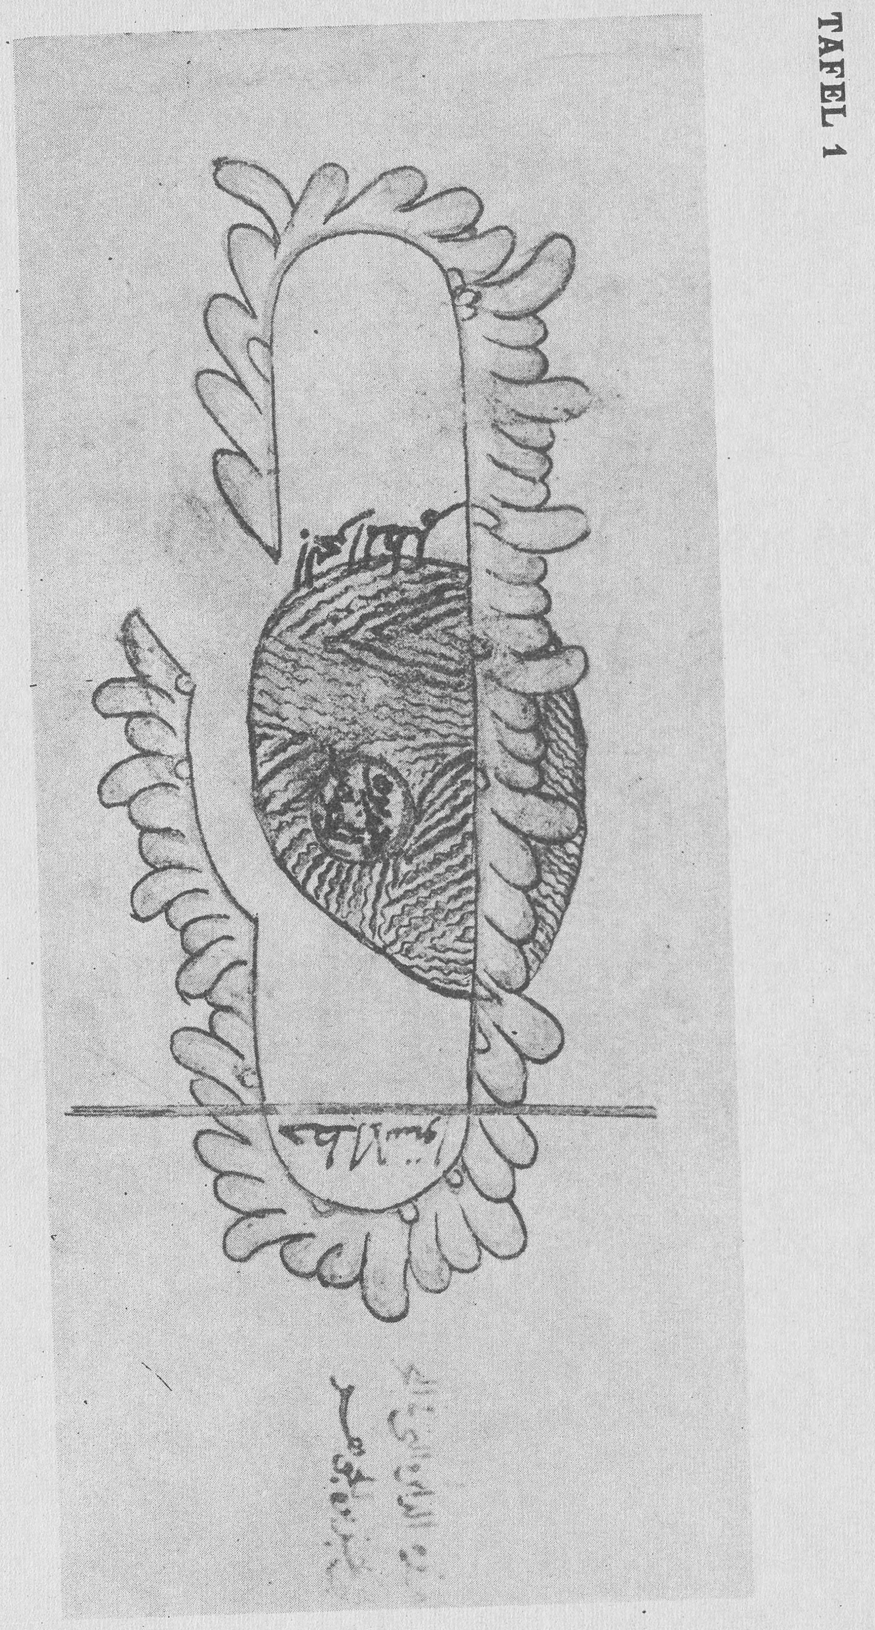
\includegraphics[width=0.8\linewidth,height=0.72\textheight,keepaspectratio]{figures/AK05-F171-FIG1.png}\end{center}\smallskip
\FrameHead{172}{blank}{172}{blank}
\Withheld{blank}
\needspace{0.8\textheight}
\FrameHead{173}{plate}{173}{plate}
\par\smallskip\begin{center}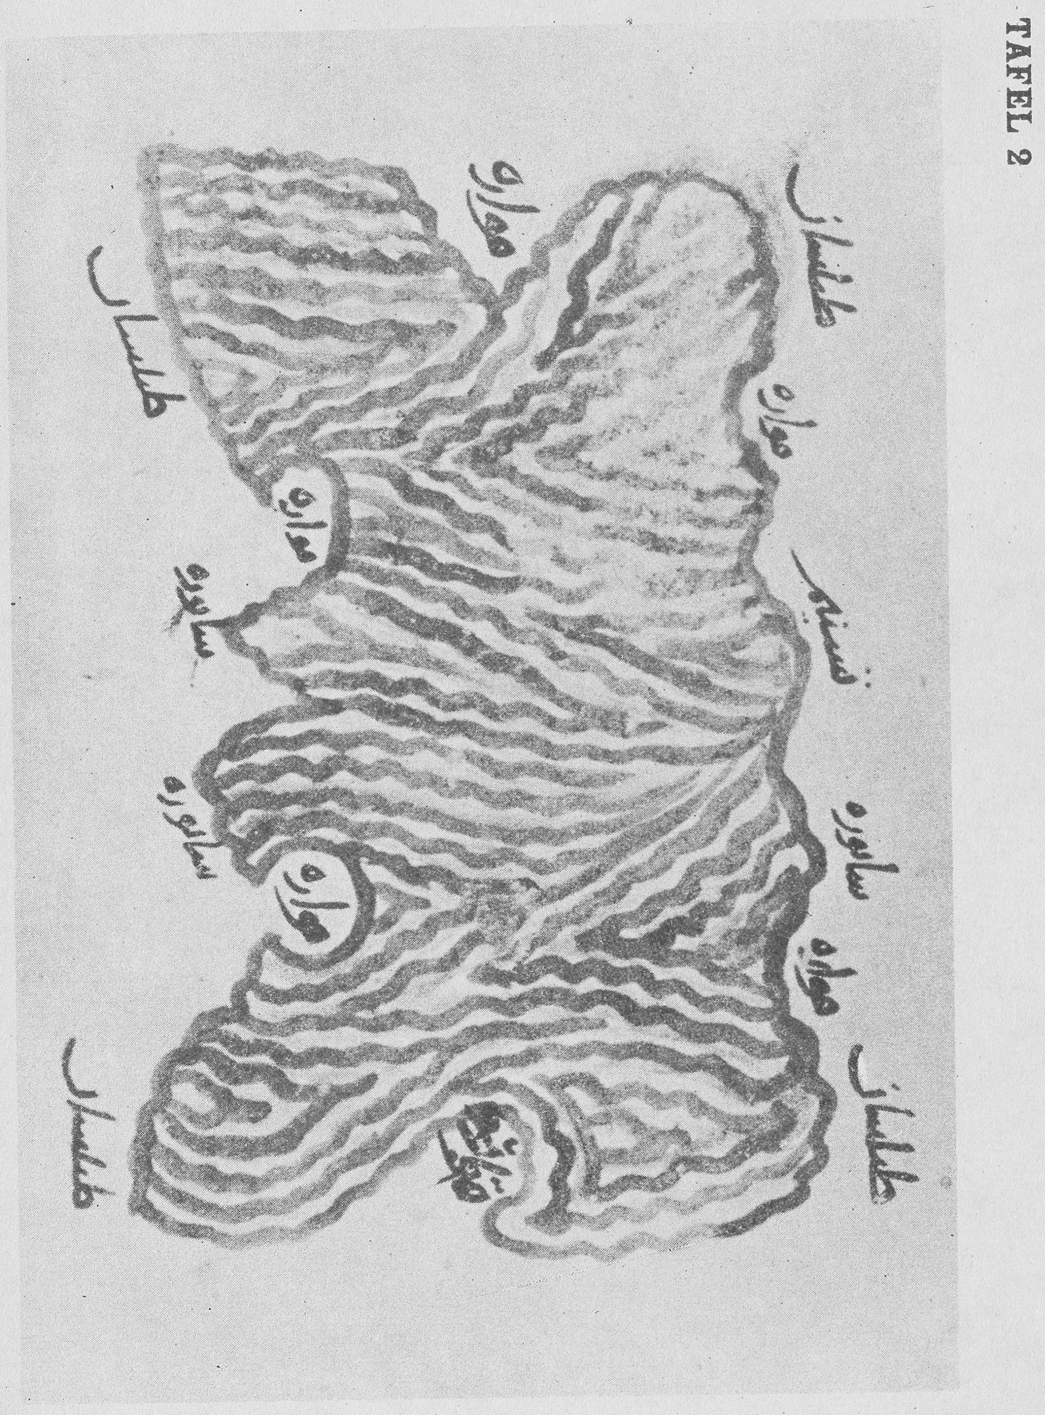
\includegraphics[width=0.8\linewidth,height=0.72\textheight,keepaspectratio]{figures/AK05-F173-FIG1.png}\end{center}\smallskip
\FrameHead{174}{blank}{174}{blank}
\Withheld{blank}
\needspace{0.8\textheight}
\FrameHead{175}{plate}{175}{plate}
\par\smallskip\begin{center}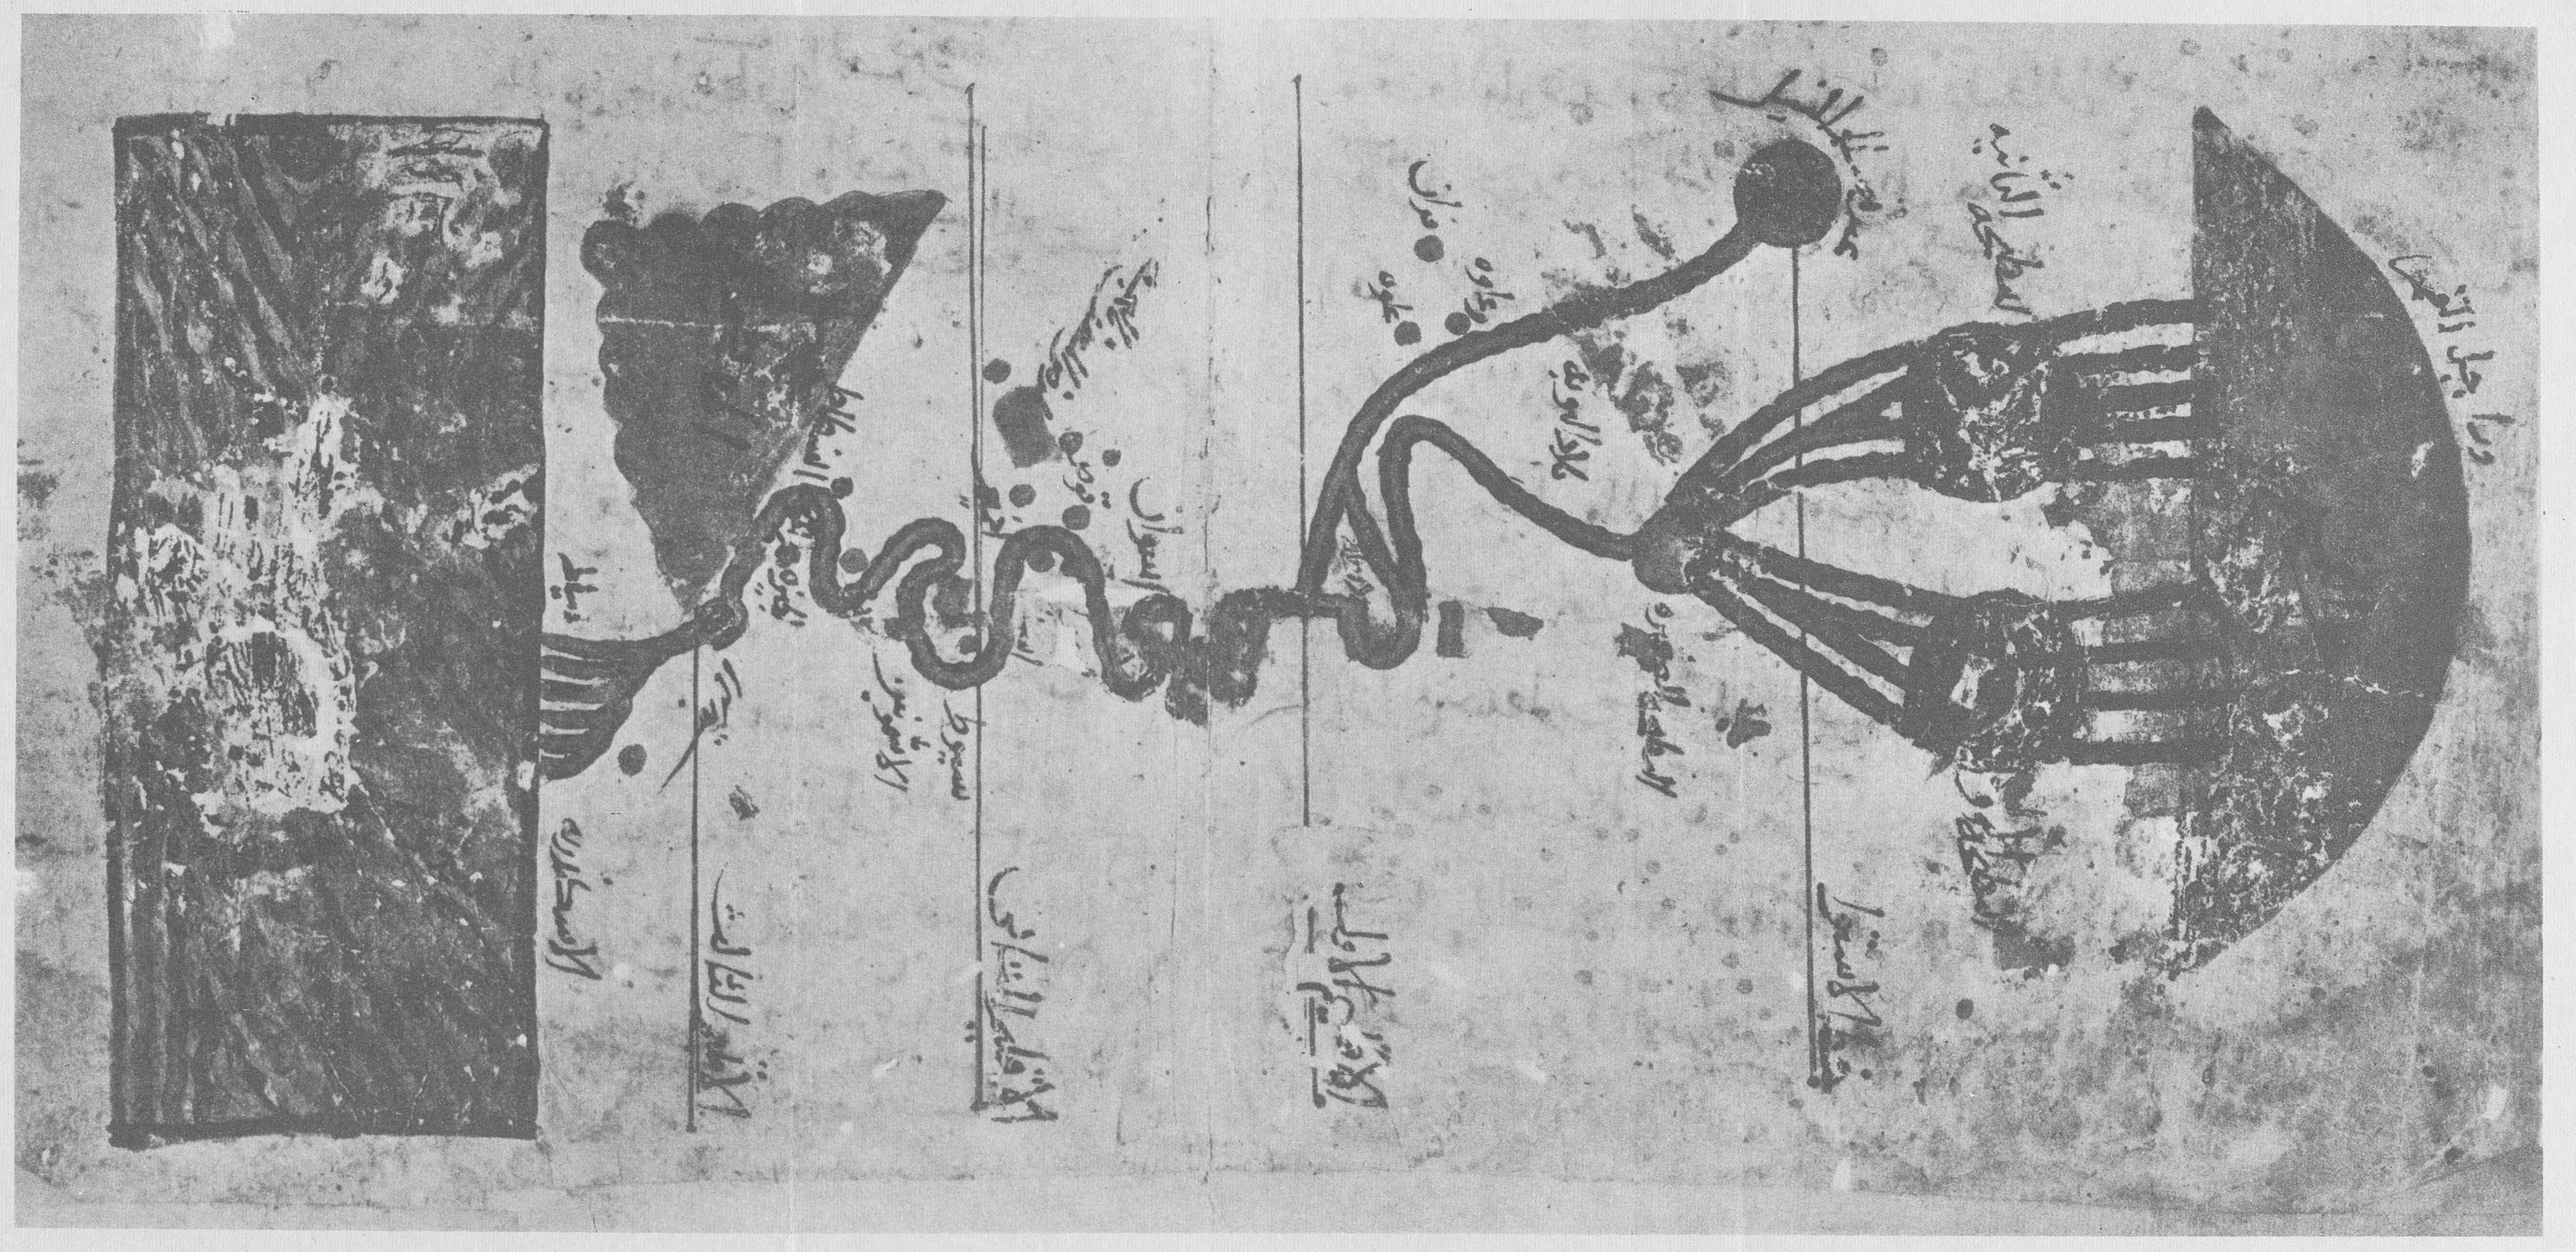
\includegraphics[width=0.8\linewidth,height=0.72\textheight,keepaspectratio]{figures/AK05-F175-FIG1.png}\end{center}\smallskip
\FrameHead{176}{blank}{176}{blank}
\Withheld{blank}
\needspace{0.8\textheight}
\FrameHead{177}{plate}{177}{plate}
\par\smallskip\begin{center}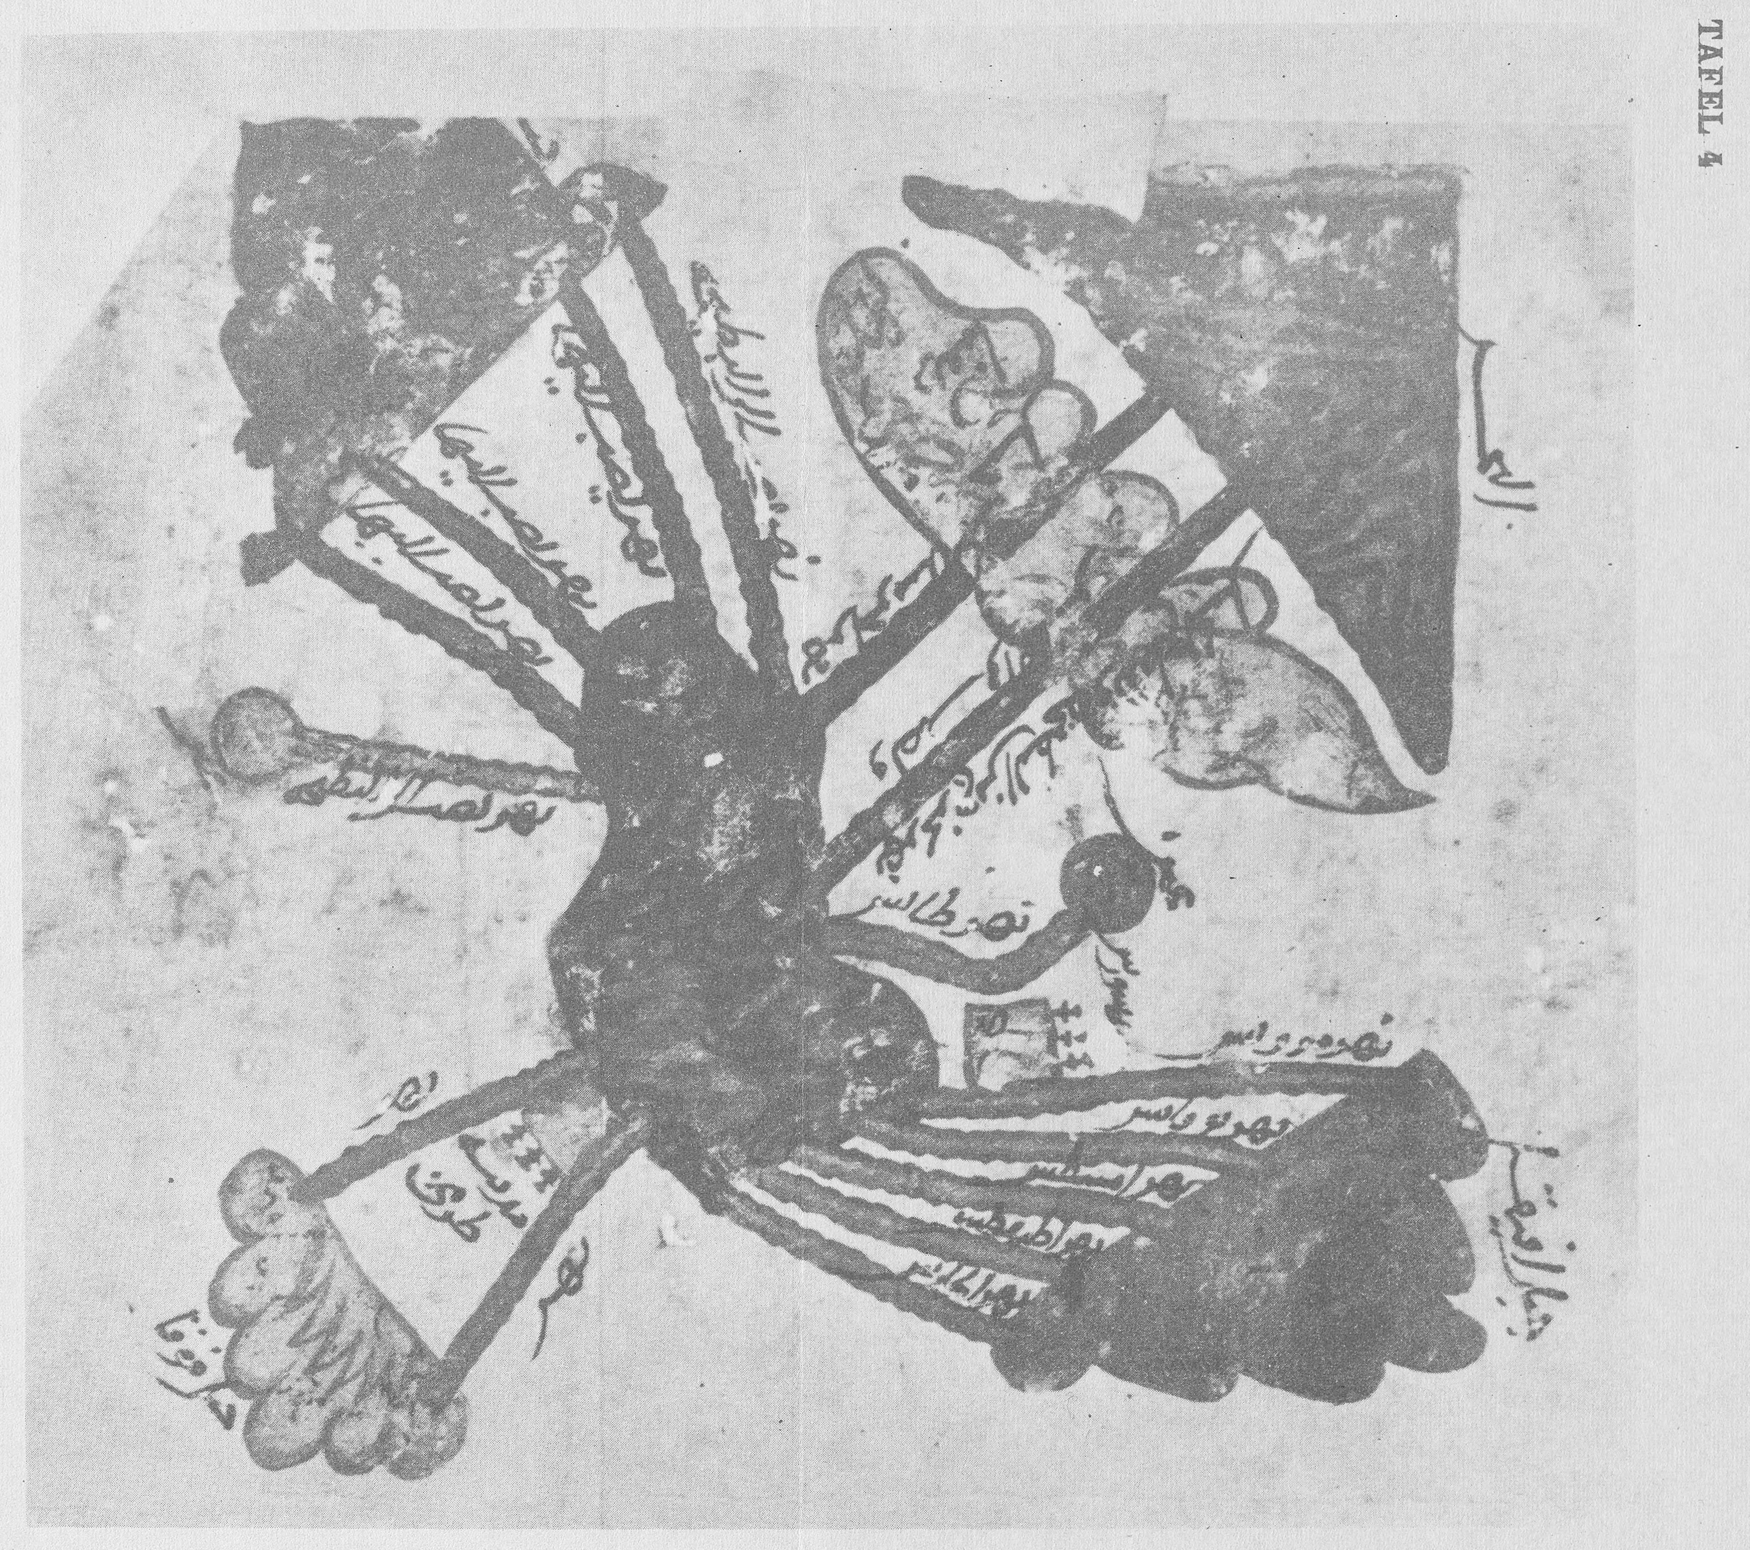
\includegraphics[width=0.8\linewidth,height=0.72\textheight,keepaspectratio]{figures/AK05-F177-FIG1.png}\end{center}\smallskip
\FrameHead{178}{blank}{178}{blank}
\Withheld{blank}
\needspace{0.8\textheight}
\FrameHead{179}{plate}{179}{plate}
\par\smallskip\begin{center}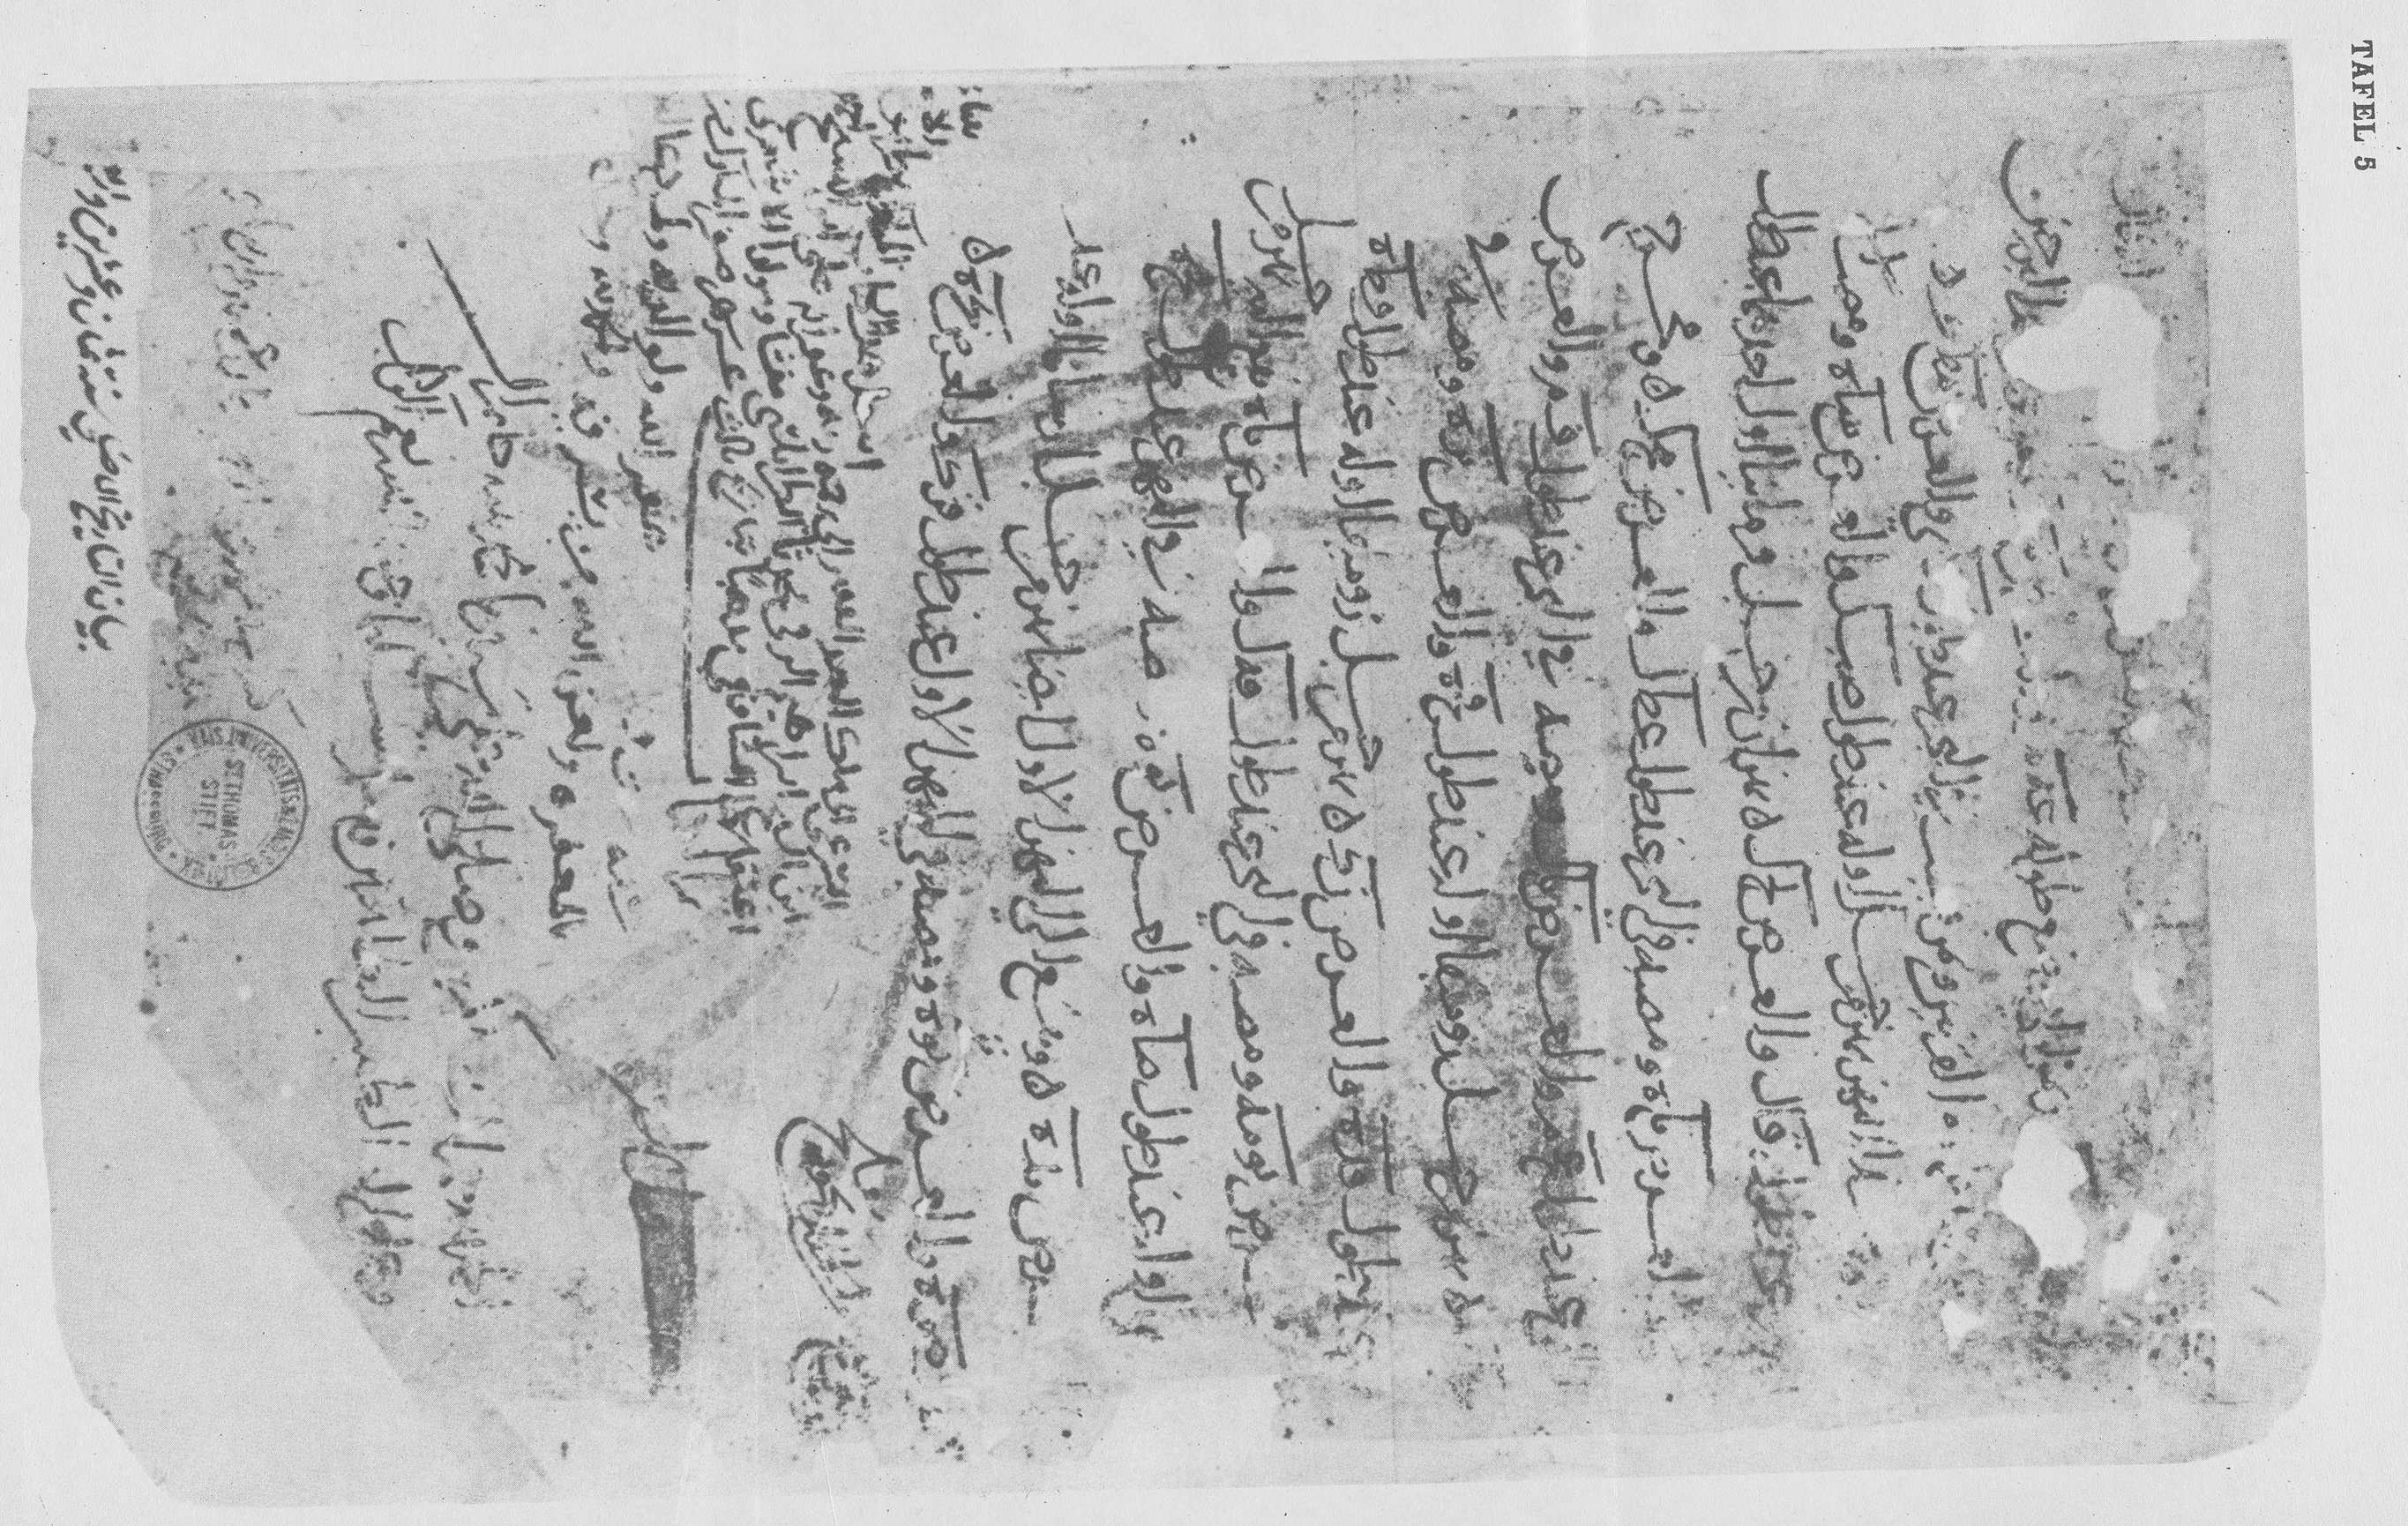
\includegraphics[width=0.8\linewidth,height=0.72\textheight,keepaspectratio]{figures/AK05-F179-FIG1.png}\end{center}\smallskip
\FrameHead{180}{blank}{180}{blank}
\Withheld{blank}
\FrameHead{181}{blank}{181}{blank}
\Withheld{blank}
\FrameHead{182}{p. XXXI}{182}{p. XXXI}
\Withheld{the editor's introduction, p. XXXI, in German: 18 printed lines and the place and date --- not reproduced}
\FrameHead{183}{p. XXX}{183}{p. XXX}
\Withheld{the editor's introduction, p. XXX, in German: 29 printed lines, with words of the text, running numbers and page numbers in Arabic type --- not reproduced}
\FrameHead{184}{p. XXIX}{184}{p. XXIX}
\Withheld{the editor's introduction, p. XXIX, in German: 29 printed lines, with words of the text, running numbers and page numbers in Arabic type --- not reproduced}
\FrameHead{185}{p. XXVIII}{185}{p. XXVIII}
\Withheld{the editor's introduction, p. XXVIII, in German: 24 printed lines, with letters, running numbers and numbers of Suhrāb in Arabic type: the last sections on single letters and a table of groups of letters --- not reproduced}
\FrameHead{186}{p. XXVII}{186}{p. XXVII}
\Withheld{the editor's introduction, p. XXVII, in German: 21 printed lines, with letters and running numbers in Arabic type, in sections headed by the letter they treat --- not reproduced}
\FrameHead{187}{p. XXVI}{187}{p. XXVI}
\Withheld{the editor's introduction, p. XXVI, in German: 24 printed lines, with letters, running numbers and page numbers in Arabic type, in sections headed by the letter they treat --- not reproduced}
\FrameHead{188}{p. XXV}{188}{p. XXV}
\Withheld{the editor's introduction, p. XXV, in German: 24 printed lines, with letters, running numbers and page numbers in Arabic type, in sections headed by the letter they treat --- not reproduced}
\FrameHead{189}{p. XXIV}{189}{p. XXIV}
\Withheld{the editor's introduction, p. XXIV, in German: 24 printed lines, with letters, running numbers and page numbers in Arabic type, in sections headed by the letter they treat --- not reproduced}
\FrameHead{190}{p. XXIII}{190}{p. XXIII}
\Withheld{the editor's introduction, p. XXIII, in German: 29 printed lines, with numerals, running numbers and page numbers in Arabic type and Greek words --- not reproduced}
\FrameHead{191}{p. XXII}{191}{p. XXII}
\Withheld{the editor's introduction, p. XXII, in German: 28 printed lines, with numerals and page numbers in Arabic type --- not reproduced}
\FrameHead{192}{p. XXI}{192}{p. XXI}
\Withheld{the editor's introduction, p. XXI, in German: 29 printed lines, with the forms of the zero sign --- not reproduced}
\FrameHead{193}{p. XX}{193}{p. XX}
\Withheld{the editor's introduction, p. XX, in German: 30 printed lines, with numerals in Arabic type --- not reproduced}
\FrameHead{194}{p. XIX}{194}{p. XIX}
\Withheld{the editor's introduction, p. XIX, in German: 30 printed lines, with numerals and words in Arabic type and a Greek name --- not reproduced}
\FrameHead{195}{p. XVIII}{195}{p. XVIII}
\Withheld{the editor's introduction, p. XVIII, in German: 30 printed lines, with running numbers, page numbers, numerals and words in Arabic type and a Greek name --- not reproduced}
\FrameHead{196}{p. XVII}{196}{p. XVII}
\Withheld{the editor's introduction, p. XVII, in German: 29 printed lines, with numerals in Arabic type --- not reproduced}
\FrameHead{197}{p. XVI}{197}{p. XVI}
\Withheld{the editor's introduction, p. XVI, in German: 30 printed lines, with three page numbers in Arabic-Indic digits --- not reproduced}
\FrameHead{198}{p. XV}{198}{p. XV}
\Withheld{the editor's introduction, p. XV, in German: 30 printed lines, with numerals and two names in Arabic type and Greek names --- not reproduced}
\FrameHead{199}{p. XIV}{199}{p. XIV}
\Withheld{the editor's introduction, p. XIV, in German: 29 printed lines, with running numbers, page numbers and numerals in Arabic type and Greek names --- not reproduced}
\FrameHead{200}{p. XIII}{200}{p. XIII}
\Withheld{the editor's introduction, p. XIII, in German: 30 printed lines, with three running numbers and a Greek name --- not reproduced}
\FrameHead{201}{p. XII}{201}{p. XII}
\Withheld{the editor's introduction, p. XII, in German: 30 printed lines --- not reproduced}
\FrameHead{202}{p. XI}{202}{p. XI}
\Withheld{the editor's introduction, p. XI, in German: 30 printed lines, with running numbers and an Arabic name --- not reproduced}
\FrameHead{203}{p. X}{203}{p. X}
\Withheld{the editor's introduction, p. X, in German: 30 printed lines, with two Arabic names and five running numbers --- not reproduced}
\FrameHead{204}{p. IX}{204}{p. IX}
\Withheld{the editor's introduction, p. IX, in German: 30 printed lines, with four numbers of Suhrāb in Arabic-Indic digits --- not reproduced}
\FrameHead{205}{p. VIII}{205}{p. VIII}
\Withheld{the editor's introduction, p. VIII, in German: 30 printed lines, with running numbers and two names in Arabic type --- not reproduced}
\FrameHead{206}{p. VII}{206}{p. VII}
\Withheld{the editor's introduction, p. VII, in German: 30 printed lines --- not reproduced}
\FrameHead{207}{p. VI}{207}{p. VI}
\Withheld{the editor's introduction, p. VI, in German: 30 printed lines --- not reproduced}
\FrameHead{208}{p. V}{208}{p. V}
\Withheld{the editor's introduction, «EINLEITUNG», p. V, in German: the heading and 24 printed lines --- not reproduced}
\FrameHead{209}{title page}{209}{title page}
\EdLl{1}{AK05-F209-L01}{BUCHDRUCK VON ADOLF HOLZHAUSEN,}{}
\EdLl{2}{AK05-F209-L02}{UNIVERSITÄTSBUCHDRUCKER IN WIEN,}{}
\EdLl{3}{AK05-F209-L03}{VII., KANDLGASSE 19—21}{}
\EdLl{4}{AK05-F209-L04}{LICHTDRUCK VON MAX JAFFÉ,}{}
\EdLl{5}{AK05-F209-L05}{WIEN, XVII., LEOPOLD-ERNST-GASSE 36}{}
\FrameHead{210}{title page}{210}{title page}
\EdLl{1}{AK05-F210-L01}{DAS KITĀB}{}
\EdLl{2}{AK05-F210-L02}{ṢŪRAT AL-ARḌ DES ABŪ ǦAʿFAR}{}
\EdLl{3}{AK05-F210-L03}{MUḤAMMAD IBN MŪSĀ}{}
\EdLl{4}{AK05-F210-L04}{AL-ḪUWĀRIZMĪ}{}
\EdLl{5}{AK05-F210-L05}{Herausgegeben}{}
\EdLl{6}{AK05-F210-L06}{NACH DEM HANDSCHRIFTLICHEN UNIKUM DER}{}
\EdLl{7}{AK05-F210-L07}{BIBLIOTHÈQUE DE L’UNIVERSITÉ ET RÉGIONALE}{}
\EdLl{8}{AK05-F210-L08}{IN STRASSBURG / COD. 4247 /}{}
\EdLl{9}{AK05-F210-L09}{VON}{}
\EdLl{10}{AK05-F210-L10}{HANS v. MŹIK}{}
\EdLl{11}{AK05-F210-L11}{Mit fünf Tafeln in Lichtdruck}{}
\EdLl{12}{AK05-F210-L12}{MCMXXVI}{}
\EdLl{13}{AK05-F210-L13}{Otto Harrassowitz · Leipzig}{}
\FrameHead{211}{blank}{211}{blank}
\Withheld{blank}
\FrameHead{212}{title page}{212}{title page}
\EdLl{1}{AK05-F212-L01}{BIBLIOTHEK}{}
\EdLl{2}{AK05-F212-L02}{ARABISCHER HISTORIKER}{}
\EdLl{3}{AK05-F212-L03}{UND GEOGRAPHEN}{}
\EdLl{4}{AK05-F212-L04}{HERAUSGEGEBEN VON}{}
\EdLl{5}{AK05-F212-L05}{HANS v. MŽIK}{}
\EdLl{6}{AK05-F212-L06}{Dritter Band:}{}
\EdLl{7}{AK05-F212-L07}{DAS KITĀB ṢŪRAT AL-ARḌ}{}
\EdLl{8}{AK05-F212-L08}{DES ABŪ ǦAʿFAR MUḤAMMAD}{}
\EdLl{9}{AK05-F212-L09}{IBN MŪSĀ AL-ḪUWĀRIZMĪ}{}
\EdLl{10}{AK05-F212-L10}{Arabischer Text}{}
\EdLl{11}{AK05-F212-L11}{MCMXXVI}{}
\EdLl{12}{AK05-F212-L12}{Otto Harrassowitz · Leipzig}{}
\FrameHead{213}{blank}{213}{blank}
\Withheld{blank}
\FrameHead{214}{title page}{214}{title page}
\EdLl{1}{AK05-F214-L01}{DAS KITĀB}{}
\EdLl{2}{AK05-F214-L02}{ṢŪRAT AL-ARḌ DES ABŪ ǦAʿFAR}{}
\EdLl{3}{AK05-F214-L03}{MUḤAMMAD IBN MŪSĀ}{}
\EdLl{4}{AK05-F214-L04}{AL-ḪUWĀRIZMĪ}{}
\EdLl{5}{AK05-F214-L05}{Herausgegeben}{}
\EdLl{6}{AK05-F214-L06}{NACH DEM HANDSCHRIFTLICHEN UNIKUM DER}{}
\EdLl{7}{AK05-F214-L07}{BIBLIOTHÈQUE DE L’UNIVERSITÉ ET RÉGIONALE}{}
\EdLl{8}{AK05-F214-L08}{IN STRASSBURG / COD. 4247 /}{}
\EdLl{9}{AK05-F214-L09}{VON}{}
\EdLl{10}{AK05-F214-L10}{HANS v. MŹIK}{}
\EdLl{11}{AK05-F214-L11}{Mit fünf Tafeln in Lichtdruck}{}
\EdLl{12}{AK05-F214-L12}{MCMXXVI}{}
\EdLl{13}{AK05-F214-L13}{Otto Harrassowitz · Leipzig}{}
\FrameHead{215}{blank}{215}{blank}
\Withheld{blank}
\FrameHead{216}{blank}{216}{blank}
\Withheld{blank}
\FrameHead{217}{library matter}{217}{library matter}
\Withheld{library matter only: The barcode label «COLUMBIA UNIVERSITY LIBRARIES», number «0050628623», at the top of the endpaper, with pencil strokes scribbled across it; not part of the edition.}
\FrameHead{218}{binding}{218}{binding}
\Withheld{the library's binding: The back board of the library's binding, in blue cloth, worn along the spine; at the top a label «COLUMBIA LIBRARIES OFFSITE» with a barcode, the number «CU70324743», the call number «G93 .K48» and the short title «Kitab surat al-ard m…»; not part of the edition.}
\clearpage\pdfbookmark[1]{critical notes}{critical}{\large\bfseries Critical notes}\par\medskip\noindent These notes are not part of the transcription. They record errors of the print and propose corrections; the transcription keeps the print.\par\medskip
\noindent\textbf{AK05-CN017}\enspace\hyperlink{AK05-F023-L13}{AK05-F023-L13}\enspace(corrected in the corrigenda)\par\noindent printed: \RL{\ArBody ٮرقه}\enspace proposed: \RL{\ArBody برقة}\par\noindent the editor's list of additions and corrections on p. 163 (frame 169) reads \RL{\ArBody برقة} for \RL{\ArBody ٮرقه} in this line, p. 17, line 13\par\noindent confidence: high\par\noindent impact: the name of entry 225 reads \RL{\ArBody برقة}, Barqa\par\medskip
\noindent\textbf{AK05-CN018}\enspace\hyperlink{AK05-F024-L18}{AK05-F024-L18}\enspace(corrected in the corrigenda)\par\noindent printed: \RL{\ArBody قٮرس}\enspace proposed: \RL{\ArBody قبرس}\par\noindent the editor's list of additions and corrections on p. 163 (frame 169) reads \RL{\ArBody قبرس} for \RL{\ArBody قٮرس} in this line, p. 18, line 18; his note e gives \RL{\ArBody قٮرس} as the reading of the manuscript, and the next page prints the island \RL{\ArBody قبرس} with the dot of the \RL{\ArBody ب} (frame 025, L06, L09)\par\noindent confidence: high\par\noindent impact: the island of entry 248 reads \RL{\ArBody قبرس}, Cyprus\par\medskip
\noindent\textbf{AK05-CN001}\enspace\hyperlink{AK05-F026-L13}{AK05-F026-L13}\enspace(wrong number)\par\noindent printed: (\RL{\ArBody ٧٨٠})\enspace proposed: (\RL{\ArBody ٢٨٠})\par\noindent the running numbers of the page go from (\RL{\ArBody ٢٧٩}) in L12 to (\RL{\ArBody ٢٨١}) in L14, and the first digit is a \RL{\ArBody ٧}, printed like the \RL{\ArBody ٧} of (\RL{\ArBody ٢٧٩}); the editor's notes do not comment on it\par\noindent confidence: high\par\noindent impact: none on the table: the running number only counts the entries\par\medskip
\noindent\textbf{AK05-CN019}\enspace\hyperlink{AK05-F026-L08}{AK05-F026-L08}\enspace(corrected in the corrigenda)\par\noindent printed: \RL{\ArBody المصيصة}\enspace proposed: \RL{\ArBody المصّيصة}\par\noindent the editor's list of additions and corrections on p. 163 (frame 169) reads \RL{\ArBody المصّيصة}, with a shadda over the \RL{\ArBody ص}, for \RL{\ArBody المصيصة} in this line, p. 20, line 8\par\noindent confidence: high\par\noindent impact: a vowel sign only: the name of entry 275 reads al-Maṣṣīṣa\par\medskip
\noindent\textbf{AK05-CN002}\enspace\hyperlink{AK05-F030-L14}{AK05-F030-L14}\enspace(wrong or turned sort)\par\noindent printed: ]\RL{\ArBody ٢٩٤}]\enspace proposed: [\RL{\ArBody ٢٩٤}]\par\noindent the bracket that opens the number of Suhrāb, at the right in the line, has the form of the closing bracket (the printed form is given in the order of reading; from left to right the page shows [\RL{\ArBody ٢٩٤}[, two brackets of one form), where the brackets of the other entries face each other\par\noindent confidence: high\par\noindent impact: none: the number reads 294 either way\par\medskip
\noindent\textbf{AK05-CN003}\enspace\hyperlink{AK05-F032-L17}{AK05-F032-L17}\enspace(missing letter)\par\noindent printed: (\RL{\ArBody ٣ ٤})\enspace proposed: (\RL{\ArBody ٣٨٤})\par\noindent the running number of entry 384 is printed with a blank where its middle digit stands, between (\RL{\ArBody ٣٨٣}) in L16 and (\RL{\ArBody ٣٨٥}) on the next page; a speck of 5 px in the blank is all that shows of the digit, which has not printed\par\noindent confidence: high\par\noindent impact: none on the table: the running number only counts the entries\par\medskip
\noindent\textbf{AK05-CN020}\enspace\hyperlink{AK05-F035-L07}{AK05-F035-L07}\enspace(corrected in the corrigenda)\par\noindent printed: \RL{\ArBody لج}\enspace proposed: \RL{\ArBody لح}\par\noindent the editor's list of additions and corrections on p. 163 (frame 169) reads \RL{\ArBody لح} for \RL{\ArBody لج} in this line, p. 29, line 7, where \RL{\ArBody لج} is the degrees of the latitude of al-Andalus\par\noindent confidence: high\par\noindent impact: the latitude of al-Andalus, entry 419, reads 38° 0′ instead of 33° 0′\par\medskip
\noindent\textbf{AK05-CN004}\enspace\hyperlink{AK05-F053-L11}{AK05-F053-L11}\enspace(misplaced dot)\par\noindent printed: \RL{\ArBody جبوب}\enspace proposed: \RL{\ArBody جنوب}\par\noindent the dot of the second letter of the direction stands below the tooth, beside the dot of the \RL{\ArBody ج}, and none stands above it, where the direction \RL{\ArBody جنوب} of L08, L10 and L15 has the dot of the \RL{\ArBody ن} above the tooth; \RL{\ArBody جبوب} is not a word, and the directions of the table are \RL{\ArBody جنوب}, \RL{\ArBody شمال}, \RL{\ArBody مشرقىّ} and \RL{\ArBody مغربىّ}\par\noindent confidence: high\par\noindent impact: none on the coordinates; the direction of the head is south\par\medskip
\noindent\textbf{AK05-CN005}\enspace\hyperlink{AK05-F071-L02}{AK05-F071-L02}\enspace(stray dot)\par\noindent printed: \RL{\ArBody ضه}\enspace proposed: \RL{\ArBody صه}\par\noindent the degrees of the first longitude are printed with a \RL{\ArBody ض}, 800, which gives 805, beyond the longitudes of the table, which all lie below 180; the dot above the bowl is 6 by 6 px, smaller than the dots of the font, 9 by 9 px, and without it the letter is \RL{\ArBody ص}, 90, which gives 95, beside the first longitudes 89 and 97 of L01 and L04; the editor's note b records that the manuscript has \RL{\ArBody مه} here by mistake\par\noindent confidence: high\par\noindent impact: the longitude of the first boundary of entry 931/932: 95° 40′ for 805° 40′\par\medskip
\noindent\textbf{AK05-CN006}\enspace\hyperlink{AK05-F078-L01}{AK05-F078-L01}\enspace(wrong sort)\par\noindent printed: (fol, 18ᵃ)\enspace proposed: (fol. 18ᵃ)\par\noindent the folio of the manuscript is printed with a comma after «fol», where every other folio marked in the edition read so far, from «(fol. 2ᵇ)» (frame 009) to «(fol. 17ᵇ)» (frame 076), has a full stop\par\noindent confidence: high\par\noindent impact: none: the folio reads 18ᵃ either way\par\medskip
\noindent\textbf{AK05-CN021}\enspace\hyperlink{AK05-F085-L12}{AK05-F085-L12}\enspace(corrected in the corrigenda)\par\noindent printed: \RL{\ArBody بٮ ن}\enspace proposed: \RL{\ArBody يٮ ن}\par\noindent the editor's list of additions and corrections on p. 163 (frame 169) reads \RL{\ArBody يٮ ن} for \RL{\ArBody بٮ ن} in this line, p. 79, line 12, both followed by the note mark n; the latitude, 12° 50′ read with the \RL{\ArBody ي}, lies between the latitudes of 14° to 18° 50′ and of 10° 20′ of the points before and after it (L11, L13, L15)\par\noindent confidence: high\par\noindent impact: the latitude of point 1221 reads 12° 50′\par\medskip
\noindent\textbf{AK05-CN007}\enspace\hyperlink{AK05-F097-L11}{AK05-F097-L11}\enspace(stray dot)\par\noindent printed: \RL{\ArBody والغرض}\enspace proposed: \RL{\ArBody والعرض}\par\noindent the word before the latitude of island 1404 has a dot over the \RL{\ArBody ع}, which makes it \RL{\ArBody غ}; «\RL{\ArBody والغرض}», and the purpose, gives no sense before the numerals, where every other island of the page and of the section has «\RL{\ArBody والعرض}», and the latitude; the dot is of the size of the dots of the font, 10 by 7 px, and stands where the dot of a \RL{\ArBody غ} would stand\par\noindent confidence: high\par\noindent impact: none: the numerals give the latitude of island 1404 either way\par\medskip
\noindent\textbf{AK05-CN008}\enspace\hyperlink{AK05-F110-L10}{AK05-F110-L10}\enspace(damaged or wrong sort)\par\noindent printed: \RL{\ArBody عنا}\enspace proposed: \RL{\ArBody عند}\par\noindent the word between «\RL{\ArBody وسطها}» and «\RL{\ArBody طول}» of entry 1591 ends in a vertical stroke without the foot of the \RL{\ArBody د}, so that it reads «\RL{\ArBody عنا}», which gives no sense there; every other entry of the section has «\RL{\ArBody وسطها عند طول}», and the \RL{\ArBody د} of «\RL{\ArBody عند}» in L02 has its foot\par\noindent confidence: high\par\noindent impact: none: the coordinates read the same\par\medskip
\noindent\textbf{AK05-CN009}\enspace\hyperlink{AK05-F115-L08}{AK05-F115-L08}\enspace(wrong sort)\par\noindent printed: [\RL{\ArBody ١٥٥٠})\enspace proposed: [\RL{\ArBody ١٥٥٠}]\par\noindent the number of Suhrāb of point 1654 is closed by a round parenthesis, of the height and form of those of the running numbers, where every other number of Suhrāb of the page and of the edition read so far is closed by a square bracket, as [\RL{\ArBody ١٥٤٩}] at the beginning of the same line\par\noindent confidence: high\par\noindent impact: none: the number reads 1550 either way\par\medskip
\noindent\textbf{AK05-CN010}\enspace\hyperlink{AK05-F124-L04}{AK05-F124-L04}\enspace(missing letter)\par\noindent printed: [\RL{\ArBody ١٧٨} ]\enspace proposed: [\RL{\ArBody ١٧٨٤}]\par\noindent the number of Suhrāb of point 1779 is printed with a blank where its last digit stands, before the opening bracket at the right, which is printed faint and broken, between [\RL{\ArBody ١٧٨٣}] in L03 and [\RL{\ArBody ١٧٨٥}] in L05\par\noindent confidence: high\par\noindent impact: none: the number of Suhrāb only counts the points\par\medskip
\noindent\textbf{AK05-CN011}\enspace\hyperlink{AK05-F125-L01}{AK05-F125-L01}\enspace(missing sort)\par\noindent printed: \ensuremath{\langle}\RL{\ArBody الإق}ᵃ\RL{\ArBody ليم}\enspace proposed: \ensuremath{\langle}\RL{\ArBody الإق}\ensuremath{\rangle}ᵃ\RL{\ArBody ليم}\par\noindent the angle bracket that opens before «\RL{\ArBody الإق}» in the heading is not closed: the note mark a follows the \RL{\ArBody ق}, which is printed in its final form and not joined to the \RL{\ArBody ل} of «\RL{\ArBody ليم}», where the other supplied passages of the page, «\ensuremath{\langle}\RL{\ArBody الأنهار}\ensuremath{\rangle}» in the same line and those of L02, L04 and L05, close with a bracket before their note mark\par\noindent confidence: high\par\noindent impact: the extent of the supplied letters; the words read the same\par\medskip
\noindent\textbf{AK05-CN012}\enspace\hyperlink{AK05-F130-L06}{AK05-F130-L06}\enspace(stray dot)\par\noindent printed: \RL{\ArBody غند}\enspace proposed: \RL{\ArBody عند}\par\noindent the first word of the line, before «\RL{\ArBody طول}», has a mark of the size of the dots of the font, 10 by 13 px, over the initial \RL{\ArBody ع}, which makes it \RL{\ArBody غ}; «\RL{\ArBody غند}» is not a word, where every other «\RL{\ArBody عند}» of the page, eighteen of them, has none\par\noindent confidence: high\par\noindent impact: none: the coordinates read the same\par\medskip
\noindent\textbf{AK05-CN013}\enspace\hyperlink{AK05-F143-L04}{AK05-F143-L04}\enspace(missing letter)\par\noindent printed: (\RL{\ArBody ٢ ٧٨})\enspace proposed: (\RL{\ArBody ٢٠٧٨})\par\noindent the running number of the point after (\RL{\ArBody ٢٠٧٧}) is printed with a blank where its zero stands, between (\RL{\ArBody ٢٠٧٧}) in L03 and (\RL{\ArBody ٢٠٧٩}) in L05\par\noindent confidence: high\par\noindent impact: none: the running numbers only count the points\par\medskip
\noindent\textbf{AK05-CN014}\enspace\hyperlink{AK05-F149-L05}{AK05-F149-L05}\enspace(missing note mark)\par\noindent printed: \RL{\ArBody مو يه}\enspace proposed: \RL{\ArBody مو يه}\{n:i\}\par\noindent the footnotes print a note i, a variant reading \RL{\ArBody مز يه} with a line over it, between note h, whose mark follows the longitude of L05, and note k, whose mark stands in L09, while the text has no mark i; the latitude of L05, «\RL{\ArBody مو يه}», differs from the variant in one letter, \RL{\ArBody و} for \RL{\ArBody ز}\par\noindent confidence: medium\par\noindent impact: the place of the variant reading; the longitude «\RL{\ArBody م يه}» of L07 is the other possible place\par\medskip
\noindent\textbf{AK05-CN015}\enspace\hyperlink{AK05-F159-L12}{AK05-F159-L12}\enspace(wrong reference)\par\noindent printed: p. 150, note g\enspace proposed: p. 150, note h\par\noindent the editor's note e, at the folio «(fol. 46ᵃ)», refers for the order of the leaves of the manuscript to note g of p. 150; on that page the note on the order of the leaves, at the folio «(fol. 35ᵃ)», is note h (frame 156, L14), and note g is the note on the supplied word «\ensuremath{\langle}\RL{\ArBody عين}\ensuremath{\rangle}» (frame 156, L13)\par\noindent confidence: high\par\noindent impact: none on the text: the reference of the editor's note\par\medskip
\noindent\textbf{AK05-CN016}\enspace\hyperlink{AK05-F166-L06}{AK05-F166-L06}\enspace(stray sort)\par\noindent printed: \RL{\ArBody الأرض ا المعمورة}\enspace proposed: \RL{\ArBody الأرض المعمورة}\par\noindent the head of the seas has an isolated alif between «\RL{\ArBody الأرض}» and «\RL{\ArBody المعمورة}», set off by a word space on each side, of the size of the alifs of these two words, 11 by 52 px; the heads of the cities and of the mountains on p. 159 (frame 165, L02 and L13) read «\RL{\ArBody على كرة الأرض المعمورة}» without it, and so does the head of the seas in the text on p. 66 (frame 072, L01), «\RL{\ArBody البحار الّتى على كرة الأرض المعمورة وجزائرها}»\par\noindent confidence: high\par\noindent impact: none: the head reads the same without it\par\medskip
\noindent\textbf{AK05-CN022}\enspace\hyperlink{AK05-F210-L10}{AK05-F210-L10}\enspace(wrong accent)\par\noindent printed: MŹIK\enspace proposed: MŽIK\par\noindent the editor's name is printed with an acute accent over the Z, where the series title page of the same volume prints it with a haček, «HANS v. MŽIK» (frame 212, L04), the spelling of the name Mžik; the reprint's copy of this page has the same acute (frame 214, L10)\par\noindent confidence: medium\par\noindent impact: the name of the editor, Hans von Mžik\par\medskip
\end{document}
